\documentclass[twoside]{book}

% Packages required by doxygen
\usepackage{fixltx2e}
\usepackage{calc}
\usepackage{doxygen}
\usepackage[export]{adjustbox} % also loads graphicx
\usepackage{graphicx}
\usepackage[utf8]{inputenc}
\usepackage{makeidx}
\usepackage{multicol}
\usepackage{multirow}
\PassOptionsToPackage{warn}{textcomp}
\usepackage{textcomp}
\usepackage[nointegrals]{wasysym}
\usepackage[table]{xcolor}

% Font selection
\usepackage[T1]{fontenc}
\usepackage[scaled=.90]{helvet}
\usepackage{courier}
\usepackage{amssymb}
\usepackage{sectsty}
\renewcommand{\familydefault}{\sfdefault}
\allsectionsfont{%
  \fontseries{bc}\selectfont%
  \color{darkgray}%
}
\renewcommand{\DoxyLabelFont}{%
  \fontseries{bc}\selectfont%
  \color{darkgray}%
}
\newcommand{\+}{\discretionary{\mbox{\scriptsize$\hookleftarrow$}}{}{}}

% Page & text layout
\usepackage{geometry}
\geometry{%
  a4paper,%
  top=2.5cm,%
  bottom=2.5cm,%
  left=2.5cm,%
  right=2.5cm%
}
\tolerance=750
\hfuzz=15pt
\hbadness=750
\setlength{\emergencystretch}{15pt}
\setlength{\parindent}{0cm}
\setlength{\parskip}{3ex plus 2ex minus 2ex}
\makeatletter
\renewcommand{\paragraph}{%
  \@startsection{paragraph}{4}{0ex}{-1.0ex}{1.0ex}{%
    \normalfont\normalsize\bfseries\SS@parafont%
  }%
}
\renewcommand{\subparagraph}{%
  \@startsection{subparagraph}{5}{0ex}{-1.0ex}{1.0ex}{%
    \normalfont\normalsize\bfseries\SS@subparafont%
  }%
}
\makeatother

% Headers & footers
\usepackage{fancyhdr}
\pagestyle{fancyplain}
\fancyhead[LE]{\fancyplain{}{\bfseries\thepage}}
\fancyhead[CE]{\fancyplain{}{}}
\fancyhead[RE]{\fancyplain{}{\bfseries\leftmark}}
\fancyhead[LO]{\fancyplain{}{\bfseries\rightmark}}
\fancyhead[CO]{\fancyplain{}{}}
\fancyhead[RO]{\fancyplain{}{\bfseries\thepage}}
\fancyfoot[LE]{\fancyplain{}{}}
\fancyfoot[CE]{\fancyplain{}{}}
\fancyfoot[RE]{\fancyplain{}{\bfseries\scriptsize Generated by Doxygen }}
\fancyfoot[LO]{\fancyplain{}{\bfseries\scriptsize Generated by Doxygen }}
\fancyfoot[CO]{\fancyplain{}{}}
\fancyfoot[RO]{\fancyplain{}{}}
\renewcommand{\footrulewidth}{0.4pt}
\renewcommand{\chaptermark}[1]{%
  \markboth{#1}{}%
}
\renewcommand{\sectionmark}[1]{%
  \markright{\thesection\ #1}%
}

% Indices & bibliography
\usepackage{natbib}
\usepackage[titles]{tocloft}
\setcounter{tocdepth}{3}
\setcounter{secnumdepth}{5}
\makeindex

% Hyperlinks (required, but should be loaded last)
\usepackage{ifpdf}
\ifpdf
  \usepackage[pdftex,pagebackref=true]{hyperref}
\else
  \usepackage[ps2pdf,pagebackref=true]{hyperref}
\fi
\hypersetup{%
  colorlinks=true,%
  linkcolor=blue,%
  citecolor=blue,%
  unicode%
}

% Custom commands
\newcommand{\clearemptydoublepage}{%
  \newpage{\pagestyle{empty}\cleardoublepage}%
}

\usepackage{caption}
\captionsetup{labelsep=space,justification=centering,font={bf},singlelinecheck=off,skip=4pt,position=top}

%===== C O N T E N T S =====

\begin{document}

% Titlepage & ToC
\hypersetup{pageanchor=false,
             bookmarksnumbered=true,
             pdfencoding=unicode
            }
\pagenumbering{alph}
\begin{titlepage}
\vspace*{7cm}
\begin{center}%
{\Large Schmou\textquotesingle{}T\+SE \\[1ex]\large 0.\+1 }\\
\vspace*{1cm}
{\large Generated by Doxygen 1.8.14}\\
\end{center}
\end{titlepage}
\clearemptydoublepage
\pagenumbering{roman}
\tableofcontents
\clearemptydoublepage
\pagenumbering{arabic}
\hypersetup{pageanchor=true}

%--- Begin generated contents ---
\chapter{Namespace Index}
\section{Namespace List}
Here is a list of all namespaces with brief descriptions\+:\begin{DoxyCompactList}
\item\contentsline{section}{\mbox{\hyperlink{namespacestd}{std}} }{\pageref{namespacestd}}{}
\item\contentsline{section}{\mbox{\hyperlink{namespacestd_1_1experimental}{std\+::experimental}} }{\pageref{namespacestd_1_1experimental}}{}
\item\contentsline{section}{\mbox{\hyperlink{namespacestd_1_1experimental_1_1detail__}{std\+::experimental\+::detail\+\_\+}} }{\pageref{namespacestd_1_1experimental_1_1detail__}}{}
\end{DoxyCompactList}

\chapter{Hierarchical Index}
\section{Class Hierarchy}
This inheritance list is sorted roughly, but not completely, alphabetically\+:\begin{DoxyCompactList}
\item \contentsline{section}{Bouton\+Capacite}{\pageref{class_bouton_capacite}}{}
\item \contentsline{section}{Capacite}{\pageref{class_capacite}}{}
\begin{DoxyCompactList}
\item \contentsline{section}{Cap\+Aim\+Bot}{\pageref{class_cap_aim_bot}}{}
\item \contentsline{section}{Cap\+Bismillah}{\pageref{class_cap_bismillah}}{}
\item \contentsline{section}{Cap\+Boing}{\pageref{class_cap_boing}}{}
\item \contentsline{section}{Cap\+Bouclier\+Rond}{\pageref{class_cap_bouclier_rond}}{}
\item \contentsline{section}{Cap\+Dash}{\pageref{class_cap_dash}}{}
\item \contentsline{section}{Cap\+Missile}{\pageref{class_cap_missile}}{}
\item \contentsline{section}{Cap\+Piou}{\pageref{class_cap_piou}}{}
\end{DoxyCompactList}
\item \contentsline{section}{case\+Insensitive\+Compare}{\pageref{structcase_insensitive_compare}}{}
\item \contentsline{section}{Chargeur}{\pageref{class_chargeur}}{}
\item \contentsline{section}{std\+:\+:experimental\+:\+:constexpr\+\_\+optional\+\_\+base$<$ T $>$}{\pageref{structstd_1_1experimental_1_1constexpr__optional__base}}{}
\item \contentsline{section}{std\+:\+:experimental\+:\+:constexpr\+\_\+storage\+\_\+t$<$ T $>$}{\pageref{unionstd_1_1experimental_1_1constexpr__storage__t}}{}
\item \contentsline{section}{Ecran}{\pageref{class_ecran}}{}
\begin{DoxyCompactList}
\item \contentsline{section}{Accueil}{\pageref{class_accueil}}{}
\item \contentsline{section}{Menu\+Principal}{\pageref{class_menu_principal}}{}
\item \contentsline{section}{Partie}{\pageref{class_partie}}{}
\begin{DoxyCompactList}
\item \contentsline{section}{Pattern}{\pageref{class_pattern}}{}
\end{DoxyCompactList}
\end{DoxyCompactList}
\item \contentsline{section}{Element\+Vague}{\pageref{struct_element_vague}}{}
\item \contentsline{section}{Entite}{\pageref{class_entite}}{}
\begin{DoxyCompactList}
\item \contentsline{section}{Projectile}{\pageref{class_projectile}}{}
\begin{DoxyCompactList}
\item \contentsline{section}{Proj\+Bismillah}{\pageref{class_proj_bismillah}}{}
\item \contentsline{section}{Proj\+Boing}{\pageref{class_proj_boing}}{}
\item \contentsline{section}{Proj\+Bouclier\+Rond}{\pageref{class_proj_bouclier_rond}}{}
\item \contentsline{section}{Proj\+Missile}{\pageref{class_proj_missile}}{}
\item \contentsline{section}{Proj\+Piou}{\pageref{class_proj_piou}}{}
\end{DoxyCompactList}
\item \contentsline{section}{Vaisseau}{\pageref{class_vaisseau}}{}
\begin{DoxyCompactList}
\item \contentsline{section}{Vaiss\+Bouclier}{\pageref{class_vaiss_bouclier}}{}
\item \contentsline{section}{Vaisseau\+Attaquant}{\pageref{class_vaisseau_attaquant}}{}
\item \contentsline{section}{Vaisseau\+Defenseur}{\pageref{class_vaisseau_defenseur}}{}
\item \contentsline{section}{Vaisseau\+Eclaireur}{\pageref{class_vaisseau_eclaireur}}{}
\item \contentsline{section}{Vaisseau\+Test}{\pageref{class_vaisseau_test}}{}
\end{DoxyCompactList}
\end{DoxyCompactList}
\item \contentsline{section}{std\+:\+:experimental\+:\+:is\+\_\+nothrow\+\_\+move\+\_\+assignable$<$ T $>$\+:\+:has\+\_\+nothrow\+\_\+move\+\_\+assign$<$ X, has\+\_\+any\+\_\+move\+\_\+assign $>$}{\pageref{structstd_1_1experimental_1_1is__nothrow__move__assignable_1_1has__nothrow__move__assign}}{}
\item \contentsline{section}{std\+:\+:experimental\+:\+:is\+\_\+nothrow\+\_\+move\+\_\+assignable$<$ T $>$\+:\+:has\+\_\+nothrow\+\_\+move\+\_\+assign$<$ X, true $>$}{\pageref{structstd_1_1experimental_1_1is__nothrow__move__assignable_1_1has__nothrow__move__assign_3_01_x_00_01true_01_4}}{}
\item \contentsline{section}{std\+:\+:experimental\+:\+:detail\+\_\+\+:\+:has\+\_\+overloaded\+\_\+addressof$<$ T $>$}{\pageref{structstd_1_1experimental_1_1detail___1_1has__overloaded__addressof}}{}
\item \contentsline{section}{std\+:\+:hash$<$ std\+:\+:experimental\+:\+:optional$<$ T \& $>$ $>$}{\pageref{structstd_1_1hash_3_01std_1_1experimental_1_1optional_3_01_t_01_6_01_4_01_4}}{}
\item \contentsline{section}{std\+:\+:hash$<$ std\+:\+:experimental\+:\+:optional$<$ T $>$ $>$}{\pageref{structstd_1_1hash_3_01std_1_1experimental_1_1optional_3_01_t_01_4_01_4}}{}
\item \contentsline{section}{std\+:\+:experimental\+:\+:in\+\_\+place\+\_\+t}{\pageref{structstd_1_1experimental_1_1in__place__t}}{}
\item \contentsline{section}{std\+:\+:experimental\+:\+:nullopt\+\_\+t\+:\+:init}{\pageref{structstd_1_1experimental_1_1nullopt__t_1_1init}}{}
\item \contentsline{section}{Input\+\_\+base$<$ N $>$}{\pageref{class_input__base}}{}
\item \contentsline{section}{Input\+\_\+base$<$ N\+B\+\_\+\+A\+C\+T\+I\+ON $>$}{\pageref{class_input__base}}{}
\item \contentsline{section}{std\+:\+:experimental\+:\+:is\+\_\+assignable$<$ T, U $>$}{\pageref{structstd_1_1experimental_1_1is__assignable}}{}
\item \contentsline{section}{std\+:\+:experimental\+:\+:is\+\_\+nothrow\+\_\+move\+\_\+assignable$<$ T $>$}{\pageref{structstd_1_1experimental_1_1is__nothrow__move__assignable}}{}
\item \contentsline{section}{std\+:\+:experimental\+:\+:is\+\_\+nothrow\+\_\+move\+\_\+constructible$<$ T $>$}{\pageref{structstd_1_1experimental_1_1is__nothrow__move__constructible}}{}
\item logic\+\_\+error\begin{DoxyCompactList}
\item \contentsline{section}{std\+:\+:experimental\+:\+:bad\+\_\+optional\+\_\+access}{\pageref{classstd_1_1experimental_1_1bad__optional__access}}{}
\end{DoxyCompactList}
\item \contentsline{section}{std\+:\+:experimental\+:\+:nullopt\+\_\+t}{\pageref{structstd_1_1experimental_1_1nullopt__t}}{}
\item \contentsline{section}{std\+:\+:experimental\+:\+:optional$<$ T \& $>$}{\pageref{classstd_1_1experimental_1_1optional_3_01_t_01_6_01_4}}{}
\item \contentsline{section}{std\+:\+:experimental\+:\+:optional$<$ T \&\& $>$}{\pageref{classstd_1_1experimental_1_1optional_3_01_t_01_6_6_01_4}}{}
\item \contentsline{section}{std\+:\+:experimental\+:\+:optional\+\_\+base$<$ T $>$}{\pageref{structstd_1_1experimental_1_1optional__base}}{}
\item Optional\+Base\begin{DoxyCompactList}
\item \contentsline{section}{std\+:\+:experimental\+:\+:optional$<$ unsigned int $>$}{\pageref{classstd_1_1experimental_1_1optional}}{}
\item \contentsline{section}{std\+:\+:experimental\+:\+:optional$<$ T $>$}{\pageref{classstd_1_1experimental_1_1optional}}{}
\end{DoxyCompactList}
\item \contentsline{section}{Overlay}{\pageref{class_overlay}}{}
\item \contentsline{section}{Stats}{\pageref{struct_stats}}{}
\item \contentsline{section}{std\+:\+:experimental\+:\+:storage\+\_\+t$<$ T $>$}{\pageref{unionstd_1_1experimental_1_1storage__t}}{}
\item \contentsline{section}{std\+:\+:experimental\+:\+:trivial\+\_\+init\+\_\+t}{\pageref{structstd_1_1experimental_1_1trivial__init__t}}{}
\item \contentsline{section}{Vague}{\pageref{class_vague}}{}
\item \contentsline{section}{Vaisseau\+Bouclier}{\pageref{class_vaisseau_bouclier}}{}
\end{DoxyCompactList}

\chapter{Class Index}
\section{Liste des classes}
Liste des classes, structures, unions et interfaces avec une brève description \+:\begin{DoxyCompactList}
\item\contentsline{section}{\hyperlink{class_capacite}{Capacite} \\*Classe abstraite qui définit la structure générale d\textquotesingle{}une capacité, à faire hériter de chaque capacité }{\pageref{class_capacite}}{}
\item\contentsline{section}{\hyperlink{class_cap_dash}{Cap\+Dash} \\*Classe Capacité permettant de dash }{\pageref{class_cap_dash}}{}
\item\contentsline{section}{\hyperlink{class_cap_piou}{Cap\+Piou} \\*Classe Capacité de base }{\pageref{class_cap_piou}}{}
\item\contentsline{section}{\hyperlink{class_cap_test}{Cap\+Test} \\*Classe Capacité de test }{\pageref{class_cap_test}}{}
\item\contentsline{section}{\hyperlink{class_entite}{Entite} \\*Classe virtuelle qui définit une entité }{\pageref{class_entite}}{}
\item\contentsline{section}{\hyperlink{class_input__base}{Input\+\_\+base$<$ N $>$} }{\pageref{class_input__base}}{}
\item\contentsline{section}{\hyperlink{class_partie}{Partie} \\*Description brève }{\pageref{class_partie}}{}
\item\contentsline{section}{\hyperlink{class_projectile}{Projectile} \\*Classe abstraite qui définit la structure générale d\textquotesingle{}un projectile, à faire hériter pour chaque projectile }{\pageref{class_projectile}}{}
\item\contentsline{section}{\hyperlink{class_proj_piou}{Proj\+Piou} \\*\hyperlink{class_projectile}{Projectile} de test }{\pageref{class_proj_piou}}{}
\item\contentsline{section}{\hyperlink{class_proj_test}{Proj\+Test} \\*\hyperlink{class_projectile}{Projectile} de test }{\pageref{class_proj_test}}{}
\item\contentsline{section}{\hyperlink{class_vaisseau}{Vaisseau} \\*Classe du vaisseau (véhicule) d\textquotesingle{}un joueur ou d\textquotesingle{}un ennemi }{\pageref{class_vaisseau}}{}
\item\contentsline{section}{\hyperlink{class_vaisseau_eclaireur}{Vaisseau\+Eclaireur} \\*Classe d\textquotesingle{}un ennemi de base \+: l\textquotesingle{}�claireur }{\pageref{class_vaisseau_eclaireur}}{}
\item\contentsline{section}{\hyperlink{class_vaisseau_test}{Vaisseau\+Test} }{\pageref{class_vaisseau_test}}{}
\end{DoxyCompactList}

\chapter{File Index}
\section{Liste des fichiers}
Liste de tous les fichiers avec une brève description \+:\begin{DoxyCompactList}
\item\contentsline{section}{src/\hyperlink{___capacites_8h}{\+\_\+\+Capacites.\+h} }{\pageref{___capacites_8h}}{}
\item\contentsline{section}{src/\hyperlink{__projectiles_8h}{\+\_\+projectiles.\+h} }{\pageref{__projectiles_8h}}{}
\item\contentsline{section}{src/\hyperlink{_attaque_8h}{Attaque.\+h} }{\pageref{_attaque_8h}}{}
\item\contentsline{section}{src/\hyperlink{_capacite_8cpp}{Capacite.\+cpp} }{\pageref{_capacite_8cpp}}{}
\item\contentsline{section}{src/\hyperlink{_capacite_8h}{Capacite.\+h} }{\pageref{_capacite_8h}}{}
\item\contentsline{section}{src/\hyperlink{_capacite_piou_piou_8cpp}{Capacite\+Piou\+Piou.\+cpp} }{\pageref{_capacite_piou_piou_8cpp}}{}
\item\contentsline{section}{src/\hyperlink{_capacite_piou_piou_8h}{Capacite\+Piou\+Piou.\+h} }{\pageref{_capacite_piou_piou_8h}}{}
\item\contentsline{section}{src/\hyperlink{_cap_dash_8cpp}{Cap\+Dash.\+cpp} }{\pageref{_cap_dash_8cpp}}{}
\item\contentsline{section}{src/\hyperlink{_cap_dash_8h}{Cap\+Dash.\+h} }{\pageref{_cap_dash_8h}}{}
\item\contentsline{section}{src/\hyperlink{_cap_piou_8cpp}{Cap\+Piou.\+cpp} }{\pageref{_cap_piou_8cpp}}{}
\item\contentsline{section}{src/\hyperlink{_cap_piou_8h}{Cap\+Piou.\+h} }{\pageref{_cap_piou_8h}}{}
\item\contentsline{section}{src/\hyperlink{_cap_test_8cpp}{Cap\+Test.\+cpp} }{\pageref{_cap_test_8cpp}}{}
\item\contentsline{section}{src/\hyperlink{_cap_test_8h}{Cap\+Test.\+h} }{\pageref{_cap_test_8h}}{}
\item\contentsline{section}{src/\hyperlink{_collision_8cpp}{Collision.\+cpp} }{\pageref{_collision_8cpp}}{}
\item\contentsline{section}{src/\hyperlink{_collision_8h}{Collision.\+h} }{\pageref{_collision_8h}}{}
\item\contentsline{section}{src/\hyperlink{constantes_8h}{constantes.\+h} }{\pageref{constantes_8h}}{}
\item\contentsline{section}{src/\hyperlink{_entite_8cpp}{Entite.\+cpp} }{\pageref{_entite_8cpp}}{}
\item\contentsline{section}{src/\hyperlink{_entite_8h}{Entite.\+h} }{\pageref{_entite_8h}}{}
\item\contentsline{section}{src/\hyperlink{_input_8cpp}{Input.\+cpp} }{\pageref{_input_8cpp}}{}
\item\contentsline{section}{src/\hyperlink{_input_8h}{Input.\+h} }{\pageref{_input_8h}}{}
\item\contentsline{section}{src/\hyperlink{main_8cpp}{main.\+cpp} }{\pageref{main_8cpp}}{}
\item\contentsline{section}{src/\hyperlink{_partie_8cpp}{Partie.\+cpp} }{\pageref{_partie_8cpp}}{}
\item\contentsline{section}{src/\hyperlink{_partie_8h}{Partie.\+h} }{\pageref{_partie_8h}}{}
\item\contentsline{section}{src/\hyperlink{_projectile_8cpp}{Projectile.\+cpp} }{\pageref{_projectile_8cpp}}{}
\item\contentsline{section}{src/\hyperlink{_projectile_8h}{Projectile.\+h} }{\pageref{_projectile_8h}}{}
\item\contentsline{section}{src/\hyperlink{_projectile_piou_piou_8cpp}{Projectile\+Piou\+Piou.\+cpp} }{\pageref{_projectile_piou_piou_8cpp}}{}
\item\contentsline{section}{src/\hyperlink{_projectile_piou_piou_8h}{Projectile\+Piou\+Piou.\+h} }{\pageref{_projectile_piou_piou_8h}}{}
\item\contentsline{section}{src/\hyperlink{_proj_piou_8cpp}{Proj\+Piou.\+cpp} }{\pageref{_proj_piou_8cpp}}{}
\item\contentsline{section}{src/\hyperlink{_proj_piou_8h}{Proj\+Piou.\+h} }{\pageref{_proj_piou_8h}}{}
\item\contentsline{section}{src/\hyperlink{_proj_test_8cpp}{Proj\+Test.\+cpp} }{\pageref{_proj_test_8cpp}}{}
\item\contentsline{section}{src/\hyperlink{_proj_test_8h}{Proj\+Test.\+h} }{\pageref{_proj_test_8h}}{}
\item\contentsline{section}{src/\hyperlink{_vaisseau_8cpp}{Vaisseau.\+cpp} }{\pageref{_vaisseau_8cpp}}{}
\item\contentsline{section}{src/\hyperlink{_vaisseau_8h}{Vaisseau.\+h} }{\pageref{_vaisseau_8h}}{}
\item\contentsline{section}{src/\hyperlink{_vaisseau_test_8cpp}{Vaisseau\+Test.\+cpp} }{\pageref{_vaisseau_test_8cpp}}{}
\item\contentsline{section}{src/\hyperlink{_vaisseau_test_8h}{Vaisseau\+Test.\+h} }{\pageref{_vaisseau_test_8h}}{}
\end{DoxyCompactList}

\chapter{Namespace Documentation}
\hypertarget{namespacestd}{}\section{std Namespace Reference}
\label{namespacestd}\index{std@{std}}
\subsection*{Namespaces}
\begin{DoxyCompactItemize}
\item 
 \mbox{\hyperlink{namespacestd_1_1experimental}{experimental}}
\end{DoxyCompactItemize}
\subsection*{Classes}
\begin{DoxyCompactItemize}
\item 
struct \mbox{\hyperlink{structstd_1_1hash_3_01std_1_1experimental_1_1optional_3_01_t_01_6_01_4_01_4}{hash$<$ std\+::experimental\+::optional$<$ T \& $>$ $>$}}
\item 
struct \mbox{\hyperlink{structstd_1_1hash_3_01std_1_1experimental_1_1optional_3_01_t_01_4_01_4}{hash$<$ std\+::experimental\+::optional$<$ T $>$ $>$}}
\end{DoxyCompactItemize}

\hypertarget{namespacestd_1_1experimental}{}\section{Référence de l\textquotesingle{}espace de nommage std\+:\+:experimental}
\label{namespacestd_1_1experimental}\index{std\+::experimental@{std\+::experimental}}
\subsection*{Espaces de nommage}
\begin{DoxyCompactItemize}
\item 
 \hyperlink{namespacestd_1_1experimental_1_1detail__}{detail\+\_\+}
\end{DoxyCompactItemize}
\subsection*{Classes}
\begin{DoxyCompactItemize}
\item 
class \hyperlink{classstd_1_1experimental_1_1bad__optional__access}{bad\+\_\+optional\+\_\+access}
\item 
struct \hyperlink{structstd_1_1experimental_1_1constexpr__optional__base}{constexpr\+\_\+optional\+\_\+base}
\item 
union \hyperlink{unionstd_1_1experimental_1_1constexpr__storage__t}{constexpr\+\_\+storage\+\_\+t}
\item 
struct \hyperlink{structstd_1_1experimental_1_1in__place__t}{in\+\_\+place\+\_\+t}
\item 
struct \hyperlink{structstd_1_1experimental_1_1is__assignable}{is\+\_\+assignable}
\item 
struct \hyperlink{structstd_1_1experimental_1_1is__nothrow__move__assignable}{is\+\_\+nothrow\+\_\+move\+\_\+assignable}
\item 
struct \hyperlink{structstd_1_1experimental_1_1is__nothrow__move__constructible}{is\+\_\+nothrow\+\_\+move\+\_\+constructible}
\item 
struct \hyperlink{structstd_1_1experimental_1_1nullopt__t}{nullopt\+\_\+t}
\item 
class \hyperlink{classstd_1_1experimental_1_1optional}{optional}
\item 
class \hyperlink{classstd_1_1experimental_1_1optional_3_01_t_01_6_01_4}{optional$<$ T \& $>$}
\item 
class \hyperlink{classstd_1_1experimental_1_1optional_3_01_t_01_6_6_01_4}{optional$<$ T \&\& $>$}
\item 
struct \hyperlink{structstd_1_1experimental_1_1optional__base}{optional\+\_\+base}
\item 
union \hyperlink{unionstd_1_1experimental_1_1storage__t}{storage\+\_\+t}
\item 
struct \hyperlink{structstd_1_1experimental_1_1trivial__init__t}{trivial\+\_\+init\+\_\+t}
\end{DoxyCompactItemize}
\subsection*{Définitions de type}
\begin{DoxyCompactItemize}
\item 
{\footnotesize template$<$typename T $>$ }\\using \hyperlink{namespacestd_1_1experimental_a481cc29b2f00961d0afc189e6e90f739}{is\+\_\+trivially\+\_\+destructible} = std\+::has\+\_\+trivial\+\_\+destructor$<$ T $>$
\item 
{\footnotesize template$<$class T $>$ }\\using \hyperlink{namespacestd_1_1experimental_a33aa5e258a2b0762197365c1ef3f90aa}{Optional\+Base} = typename std\+::conditional$<$ \hyperlink{namespacestd_1_1experimental_a481cc29b2f00961d0afc189e6e90f739}{is\+\_\+trivially\+\_\+destructible}$<$ T $>$\+::value, \hyperlink{structstd_1_1experimental_1_1constexpr__optional__base}{constexpr\+\_\+optional\+\_\+base}$<$ typename std\+::remove\+\_\+const$<$ T $>$\+::type $>$, \hyperlink{structstd_1_1experimental_1_1optional__base}{optional\+\_\+base}$<$ typename std\+::remove\+\_\+const$<$ T $>$\+::type $>$ $>$\+::type
\end{DoxyCompactItemize}
\subsection*{Fonctions}
\begin{DoxyCompactItemize}
\item 
{\footnotesize template$<$class T $>$ }\\constexpr T \&\& \hyperlink{namespacestd_1_1experimental_ad6c79ef527ee25f0a6295128c4b51f89}{constexpr\+\_\+forward} (typename std\+::remove\+\_\+reference$<$ T $>$\+::type \&t) noexcept
\item 
{\footnotesize template$<$class T $>$ }\\constexpr T \&\& \hyperlink{namespacestd_1_1experimental_a9bcca6a02f6e3005b3180962429c6feb}{constexpr\+\_\+forward} (typename std\+::remove\+\_\+reference$<$ T $>$\+::type \&\&t) noexcept
\item 
{\footnotesize template$<$class T $>$ }\\constexpr std\+::remove\+\_\+reference$<$ T $>$\+::type \&\& \hyperlink{namespacestd_1_1experimental_abe16b4d69976581fbfc135b809b3ffe3}{constexpr\+\_\+move} (T \&\&t) noexcept
\item 
{\footnotesize template$<$class T $>$ }\\constexpr bool \hyperlink{namespacestd_1_1experimental_a0bd6ca198e90eb70255e0b370072f154}{operator==} (const \hyperlink{classstd_1_1experimental_1_1optional}{optional}$<$ T $>$ \&x, const \hyperlink{classstd_1_1experimental_1_1optional}{optional}$<$ T $>$ \&y)
\item 
{\footnotesize template$<$class T $>$ }\\constexpr bool \hyperlink{namespacestd_1_1experimental_abf45cbc40acb4929dbf1caa3b31460d9}{operator!=} (const \hyperlink{classstd_1_1experimental_1_1optional}{optional}$<$ T $>$ \&x, const \hyperlink{classstd_1_1experimental_1_1optional}{optional}$<$ T $>$ \&y)
\item 
{\footnotesize template$<$class T $>$ }\\constexpr bool \hyperlink{namespacestd_1_1experimental_a27caacd2780817469b565c269933185d}{operator$<$} (const \hyperlink{classstd_1_1experimental_1_1optional}{optional}$<$ T $>$ \&x, const \hyperlink{classstd_1_1experimental_1_1optional}{optional}$<$ T $>$ \&y)
\item 
{\footnotesize template$<$class T $>$ }\\constexpr bool \hyperlink{namespacestd_1_1experimental_a1d2409f0cb8fda0ec9a0b9d5e1e61cb5}{operator$>$} (const \hyperlink{classstd_1_1experimental_1_1optional}{optional}$<$ T $>$ \&x, const \hyperlink{classstd_1_1experimental_1_1optional}{optional}$<$ T $>$ \&y)
\item 
{\footnotesize template$<$class T $>$ }\\constexpr bool \hyperlink{namespacestd_1_1experimental_afd5e1ebb8edd29dc3916bf546c9ffca3}{operator$<$=} (const \hyperlink{classstd_1_1experimental_1_1optional}{optional}$<$ T $>$ \&x, const \hyperlink{classstd_1_1experimental_1_1optional}{optional}$<$ T $>$ \&y)
\item 
{\footnotesize template$<$class T $>$ }\\constexpr bool \hyperlink{namespacestd_1_1experimental_a2c2515ef0e94b6089f60aaf6757741c9}{operator$>$=} (const \hyperlink{classstd_1_1experimental_1_1optional}{optional}$<$ T $>$ \&x, const \hyperlink{classstd_1_1experimental_1_1optional}{optional}$<$ T $>$ \&y)
\item 
{\footnotesize template$<$class T $>$ }\\constexpr bool \hyperlink{namespacestd_1_1experimental_a4f15144833bc5951b01fbd4b4bfdb6fb}{operator==} (const \hyperlink{classstd_1_1experimental_1_1optional}{optional}$<$ T $>$ \&x, \hyperlink{structstd_1_1experimental_1_1nullopt__t}{nullopt\+\_\+t}) noexcept
\item 
{\footnotesize template$<$class T $>$ }\\constexpr bool \hyperlink{namespacestd_1_1experimental_a23a59ad403fb2809087806ff9037d42e}{operator==} (\hyperlink{structstd_1_1experimental_1_1nullopt__t}{nullopt\+\_\+t}, const \hyperlink{classstd_1_1experimental_1_1optional}{optional}$<$ T $>$ \&x) noexcept
\item 
{\footnotesize template$<$class T $>$ }\\constexpr bool \hyperlink{namespacestd_1_1experimental_a768f39fe88fcf07a351e8f45d6dfb1b3}{operator!=} (const \hyperlink{classstd_1_1experimental_1_1optional}{optional}$<$ T $>$ \&x, \hyperlink{structstd_1_1experimental_1_1nullopt__t}{nullopt\+\_\+t}) noexcept
\item 
{\footnotesize template$<$class T $>$ }\\constexpr bool \hyperlink{namespacestd_1_1experimental_aa340c9c2a57fd083695e470ded11c089}{operator!=} (\hyperlink{structstd_1_1experimental_1_1nullopt__t}{nullopt\+\_\+t}, const \hyperlink{classstd_1_1experimental_1_1optional}{optional}$<$ T $>$ \&x) noexcept
\item 
{\footnotesize template$<$class T $>$ }\\constexpr bool \hyperlink{namespacestd_1_1experimental_aa7075b9ff2db35978c50e744de295b37}{operator$<$} (const \hyperlink{classstd_1_1experimental_1_1optional}{optional}$<$ T $>$ \&, \hyperlink{structstd_1_1experimental_1_1nullopt__t}{nullopt\+\_\+t}) noexcept
\item 
{\footnotesize template$<$class T $>$ }\\constexpr bool \hyperlink{namespacestd_1_1experimental_a419ed2da725cc9c030f5d741a1f13d50}{operator$<$} (\hyperlink{structstd_1_1experimental_1_1nullopt__t}{nullopt\+\_\+t}, const \hyperlink{classstd_1_1experimental_1_1optional}{optional}$<$ T $>$ \&x) noexcept
\item 
{\footnotesize template$<$class T $>$ }\\constexpr bool \hyperlink{namespacestd_1_1experimental_a2130b2ce528946a4ef4e56f80d823267}{operator$<$=} (const \hyperlink{classstd_1_1experimental_1_1optional}{optional}$<$ T $>$ \&x, \hyperlink{structstd_1_1experimental_1_1nullopt__t}{nullopt\+\_\+t}) noexcept
\item 
{\footnotesize template$<$class T $>$ }\\constexpr bool \hyperlink{namespacestd_1_1experimental_ae72fae9caf85b2dff2e94ebd29371937}{operator$<$=} (\hyperlink{structstd_1_1experimental_1_1nullopt__t}{nullopt\+\_\+t}, const \hyperlink{classstd_1_1experimental_1_1optional}{optional}$<$ T $>$ \&) noexcept
\item 
{\footnotesize template$<$class T $>$ }\\constexpr bool \hyperlink{namespacestd_1_1experimental_ab0139892916a389ed15c89675d5512ac}{operator$>$} (const \hyperlink{classstd_1_1experimental_1_1optional}{optional}$<$ T $>$ \&x, \hyperlink{structstd_1_1experimental_1_1nullopt__t}{nullopt\+\_\+t}) noexcept
\item 
{\footnotesize template$<$class T $>$ }\\constexpr bool \hyperlink{namespacestd_1_1experimental_a02002e302d09fd9596aadd26a38043c0}{operator$>$} (\hyperlink{structstd_1_1experimental_1_1nullopt__t}{nullopt\+\_\+t}, const \hyperlink{classstd_1_1experimental_1_1optional}{optional}$<$ T $>$ \&) noexcept
\item 
{\footnotesize template$<$class T $>$ }\\constexpr bool \hyperlink{namespacestd_1_1experimental_a35cdc6a5b56b8db5690f4035242332a0}{operator$>$=} (const \hyperlink{classstd_1_1experimental_1_1optional}{optional}$<$ T $>$ \&, \hyperlink{structstd_1_1experimental_1_1nullopt__t}{nullopt\+\_\+t}) noexcept
\item 
{\footnotesize template$<$class T $>$ }\\constexpr bool \hyperlink{namespacestd_1_1experimental_aec1ef0d119fb9270b05212cea79a0fe0}{operator$>$=} (\hyperlink{structstd_1_1experimental_1_1nullopt__t}{nullopt\+\_\+t}, const \hyperlink{classstd_1_1experimental_1_1optional}{optional}$<$ T $>$ \&x) noexcept
\item 
{\footnotesize template$<$class T $>$ }\\constexpr bool \hyperlink{namespacestd_1_1experimental_ad40f3ff2c6562139fe910ab3d0a63f10}{operator==} (const \hyperlink{classstd_1_1experimental_1_1optional}{optional}$<$ T $>$ \&x, const T \&v)
\item 
{\footnotesize template$<$class T $>$ }\\constexpr bool \hyperlink{namespacestd_1_1experimental_a1958e649d145d612bc04a821d28c0ffb}{operator==} (const T \&v, const \hyperlink{classstd_1_1experimental_1_1optional}{optional}$<$ T $>$ \&x)
\item 
{\footnotesize template$<$class T $>$ }\\constexpr bool \hyperlink{namespacestd_1_1experimental_a65194017839ffdd2eeeb2f8f510d9a84}{operator!=} (const \hyperlink{classstd_1_1experimental_1_1optional}{optional}$<$ T $>$ \&x, const T \&v)
\item 
{\footnotesize template$<$class T $>$ }\\constexpr bool \hyperlink{namespacestd_1_1experimental_aa6a14a4a2f99c053eaf12e4d438786cc}{operator!=} (const T \&v, const \hyperlink{classstd_1_1experimental_1_1optional}{optional}$<$ T $>$ \&x)
\item 
{\footnotesize template$<$class T $>$ }\\constexpr bool \hyperlink{namespacestd_1_1experimental_acd496ce7fb815b5ed07c64c3c50473a5}{operator$<$} (const \hyperlink{classstd_1_1experimental_1_1optional}{optional}$<$ T $>$ \&x, const T \&v)
\item 
{\footnotesize template$<$class T $>$ }\\constexpr bool \hyperlink{namespacestd_1_1experimental_a2c15354bc231381036462b92afd3737e}{operator$>$} (const T \&v, const \hyperlink{classstd_1_1experimental_1_1optional}{optional}$<$ T $>$ \&x)
\item 
{\footnotesize template$<$class T $>$ }\\constexpr bool \hyperlink{namespacestd_1_1experimental_acd392a8263ad2dd322655078d53e77ad}{operator$>$} (const \hyperlink{classstd_1_1experimental_1_1optional}{optional}$<$ T $>$ \&x, const T \&v)
\item 
{\footnotesize template$<$class T $>$ }\\constexpr bool \hyperlink{namespacestd_1_1experimental_a1d3cd046025f9693e0c6c7e57c67e379}{operator$<$} (const T \&v, const \hyperlink{classstd_1_1experimental_1_1optional}{optional}$<$ T $>$ \&x)
\item 
{\footnotesize template$<$class T $>$ }\\constexpr bool \hyperlink{namespacestd_1_1experimental_a3209ada3ae8542ffbdfcc7e7d35f19a5}{operator$>$=} (const \hyperlink{classstd_1_1experimental_1_1optional}{optional}$<$ T $>$ \&x, const T \&v)
\item 
{\footnotesize template$<$class T $>$ }\\constexpr bool \hyperlink{namespacestd_1_1experimental_a4482ae3dc6aad99b5d17a3a2c0dfe30f}{operator$<$=} (const T \&v, const \hyperlink{classstd_1_1experimental_1_1optional}{optional}$<$ T $>$ \&x)
\item 
{\footnotesize template$<$class T $>$ }\\constexpr bool \hyperlink{namespacestd_1_1experimental_a9dd11e02b37f5d3e9c09a29c7ea7024c}{operator$<$=} (const \hyperlink{classstd_1_1experimental_1_1optional}{optional}$<$ T $>$ \&x, const T \&v)
\item 
{\footnotesize template$<$class T $>$ }\\constexpr bool \hyperlink{namespacestd_1_1experimental_a0e2303b05ab975b9dd1a53c198bf2e45}{operator$>$=} (const T \&v, const \hyperlink{classstd_1_1experimental_1_1optional}{optional}$<$ T $>$ \&x)
\item 
{\footnotesize template$<$class T $>$ }\\constexpr bool \hyperlink{namespacestd_1_1experimental_a5e8049d714e136368d3f1cc2cc7fc787}{operator==} (const \hyperlink{classstd_1_1experimental_1_1optional}{optional}$<$ T \&$>$ \&x, const T \&v)
\item 
{\footnotesize template$<$class T $>$ }\\constexpr bool \hyperlink{namespacestd_1_1experimental_ad874f9e082998b503ad0f7bb0376782e}{operator==} (const T \&v, const \hyperlink{classstd_1_1experimental_1_1optional}{optional}$<$ T \&$>$ \&x)
\item 
{\footnotesize template$<$class T $>$ }\\constexpr bool \hyperlink{namespacestd_1_1experimental_a32e202bafe91eccccc3d34ef53bc3f01}{operator!=} (const \hyperlink{classstd_1_1experimental_1_1optional}{optional}$<$ T \&$>$ \&x, const T \&v)
\item 
{\footnotesize template$<$class T $>$ }\\constexpr bool \hyperlink{namespacestd_1_1experimental_aa2bc218261382e5d1dbb90aee5930580}{operator!=} (const T \&v, const \hyperlink{classstd_1_1experimental_1_1optional}{optional}$<$ T \&$>$ \&x)
\item 
{\footnotesize template$<$class T $>$ }\\constexpr bool \hyperlink{namespacestd_1_1experimental_a83a84dd901351c69fb0e53efe17526eb}{operator$<$} (const \hyperlink{classstd_1_1experimental_1_1optional}{optional}$<$ T \&$>$ \&x, const T \&v)
\item 
{\footnotesize template$<$class T $>$ }\\constexpr bool \hyperlink{namespacestd_1_1experimental_a84d294fc6ef231696e23f6b21f0391aa}{operator$>$} (const T \&v, const \hyperlink{classstd_1_1experimental_1_1optional}{optional}$<$ T \&$>$ \&x)
\item 
{\footnotesize template$<$class T $>$ }\\constexpr bool \hyperlink{namespacestd_1_1experimental_a733d2aa90d49bd113f2420f996e13a8f}{operator$>$} (const \hyperlink{classstd_1_1experimental_1_1optional}{optional}$<$ T \&$>$ \&x, const T \&v)
\item 
{\footnotesize template$<$class T $>$ }\\constexpr bool \hyperlink{namespacestd_1_1experimental_ae8fc20bba7e30d2ad7bc8646ec1de715}{operator$<$} (const T \&v, const \hyperlink{classstd_1_1experimental_1_1optional}{optional}$<$ T \&$>$ \&x)
\item 
{\footnotesize template$<$class T $>$ }\\constexpr bool \hyperlink{namespacestd_1_1experimental_a8e331f49161fae9a2dc83a0838d5c332}{operator$>$=} (const \hyperlink{classstd_1_1experimental_1_1optional}{optional}$<$ T \&$>$ \&x, const T \&v)
\item 
{\footnotesize template$<$class T $>$ }\\constexpr bool \hyperlink{namespacestd_1_1experimental_a59ad44110fa8b750e2ca4cf69327c182}{operator$<$=} (const T \&v, const \hyperlink{classstd_1_1experimental_1_1optional}{optional}$<$ T \&$>$ \&x)
\item 
{\footnotesize template$<$class T $>$ }\\constexpr bool \hyperlink{namespacestd_1_1experimental_adeee1539a6ebda9088aaaa92a363a38c}{operator$<$=} (const \hyperlink{classstd_1_1experimental_1_1optional}{optional}$<$ T \&$>$ \&x, const T \&v)
\item 
{\footnotesize template$<$class T $>$ }\\constexpr bool \hyperlink{namespacestd_1_1experimental_af08a779caea9116149f04d2b2e330b44}{operator$>$=} (const T \&v, const \hyperlink{classstd_1_1experimental_1_1optional}{optional}$<$ T \&$>$ \&x)
\item 
{\footnotesize template$<$class T $>$ }\\constexpr bool \hyperlink{namespacestd_1_1experimental_ad41e06efa15d85ead93eafecb8dde126}{operator==} (const \hyperlink{classstd_1_1experimental_1_1optional}{optional}$<$ const T \&$>$ \&x, const T \&v)
\item 
{\footnotesize template$<$class T $>$ }\\constexpr bool \hyperlink{namespacestd_1_1experimental_a9ff726fa7b981eeae6f6b8e98eb514ce}{operator==} (const T \&v, const \hyperlink{classstd_1_1experimental_1_1optional}{optional}$<$ const T \&$>$ \&x)
\item 
{\footnotesize template$<$class T $>$ }\\constexpr bool \hyperlink{namespacestd_1_1experimental_a007e24ca3b589918778709281a5611d7}{operator!=} (const \hyperlink{classstd_1_1experimental_1_1optional}{optional}$<$ const T \&$>$ \&x, const T \&v)
\item 
{\footnotesize template$<$class T $>$ }\\constexpr bool \hyperlink{namespacestd_1_1experimental_ab5a8b15ec09913c93bac27399f0cba38}{operator!=} (const T \&v, const \hyperlink{classstd_1_1experimental_1_1optional}{optional}$<$ const T \&$>$ \&x)
\item 
{\footnotesize template$<$class T $>$ }\\constexpr bool \hyperlink{namespacestd_1_1experimental_afd3f43608dc3267d32ee592ae88fba55}{operator$<$} (const \hyperlink{classstd_1_1experimental_1_1optional}{optional}$<$ const T \&$>$ \&x, const T \&v)
\item 
{\footnotesize template$<$class T $>$ }\\constexpr bool \hyperlink{namespacestd_1_1experimental_a3899be1cf909f9d5dc2718c912c73d67}{operator$>$} (const T \&v, const \hyperlink{classstd_1_1experimental_1_1optional}{optional}$<$ const T \&$>$ \&x)
\item 
{\footnotesize template$<$class T $>$ }\\constexpr bool \hyperlink{namespacestd_1_1experimental_ab62a91459215563e8996e69785166789}{operator$>$} (const \hyperlink{classstd_1_1experimental_1_1optional}{optional}$<$ const T \&$>$ \&x, const T \&v)
\item 
{\footnotesize template$<$class T $>$ }\\constexpr bool \hyperlink{namespacestd_1_1experimental_a3905d16fb3b1c1627ff2082e6159d4fb}{operator$<$} (const T \&v, const \hyperlink{classstd_1_1experimental_1_1optional}{optional}$<$ const T \&$>$ \&x)
\item 
{\footnotesize template$<$class T $>$ }\\constexpr bool \hyperlink{namespacestd_1_1experimental_a43c159cf8ffd0e172adbac601809aacd}{operator$>$=} (const \hyperlink{classstd_1_1experimental_1_1optional}{optional}$<$ const T \&$>$ \&x, const T \&v)
\item 
{\footnotesize template$<$class T $>$ }\\constexpr bool \hyperlink{namespacestd_1_1experimental_aca22cd45974dad371a24b9618f2d1b33}{operator$<$=} (const T \&v, const \hyperlink{classstd_1_1experimental_1_1optional}{optional}$<$ const T \&$>$ \&x)
\item 
{\footnotesize template$<$class T $>$ }\\constexpr bool \hyperlink{namespacestd_1_1experimental_afb3a1b869e0a3eb4840f37edf61ba0ef}{operator$<$=} (const \hyperlink{classstd_1_1experimental_1_1optional}{optional}$<$ const T \&$>$ \&x, const T \&v)
\item 
{\footnotesize template$<$class T $>$ }\\constexpr bool \hyperlink{namespacestd_1_1experimental_a943314dada174c65a0ac853cbdc89989}{operator$>$=} (const T \&v, const \hyperlink{classstd_1_1experimental_1_1optional}{optional}$<$ const T \&$>$ \&x)
\item 
{\footnotesize template$<$class T $>$ }\\void \hyperlink{namespacestd_1_1experimental_acdfba2d2e9c79f689a34c9cea5c5682d}{swap} (\hyperlink{classstd_1_1experimental_1_1optional}{optional}$<$ T $>$ \&x, \hyperlink{classstd_1_1experimental_1_1optional}{optional}$<$ T $>$ \&y) noexcept(noexcept(x.\+swap(y)))
\item 
{\footnotesize template$<$class T $>$ }\\constexpr \hyperlink{classstd_1_1experimental_1_1optional}{optional}$<$ typename decay$<$ T $>$\+::type $>$ \hyperlink{namespacestd_1_1experimental_aa6c8db3625ec5a8e7f6288fb5adf8f95}{make\+\_\+optional} (T \&\&v)
\item 
{\footnotesize template$<$class X $>$ }\\constexpr \hyperlink{classstd_1_1experimental_1_1optional}{optional}$<$ X \& $>$ \hyperlink{namespacestd_1_1experimental_a0f7b286ddf3bb6c4e95580898dcde37b}{make\+\_\+optional} (reference\+\_\+wrapper$<$ X $>$ v)
\end{DoxyCompactItemize}
\subsection*{Variables}
\begin{DoxyCompactItemize}
\item 
constexpr struct \hyperlink{structstd_1_1experimental_1_1trivial__init__t}{std\+::experimental\+::trivial\+\_\+init\+\_\+t} \hyperlink{namespacestd_1_1experimental_a453a56e465f134032297679f0511f02b}{trivial\+\_\+init}
\item 
constexpr struct \hyperlink{structstd_1_1experimental_1_1in__place__t}{std\+::experimental\+::in\+\_\+place\+\_\+t} \hyperlink{namespacestd_1_1experimental_a93be82cb49ba2dc64a23c881ad152fd6}{in\+\_\+place}
\item 
constexpr \hyperlink{structstd_1_1experimental_1_1nullopt__t}{nullopt\+\_\+t} \hyperlink{namespacestd_1_1experimental_af16e944368340cafdc29647c42a1f542}{nullopt} \{\hyperlink{structstd_1_1experimental_1_1nullopt__t_1_1init}{nullopt\+\_\+t\+::init}()\}
\end{DoxyCompactItemize}


\subsection{Documentation des définitions de type}
\mbox{\Hypertarget{namespacestd_1_1experimental_a481cc29b2f00961d0afc189e6e90f739}\label{namespacestd_1_1experimental_a481cc29b2f00961d0afc189e6e90f739}} 
\index{std\+::experimental@{std\+::experimental}!is\+\_\+trivially\+\_\+destructible@{is\+\_\+trivially\+\_\+destructible}}
\index{is\+\_\+trivially\+\_\+destructible@{is\+\_\+trivially\+\_\+destructible}!std\+::experimental@{std\+::experimental}}
\subsubsection{\texorpdfstring{is\+\_\+trivially\+\_\+destructible}{is\_trivially\_destructible}}
{\footnotesize\ttfamily template$<$typename T $>$ \\
using \hyperlink{namespacestd_1_1experimental_a481cc29b2f00961d0afc189e6e90f739}{std\+::experimental\+::is\+\_\+trivially\+\_\+destructible} = typedef std\+::has\+\_\+trivial\+\_\+destructor$<$T$>$}

\mbox{\Hypertarget{namespacestd_1_1experimental_a33aa5e258a2b0762197365c1ef3f90aa}\label{namespacestd_1_1experimental_a33aa5e258a2b0762197365c1ef3f90aa}} 
\index{std\+::experimental@{std\+::experimental}!Optional\+Base@{Optional\+Base}}
\index{Optional\+Base@{Optional\+Base}!std\+::experimental@{std\+::experimental}}
\subsubsection{\texorpdfstring{Optional\+Base}{OptionalBase}}
{\footnotesize\ttfamily template$<$class T $>$ \\
using \hyperlink{namespacestd_1_1experimental_a33aa5e258a2b0762197365c1ef3f90aa}{std\+::experimental\+::\+Optional\+Base} = typedef typename std\+::conditional$<$ \hyperlink{namespacestd_1_1experimental_a481cc29b2f00961d0afc189e6e90f739}{is\+\_\+trivially\+\_\+destructible}$<$T$>$\+::value, \hyperlink{structstd_1_1experimental_1_1constexpr__optional__base}{constexpr\+\_\+optional\+\_\+base}$<$typename std\+::remove\+\_\+const$<$T$>$\+::type$>$, \hyperlink{structstd_1_1experimental_1_1optional__base}{optional\+\_\+base}$<$typename std\+::remove\+\_\+const$<$T$>$\+::type$>$ $>$\+::type}



\subsection{Documentation des fonctions}
\mbox{\Hypertarget{namespacestd_1_1experimental_ad6c79ef527ee25f0a6295128c4b51f89}\label{namespacestd_1_1experimental_ad6c79ef527ee25f0a6295128c4b51f89}} 
\index{std\+::experimental@{std\+::experimental}!constexpr\+\_\+forward@{constexpr\+\_\+forward}}
\index{constexpr\+\_\+forward@{constexpr\+\_\+forward}!std\+::experimental@{std\+::experimental}}
\subsubsection{\texorpdfstring{constexpr\+\_\+forward()}{constexpr\_forward()}\hspace{0.1cm}{\footnotesize\ttfamily [1/2]}}
{\footnotesize\ttfamily template$<$class T $>$ \\
constexpr T\&\& std\+::experimental\+::constexpr\+\_\+forward (\begin{DoxyParamCaption}\item[{typename std\+::remove\+\_\+reference$<$ T $>$\+::type \&}]{t }\end{DoxyParamCaption})\hspace{0.3cm}{\ttfamily [inline]}, {\ttfamily [noexcept]}}

\mbox{\Hypertarget{namespacestd_1_1experimental_a9bcca6a02f6e3005b3180962429c6feb}\label{namespacestd_1_1experimental_a9bcca6a02f6e3005b3180962429c6feb}} 
\index{std\+::experimental@{std\+::experimental}!constexpr\+\_\+forward@{constexpr\+\_\+forward}}
\index{constexpr\+\_\+forward@{constexpr\+\_\+forward}!std\+::experimental@{std\+::experimental}}
\subsubsection{\texorpdfstring{constexpr\+\_\+forward()}{constexpr\_forward()}\hspace{0.1cm}{\footnotesize\ttfamily [2/2]}}
{\footnotesize\ttfamily template$<$class T $>$ \\
constexpr T\&\& std\+::experimental\+::constexpr\+\_\+forward (\begin{DoxyParamCaption}\item[{typename std\+::remove\+\_\+reference$<$ T $>$\+::type \&\&}]{t }\end{DoxyParamCaption})\hspace{0.3cm}{\ttfamily [inline]}, {\ttfamily [noexcept]}}

\mbox{\Hypertarget{namespacestd_1_1experimental_abe16b4d69976581fbfc135b809b3ffe3}\label{namespacestd_1_1experimental_abe16b4d69976581fbfc135b809b3ffe3}} 
\index{std\+::experimental@{std\+::experimental}!constexpr\+\_\+move@{constexpr\+\_\+move}}
\index{constexpr\+\_\+move@{constexpr\+\_\+move}!std\+::experimental@{std\+::experimental}}
\subsubsection{\texorpdfstring{constexpr\+\_\+move()}{constexpr\_move()}}
{\footnotesize\ttfamily template$<$class T $>$ \\
constexpr std\+::remove\+\_\+reference$<$T$>$\+::type\&\& std\+::experimental\+::constexpr\+\_\+move (\begin{DoxyParamCaption}\item[{T \&\&}]{t }\end{DoxyParamCaption})\hspace{0.3cm}{\ttfamily [inline]}, {\ttfamily [noexcept]}}

\mbox{\Hypertarget{namespacestd_1_1experimental_aa6c8db3625ec5a8e7f6288fb5adf8f95}\label{namespacestd_1_1experimental_aa6c8db3625ec5a8e7f6288fb5adf8f95}} 
\index{std\+::experimental@{std\+::experimental}!make\+\_\+optional@{make\+\_\+optional}}
\index{make\+\_\+optional@{make\+\_\+optional}!std\+::experimental@{std\+::experimental}}
\subsubsection{\texorpdfstring{make\+\_\+optional()}{make\_optional()}\hspace{0.1cm}{\footnotesize\ttfamily [1/2]}}
{\footnotesize\ttfamily template$<$class T $>$ \\
constexpr \hyperlink{classstd_1_1experimental_1_1optional}{optional}$<$typename decay$<$T$>$\+::type$>$ std\+::experimental\+::make\+\_\+optional (\begin{DoxyParamCaption}\item[{T \&\&}]{v }\end{DoxyParamCaption})}

\mbox{\Hypertarget{namespacestd_1_1experimental_a0f7b286ddf3bb6c4e95580898dcde37b}\label{namespacestd_1_1experimental_a0f7b286ddf3bb6c4e95580898dcde37b}} 
\index{std\+::experimental@{std\+::experimental}!make\+\_\+optional@{make\+\_\+optional}}
\index{make\+\_\+optional@{make\+\_\+optional}!std\+::experimental@{std\+::experimental}}
\subsubsection{\texorpdfstring{make\+\_\+optional()}{make\_optional()}\hspace{0.1cm}{\footnotesize\ttfamily [2/2]}}
{\footnotesize\ttfamily template$<$class X $>$ \\
constexpr \hyperlink{classstd_1_1experimental_1_1optional}{optional}$<$X\&$>$ std\+::experimental\+::make\+\_\+optional (\begin{DoxyParamCaption}\item[{reference\+\_\+wrapper$<$ X $>$}]{v }\end{DoxyParamCaption})}

\mbox{\Hypertarget{namespacestd_1_1experimental_abf45cbc40acb4929dbf1caa3b31460d9}\label{namespacestd_1_1experimental_abf45cbc40acb4929dbf1caa3b31460d9}} 
\index{std\+::experimental@{std\+::experimental}!operator"!=@{operator"!=}}
\index{operator"!=@{operator"!=}!std\+::experimental@{std\+::experimental}}
\subsubsection{\texorpdfstring{operator"!=()}{operator!=()}\hspace{0.1cm}{\footnotesize\ttfamily [1/9]}}
{\footnotesize\ttfamily template$<$class T $>$ \\
constexpr bool std\+::experimental\+::operator!= (\begin{DoxyParamCaption}\item[{const \hyperlink{classstd_1_1experimental_1_1optional}{optional}$<$ T $>$ \&}]{x,  }\item[{const \hyperlink{classstd_1_1experimental_1_1optional}{optional}$<$ T $>$ \&}]{y }\end{DoxyParamCaption})}

\mbox{\Hypertarget{namespacestd_1_1experimental_a768f39fe88fcf07a351e8f45d6dfb1b3}\label{namespacestd_1_1experimental_a768f39fe88fcf07a351e8f45d6dfb1b3}} 
\index{std\+::experimental@{std\+::experimental}!operator"!=@{operator"!=}}
\index{operator"!=@{operator"!=}!std\+::experimental@{std\+::experimental}}
\subsubsection{\texorpdfstring{operator"!=()}{operator!=()}\hspace{0.1cm}{\footnotesize\ttfamily [2/9]}}
{\footnotesize\ttfamily template$<$class T $>$ \\
constexpr bool std\+::experimental\+::operator!= (\begin{DoxyParamCaption}\item[{const \hyperlink{classstd_1_1experimental_1_1optional}{optional}$<$ T $>$ \&}]{x,  }\item[{\hyperlink{structstd_1_1experimental_1_1nullopt__t}{nullopt\+\_\+t}}]{ }\end{DoxyParamCaption})\hspace{0.3cm}{\ttfamily [noexcept]}}

\mbox{\Hypertarget{namespacestd_1_1experimental_aa340c9c2a57fd083695e470ded11c089}\label{namespacestd_1_1experimental_aa340c9c2a57fd083695e470ded11c089}} 
\index{std\+::experimental@{std\+::experimental}!operator"!=@{operator"!=}}
\index{operator"!=@{operator"!=}!std\+::experimental@{std\+::experimental}}
\subsubsection{\texorpdfstring{operator"!=()}{operator!=()}\hspace{0.1cm}{\footnotesize\ttfamily [3/9]}}
{\footnotesize\ttfamily template$<$class T $>$ \\
constexpr bool std\+::experimental\+::operator!= (\begin{DoxyParamCaption}\item[{\hyperlink{structstd_1_1experimental_1_1nullopt__t}{nullopt\+\_\+t}}]{,  }\item[{const \hyperlink{classstd_1_1experimental_1_1optional}{optional}$<$ T $>$ \&}]{x }\end{DoxyParamCaption})\hspace{0.3cm}{\ttfamily [noexcept]}}

\mbox{\Hypertarget{namespacestd_1_1experimental_a65194017839ffdd2eeeb2f8f510d9a84}\label{namespacestd_1_1experimental_a65194017839ffdd2eeeb2f8f510d9a84}} 
\index{std\+::experimental@{std\+::experimental}!operator"!=@{operator"!=}}
\index{operator"!=@{operator"!=}!std\+::experimental@{std\+::experimental}}
\subsubsection{\texorpdfstring{operator"!=()}{operator!=()}\hspace{0.1cm}{\footnotesize\ttfamily [4/9]}}
{\footnotesize\ttfamily template$<$class T $>$ \\
constexpr bool std\+::experimental\+::operator!= (\begin{DoxyParamCaption}\item[{const \hyperlink{classstd_1_1experimental_1_1optional}{optional}$<$ T $>$ \&}]{x,  }\item[{const T \&}]{v }\end{DoxyParamCaption})}

\mbox{\Hypertarget{namespacestd_1_1experimental_aa6a14a4a2f99c053eaf12e4d438786cc}\label{namespacestd_1_1experimental_aa6a14a4a2f99c053eaf12e4d438786cc}} 
\index{std\+::experimental@{std\+::experimental}!operator"!=@{operator"!=}}
\index{operator"!=@{operator"!=}!std\+::experimental@{std\+::experimental}}
\subsubsection{\texorpdfstring{operator"!=()}{operator!=()}\hspace{0.1cm}{\footnotesize\ttfamily [5/9]}}
{\footnotesize\ttfamily template$<$class T $>$ \\
constexpr bool std\+::experimental\+::operator!= (\begin{DoxyParamCaption}\item[{const T \&}]{v,  }\item[{const \hyperlink{classstd_1_1experimental_1_1optional}{optional}$<$ T $>$ \&}]{x }\end{DoxyParamCaption})}

\mbox{\Hypertarget{namespacestd_1_1experimental_a32e202bafe91eccccc3d34ef53bc3f01}\label{namespacestd_1_1experimental_a32e202bafe91eccccc3d34ef53bc3f01}} 
\index{std\+::experimental@{std\+::experimental}!operator"!=@{operator"!=}}
\index{operator"!=@{operator"!=}!std\+::experimental@{std\+::experimental}}
\subsubsection{\texorpdfstring{operator"!=()}{operator!=()}\hspace{0.1cm}{\footnotesize\ttfamily [6/9]}}
{\footnotesize\ttfamily template$<$class T $>$ \\
constexpr bool std\+::experimental\+::operator!= (\begin{DoxyParamCaption}\item[{const \hyperlink{classstd_1_1experimental_1_1optional}{optional}$<$ T \&$>$ \&}]{x,  }\item[{const T \&}]{v }\end{DoxyParamCaption})}

\mbox{\Hypertarget{namespacestd_1_1experimental_aa2bc218261382e5d1dbb90aee5930580}\label{namespacestd_1_1experimental_aa2bc218261382e5d1dbb90aee5930580}} 
\index{std\+::experimental@{std\+::experimental}!operator"!=@{operator"!=}}
\index{operator"!=@{operator"!=}!std\+::experimental@{std\+::experimental}}
\subsubsection{\texorpdfstring{operator"!=()}{operator!=()}\hspace{0.1cm}{\footnotesize\ttfamily [7/9]}}
{\footnotesize\ttfamily template$<$class T $>$ \\
constexpr bool std\+::experimental\+::operator!= (\begin{DoxyParamCaption}\item[{const T \&}]{v,  }\item[{const \hyperlink{classstd_1_1experimental_1_1optional}{optional}$<$ T \&$>$ \&}]{x }\end{DoxyParamCaption})}

\mbox{\Hypertarget{namespacestd_1_1experimental_a007e24ca3b589918778709281a5611d7}\label{namespacestd_1_1experimental_a007e24ca3b589918778709281a5611d7}} 
\index{std\+::experimental@{std\+::experimental}!operator"!=@{operator"!=}}
\index{operator"!=@{operator"!=}!std\+::experimental@{std\+::experimental}}
\subsubsection{\texorpdfstring{operator"!=()}{operator!=()}\hspace{0.1cm}{\footnotesize\ttfamily [8/9]}}
{\footnotesize\ttfamily template$<$class T $>$ \\
constexpr bool std\+::experimental\+::operator!= (\begin{DoxyParamCaption}\item[{const \hyperlink{classstd_1_1experimental_1_1optional}{optional}$<$ const T \&$>$ \&}]{x,  }\item[{const T \&}]{v }\end{DoxyParamCaption})}

\mbox{\Hypertarget{namespacestd_1_1experimental_ab5a8b15ec09913c93bac27399f0cba38}\label{namespacestd_1_1experimental_ab5a8b15ec09913c93bac27399f0cba38}} 
\index{std\+::experimental@{std\+::experimental}!operator"!=@{operator"!=}}
\index{operator"!=@{operator"!=}!std\+::experimental@{std\+::experimental}}
\subsubsection{\texorpdfstring{operator"!=()}{operator!=()}\hspace{0.1cm}{\footnotesize\ttfamily [9/9]}}
{\footnotesize\ttfamily template$<$class T $>$ \\
constexpr bool std\+::experimental\+::operator!= (\begin{DoxyParamCaption}\item[{const T \&}]{v,  }\item[{const \hyperlink{classstd_1_1experimental_1_1optional}{optional}$<$ const T \&$>$ \&}]{x }\end{DoxyParamCaption})}

\mbox{\Hypertarget{namespacestd_1_1experimental_a27caacd2780817469b565c269933185d}\label{namespacestd_1_1experimental_a27caacd2780817469b565c269933185d}} 
\index{std\+::experimental@{std\+::experimental}!operator$<$@{operator$<$}}
\index{operator$<$@{operator$<$}!std\+::experimental@{std\+::experimental}}
\subsubsection{\texorpdfstring{operator$<$()}{operator<()}\hspace{0.1cm}{\footnotesize\ttfamily [1/9]}}
{\footnotesize\ttfamily template$<$class T $>$ \\
constexpr bool std\+::experimental\+::operator$<$ (\begin{DoxyParamCaption}\item[{const \hyperlink{classstd_1_1experimental_1_1optional}{optional}$<$ T $>$ \&}]{x,  }\item[{const \hyperlink{classstd_1_1experimental_1_1optional}{optional}$<$ T $>$ \&}]{y }\end{DoxyParamCaption})}

\mbox{\Hypertarget{namespacestd_1_1experimental_aa7075b9ff2db35978c50e744de295b37}\label{namespacestd_1_1experimental_aa7075b9ff2db35978c50e744de295b37}} 
\index{std\+::experimental@{std\+::experimental}!operator$<$@{operator$<$}}
\index{operator$<$@{operator$<$}!std\+::experimental@{std\+::experimental}}
\subsubsection{\texorpdfstring{operator$<$()}{operator<()}\hspace{0.1cm}{\footnotesize\ttfamily [2/9]}}
{\footnotesize\ttfamily template$<$class T $>$ \\
constexpr bool std\+::experimental\+::operator$<$ (\begin{DoxyParamCaption}\item[{const \hyperlink{classstd_1_1experimental_1_1optional}{optional}$<$ T $>$ \&}]{,  }\item[{\hyperlink{structstd_1_1experimental_1_1nullopt__t}{nullopt\+\_\+t}}]{ }\end{DoxyParamCaption})\hspace{0.3cm}{\ttfamily [noexcept]}}

\mbox{\Hypertarget{namespacestd_1_1experimental_a419ed2da725cc9c030f5d741a1f13d50}\label{namespacestd_1_1experimental_a419ed2da725cc9c030f5d741a1f13d50}} 
\index{std\+::experimental@{std\+::experimental}!operator$<$@{operator$<$}}
\index{operator$<$@{operator$<$}!std\+::experimental@{std\+::experimental}}
\subsubsection{\texorpdfstring{operator$<$()}{operator<()}\hspace{0.1cm}{\footnotesize\ttfamily [3/9]}}
{\footnotesize\ttfamily template$<$class T $>$ \\
constexpr bool std\+::experimental\+::operator$<$ (\begin{DoxyParamCaption}\item[{\hyperlink{structstd_1_1experimental_1_1nullopt__t}{nullopt\+\_\+t}}]{,  }\item[{const \hyperlink{classstd_1_1experimental_1_1optional}{optional}$<$ T $>$ \&}]{x }\end{DoxyParamCaption})\hspace{0.3cm}{\ttfamily [noexcept]}}

\mbox{\Hypertarget{namespacestd_1_1experimental_acd496ce7fb815b5ed07c64c3c50473a5}\label{namespacestd_1_1experimental_acd496ce7fb815b5ed07c64c3c50473a5}} 
\index{std\+::experimental@{std\+::experimental}!operator$<$@{operator$<$}}
\index{operator$<$@{operator$<$}!std\+::experimental@{std\+::experimental}}
\subsubsection{\texorpdfstring{operator$<$()}{operator<()}\hspace{0.1cm}{\footnotesize\ttfamily [4/9]}}
{\footnotesize\ttfamily template$<$class T $>$ \\
constexpr bool std\+::experimental\+::operator$<$ (\begin{DoxyParamCaption}\item[{const \hyperlink{classstd_1_1experimental_1_1optional}{optional}$<$ T $>$ \&}]{x,  }\item[{const T \&}]{v }\end{DoxyParamCaption})}

\mbox{\Hypertarget{namespacestd_1_1experimental_a1d3cd046025f9693e0c6c7e57c67e379}\label{namespacestd_1_1experimental_a1d3cd046025f9693e0c6c7e57c67e379}} 
\index{std\+::experimental@{std\+::experimental}!operator$<$@{operator$<$}}
\index{operator$<$@{operator$<$}!std\+::experimental@{std\+::experimental}}
\subsubsection{\texorpdfstring{operator$<$()}{operator<()}\hspace{0.1cm}{\footnotesize\ttfamily [5/9]}}
{\footnotesize\ttfamily template$<$class T $>$ \\
constexpr bool std\+::experimental\+::operator$<$ (\begin{DoxyParamCaption}\item[{const T \&}]{v,  }\item[{const \hyperlink{classstd_1_1experimental_1_1optional}{optional}$<$ T $>$ \&}]{x }\end{DoxyParamCaption})}

\mbox{\Hypertarget{namespacestd_1_1experimental_a83a84dd901351c69fb0e53efe17526eb}\label{namespacestd_1_1experimental_a83a84dd901351c69fb0e53efe17526eb}} 
\index{std\+::experimental@{std\+::experimental}!operator$<$@{operator$<$}}
\index{operator$<$@{operator$<$}!std\+::experimental@{std\+::experimental}}
\subsubsection{\texorpdfstring{operator$<$()}{operator<()}\hspace{0.1cm}{\footnotesize\ttfamily [6/9]}}
{\footnotesize\ttfamily template$<$class T $>$ \\
constexpr bool std\+::experimental\+::operator$<$ (\begin{DoxyParamCaption}\item[{const \hyperlink{classstd_1_1experimental_1_1optional}{optional}$<$ T \&$>$ \&}]{x,  }\item[{const T \&}]{v }\end{DoxyParamCaption})}

\mbox{\Hypertarget{namespacestd_1_1experimental_ae8fc20bba7e30d2ad7bc8646ec1de715}\label{namespacestd_1_1experimental_ae8fc20bba7e30d2ad7bc8646ec1de715}} 
\index{std\+::experimental@{std\+::experimental}!operator$<$@{operator$<$}}
\index{operator$<$@{operator$<$}!std\+::experimental@{std\+::experimental}}
\subsubsection{\texorpdfstring{operator$<$()}{operator<()}\hspace{0.1cm}{\footnotesize\ttfamily [7/9]}}
{\footnotesize\ttfamily template$<$class T $>$ \\
constexpr bool std\+::experimental\+::operator$<$ (\begin{DoxyParamCaption}\item[{const T \&}]{v,  }\item[{const \hyperlink{classstd_1_1experimental_1_1optional}{optional}$<$ T \&$>$ \&}]{x }\end{DoxyParamCaption})}

\mbox{\Hypertarget{namespacestd_1_1experimental_afd3f43608dc3267d32ee592ae88fba55}\label{namespacestd_1_1experimental_afd3f43608dc3267d32ee592ae88fba55}} 
\index{std\+::experimental@{std\+::experimental}!operator$<$@{operator$<$}}
\index{operator$<$@{operator$<$}!std\+::experimental@{std\+::experimental}}
\subsubsection{\texorpdfstring{operator$<$()}{operator<()}\hspace{0.1cm}{\footnotesize\ttfamily [8/9]}}
{\footnotesize\ttfamily template$<$class T $>$ \\
constexpr bool std\+::experimental\+::operator$<$ (\begin{DoxyParamCaption}\item[{const \hyperlink{classstd_1_1experimental_1_1optional}{optional}$<$ const T \&$>$ \&}]{x,  }\item[{const T \&}]{v }\end{DoxyParamCaption})}

\mbox{\Hypertarget{namespacestd_1_1experimental_a3905d16fb3b1c1627ff2082e6159d4fb}\label{namespacestd_1_1experimental_a3905d16fb3b1c1627ff2082e6159d4fb}} 
\index{std\+::experimental@{std\+::experimental}!operator$<$@{operator$<$}}
\index{operator$<$@{operator$<$}!std\+::experimental@{std\+::experimental}}
\subsubsection{\texorpdfstring{operator$<$()}{operator<()}\hspace{0.1cm}{\footnotesize\ttfamily [9/9]}}
{\footnotesize\ttfamily template$<$class T $>$ \\
constexpr bool std\+::experimental\+::operator$<$ (\begin{DoxyParamCaption}\item[{const T \&}]{v,  }\item[{const \hyperlink{classstd_1_1experimental_1_1optional}{optional}$<$ const T \&$>$ \&}]{x }\end{DoxyParamCaption})}

\mbox{\Hypertarget{namespacestd_1_1experimental_afd5e1ebb8edd29dc3916bf546c9ffca3}\label{namespacestd_1_1experimental_afd5e1ebb8edd29dc3916bf546c9ffca3}} 
\index{std\+::experimental@{std\+::experimental}!operator$<$=@{operator$<$=}}
\index{operator$<$=@{operator$<$=}!std\+::experimental@{std\+::experimental}}
\subsubsection{\texorpdfstring{operator$<$=()}{operator<=()}\hspace{0.1cm}{\footnotesize\ttfamily [1/9]}}
{\footnotesize\ttfamily template$<$class T $>$ \\
constexpr bool std\+::experimental\+::operator$<$= (\begin{DoxyParamCaption}\item[{const \hyperlink{classstd_1_1experimental_1_1optional}{optional}$<$ T $>$ \&}]{x,  }\item[{const \hyperlink{classstd_1_1experimental_1_1optional}{optional}$<$ T $>$ \&}]{y }\end{DoxyParamCaption})}

\mbox{\Hypertarget{namespacestd_1_1experimental_a2130b2ce528946a4ef4e56f80d823267}\label{namespacestd_1_1experimental_a2130b2ce528946a4ef4e56f80d823267}} 
\index{std\+::experimental@{std\+::experimental}!operator$<$=@{operator$<$=}}
\index{operator$<$=@{operator$<$=}!std\+::experimental@{std\+::experimental}}
\subsubsection{\texorpdfstring{operator$<$=()}{operator<=()}\hspace{0.1cm}{\footnotesize\ttfamily [2/9]}}
{\footnotesize\ttfamily template$<$class T $>$ \\
constexpr bool std\+::experimental\+::operator$<$= (\begin{DoxyParamCaption}\item[{const \hyperlink{classstd_1_1experimental_1_1optional}{optional}$<$ T $>$ \&}]{x,  }\item[{\hyperlink{structstd_1_1experimental_1_1nullopt__t}{nullopt\+\_\+t}}]{ }\end{DoxyParamCaption})\hspace{0.3cm}{\ttfamily [noexcept]}}

\mbox{\Hypertarget{namespacestd_1_1experimental_ae72fae9caf85b2dff2e94ebd29371937}\label{namespacestd_1_1experimental_ae72fae9caf85b2dff2e94ebd29371937}} 
\index{std\+::experimental@{std\+::experimental}!operator$<$=@{operator$<$=}}
\index{operator$<$=@{operator$<$=}!std\+::experimental@{std\+::experimental}}
\subsubsection{\texorpdfstring{operator$<$=()}{operator<=()}\hspace{0.1cm}{\footnotesize\ttfamily [3/9]}}
{\footnotesize\ttfamily template$<$class T $>$ \\
constexpr bool std\+::experimental\+::operator$<$= (\begin{DoxyParamCaption}\item[{\hyperlink{structstd_1_1experimental_1_1nullopt__t}{nullopt\+\_\+t}}]{,  }\item[{const \hyperlink{classstd_1_1experimental_1_1optional}{optional}$<$ T $>$ \&}]{ }\end{DoxyParamCaption})\hspace{0.3cm}{\ttfamily [noexcept]}}

\mbox{\Hypertarget{namespacestd_1_1experimental_a4482ae3dc6aad99b5d17a3a2c0dfe30f}\label{namespacestd_1_1experimental_a4482ae3dc6aad99b5d17a3a2c0dfe30f}} 
\index{std\+::experimental@{std\+::experimental}!operator$<$=@{operator$<$=}}
\index{operator$<$=@{operator$<$=}!std\+::experimental@{std\+::experimental}}
\subsubsection{\texorpdfstring{operator$<$=()}{operator<=()}\hspace{0.1cm}{\footnotesize\ttfamily [4/9]}}
{\footnotesize\ttfamily template$<$class T $>$ \\
constexpr bool std\+::experimental\+::operator$<$= (\begin{DoxyParamCaption}\item[{const T \&}]{v,  }\item[{const \hyperlink{classstd_1_1experimental_1_1optional}{optional}$<$ T $>$ \&}]{x }\end{DoxyParamCaption})}

\mbox{\Hypertarget{namespacestd_1_1experimental_a9dd11e02b37f5d3e9c09a29c7ea7024c}\label{namespacestd_1_1experimental_a9dd11e02b37f5d3e9c09a29c7ea7024c}} 
\index{std\+::experimental@{std\+::experimental}!operator$<$=@{operator$<$=}}
\index{operator$<$=@{operator$<$=}!std\+::experimental@{std\+::experimental}}
\subsubsection{\texorpdfstring{operator$<$=()}{operator<=()}\hspace{0.1cm}{\footnotesize\ttfamily [5/9]}}
{\footnotesize\ttfamily template$<$class T $>$ \\
constexpr bool std\+::experimental\+::operator$<$= (\begin{DoxyParamCaption}\item[{const \hyperlink{classstd_1_1experimental_1_1optional}{optional}$<$ T $>$ \&}]{x,  }\item[{const T \&}]{v }\end{DoxyParamCaption})}

\mbox{\Hypertarget{namespacestd_1_1experimental_a59ad44110fa8b750e2ca4cf69327c182}\label{namespacestd_1_1experimental_a59ad44110fa8b750e2ca4cf69327c182}} 
\index{std\+::experimental@{std\+::experimental}!operator$<$=@{operator$<$=}}
\index{operator$<$=@{operator$<$=}!std\+::experimental@{std\+::experimental}}
\subsubsection{\texorpdfstring{operator$<$=()}{operator<=()}\hspace{0.1cm}{\footnotesize\ttfamily [6/9]}}
{\footnotesize\ttfamily template$<$class T $>$ \\
constexpr bool std\+::experimental\+::operator$<$= (\begin{DoxyParamCaption}\item[{const T \&}]{v,  }\item[{const \hyperlink{classstd_1_1experimental_1_1optional}{optional}$<$ T \&$>$ \&}]{x }\end{DoxyParamCaption})}

\mbox{\Hypertarget{namespacestd_1_1experimental_adeee1539a6ebda9088aaaa92a363a38c}\label{namespacestd_1_1experimental_adeee1539a6ebda9088aaaa92a363a38c}} 
\index{std\+::experimental@{std\+::experimental}!operator$<$=@{operator$<$=}}
\index{operator$<$=@{operator$<$=}!std\+::experimental@{std\+::experimental}}
\subsubsection{\texorpdfstring{operator$<$=()}{operator<=()}\hspace{0.1cm}{\footnotesize\ttfamily [7/9]}}
{\footnotesize\ttfamily template$<$class T $>$ \\
constexpr bool std\+::experimental\+::operator$<$= (\begin{DoxyParamCaption}\item[{const \hyperlink{classstd_1_1experimental_1_1optional}{optional}$<$ T \&$>$ \&}]{x,  }\item[{const T \&}]{v }\end{DoxyParamCaption})}

\mbox{\Hypertarget{namespacestd_1_1experimental_aca22cd45974dad371a24b9618f2d1b33}\label{namespacestd_1_1experimental_aca22cd45974dad371a24b9618f2d1b33}} 
\index{std\+::experimental@{std\+::experimental}!operator$<$=@{operator$<$=}}
\index{operator$<$=@{operator$<$=}!std\+::experimental@{std\+::experimental}}
\subsubsection{\texorpdfstring{operator$<$=()}{operator<=()}\hspace{0.1cm}{\footnotesize\ttfamily [8/9]}}
{\footnotesize\ttfamily template$<$class T $>$ \\
constexpr bool std\+::experimental\+::operator$<$= (\begin{DoxyParamCaption}\item[{const T \&}]{v,  }\item[{const \hyperlink{classstd_1_1experimental_1_1optional}{optional}$<$ const T \&$>$ \&}]{x }\end{DoxyParamCaption})}

\mbox{\Hypertarget{namespacestd_1_1experimental_afb3a1b869e0a3eb4840f37edf61ba0ef}\label{namespacestd_1_1experimental_afb3a1b869e0a3eb4840f37edf61ba0ef}} 
\index{std\+::experimental@{std\+::experimental}!operator$<$=@{operator$<$=}}
\index{operator$<$=@{operator$<$=}!std\+::experimental@{std\+::experimental}}
\subsubsection{\texorpdfstring{operator$<$=()}{operator<=()}\hspace{0.1cm}{\footnotesize\ttfamily [9/9]}}
{\footnotesize\ttfamily template$<$class T $>$ \\
constexpr bool std\+::experimental\+::operator$<$= (\begin{DoxyParamCaption}\item[{const \hyperlink{classstd_1_1experimental_1_1optional}{optional}$<$ const T \&$>$ \&}]{x,  }\item[{const T \&}]{v }\end{DoxyParamCaption})}

\mbox{\Hypertarget{namespacestd_1_1experimental_a0bd6ca198e90eb70255e0b370072f154}\label{namespacestd_1_1experimental_a0bd6ca198e90eb70255e0b370072f154}} 
\index{std\+::experimental@{std\+::experimental}!operator==@{operator==}}
\index{operator==@{operator==}!std\+::experimental@{std\+::experimental}}
\subsubsection{\texorpdfstring{operator==()}{operator==()}\hspace{0.1cm}{\footnotesize\ttfamily [1/9]}}
{\footnotesize\ttfamily template$<$class T $>$ \\
constexpr bool std\+::experimental\+::operator== (\begin{DoxyParamCaption}\item[{const \hyperlink{classstd_1_1experimental_1_1optional}{optional}$<$ T $>$ \&}]{x,  }\item[{const \hyperlink{classstd_1_1experimental_1_1optional}{optional}$<$ T $>$ \&}]{y }\end{DoxyParamCaption})}

\mbox{\Hypertarget{namespacestd_1_1experimental_a4f15144833bc5951b01fbd4b4bfdb6fb}\label{namespacestd_1_1experimental_a4f15144833bc5951b01fbd4b4bfdb6fb}} 
\index{std\+::experimental@{std\+::experimental}!operator==@{operator==}}
\index{operator==@{operator==}!std\+::experimental@{std\+::experimental}}
\subsubsection{\texorpdfstring{operator==()}{operator==()}\hspace{0.1cm}{\footnotesize\ttfamily [2/9]}}
{\footnotesize\ttfamily template$<$class T $>$ \\
constexpr bool std\+::experimental\+::operator== (\begin{DoxyParamCaption}\item[{const \hyperlink{classstd_1_1experimental_1_1optional}{optional}$<$ T $>$ \&}]{x,  }\item[{\hyperlink{structstd_1_1experimental_1_1nullopt__t}{nullopt\+\_\+t}}]{ }\end{DoxyParamCaption})\hspace{0.3cm}{\ttfamily [noexcept]}}

\mbox{\Hypertarget{namespacestd_1_1experimental_a23a59ad403fb2809087806ff9037d42e}\label{namespacestd_1_1experimental_a23a59ad403fb2809087806ff9037d42e}} 
\index{std\+::experimental@{std\+::experimental}!operator==@{operator==}}
\index{operator==@{operator==}!std\+::experimental@{std\+::experimental}}
\subsubsection{\texorpdfstring{operator==()}{operator==()}\hspace{0.1cm}{\footnotesize\ttfamily [3/9]}}
{\footnotesize\ttfamily template$<$class T $>$ \\
constexpr bool std\+::experimental\+::operator== (\begin{DoxyParamCaption}\item[{\hyperlink{structstd_1_1experimental_1_1nullopt__t}{nullopt\+\_\+t}}]{,  }\item[{const \hyperlink{classstd_1_1experimental_1_1optional}{optional}$<$ T $>$ \&}]{x }\end{DoxyParamCaption})\hspace{0.3cm}{\ttfamily [noexcept]}}

\mbox{\Hypertarget{namespacestd_1_1experimental_ad40f3ff2c6562139fe910ab3d0a63f10}\label{namespacestd_1_1experimental_ad40f3ff2c6562139fe910ab3d0a63f10}} 
\index{std\+::experimental@{std\+::experimental}!operator==@{operator==}}
\index{operator==@{operator==}!std\+::experimental@{std\+::experimental}}
\subsubsection{\texorpdfstring{operator==()}{operator==()}\hspace{0.1cm}{\footnotesize\ttfamily [4/9]}}
{\footnotesize\ttfamily template$<$class T $>$ \\
constexpr bool std\+::experimental\+::operator== (\begin{DoxyParamCaption}\item[{const \hyperlink{classstd_1_1experimental_1_1optional}{optional}$<$ T $>$ \&}]{x,  }\item[{const T \&}]{v }\end{DoxyParamCaption})}

\mbox{\Hypertarget{namespacestd_1_1experimental_a1958e649d145d612bc04a821d28c0ffb}\label{namespacestd_1_1experimental_a1958e649d145d612bc04a821d28c0ffb}} 
\index{std\+::experimental@{std\+::experimental}!operator==@{operator==}}
\index{operator==@{operator==}!std\+::experimental@{std\+::experimental}}
\subsubsection{\texorpdfstring{operator==()}{operator==()}\hspace{0.1cm}{\footnotesize\ttfamily [5/9]}}
{\footnotesize\ttfamily template$<$class T $>$ \\
constexpr bool std\+::experimental\+::operator== (\begin{DoxyParamCaption}\item[{const T \&}]{v,  }\item[{const \hyperlink{classstd_1_1experimental_1_1optional}{optional}$<$ T $>$ \&}]{x }\end{DoxyParamCaption})}

\mbox{\Hypertarget{namespacestd_1_1experimental_a5e8049d714e136368d3f1cc2cc7fc787}\label{namespacestd_1_1experimental_a5e8049d714e136368d3f1cc2cc7fc787}} 
\index{std\+::experimental@{std\+::experimental}!operator==@{operator==}}
\index{operator==@{operator==}!std\+::experimental@{std\+::experimental}}
\subsubsection{\texorpdfstring{operator==()}{operator==()}\hspace{0.1cm}{\footnotesize\ttfamily [6/9]}}
{\footnotesize\ttfamily template$<$class T $>$ \\
constexpr bool std\+::experimental\+::operator== (\begin{DoxyParamCaption}\item[{const \hyperlink{classstd_1_1experimental_1_1optional}{optional}$<$ T \&$>$ \&}]{x,  }\item[{const T \&}]{v }\end{DoxyParamCaption})}

\mbox{\Hypertarget{namespacestd_1_1experimental_ad874f9e082998b503ad0f7bb0376782e}\label{namespacestd_1_1experimental_ad874f9e082998b503ad0f7bb0376782e}} 
\index{std\+::experimental@{std\+::experimental}!operator==@{operator==}}
\index{operator==@{operator==}!std\+::experimental@{std\+::experimental}}
\subsubsection{\texorpdfstring{operator==()}{operator==()}\hspace{0.1cm}{\footnotesize\ttfamily [7/9]}}
{\footnotesize\ttfamily template$<$class T $>$ \\
constexpr bool std\+::experimental\+::operator== (\begin{DoxyParamCaption}\item[{const T \&}]{v,  }\item[{const \hyperlink{classstd_1_1experimental_1_1optional}{optional}$<$ T \&$>$ \&}]{x }\end{DoxyParamCaption})}

\mbox{\Hypertarget{namespacestd_1_1experimental_ad41e06efa15d85ead93eafecb8dde126}\label{namespacestd_1_1experimental_ad41e06efa15d85ead93eafecb8dde126}} 
\index{std\+::experimental@{std\+::experimental}!operator==@{operator==}}
\index{operator==@{operator==}!std\+::experimental@{std\+::experimental}}
\subsubsection{\texorpdfstring{operator==()}{operator==()}\hspace{0.1cm}{\footnotesize\ttfamily [8/9]}}
{\footnotesize\ttfamily template$<$class T $>$ \\
constexpr bool std\+::experimental\+::operator== (\begin{DoxyParamCaption}\item[{const \hyperlink{classstd_1_1experimental_1_1optional}{optional}$<$ const T \&$>$ \&}]{x,  }\item[{const T \&}]{v }\end{DoxyParamCaption})}

\mbox{\Hypertarget{namespacestd_1_1experimental_a9ff726fa7b981eeae6f6b8e98eb514ce}\label{namespacestd_1_1experimental_a9ff726fa7b981eeae6f6b8e98eb514ce}} 
\index{std\+::experimental@{std\+::experimental}!operator==@{operator==}}
\index{operator==@{operator==}!std\+::experimental@{std\+::experimental}}
\subsubsection{\texorpdfstring{operator==()}{operator==()}\hspace{0.1cm}{\footnotesize\ttfamily [9/9]}}
{\footnotesize\ttfamily template$<$class T $>$ \\
constexpr bool std\+::experimental\+::operator== (\begin{DoxyParamCaption}\item[{const T \&}]{v,  }\item[{const \hyperlink{classstd_1_1experimental_1_1optional}{optional}$<$ const T \&$>$ \&}]{x }\end{DoxyParamCaption})}

\mbox{\Hypertarget{namespacestd_1_1experimental_a1d2409f0cb8fda0ec9a0b9d5e1e61cb5}\label{namespacestd_1_1experimental_a1d2409f0cb8fda0ec9a0b9d5e1e61cb5}} 
\index{std\+::experimental@{std\+::experimental}!operator$>$@{operator$>$}}
\index{operator$>$@{operator$>$}!std\+::experimental@{std\+::experimental}}
\subsubsection{\texorpdfstring{operator$>$()}{operator>()}\hspace{0.1cm}{\footnotesize\ttfamily [1/9]}}
{\footnotesize\ttfamily template$<$class T $>$ \\
constexpr bool std\+::experimental\+::operator$>$ (\begin{DoxyParamCaption}\item[{const \hyperlink{classstd_1_1experimental_1_1optional}{optional}$<$ T $>$ \&}]{x,  }\item[{const \hyperlink{classstd_1_1experimental_1_1optional}{optional}$<$ T $>$ \&}]{y }\end{DoxyParamCaption})}

\mbox{\Hypertarget{namespacestd_1_1experimental_ab0139892916a389ed15c89675d5512ac}\label{namespacestd_1_1experimental_ab0139892916a389ed15c89675d5512ac}} 
\index{std\+::experimental@{std\+::experimental}!operator$>$@{operator$>$}}
\index{operator$>$@{operator$>$}!std\+::experimental@{std\+::experimental}}
\subsubsection{\texorpdfstring{operator$>$()}{operator>()}\hspace{0.1cm}{\footnotesize\ttfamily [2/9]}}
{\footnotesize\ttfamily template$<$class T $>$ \\
constexpr bool std\+::experimental\+::operator$>$ (\begin{DoxyParamCaption}\item[{const \hyperlink{classstd_1_1experimental_1_1optional}{optional}$<$ T $>$ \&}]{x,  }\item[{\hyperlink{structstd_1_1experimental_1_1nullopt__t}{nullopt\+\_\+t}}]{ }\end{DoxyParamCaption})\hspace{0.3cm}{\ttfamily [noexcept]}}

\mbox{\Hypertarget{namespacestd_1_1experimental_a02002e302d09fd9596aadd26a38043c0}\label{namespacestd_1_1experimental_a02002e302d09fd9596aadd26a38043c0}} 
\index{std\+::experimental@{std\+::experimental}!operator$>$@{operator$>$}}
\index{operator$>$@{operator$>$}!std\+::experimental@{std\+::experimental}}
\subsubsection{\texorpdfstring{operator$>$()}{operator>()}\hspace{0.1cm}{\footnotesize\ttfamily [3/9]}}
{\footnotesize\ttfamily template$<$class T $>$ \\
constexpr bool std\+::experimental\+::operator$>$ (\begin{DoxyParamCaption}\item[{\hyperlink{structstd_1_1experimental_1_1nullopt__t}{nullopt\+\_\+t}}]{,  }\item[{const \hyperlink{classstd_1_1experimental_1_1optional}{optional}$<$ T $>$ \&}]{ }\end{DoxyParamCaption})\hspace{0.3cm}{\ttfamily [noexcept]}}

\mbox{\Hypertarget{namespacestd_1_1experimental_a2c15354bc231381036462b92afd3737e}\label{namespacestd_1_1experimental_a2c15354bc231381036462b92afd3737e}} 
\index{std\+::experimental@{std\+::experimental}!operator$>$@{operator$>$}}
\index{operator$>$@{operator$>$}!std\+::experimental@{std\+::experimental}}
\subsubsection{\texorpdfstring{operator$>$()}{operator>()}\hspace{0.1cm}{\footnotesize\ttfamily [4/9]}}
{\footnotesize\ttfamily template$<$class T $>$ \\
constexpr bool std\+::experimental\+::operator$>$ (\begin{DoxyParamCaption}\item[{const T \&}]{v,  }\item[{const \hyperlink{classstd_1_1experimental_1_1optional}{optional}$<$ T $>$ \&}]{x }\end{DoxyParamCaption})}

\mbox{\Hypertarget{namespacestd_1_1experimental_acd392a8263ad2dd322655078d53e77ad}\label{namespacestd_1_1experimental_acd392a8263ad2dd322655078d53e77ad}} 
\index{std\+::experimental@{std\+::experimental}!operator$>$@{operator$>$}}
\index{operator$>$@{operator$>$}!std\+::experimental@{std\+::experimental}}
\subsubsection{\texorpdfstring{operator$>$()}{operator>()}\hspace{0.1cm}{\footnotesize\ttfamily [5/9]}}
{\footnotesize\ttfamily template$<$class T $>$ \\
constexpr bool std\+::experimental\+::operator$>$ (\begin{DoxyParamCaption}\item[{const \hyperlink{classstd_1_1experimental_1_1optional}{optional}$<$ T $>$ \&}]{x,  }\item[{const T \&}]{v }\end{DoxyParamCaption})}

\mbox{\Hypertarget{namespacestd_1_1experimental_a84d294fc6ef231696e23f6b21f0391aa}\label{namespacestd_1_1experimental_a84d294fc6ef231696e23f6b21f0391aa}} 
\index{std\+::experimental@{std\+::experimental}!operator$>$@{operator$>$}}
\index{operator$>$@{operator$>$}!std\+::experimental@{std\+::experimental}}
\subsubsection{\texorpdfstring{operator$>$()}{operator>()}\hspace{0.1cm}{\footnotesize\ttfamily [6/9]}}
{\footnotesize\ttfamily template$<$class T $>$ \\
constexpr bool std\+::experimental\+::operator$>$ (\begin{DoxyParamCaption}\item[{const T \&}]{v,  }\item[{const \hyperlink{classstd_1_1experimental_1_1optional}{optional}$<$ T \&$>$ \&}]{x }\end{DoxyParamCaption})}

\mbox{\Hypertarget{namespacestd_1_1experimental_a733d2aa90d49bd113f2420f996e13a8f}\label{namespacestd_1_1experimental_a733d2aa90d49bd113f2420f996e13a8f}} 
\index{std\+::experimental@{std\+::experimental}!operator$>$@{operator$>$}}
\index{operator$>$@{operator$>$}!std\+::experimental@{std\+::experimental}}
\subsubsection{\texorpdfstring{operator$>$()}{operator>()}\hspace{0.1cm}{\footnotesize\ttfamily [7/9]}}
{\footnotesize\ttfamily template$<$class T $>$ \\
constexpr bool std\+::experimental\+::operator$>$ (\begin{DoxyParamCaption}\item[{const \hyperlink{classstd_1_1experimental_1_1optional}{optional}$<$ T \&$>$ \&}]{x,  }\item[{const T \&}]{v }\end{DoxyParamCaption})}

\mbox{\Hypertarget{namespacestd_1_1experimental_a3899be1cf909f9d5dc2718c912c73d67}\label{namespacestd_1_1experimental_a3899be1cf909f9d5dc2718c912c73d67}} 
\index{std\+::experimental@{std\+::experimental}!operator$>$@{operator$>$}}
\index{operator$>$@{operator$>$}!std\+::experimental@{std\+::experimental}}
\subsubsection{\texorpdfstring{operator$>$()}{operator>()}\hspace{0.1cm}{\footnotesize\ttfamily [8/9]}}
{\footnotesize\ttfamily template$<$class T $>$ \\
constexpr bool std\+::experimental\+::operator$>$ (\begin{DoxyParamCaption}\item[{const T \&}]{v,  }\item[{const \hyperlink{classstd_1_1experimental_1_1optional}{optional}$<$ const T \&$>$ \&}]{x }\end{DoxyParamCaption})}

\mbox{\Hypertarget{namespacestd_1_1experimental_ab62a91459215563e8996e69785166789}\label{namespacestd_1_1experimental_ab62a91459215563e8996e69785166789}} 
\index{std\+::experimental@{std\+::experimental}!operator$>$@{operator$>$}}
\index{operator$>$@{operator$>$}!std\+::experimental@{std\+::experimental}}
\subsubsection{\texorpdfstring{operator$>$()}{operator>()}\hspace{0.1cm}{\footnotesize\ttfamily [9/9]}}
{\footnotesize\ttfamily template$<$class T $>$ \\
constexpr bool std\+::experimental\+::operator$>$ (\begin{DoxyParamCaption}\item[{const \hyperlink{classstd_1_1experimental_1_1optional}{optional}$<$ const T \&$>$ \&}]{x,  }\item[{const T \&}]{v }\end{DoxyParamCaption})}

\mbox{\Hypertarget{namespacestd_1_1experimental_a2c2515ef0e94b6089f60aaf6757741c9}\label{namespacestd_1_1experimental_a2c2515ef0e94b6089f60aaf6757741c9}} 
\index{std\+::experimental@{std\+::experimental}!operator$>$=@{operator$>$=}}
\index{operator$>$=@{operator$>$=}!std\+::experimental@{std\+::experimental}}
\subsubsection{\texorpdfstring{operator$>$=()}{operator>=()}\hspace{0.1cm}{\footnotesize\ttfamily [1/9]}}
{\footnotesize\ttfamily template$<$class T $>$ \\
constexpr bool std\+::experimental\+::operator$>$= (\begin{DoxyParamCaption}\item[{const \hyperlink{classstd_1_1experimental_1_1optional}{optional}$<$ T $>$ \&}]{x,  }\item[{const \hyperlink{classstd_1_1experimental_1_1optional}{optional}$<$ T $>$ \&}]{y }\end{DoxyParamCaption})}

\mbox{\Hypertarget{namespacestd_1_1experimental_a35cdc6a5b56b8db5690f4035242332a0}\label{namespacestd_1_1experimental_a35cdc6a5b56b8db5690f4035242332a0}} 
\index{std\+::experimental@{std\+::experimental}!operator$>$=@{operator$>$=}}
\index{operator$>$=@{operator$>$=}!std\+::experimental@{std\+::experimental}}
\subsubsection{\texorpdfstring{operator$>$=()}{operator>=()}\hspace{0.1cm}{\footnotesize\ttfamily [2/9]}}
{\footnotesize\ttfamily template$<$class T $>$ \\
constexpr bool std\+::experimental\+::operator$>$= (\begin{DoxyParamCaption}\item[{const \hyperlink{classstd_1_1experimental_1_1optional}{optional}$<$ T $>$ \&}]{,  }\item[{\hyperlink{structstd_1_1experimental_1_1nullopt__t}{nullopt\+\_\+t}}]{ }\end{DoxyParamCaption})\hspace{0.3cm}{\ttfamily [noexcept]}}

\mbox{\Hypertarget{namespacestd_1_1experimental_aec1ef0d119fb9270b05212cea79a0fe0}\label{namespacestd_1_1experimental_aec1ef0d119fb9270b05212cea79a0fe0}} 
\index{std\+::experimental@{std\+::experimental}!operator$>$=@{operator$>$=}}
\index{operator$>$=@{operator$>$=}!std\+::experimental@{std\+::experimental}}
\subsubsection{\texorpdfstring{operator$>$=()}{operator>=()}\hspace{0.1cm}{\footnotesize\ttfamily [3/9]}}
{\footnotesize\ttfamily template$<$class T $>$ \\
constexpr bool std\+::experimental\+::operator$>$= (\begin{DoxyParamCaption}\item[{\hyperlink{structstd_1_1experimental_1_1nullopt__t}{nullopt\+\_\+t}}]{,  }\item[{const \hyperlink{classstd_1_1experimental_1_1optional}{optional}$<$ T $>$ \&}]{x }\end{DoxyParamCaption})\hspace{0.3cm}{\ttfamily [noexcept]}}

\mbox{\Hypertarget{namespacestd_1_1experimental_a3209ada3ae8542ffbdfcc7e7d35f19a5}\label{namespacestd_1_1experimental_a3209ada3ae8542ffbdfcc7e7d35f19a5}} 
\index{std\+::experimental@{std\+::experimental}!operator$>$=@{operator$>$=}}
\index{operator$>$=@{operator$>$=}!std\+::experimental@{std\+::experimental}}
\subsubsection{\texorpdfstring{operator$>$=()}{operator>=()}\hspace{0.1cm}{\footnotesize\ttfamily [4/9]}}
{\footnotesize\ttfamily template$<$class T $>$ \\
constexpr bool std\+::experimental\+::operator$>$= (\begin{DoxyParamCaption}\item[{const \hyperlink{classstd_1_1experimental_1_1optional}{optional}$<$ T $>$ \&}]{x,  }\item[{const T \&}]{v }\end{DoxyParamCaption})}

\mbox{\Hypertarget{namespacestd_1_1experimental_a0e2303b05ab975b9dd1a53c198bf2e45}\label{namespacestd_1_1experimental_a0e2303b05ab975b9dd1a53c198bf2e45}} 
\index{std\+::experimental@{std\+::experimental}!operator$>$=@{operator$>$=}}
\index{operator$>$=@{operator$>$=}!std\+::experimental@{std\+::experimental}}
\subsubsection{\texorpdfstring{operator$>$=()}{operator>=()}\hspace{0.1cm}{\footnotesize\ttfamily [5/9]}}
{\footnotesize\ttfamily template$<$class T $>$ \\
constexpr bool std\+::experimental\+::operator$>$= (\begin{DoxyParamCaption}\item[{const T \&}]{v,  }\item[{const \hyperlink{classstd_1_1experimental_1_1optional}{optional}$<$ T $>$ \&}]{x }\end{DoxyParamCaption})}

\mbox{\Hypertarget{namespacestd_1_1experimental_a8e331f49161fae9a2dc83a0838d5c332}\label{namespacestd_1_1experimental_a8e331f49161fae9a2dc83a0838d5c332}} 
\index{std\+::experimental@{std\+::experimental}!operator$>$=@{operator$>$=}}
\index{operator$>$=@{operator$>$=}!std\+::experimental@{std\+::experimental}}
\subsubsection{\texorpdfstring{operator$>$=()}{operator>=()}\hspace{0.1cm}{\footnotesize\ttfamily [6/9]}}
{\footnotesize\ttfamily template$<$class T $>$ \\
constexpr bool std\+::experimental\+::operator$>$= (\begin{DoxyParamCaption}\item[{const \hyperlink{classstd_1_1experimental_1_1optional}{optional}$<$ T \&$>$ \&}]{x,  }\item[{const T \&}]{v }\end{DoxyParamCaption})}

\mbox{\Hypertarget{namespacestd_1_1experimental_af08a779caea9116149f04d2b2e330b44}\label{namespacestd_1_1experimental_af08a779caea9116149f04d2b2e330b44}} 
\index{std\+::experimental@{std\+::experimental}!operator$>$=@{operator$>$=}}
\index{operator$>$=@{operator$>$=}!std\+::experimental@{std\+::experimental}}
\subsubsection{\texorpdfstring{operator$>$=()}{operator>=()}\hspace{0.1cm}{\footnotesize\ttfamily [7/9]}}
{\footnotesize\ttfamily template$<$class T $>$ \\
constexpr bool std\+::experimental\+::operator$>$= (\begin{DoxyParamCaption}\item[{const T \&}]{v,  }\item[{const \hyperlink{classstd_1_1experimental_1_1optional}{optional}$<$ T \&$>$ \&}]{x }\end{DoxyParamCaption})}

\mbox{\Hypertarget{namespacestd_1_1experimental_a43c159cf8ffd0e172adbac601809aacd}\label{namespacestd_1_1experimental_a43c159cf8ffd0e172adbac601809aacd}} 
\index{std\+::experimental@{std\+::experimental}!operator$>$=@{operator$>$=}}
\index{operator$>$=@{operator$>$=}!std\+::experimental@{std\+::experimental}}
\subsubsection{\texorpdfstring{operator$>$=()}{operator>=()}\hspace{0.1cm}{\footnotesize\ttfamily [8/9]}}
{\footnotesize\ttfamily template$<$class T $>$ \\
constexpr bool std\+::experimental\+::operator$>$= (\begin{DoxyParamCaption}\item[{const \hyperlink{classstd_1_1experimental_1_1optional}{optional}$<$ const T \&$>$ \&}]{x,  }\item[{const T \&}]{v }\end{DoxyParamCaption})}

\mbox{\Hypertarget{namespacestd_1_1experimental_a943314dada174c65a0ac853cbdc89989}\label{namespacestd_1_1experimental_a943314dada174c65a0ac853cbdc89989}} 
\index{std\+::experimental@{std\+::experimental}!operator$>$=@{operator$>$=}}
\index{operator$>$=@{operator$>$=}!std\+::experimental@{std\+::experimental}}
\subsubsection{\texorpdfstring{operator$>$=()}{operator>=()}\hspace{0.1cm}{\footnotesize\ttfamily [9/9]}}
{\footnotesize\ttfamily template$<$class T $>$ \\
constexpr bool std\+::experimental\+::operator$>$= (\begin{DoxyParamCaption}\item[{const T \&}]{v,  }\item[{const \hyperlink{classstd_1_1experimental_1_1optional}{optional}$<$ const T \&$>$ \&}]{x }\end{DoxyParamCaption})}

\mbox{\Hypertarget{namespacestd_1_1experimental_acdfba2d2e9c79f689a34c9cea5c5682d}\label{namespacestd_1_1experimental_acdfba2d2e9c79f689a34c9cea5c5682d}} 
\index{std\+::experimental@{std\+::experimental}!swap@{swap}}
\index{swap@{swap}!std\+::experimental@{std\+::experimental}}
\subsubsection{\texorpdfstring{swap()}{swap()}}
{\footnotesize\ttfamily template$<$class T $>$ \\
void std\+::experimental\+::swap (\begin{DoxyParamCaption}\item[{\hyperlink{classstd_1_1experimental_1_1optional}{optional}$<$ T $>$ \&}]{x,  }\item[{\hyperlink{classstd_1_1experimental_1_1optional}{optional}$<$ T $>$ \&}]{y }\end{DoxyParamCaption})\hspace{0.3cm}{\ttfamily [noexcept]}}



\subsection{Documentation des variables}
\mbox{\Hypertarget{namespacestd_1_1experimental_a93be82cb49ba2dc64a23c881ad152fd6}\label{namespacestd_1_1experimental_a93be82cb49ba2dc64a23c881ad152fd6}} 
\index{std\+::experimental@{std\+::experimental}!in\+\_\+place@{in\+\_\+place}}
\index{in\+\_\+place@{in\+\_\+place}!std\+::experimental@{std\+::experimental}}
\subsubsection{\texorpdfstring{in\+\_\+place}{in\_place}}
{\footnotesize\ttfamily constexpr struct \hyperlink{structstd_1_1experimental_1_1in__place__t}{std\+::experimental\+::in\+\_\+place\+\_\+t}  std\+::experimental\+::in\+\_\+place}

\mbox{\Hypertarget{namespacestd_1_1experimental_af16e944368340cafdc29647c42a1f542}\label{namespacestd_1_1experimental_af16e944368340cafdc29647c42a1f542}} 
\index{std\+::experimental@{std\+::experimental}!nullopt@{nullopt}}
\index{nullopt@{nullopt}!std\+::experimental@{std\+::experimental}}
\subsubsection{\texorpdfstring{nullopt}{nullopt}}
{\footnotesize\ttfamily constexpr \hyperlink{structstd_1_1experimental_1_1nullopt__t}{nullopt\+\_\+t} std\+::experimental\+::nullopt \{\hyperlink{structstd_1_1experimental_1_1nullopt__t_1_1init}{nullopt\+\_\+t\+::init}()\}}

\mbox{\Hypertarget{namespacestd_1_1experimental_a453a56e465f134032297679f0511f02b}\label{namespacestd_1_1experimental_a453a56e465f134032297679f0511f02b}} 
\index{std\+::experimental@{std\+::experimental}!trivial\+\_\+init@{trivial\+\_\+init}}
\index{trivial\+\_\+init@{trivial\+\_\+init}!std\+::experimental@{std\+::experimental}}
\subsubsection{\texorpdfstring{trivial\+\_\+init}{trivial\_init}}
{\footnotesize\ttfamily constexpr struct \hyperlink{structstd_1_1experimental_1_1trivial__init__t}{std\+::experimental\+::trivial\+\_\+init\+\_\+t}  std\+::experimental\+::trivial\+\_\+init}


\hypertarget{namespacestd_1_1experimental_1_1detail__}{}\section{Référence de l\textquotesingle{}espace de nommage std\+:\+:experimental\+:\+:detail\+\_\+}
\label{namespacestd_1_1experimental_1_1detail__}\index{std\+::experimental\+::detail\+\_\+@{std\+::experimental\+::detail\+\_\+}}
\subsection*{Classes}
\begin{DoxyCompactItemize}
\item 
struct \hyperlink{structstd_1_1experimental_1_1detail___1_1has__overloaded__addressof}{has\+\_\+overloaded\+\_\+addressof}
\end{DoxyCompactItemize}
\subsection*{Fonctions}
\begin{DoxyCompactItemize}
\item 
{\footnotesize template$<$typename T , T\+R2\+\_\+\+O\+P\+T\+I\+O\+N\+A\+L\+\_\+\+R\+E\+Q\+U\+I\+R\+E\+S(!has\+\_\+overloaded\+\_\+addressof$<$ T $>$) $>$ }\\constexpr T $\ast$ \hyperlink{namespacestd_1_1experimental_1_1detail___aa205cc382da48555de424fc09d3286b1}{static\+\_\+addressof} (T \&ref)
\item 
{\footnotesize template$<$typename T , T\+R2\+\_\+\+O\+P\+T\+I\+O\+N\+A\+L\+\_\+\+R\+E\+Q\+U\+I\+R\+E\+S(has\+\_\+overloaded\+\_\+addressof$<$ T $>$) $>$ }\\T $\ast$ \hyperlink{namespacestd_1_1experimental_1_1detail___a9255e1a7ac3bf9c92e04e8fb4303f352}{static\+\_\+addressof} (T \&ref)
\item 
{\footnotesize template$<$class U $>$ }\\constexpr U \hyperlink{namespacestd_1_1experimental_1_1detail___a2a47800848ffd486b8ca82d2fbbb244d}{convert} (U v)
\end{DoxyCompactItemize}


\subsection{Documentation des fonctions}
\mbox{\Hypertarget{namespacestd_1_1experimental_1_1detail___a2a47800848ffd486b8ca82d2fbbb244d}\label{namespacestd_1_1experimental_1_1detail___a2a47800848ffd486b8ca82d2fbbb244d}} 
\index{std\+::experimental\+::detail\+\_\+@{std\+::experimental\+::detail\+\_\+}!convert@{convert}}
\index{convert@{convert}!std\+::experimental\+::detail\+\_\+@{std\+::experimental\+::detail\+\_\+}}
\subsubsection{\texorpdfstring{convert()}{convert()}}
{\footnotesize\ttfamily template$<$class U $>$ \\
constexpr U std\+::experimental\+::detail\+\_\+\+::convert (\begin{DoxyParamCaption}\item[{U}]{v }\end{DoxyParamCaption})}

\mbox{\Hypertarget{namespacestd_1_1experimental_1_1detail___aa205cc382da48555de424fc09d3286b1}\label{namespacestd_1_1experimental_1_1detail___aa205cc382da48555de424fc09d3286b1}} 
\index{std\+::experimental\+::detail\+\_\+@{std\+::experimental\+::detail\+\_\+}!static\+\_\+addressof@{static\+\_\+addressof}}
\index{static\+\_\+addressof@{static\+\_\+addressof}!std\+::experimental\+::detail\+\_\+@{std\+::experimental\+::detail\+\_\+}}
\subsubsection{\texorpdfstring{static\+\_\+addressof()}{static\_addressof()}\hspace{0.1cm}{\footnotesize\ttfamily [1/2]}}
{\footnotesize\ttfamily template$<$typename T , T\+R2\+\_\+\+O\+P\+T\+I\+O\+N\+A\+L\+\_\+\+R\+E\+Q\+U\+I\+R\+E\+S(!has\+\_\+overloaded\+\_\+addressof$<$ T $>$) $>$ \\
constexpr T$\ast$ std\+::experimental\+::detail\+\_\+\+::static\+\_\+addressof (\begin{DoxyParamCaption}\item[{T \&}]{ref }\end{DoxyParamCaption})}

\mbox{\Hypertarget{namespacestd_1_1experimental_1_1detail___a9255e1a7ac3bf9c92e04e8fb4303f352}\label{namespacestd_1_1experimental_1_1detail___a9255e1a7ac3bf9c92e04e8fb4303f352}} 
\index{std\+::experimental\+::detail\+\_\+@{std\+::experimental\+::detail\+\_\+}!static\+\_\+addressof@{static\+\_\+addressof}}
\index{static\+\_\+addressof@{static\+\_\+addressof}!std\+::experimental\+::detail\+\_\+@{std\+::experimental\+::detail\+\_\+}}
\subsubsection{\texorpdfstring{static\+\_\+addressof()}{static\_addressof()}\hspace{0.1cm}{\footnotesize\ttfamily [2/2]}}
{\footnotesize\ttfamily template$<$typename T , T\+R2\+\_\+\+O\+P\+T\+I\+O\+N\+A\+L\+\_\+\+R\+E\+Q\+U\+I\+R\+E\+S(has\+\_\+overloaded\+\_\+addressof$<$ T $>$) $>$ \\
T$\ast$ std\+::experimental\+::detail\+\_\+\+::static\+\_\+addressof (\begin{DoxyParamCaption}\item[{T \&}]{ref }\end{DoxyParamCaption})}


\chapter{Class Documentation}
\hypertarget{class_accueil}{}\section{Accueil Class Reference}
\label{class_accueil}\index{Accueil@{Accueil}}


{\ttfamily \#include $<$Accueil.\+h$>$}

Inheritance diagram for Accueil\+:\begin{figure}[H]
\begin{center}
\leavevmode
\includegraphics[height=2.000000cm]{class_accueil}
\end{center}
\end{figure}
\subsection*{Public Member Functions}
\begin{DoxyCompactItemize}
\item 
\mbox{\hyperlink{class_accueil_aee83ee3052a73a4482d88e1c0814db05}{Accueil}} (sf\+::\+Render\+Window \&window)
\item 
\mbox{\hyperlink{class_accueil_a42a925af8942c76a73957ac9abcd45d7}{$\sim$\+Accueil}} ()
\item 
\mbox{\hyperlink{constantes_8h_a33e4f15dde10f34860a6b35be343ae56}{ecran\+\_\+t}} \mbox{\hyperlink{class_accueil_adfc33857bbaeedd9cac862b90bb79e4e}{executer}} (sf\+::\+Texture \&derniere\+Fenetre) override
\item 
std\+::unique\+\_\+ptr$<$ \mbox{\hyperlink{class_ecran}{Ecran}} $>$ \mbox{\hyperlink{class_accueil_a4448beee6ac1cc997afed55ebd4b9367}{factory}} () override
\end{DoxyCompactItemize}
\subsection*{Additional Inherited Members}


\subsection{Constructor \& Destructor Documentation}
\mbox{\Hypertarget{class_accueil_aee83ee3052a73a4482d88e1c0814db05}\label{class_accueil_aee83ee3052a73a4482d88e1c0814db05}} 
\index{Accueil@{Accueil}!Accueil@{Accueil}}
\index{Accueil@{Accueil}!Accueil@{Accueil}}
\subsubsection{\texorpdfstring{Accueil()}{Accueil()}}
{\footnotesize\ttfamily Accueil\+::\+Accueil (\begin{DoxyParamCaption}\item[{sf\+::\+Render\+Window \&}]{window }\end{DoxyParamCaption})}

\mbox{\Hypertarget{class_accueil_a42a925af8942c76a73957ac9abcd45d7}\label{class_accueil_a42a925af8942c76a73957ac9abcd45d7}} 
\index{Accueil@{Accueil}!````~Accueil@{$\sim$\+Accueil}}
\index{````~Accueil@{$\sim$\+Accueil}!Accueil@{Accueil}}
\subsubsection{\texorpdfstring{$\sim$\+Accueil()}{~Accueil()}}
{\footnotesize\ttfamily Accueil\+::$\sim$\+Accueil (\begin{DoxyParamCaption}{ }\end{DoxyParamCaption})\hspace{0.3cm}{\ttfamily [inline]}}



\subsection{Member Function Documentation}
\mbox{\Hypertarget{class_accueil_adfc33857bbaeedd9cac862b90bb79e4e}\label{class_accueil_adfc33857bbaeedd9cac862b90bb79e4e}} 
\index{Accueil@{Accueil}!executer@{executer}}
\index{executer@{executer}!Accueil@{Accueil}}
\subsubsection{\texorpdfstring{executer()}{executer()}}
{\footnotesize\ttfamily \mbox{\hyperlink{constantes_8h_a33e4f15dde10f34860a6b35be343ae56}{ecran\+\_\+t}} Accueil\+::executer (\begin{DoxyParamCaption}\item[{sf\+::\+Texture \&}]{derniere\+Fenetre }\end{DoxyParamCaption})\hspace{0.3cm}{\ttfamily [override]}, {\ttfamily [virtual]}}



Implements \mbox{\hyperlink{class_ecran_a764dadf20079744d3f5dd633eae268cc}{Ecran}}.

\mbox{\Hypertarget{class_accueil_a4448beee6ac1cc997afed55ebd4b9367}\label{class_accueil_a4448beee6ac1cc997afed55ebd4b9367}} 
\index{Accueil@{Accueil}!factory@{factory}}
\index{factory@{factory}!Accueil@{Accueil}}
\subsubsection{\texorpdfstring{factory()}{factory()}}
{\footnotesize\ttfamily std\+::unique\+\_\+ptr$<$ \mbox{\hyperlink{class_ecran}{Ecran}} $>$ Accueil\+::factory (\begin{DoxyParamCaption}{ }\end{DoxyParamCaption})\hspace{0.3cm}{\ttfamily [override]}, {\ttfamily [virtual]}}



Implements \mbox{\hyperlink{class_ecran_a016213731438ce2fb37831d8b0eeabed}{Ecran}}.



The documentation for this class was generated from the following files\+:\begin{DoxyCompactItemize}
\item 
src/\+Menu/\mbox{\hyperlink{_accueil_8h}{Accueil.\+h}}\item 
src/\+Menu/\mbox{\hyperlink{_accueil_8cpp}{Accueil.\+cpp}}\end{DoxyCompactItemize}

\hypertarget{classstd_1_1experimental_1_1bad__optional__access}{}\section{Référence de la classe std\+:\+:experimental\+:\+:bad\+\_\+optional\+\_\+access}
\label{classstd_1_1experimental_1_1bad__optional__access}\index{std\+::experimental\+::bad\+\_\+optional\+\_\+access@{std\+::experimental\+::bad\+\_\+optional\+\_\+access}}


{\ttfamily \#include $<$optional.\+h$>$}



Graphe d\textquotesingle{}héritage de std\+:\+:experimental\+:\+:bad\+\_\+optional\+\_\+access\+:
% FIG 0


Graphe de collaboration de std\+:\+:experimental\+:\+:bad\+\_\+optional\+\_\+access\+:
% FIG 1
\subsection*{Fonctions membres publiques}
\begin{DoxyCompactItemize}
\item 
\hyperlink{classstd_1_1experimental_1_1bad__optional__access_a5788e13d3c7419ab5e781274e102d0f2}{bad\+\_\+optional\+\_\+access} (const string \&what\+\_\+arg)
\item 
\hyperlink{classstd_1_1experimental_1_1bad__optional__access_a75d7625c06d41839667c6cc9ce144bd1}{bad\+\_\+optional\+\_\+access} (const char $\ast$what\+\_\+arg)
\end{DoxyCompactItemize}


\subsection{Documentation des constructeurs et destructeur}
\mbox{\Hypertarget{classstd_1_1experimental_1_1bad__optional__access_a5788e13d3c7419ab5e781274e102d0f2}\label{classstd_1_1experimental_1_1bad__optional__access_a5788e13d3c7419ab5e781274e102d0f2}} 
\index{std\+::experimental\+::bad\+\_\+optional\+\_\+access@{std\+::experimental\+::bad\+\_\+optional\+\_\+access}!bad\+\_\+optional\+\_\+access@{bad\+\_\+optional\+\_\+access}}
\index{bad\+\_\+optional\+\_\+access@{bad\+\_\+optional\+\_\+access}!std\+::experimental\+::bad\+\_\+optional\+\_\+access@{std\+::experimental\+::bad\+\_\+optional\+\_\+access}}
\subsubsection{\texorpdfstring{bad\+\_\+optional\+\_\+access()}{bad\_optional\_access()}\hspace{0.1cm}{\footnotesize\ttfamily [1/2]}}
{\footnotesize\ttfamily std\+::experimental\+::bad\+\_\+optional\+\_\+access\+::bad\+\_\+optional\+\_\+access (\begin{DoxyParamCaption}\item[{const string \&}]{what\+\_\+arg }\end{DoxyParamCaption})\hspace{0.3cm}{\ttfamily [inline]}, {\ttfamily [explicit]}}

\mbox{\Hypertarget{classstd_1_1experimental_1_1bad__optional__access_a75d7625c06d41839667c6cc9ce144bd1}\label{classstd_1_1experimental_1_1bad__optional__access_a75d7625c06d41839667c6cc9ce144bd1}} 
\index{std\+::experimental\+::bad\+\_\+optional\+\_\+access@{std\+::experimental\+::bad\+\_\+optional\+\_\+access}!bad\+\_\+optional\+\_\+access@{bad\+\_\+optional\+\_\+access}}
\index{bad\+\_\+optional\+\_\+access@{bad\+\_\+optional\+\_\+access}!std\+::experimental\+::bad\+\_\+optional\+\_\+access@{std\+::experimental\+::bad\+\_\+optional\+\_\+access}}
\subsubsection{\texorpdfstring{bad\+\_\+optional\+\_\+access()}{bad\_optional\_access()}\hspace{0.1cm}{\footnotesize\ttfamily [2/2]}}
{\footnotesize\ttfamily std\+::experimental\+::bad\+\_\+optional\+\_\+access\+::bad\+\_\+optional\+\_\+access (\begin{DoxyParamCaption}\item[{const char $\ast$}]{what\+\_\+arg }\end{DoxyParamCaption})\hspace{0.3cm}{\ttfamily [inline]}, {\ttfamily [explicit]}}



La documentation de cette classe a été générée à partir du fichier suivant \+:\begin{DoxyCompactItemize}
\item 
src/\+Utilitaires/\hyperlink{optional_8h}{optional.\+h}\end{DoxyCompactItemize}

\hypertarget{class_bouton_capacite}{}\section{Bouton\+Capacite Class Reference}
\label{class_bouton_capacite}\index{Bouton\+Capacite@{Bouton\+Capacite}}


{\ttfamily \#include $<$Bouton\+Capacite.\+h$>$}



The documentation for this class was generated from the following file\+:\begin{DoxyCompactItemize}
\item 
src/\+Interface/\mbox{\hyperlink{_bouton_capacite_8h}{Bouton\+Capacite.\+h}}\end{DoxyCompactItemize}

\hypertarget{class_capacite}{}\section{Référence de la classe Capacite}
\label{class_capacite}\index{Capacite@{Capacite}}


Classe abstraite qui définit la structure générale d\textquotesingle{}une capacité, à faire hériter de chaque capacité  




{\ttfamily \#include $<$Capacite.\+h$>$}



Graphe d\textquotesingle{}héritage de Capacite\+:\nopagebreak
\begin{figure}[H]
\begin{center}
\leavevmode
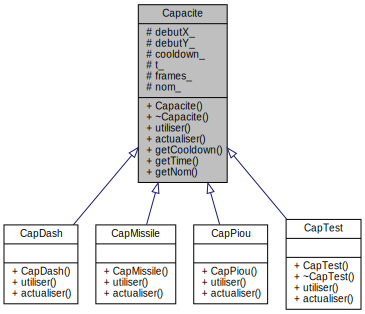
\includegraphics[width=282pt]{class_capacite__inherit__graph}
\end{center}
\end{figure}
\subsection*{Fonctions membres publiques}
\begin{DoxyCompactItemize}
\item 
\hyperlink{class_capacite_a8a1aebc5b2332e366a3f207c23b4d363}{Capacite} ()=default
\begin{DoxyCompactList}\small\item\em Constructeur. \end{DoxyCompactList}\item 
virtual \hyperlink{class_capacite_a43be1570a24a64682ff3f034330779a9}{$\sim$\+Capacite} ()=default
\begin{DoxyCompactList}\small\item\em Destructeur. \end{DoxyCompactList}\item 
virtual void \hyperlink{class_capacite_a6f5e6efda11f80ab8538e23f5bdc6e79}{utiliser} (int x, int y)=0
\begin{DoxyCompactList}\small\item\em Fonction virtuel qui active la capacite lorsqu\textquotesingle{}elle est appelée. \end{DoxyCompactList}\item 
virtual void \hyperlink{class_capacite_a924214972f385ef409031bafc0f315b7}{actualiser} (std\+::vector$<$ \hyperlink{class_projectile}{Projectile} $\ast$$>$ \&projectiles, \hyperlink{class_entite}{Entite} $\ast$vaisseau, float temps\+Ecoule)=0
\begin{DoxyCompactList}\small\item\em Fonction virtuel qui active les effets de la capacité \end{DoxyCompactList}\item 
float const \hyperlink{class_capacite_af07c1c3a2c9259a7eab270b3d8f867de}{get\+Cooldown} ()
\item 
float const \hyperlink{class_capacite_a963dd214cc53c76358b5326d9164884f}{get\+Time} ()
\item 
std\+::string const \hyperlink{class_capacite_a96218b289768ff461ffaaa0abe014a42}{get\+Nom} ()
\end{DoxyCompactItemize}
\subsection*{Attributs protégés}
\begin{DoxyCompactItemize}
\item 
int \hyperlink{class_capacite_abc3eb04129009107c0b60b03e7a3ff06}{debut\+X\+\_\+}
\item 
int \hyperlink{class_capacite_a741d48934a015c226b15e6519724e400}{debut\+Y\+\_\+}
\item 
float \hyperlink{class_capacite_aa84204be03602333d694faa14dbb693c}{cooldown\+\_\+}
\begin{DoxyCompactList}\small\item\em Position de départ. \end{DoxyCompactList}\item 
float \hyperlink{class_capacite_ade805898750e70261be4f4ced92a9063}{t\+\_\+}
\begin{DoxyCompactList}\small\item\em Temps à attendre avant de pouvoir utiliser la capacité à nouveau. \end{DoxyCompactList}\item 
unsigned int \hyperlink{class_capacite_a250c28dafd8e12b58ccfb4224329f111}{frames\+\_\+}
\begin{DoxyCompactList}\small\item\em Temps écoulé depuis la dernière activation de la compétance. \end{DoxyCompactList}\item 
std\+::string \hyperlink{class_capacite_a430472b509233086cbad1d6d8332dc8c}{nom\+\_\+}
\begin{DoxyCompactList}\small\item\em Nombre de frames écoulé depuis la dernière activation. \end{DoxyCompactList}\end{DoxyCompactItemize}


\subsection{Description détaillée}
Classe abstraite qui définit la structure générale d\textquotesingle{}une capacité, à faire hériter de chaque capacité 

Cette classe abstraite permet de définir la structure générale d\textquotesingle{}une capacité du jeu, elle doit être héritée pour chaque capacité qui est ajoutée au jeu 

\subsection{Documentation des constructeurs et destructeur}
\mbox{\Hypertarget{class_capacite_a8a1aebc5b2332e366a3f207c23b4d363}\label{class_capacite_a8a1aebc5b2332e366a3f207c23b4d363}} 
\index{Capacite@{Capacite}!Capacite@{Capacite}}
\index{Capacite@{Capacite}!Capacite@{Capacite}}
\subsubsection{\texorpdfstring{Capacite()}{Capacite()}}
{\footnotesize\ttfamily Capacite\+::\+Capacite (\begin{DoxyParamCaption}{ }\end{DoxyParamCaption})\hspace{0.3cm}{\ttfamily [default]}}



Constructeur. 

Vide \mbox{\Hypertarget{class_capacite_a43be1570a24a64682ff3f034330779a9}\label{class_capacite_a43be1570a24a64682ff3f034330779a9}} 
\index{Capacite@{Capacite}!````~Capacite@{$\sim$\+Capacite}}
\index{````~Capacite@{$\sim$\+Capacite}!Capacite@{Capacite}}
\subsubsection{\texorpdfstring{$\sim$\+Capacite()}{~Capacite()}}
{\footnotesize\ttfamily Capacite\+::$\sim$\+Capacite (\begin{DoxyParamCaption}{ }\end{DoxyParamCaption})\hspace{0.3cm}{\ttfamily [virtual]}, {\ttfamily [default]}}



Destructeur. 

Vide 

\subsection{Documentation des fonctions membres}
\mbox{\Hypertarget{class_capacite_a924214972f385ef409031bafc0f315b7}\label{class_capacite_a924214972f385ef409031bafc0f315b7}} 
\index{Capacite@{Capacite}!actualiser@{actualiser}}
\index{actualiser@{actualiser}!Capacite@{Capacite}}
\subsubsection{\texorpdfstring{actualiser()}{actualiser()}}
{\footnotesize\ttfamily Capacite\+::actualiser (\begin{DoxyParamCaption}\item[{std\+::vector$<$ \hyperlink{class_projectile}{Projectile} $\ast$$>$ \&}]{projectiles,  }\item[{\hyperlink{class_entite}{Entite} $\ast$}]{vaisseau,  }\item[{float}]{temps\+Ecoule }\end{DoxyParamCaption})\hspace{0.3cm}{\ttfamily [pure virtual]}}



Fonction virtuel qui active les effets de la capacité 


\begin{DoxyParams}{Paramètres}
{\em projectile} & Vecteur de tout les projectiles présent à l\textquotesingle{}écran \\
\hline
{\em vaisseau} & \hyperlink{class_vaisseau}{Vaisseau} qui a activé la compétance \\
\hline
{\em temp\+Ecoule} & Temps écoulé depuis la dernière boucle\\
\hline
\end{DoxyParams}
Fonction virtuel qui gère la création de projectiles et des modifications à apporter au vaisseau 

Implémenté dans \hyperlink{class_cap_piou_ae15af0a5a261349ae8462f00b6cb0d5d}{Cap\+Piou}, \hyperlink{class_cap_dash_ad4f99cef49151c1072a11af18852fa7b}{Cap\+Dash}, et \hyperlink{class_cap_test_af8e8fad88e1e4f0037eee576331d3238}{Cap\+Test}.

\mbox{\Hypertarget{class_capacite_af07c1c3a2c9259a7eab270b3d8f867de}\label{class_capacite_af07c1c3a2c9259a7eab270b3d8f867de}} 
\index{Capacite@{Capacite}!get\+Cooldown@{get\+Cooldown}}
\index{get\+Cooldown@{get\+Cooldown}!Capacite@{Capacite}}
\subsubsection{\texorpdfstring{get\+Cooldown()}{getCooldown()}}
{\footnotesize\ttfamily float const Capacite\+::get\+Cooldown (\begin{DoxyParamCaption}{ }\end{DoxyParamCaption})\hspace{0.3cm}{\ttfamily [inline]}}

\mbox{\Hypertarget{class_capacite_a96218b289768ff461ffaaa0abe014a42}\label{class_capacite_a96218b289768ff461ffaaa0abe014a42}} 
\index{Capacite@{Capacite}!get\+Nom@{get\+Nom}}
\index{get\+Nom@{get\+Nom}!Capacite@{Capacite}}
\subsubsection{\texorpdfstring{get\+Nom()}{getNom()}}
{\footnotesize\ttfamily std\+::string const Capacite\+::get\+Nom (\begin{DoxyParamCaption}{ }\end{DoxyParamCaption})\hspace{0.3cm}{\ttfamily [inline]}}

\mbox{\Hypertarget{class_capacite_a963dd214cc53c76358b5326d9164884f}\label{class_capacite_a963dd214cc53c76358b5326d9164884f}} 
\index{Capacite@{Capacite}!get\+Time@{get\+Time}}
\index{get\+Time@{get\+Time}!Capacite@{Capacite}}
\subsubsection{\texorpdfstring{get\+Time()}{getTime()}}
{\footnotesize\ttfamily float const Capacite\+::get\+Time (\begin{DoxyParamCaption}{ }\end{DoxyParamCaption})\hspace{0.3cm}{\ttfamily [inline]}}

\mbox{\Hypertarget{class_capacite_a6f5e6efda11f80ab8538e23f5bdc6e79}\label{class_capacite_a6f5e6efda11f80ab8538e23f5bdc6e79}} 
\index{Capacite@{Capacite}!utiliser@{utiliser}}
\index{utiliser@{utiliser}!Capacite@{Capacite}}
\subsubsection{\texorpdfstring{utiliser()}{utiliser()}}
{\footnotesize\ttfamily Capacite\+::utiliser (\begin{DoxyParamCaption}\item[{int}]{x,  }\item[{int}]{y }\end{DoxyParamCaption})\hspace{0.3cm}{\ttfamily [pure virtual]}}



Fonction virtuel qui active la capacite lorsqu\textquotesingle{}elle est appelée. 


\begin{DoxyParams}{Paramètres}
{\em x} & Abscisse de la postion où la capacite est utilisée \\
\hline
{\em y} & Ordonnée de la postion où la capacite est utilisée\\
\hline
\end{DoxyParams}
Fonction virtuel qui initialise la postion de départ et le timer 

Implémenté dans \hyperlink{class_cap_piou_a92f5cc3011280ad13bf3ff5e6a3c76ea}{Cap\+Piou}, \hyperlink{class_cap_dash_a82823122659ff5a87a09e9ddf0e3dabb}{Cap\+Dash}, et \hyperlink{class_cap_test_a9c85a17dec6cf78f1438b08b175f650d}{Cap\+Test}.



\subsection{Documentation des données membres}
\mbox{\Hypertarget{class_capacite_aa84204be03602333d694faa14dbb693c}\label{class_capacite_aa84204be03602333d694faa14dbb693c}} 
\index{Capacite@{Capacite}!cooldown\+\_\+@{cooldown\+\_\+}}
\index{cooldown\+\_\+@{cooldown\+\_\+}!Capacite@{Capacite}}
\subsubsection{\texorpdfstring{cooldown\+\_\+}{cooldown\_}}
{\footnotesize\ttfamily float Capacite\+::cooldown\+\_\+\hspace{0.3cm}{\ttfamily [protected]}}



Position de départ. 

\mbox{\Hypertarget{class_capacite_abc3eb04129009107c0b60b03e7a3ff06}\label{class_capacite_abc3eb04129009107c0b60b03e7a3ff06}} 
\index{Capacite@{Capacite}!debut\+X\+\_\+@{debut\+X\+\_\+}}
\index{debut\+X\+\_\+@{debut\+X\+\_\+}!Capacite@{Capacite}}
\subsubsection{\texorpdfstring{debut\+X\+\_\+}{debutX\_}}
{\footnotesize\ttfamily int Capacite\+::debut\+X\+\_\+\hspace{0.3cm}{\ttfamily [protected]}}

\mbox{\Hypertarget{class_capacite_a741d48934a015c226b15e6519724e400}\label{class_capacite_a741d48934a015c226b15e6519724e400}} 
\index{Capacite@{Capacite}!debut\+Y\+\_\+@{debut\+Y\+\_\+}}
\index{debut\+Y\+\_\+@{debut\+Y\+\_\+}!Capacite@{Capacite}}
\subsubsection{\texorpdfstring{debut\+Y\+\_\+}{debutY\_}}
{\footnotesize\ttfamily int Capacite\+::debut\+Y\+\_\+\hspace{0.3cm}{\ttfamily [protected]}}

\mbox{\Hypertarget{class_capacite_a250c28dafd8e12b58ccfb4224329f111}\label{class_capacite_a250c28dafd8e12b58ccfb4224329f111}} 
\index{Capacite@{Capacite}!frames\+\_\+@{frames\+\_\+}}
\index{frames\+\_\+@{frames\+\_\+}!Capacite@{Capacite}}
\subsubsection{\texorpdfstring{frames\+\_\+}{frames\_}}
{\footnotesize\ttfamily unsigned int Capacite\+::frames\+\_\+\hspace{0.3cm}{\ttfamily [protected]}}



Temps écoulé depuis la dernière activation de la compétance. 

\mbox{\Hypertarget{class_capacite_a430472b509233086cbad1d6d8332dc8c}\label{class_capacite_a430472b509233086cbad1d6d8332dc8c}} 
\index{Capacite@{Capacite}!nom\+\_\+@{nom\+\_\+}}
\index{nom\+\_\+@{nom\+\_\+}!Capacite@{Capacite}}
\subsubsection{\texorpdfstring{nom\+\_\+}{nom\_}}
{\footnotesize\ttfamily std\+::string Capacite\+::nom\+\_\+\hspace{0.3cm}{\ttfamily [protected]}}



Nombre de frames écoulé depuis la dernière activation. 

\mbox{\Hypertarget{class_capacite_ade805898750e70261be4f4ced92a9063}\label{class_capacite_ade805898750e70261be4f4ced92a9063}} 
\index{Capacite@{Capacite}!t\+\_\+@{t\+\_\+}}
\index{t\+\_\+@{t\+\_\+}!Capacite@{Capacite}}
\subsubsection{\texorpdfstring{t\+\_\+}{t\_}}
{\footnotesize\ttfamily float Capacite\+::t\+\_\+\hspace{0.3cm}{\ttfamily [protected]}}



Temps à attendre avant de pouvoir utiliser la capacité à nouveau. 



La documentation de cette classe a été générée à partir du fichier suivant \+:\begin{DoxyCompactItemize}
\item 
src/\+Capacites/\hyperlink{_capacite_8h}{Capacite.\+h}\end{DoxyCompactItemize}

\hypertarget{class_cap_aim_bot}{}\section{Référence de la classe Cap\+Aim\+Bot}
\label{class_cap_aim_bot}\index{Cap\+Aim\+Bot@{Cap\+Aim\+Bot}}


donne vis�e auto � un skill (missile)  




{\ttfamily \#include $<$Cap\+Aim\+Bot.\+h$>$}



Graphe d\textquotesingle{}héritage de Cap\+Aim\+Bot\+:
% FIG 0


Graphe de collaboration de Cap\+Aim\+Bot\+:
% FIG 1
\subsection*{Fonctions membres publiques}
\begin{DoxyCompactItemize}
\item 
\hyperlink{class_cap_aim_bot_ac80621e5512e382cde343c483f74c90e}{Cap\+Aim\+Bot} ()
\begin{DoxyCompactList}\small\item\em Constructeur. \end{DoxyCompactList}\item 
\hyperlink{class_cap_aim_bot_ac7deb20ca65868d6c752f137cbaea339}{$\sim$\+Cap\+Aim\+Bot} ()
\begin{DoxyCompactList}\small\item\em Destructeur. \end{DoxyCompactList}\item 
void \hyperlink{class_cap_aim_bot_a79cd2b5ebd0936e133113d5563c31396}{set\+\_\+state\+\_\+auto\+Aim\+\_\+true} (\hyperlink{class_capacite}{Capacite} \&capacite)
\begin{DoxyCompactList}\small\item\em Destructeur. \end{DoxyCompactList}\item 
void \hyperlink{class_cap_aim_bot_aaa7c76ca67faf851d511c7c46ccc8139}{set\+\_\+state\+\_\+auto\+Aim\+\_\+false} (\hyperlink{class_capacite}{Capacite} \&capacite)
\begin{DoxyCompactList}\small\item\em Destructeur. \end{DoxyCompactList}\end{DoxyCompactItemize}
\subsection*{Membres hérités additionnels}


\subsection{Description détaillée}
donne vis�e auto � un skill (missile) 

Capacit� qui permet de donner un mode vis�e auto � un autre skill du vaisseau. Niveau 1 \+: seulement le prochain tir Niveau sup�rieurs \+: plusieurs tirs

Cooldown \+: 10sec 

\subsection{Documentation des constructeurs et destructeur}
\mbox{\Hypertarget{class_cap_aim_bot_ac80621e5512e382cde343c483f74c90e}\label{class_cap_aim_bot_ac80621e5512e382cde343c483f74c90e}} 
\index{Cap\+Aim\+Bot@{Cap\+Aim\+Bot}!Cap\+Aim\+Bot@{Cap\+Aim\+Bot}}
\index{Cap\+Aim\+Bot@{Cap\+Aim\+Bot}!Cap\+Aim\+Bot@{Cap\+Aim\+Bot}}
\subsubsection{\texorpdfstring{Cap\+Aim\+Bot()}{CapAimBot()}}
{\footnotesize\ttfamily Cap\+Aim\+Bot\+::\+Cap\+Aim\+Bot (\begin{DoxyParamCaption}{ }\end{DoxyParamCaption})}



Constructeur. 

Vide \mbox{\Hypertarget{class_cap_aim_bot_ac7deb20ca65868d6c752f137cbaea339}\label{class_cap_aim_bot_ac7deb20ca65868d6c752f137cbaea339}} 
\index{Cap\+Aim\+Bot@{Cap\+Aim\+Bot}!````~Cap\+Aim\+Bot@{$\sim$\+Cap\+Aim\+Bot}}
\index{````~Cap\+Aim\+Bot@{$\sim$\+Cap\+Aim\+Bot}!Cap\+Aim\+Bot@{Cap\+Aim\+Bot}}
\subsubsection{\texorpdfstring{$\sim$\+Cap\+Aim\+Bot()}{~CapAimBot()}}
{\footnotesize\ttfamily Cap\+Aim\+Bot\+::$\sim$\+Cap\+Aim\+Bot (\begin{DoxyParamCaption}{ }\end{DoxyParamCaption})\hspace{0.3cm}{\ttfamily [inline]}}



Destructeur. 

Vide 

\subsection{Documentation des fonctions membres}
\mbox{\Hypertarget{class_cap_aim_bot_aaa7c76ca67faf851d511c7c46ccc8139}\label{class_cap_aim_bot_aaa7c76ca67faf851d511c7c46ccc8139}} 
\index{Cap\+Aim\+Bot@{Cap\+Aim\+Bot}!set\+\_\+state\+\_\+auto\+Aim\+\_\+false@{set\+\_\+state\+\_\+auto\+Aim\+\_\+false}}
\index{set\+\_\+state\+\_\+auto\+Aim\+\_\+false@{set\+\_\+state\+\_\+auto\+Aim\+\_\+false}!Cap\+Aim\+Bot@{Cap\+Aim\+Bot}}
\subsubsection{\texorpdfstring{set\+\_\+state\+\_\+auto\+Aim\+\_\+false()}{set\_state\_autoAim\_false()}}
{\footnotesize\ttfamily Cap\+Aim\+Bot\+::set\+\_\+state\+\_\+auto\+Aim\+\_\+false (\begin{DoxyParamCaption}\item[{\hyperlink{class_capacite}{Capacite} \&}]{capacite }\end{DoxyParamCaption})}



Destructeur. 

change l\textquotesingle{}état autoaim à false \mbox{\Hypertarget{class_cap_aim_bot_a79cd2b5ebd0936e133113d5563c31396}\label{class_cap_aim_bot_a79cd2b5ebd0936e133113d5563c31396}} 
\index{Cap\+Aim\+Bot@{Cap\+Aim\+Bot}!set\+\_\+state\+\_\+auto\+Aim\+\_\+true@{set\+\_\+state\+\_\+auto\+Aim\+\_\+true}}
\index{set\+\_\+state\+\_\+auto\+Aim\+\_\+true@{set\+\_\+state\+\_\+auto\+Aim\+\_\+true}!Cap\+Aim\+Bot@{Cap\+Aim\+Bot}}
\subsubsection{\texorpdfstring{set\+\_\+state\+\_\+auto\+Aim\+\_\+true()}{set\_state\_autoAim\_true()}}
{\footnotesize\ttfamily Cap\+Aim\+Bot\+::set\+\_\+state\+\_\+auto\+Aim\+\_\+true (\begin{DoxyParamCaption}\item[{\hyperlink{class_capacite}{Capacite} \&}]{capacite }\end{DoxyParamCaption})}



Destructeur. 

change l\textquotesingle{}état autoaim à true 

La documentation de cette classe a été générée à partir des fichiers suivants \+:\begin{DoxyCompactItemize}
\item 
src/\+Capacites/\hyperlink{_cap_aim_bot_8h}{Cap\+Aim\+Bot.\+h}\item 
src/\+Capacites/\hyperlink{_cap_aim_bot_8cpp}{Cap\+Aim\+Bot.\+cpp}\end{DoxyCompactItemize}

\hypertarget{class_cap_bismillah}{}\section{Référence de la classe Cap\+Bismillah}
\label{class_cap_bismillah}\index{Cap\+Bismillah@{Cap\+Bismillah}}


{\ttfamily \#include $<$Cap\+Bismillah\+Beam.\+h$>$}



Graphe d\textquotesingle{}héritage de Cap\+Bismillah\+:
% FIG 0


Graphe de collaboration de Cap\+Bismillah\+:
% FIG 1
\subsection*{Fonctions membres publiques}
\begin{DoxyCompactItemize}
\item 
\hyperlink{class_cap_bismillah_a60ffd96cf478cef48242d934380c7d7e}{Cap\+Bismillah} ()
\item 
void \hyperlink{class_cap_bismillah_a9c3b48cacee26d055f24bf05f669cfca}{utiliser} (int x, int y)
\begin{DoxyCompactList}\small\item\em Fonction virtuel qui active la capacite lorsqu\textquotesingle{}elle est appelée. \end{DoxyCompactList}\item 
void \hyperlink{class_cap_bismillah_aef9579d9a4ee46cc92873ceb6440560a}{actualiser} (std\+::vector$<$ \hyperlink{class_projectile}{Projectile} $\ast$$>$ \&projectiles, \hyperlink{class_entite}{Entite} \&vaisseau, float temps\+Ecoule)
\begin{DoxyCompactList}\small\item\em Fonction virtuel qui active les effets de la capacité \end{DoxyCompactList}\end{DoxyCompactItemize}
\subsection*{Membres hérités additionnels}


\subsection{Documentation des constructeurs et destructeur}
\mbox{\Hypertarget{class_cap_bismillah_a60ffd96cf478cef48242d934380c7d7e}\label{class_cap_bismillah_a60ffd96cf478cef48242d934380c7d7e}} 
\index{Cap\+Bismillah@{Cap\+Bismillah}!Cap\+Bismillah@{Cap\+Bismillah}}
\index{Cap\+Bismillah@{Cap\+Bismillah}!Cap\+Bismillah@{Cap\+Bismillah}}
\subsubsection{\texorpdfstring{Cap\+Bismillah()}{CapBismillah()}}
{\footnotesize\ttfamily Cap\+Bismillah\+::\+Cap\+Bismillah (\begin{DoxyParamCaption}{ }\end{DoxyParamCaption})}



\subsection{Documentation des fonctions membres}
\mbox{\Hypertarget{class_cap_bismillah_aef9579d9a4ee46cc92873ceb6440560a}\label{class_cap_bismillah_aef9579d9a4ee46cc92873ceb6440560a}} 
\index{Cap\+Bismillah@{Cap\+Bismillah}!actualiser@{actualiser}}
\index{actualiser@{actualiser}!Cap\+Bismillah@{Cap\+Bismillah}}
\subsubsection{\texorpdfstring{actualiser()}{actualiser()}}
{\footnotesize\ttfamily void Cap\+Bismillah\+::actualiser (\begin{DoxyParamCaption}\item[{std\+::vector$<$ \hyperlink{class_projectile}{Projectile} $\ast$$>$ \&}]{projectiles,  }\item[{\hyperlink{class_entite}{Entite} \&}]{vaisseau,  }\item[{float}]{temps\+Ecoule }\end{DoxyParamCaption})\hspace{0.3cm}{\ttfamily [virtual]}}



Fonction virtuel qui active les effets de la capacité 


\begin{DoxyParams}{Paramètres}
{\em projectile} & Vecteur de tout les projectiles présent à l\textquotesingle{}écran \\
\hline
{\em vaisseau} & \hyperlink{class_vaisseau}{Vaisseau} qui a activé la compétence \\
\hline
{\em temp\+Ecoule} & Temps écoulé depuis la dernière boucle\\
\hline
\end{DoxyParams}
Fonction virtuel qui gère la création de projectiles et des modifications à apporter au vaisseau 

Implémente \hyperlink{class_capacite_a75c9621d7a704fedb10ad29c6a697d64}{Capacite}.

\mbox{\Hypertarget{class_cap_bismillah_a9c3b48cacee26d055f24bf05f669cfca}\label{class_cap_bismillah_a9c3b48cacee26d055f24bf05f669cfca}} 
\index{Cap\+Bismillah@{Cap\+Bismillah}!utiliser@{utiliser}}
\index{utiliser@{utiliser}!Cap\+Bismillah@{Cap\+Bismillah}}
\subsubsection{\texorpdfstring{utiliser()}{utiliser()}}
{\footnotesize\ttfamily void Cap\+Bismillah\+::utiliser (\begin{DoxyParamCaption}\item[{int}]{x,  }\item[{int}]{y }\end{DoxyParamCaption})\hspace{0.3cm}{\ttfamily [virtual]}}



Fonction virtuel qui active la capacite lorsqu\textquotesingle{}elle est appelée. 


\begin{DoxyParams}{Paramètres}
{\em x} & Abscisse de la position où la capacite est utilisée \\
\hline
{\em y} & Ordonnée de la position où la capacite est utilisée\\
\hline
\end{DoxyParams}
Fonction virtuel qui initialise la position de départ et le timer 

Implémente \hyperlink{class_capacite_a6f5e6efda11f80ab8538e23f5bdc6e79}{Capacite}.



La documentation de cette classe a été générée à partir des fichiers suivants \+:\begin{DoxyCompactItemize}
\item 
src/\+Capacites/\hyperlink{_cap_bismillah_beam_8h}{Cap\+Bismillah\+Beam.\+h}\item 
src/\+Capacites/\hyperlink{_cap_bismillah_beam_8cpp}{Cap\+Bismillah\+Beam.\+cpp}\end{DoxyCompactItemize}

\hypertarget{class_cap_boing}{}\section{Cap\+Boing Class Reference}
\label{class_cap_boing}\index{Cap\+Boing@{Cap\+Boing}}


Classe Capacité de test.  




{\ttfamily \#include $<$Cap\+Boing.\+h$>$}

Inheritance diagram for Cap\+Boing\+:\begin{figure}[H]
\begin{center}
\leavevmode
\includegraphics[height=2.000000cm]{class_cap_boing}
\end{center}
\end{figure}
\subsection*{Public Member Functions}
\begin{DoxyCompactItemize}
\item 
\mbox{\hyperlink{class_cap_boing_a9d315f24e4dfa2406956a9c53624d2ec}{Cap\+Boing}} (\mbox{\hyperlink{class_ecran}{Ecran}} \&ecran, const std\+::weak\+\_\+ptr$<$ \mbox{\hyperlink{class_entite}{Entite}} $>$ \&lanceur)
\begin{DoxyCompactList}\small\item\em Constructeur. \end{DoxyCompactList}\item 
\mbox{\hyperlink{class_cap_boing_a7f90c88c46fa87ff4c0fb66708648f96}{$\sim$\+Cap\+Boing}} () override=default
\begin{DoxyCompactList}\small\item\em Destructeur. \end{DoxyCompactList}\item 
void \mbox{\hyperlink{class_cap_boing_a879dfeba930a0be60873ef3403a35eb1}{utiliser}} (\mbox{\hyperlink{def__type_8h_a87980cd8ee9533e561a73e8bbc728188}{proj\+\_\+container}} \&projectiles) override
\begin{DoxyCompactList}\small\item\em Active la capacite. \end{DoxyCompactList}\item 
void \mbox{\hyperlink{class_cap_boing_a2bf6f58f93ff52263cf9926e4d91c239}{actualiser}} (\mbox{\hyperlink{def__type_8h_a87980cd8ee9533e561a73e8bbc728188}{proj\+\_\+container}} \&projectiles) override
\begin{DoxyCompactList}\small\item\em Active les effets de la capacité \end{DoxyCompactList}\end{DoxyCompactItemize}
\subsection*{Additional Inherited Members}


\subsection{Detailed Description}
Classe Capacité de test. 

Capacité qui créé 4 \mbox{\hyperlink{class_proj_boing}{Proj\+Boing}} à la position du lanceur Nom \+: Attaque Test Cooldown \+: 1000 ms 

\subsection{Constructor \& Destructor Documentation}
\mbox{\Hypertarget{class_cap_boing_a9d315f24e4dfa2406956a9c53624d2ec}\label{class_cap_boing_a9d315f24e4dfa2406956a9c53624d2ec}} 
\index{Cap\+Boing@{Cap\+Boing}!Cap\+Boing@{Cap\+Boing}}
\index{Cap\+Boing@{Cap\+Boing}!Cap\+Boing@{Cap\+Boing}}
\subsubsection{\texorpdfstring{Cap\+Boing()}{CapBoing()}}
{\footnotesize\ttfamily Cap\+Boing\+::\+Cap\+Boing (\begin{DoxyParamCaption}\item[{\mbox{\hyperlink{class_ecran}{Ecran}} \&}]{ecran,  }\item[{const std\+::weak\+\_\+ptr$<$ \mbox{\hyperlink{class_entite}{Entite}} $>$ \&}]{lanceur }\end{DoxyParamCaption})}



Constructeur. 

Initialisation de la capacité \mbox{\Hypertarget{class_cap_boing_a7f90c88c46fa87ff4c0fb66708648f96}\label{class_cap_boing_a7f90c88c46fa87ff4c0fb66708648f96}} 
\index{Cap\+Boing@{Cap\+Boing}!````~Cap\+Boing@{$\sim$\+Cap\+Boing}}
\index{````~Cap\+Boing@{$\sim$\+Cap\+Boing}!Cap\+Boing@{Cap\+Boing}}
\subsubsection{\texorpdfstring{$\sim$\+Cap\+Boing()}{~CapBoing()}}
{\footnotesize\ttfamily Cap\+Boing\+::$\sim$\+Cap\+Boing (\begin{DoxyParamCaption}{ }\end{DoxyParamCaption})\hspace{0.3cm}{\ttfamily [override]}, {\ttfamily [default]}}



Destructeur. 

Vide 

\subsection{Member Function Documentation}
\mbox{\Hypertarget{class_cap_boing_a2bf6f58f93ff52263cf9926e4d91c239}\label{class_cap_boing_a2bf6f58f93ff52263cf9926e4d91c239}} 
\index{Cap\+Boing@{Cap\+Boing}!actualiser@{actualiser}}
\index{actualiser@{actualiser}!Cap\+Boing@{Cap\+Boing}}
\subsubsection{\texorpdfstring{actualiser()}{actualiser()}}
{\footnotesize\ttfamily Cap\+Boing\+::actualiser (\begin{DoxyParamCaption}\item[{\mbox{\hyperlink{def__type_8h_a87980cd8ee9533e561a73e8bbc728188}{proj\+\_\+container}} \&}]{projectiles }\end{DoxyParamCaption})\hspace{0.3cm}{\ttfamily [override]}, {\ttfamily [virtual]}}



Active les effets de la capacité 


\begin{DoxyParams}{Parameters}
{\em projectile} & Vecteur de tout les projectiles présent à l\textquotesingle{}écran \\
\hline
{\em vaisseau} & \mbox{\hyperlink{class_vaisseau}{Vaisseau}} qui a activé la compétence\\
\hline
\end{DoxyParams}
Créer 4 \mbox{\hyperlink{class_proj_boing}{Proj\+Boing}} toutes les 5 frames Actualise le timer 

Implements \mbox{\hyperlink{class_capacite_a85355aeb1d4acc049ed97da177acbd5f}{Capacite}}.

\mbox{\Hypertarget{class_cap_boing_a879dfeba930a0be60873ef3403a35eb1}\label{class_cap_boing_a879dfeba930a0be60873ef3403a35eb1}} 
\index{Cap\+Boing@{Cap\+Boing}!utiliser@{utiliser}}
\index{utiliser@{utiliser}!Cap\+Boing@{Cap\+Boing}}
\subsubsection{\texorpdfstring{utiliser()}{utiliser()}}
{\footnotesize\ttfamily Cap\+Boing\+::utiliser (\begin{DoxyParamCaption}\item[{\mbox{\hyperlink{def__type_8h_a87980cd8ee9533e561a73e8bbc728188}{proj\+\_\+container}} \&}]{projectiles }\end{DoxyParamCaption})\hspace{0.3cm}{\ttfamily [override]}, {\ttfamily [virtual]}}



Active la capacite. 


\begin{DoxyParams}{Parameters}
{\em x} & Abscisse de la position où la capacite est utilisée \\
\hline
{\em y} & Ordonnée de la position où la capacite est utilisée\\
\hline
\end{DoxyParams}
Fonction Initialise la position de départ et le timer 

Implements \mbox{\hyperlink{class_capacite_abac1434e2ac3ecc9e5afdafd9a7a4bed}{Capacite}}.



The documentation for this class was generated from the following files\+:\begin{DoxyCompactItemize}
\item 
src/\+Capacites/\mbox{\hyperlink{_cap_boing_8h}{Cap\+Boing.\+h}}\item 
src/\+Capacites/\mbox{\hyperlink{_cap_boing_8cpp}{Cap\+Boing.\+cpp}}\end{DoxyCompactItemize}

\hypertarget{class_cap_bouclier_rond}{}\section{Cap\+Bouclier\+Rond Class Reference}
\label{class_cap_bouclier_rond}\index{Cap\+Bouclier\+Rond@{Cap\+Bouclier\+Rond}}


bouclier circulaire avec x PB  




{\ttfamily \#include $<$Cap\+Bouclier\+Rond.\+h$>$}

Inheritance diagram for Cap\+Bouclier\+Rond\+:\begin{figure}[H]
\begin{center}
\leavevmode
\includegraphics[height=2.000000cm]{class_cap_bouclier_rond}
\end{center}
\end{figure}
\subsection*{Public Member Functions}
\begin{DoxyCompactItemize}
\item 
\mbox{\hyperlink{class_cap_bouclier_rond_a371bae2937bafb1cef7e1867a93ba8a1}{Cap\+Bouclier\+Rond}} (\mbox{\hyperlink{class_ecran}{Ecran}} \&ecran, const std\+::weak\+\_\+ptr$<$ \mbox{\hyperlink{class_entite}{Entite}} $>$ \&lanceur)
\begin{DoxyCompactList}\small\item\em Constructeur. \end{DoxyCompactList}\item 
void \mbox{\hyperlink{class_cap_bouclier_rond_ae420337d3d5c5ec2e5a4a0cafa8f69ad}{utiliser}} (\mbox{\hyperlink{def__type_8h_a87980cd8ee9533e561a73e8bbc728188}{proj\+\_\+container}} \&projectiles) override
\begin{DoxyCompactList}\small\item\em Fonction virtuel qui active la capacite lorsqu\textquotesingle{}elle est appelée. \end{DoxyCompactList}\item 
void \mbox{\hyperlink{class_cap_bouclier_rond_ab664fc0b17a849d606d1a1085f2095c8}{actualiser}} (\mbox{\hyperlink{def__type_8h_a87980cd8ee9533e561a73e8bbc728188}{proj\+\_\+container}} \&projectiles) override
\begin{DoxyCompactList}\small\item\em Fonction virtuel qui active les effets de la capacité \end{DoxyCompactList}\end{DoxyCompactItemize}
\subsection*{Additional Inherited Members}


\subsection{Detailed Description}
bouclier circulaire avec x PB 

Donne un bouclier circulaire qui entoure le vaisseau. Il est supprimé après un certain temps ( s sec) ou si ses (pb) PB tombent à zéro. Le bouclier est un projectile. Niveau 1 \+: Niveau supérieurs (idées) \+: augmente PB, temps de stase, réduit CD

Cooldown \+: 10sec 

\subsection{Constructor \& Destructor Documentation}
\mbox{\Hypertarget{class_cap_bouclier_rond_a371bae2937bafb1cef7e1867a93ba8a1}\label{class_cap_bouclier_rond_a371bae2937bafb1cef7e1867a93ba8a1}} 
\index{Cap\+Bouclier\+Rond@{Cap\+Bouclier\+Rond}!Cap\+Bouclier\+Rond@{Cap\+Bouclier\+Rond}}
\index{Cap\+Bouclier\+Rond@{Cap\+Bouclier\+Rond}!Cap\+Bouclier\+Rond@{Cap\+Bouclier\+Rond}}
\subsubsection{\texorpdfstring{Cap\+Bouclier\+Rond()}{CapBouclierRond()}}
{\footnotesize\ttfamily Cap\+Bouclier\+Rond\+::\+Cap\+Bouclier\+Rond (\begin{DoxyParamCaption}\item[{\mbox{\hyperlink{class_ecran}{Ecran}} \&}]{ecran,  }\item[{const std\+::weak\+\_\+ptr$<$ \mbox{\hyperlink{class_entite}{Entite}} $>$ \&}]{lanceur }\end{DoxyParamCaption})}



Constructeur. 


\begin{DoxyParams}{Parameters}
{\em niveau} & niveau de la capacité \\
\hline
{\em Entite\+\_\+liee\+\_\+} & \mbox{\hyperlink{class_entite}{Entite}} à laquelle s\textquotesingle{}applique le bouclier\\
\hline
\end{DoxyParams}
Initialisation 

\subsection{Member Function Documentation}
\mbox{\Hypertarget{class_cap_bouclier_rond_ab664fc0b17a849d606d1a1085f2095c8}\label{class_cap_bouclier_rond_ab664fc0b17a849d606d1a1085f2095c8}} 
\index{Cap\+Bouclier\+Rond@{Cap\+Bouclier\+Rond}!actualiser@{actualiser}}
\index{actualiser@{actualiser}!Cap\+Bouclier\+Rond@{Cap\+Bouclier\+Rond}}
\subsubsection{\texorpdfstring{actualiser()}{actualiser()}}
{\footnotesize\ttfamily void Cap\+Bouclier\+Rond\+::actualiser (\begin{DoxyParamCaption}\item[{\mbox{\hyperlink{def__type_8h_a87980cd8ee9533e561a73e8bbc728188}{proj\+\_\+container}} \&}]{projectiles }\end{DoxyParamCaption})\hspace{0.3cm}{\ttfamily [override]}, {\ttfamily [virtual]}}



Fonction virtuel qui active les effets de la capacité 


\begin{DoxyParams}{Parameters}
{\em projectile} & Vecteur de shared\+\_\+ptr sur tous les projectiles présent à l\textquotesingle{}écran\\
\hline
\end{DoxyParams}
Fonction virtuelle qui gère la création de projectiles et des modifications à apporter au vaisseau 

Implements \mbox{\hyperlink{class_capacite_a85355aeb1d4acc049ed97da177acbd5f}{Capacite}}.

\mbox{\Hypertarget{class_cap_bouclier_rond_ae420337d3d5c5ec2e5a4a0cafa8f69ad}\label{class_cap_bouclier_rond_ae420337d3d5c5ec2e5a4a0cafa8f69ad}} 
\index{Cap\+Bouclier\+Rond@{Cap\+Bouclier\+Rond}!utiliser@{utiliser}}
\index{utiliser@{utiliser}!Cap\+Bouclier\+Rond@{Cap\+Bouclier\+Rond}}
\subsubsection{\texorpdfstring{utiliser()}{utiliser()}}
{\footnotesize\ttfamily void Cap\+Bouclier\+Rond\+::utiliser (\begin{DoxyParamCaption}\item[{\mbox{\hyperlink{def__type_8h_a87980cd8ee9533e561a73e8bbc728188}{proj\+\_\+container}} \&}]{projectile }\end{DoxyParamCaption})\hspace{0.3cm}{\ttfamily [override]}, {\ttfamily [virtual]}}



Fonction virtuel qui active la capacite lorsqu\textquotesingle{}elle est appelée. 

Fonction virtuel qui initialise la position de départ et le timer 

Implements \mbox{\hyperlink{class_capacite_abac1434e2ac3ecc9e5afdafd9a7a4bed}{Capacite}}.



The documentation for this class was generated from the following files\+:\begin{DoxyCompactItemize}
\item 
src/\+Capacites/\mbox{\hyperlink{_cap_bouclier_rond_8h}{Cap\+Bouclier\+Rond.\+h}}\item 
src/\+Capacites/\mbox{\hyperlink{_cap_bouclier_rond_8cpp}{Cap\+Bouclier\+Rond.\+cpp}}\end{DoxyCompactItemize}

\hypertarget{class_cap_dash}{}\section{Référence de la classe Cap\+Dash}
\label{class_cap_dash}\index{Cap\+Dash@{Cap\+Dash}}


{\ttfamily \#include $<$Cap\+Dash.\+h$>$}



Graphe d\textquotesingle{}héritage de Cap\+Dash\+:
\nopagebreak
\begin{figure}[H]
\begin{center}
\leavevmode
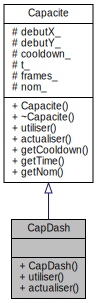
\includegraphics[width=138pt]{class_cap_dash__inherit__graph}
\end{center}
\end{figure}


Graphe de collaboration de Cap\+Dash\+:
\nopagebreak
\begin{figure}[H]
\begin{center}
\leavevmode
\includegraphics[width=138pt]{class_cap_dash__coll__graph}
\end{center}
\end{figure}
\subsection*{Fonctions membres publiques}
\begin{DoxyCompactItemize}
\item 
\hyperlink{class_cap_dash_ac38287e31284b6b5ac8add730830bfed}{Cap\+Dash} ()
\item 
\hyperlink{class_cap_dash_aa935262b9ebdaf197294aba7211663cc}{$\sim$\+Cap\+Dash} ()
\item 
void \hyperlink{class_cap_dash_ada59ecb62d2c18f6bb6b4acf28a2da93}{utiliser} (int x, int y)
\item 
void \hyperlink{class_cap_dash_a886522c648db49b81c330737ad96a517}{actualiser} (std\+::vector$<$ \hyperlink{class_projectile}{Projectile} $\ast$$>$ \&projectiles, \hyperlink{class_entite}{Entite} $\ast$vaisseau)
\end{DoxyCompactItemize}
\subsection*{Membres hérités additionnels}


\subsection{Documentation des constructeurs et destructeur}
\mbox{\Hypertarget{class_cap_dash_ac38287e31284b6b5ac8add730830bfed}\label{class_cap_dash_ac38287e31284b6b5ac8add730830bfed}} 
\index{Cap\+Dash@{Cap\+Dash}!Cap\+Dash@{Cap\+Dash}}
\index{Cap\+Dash@{Cap\+Dash}!Cap\+Dash@{Cap\+Dash}}
\subsubsection{\texorpdfstring{Cap\+Dash()}{CapDash()}}
{\footnotesize\ttfamily Cap\+Dash\+::\+Cap\+Dash (\begin{DoxyParamCaption}{ }\end{DoxyParamCaption})}

\mbox{\Hypertarget{class_cap_dash_aa935262b9ebdaf197294aba7211663cc}\label{class_cap_dash_aa935262b9ebdaf197294aba7211663cc}} 
\index{Cap\+Dash@{Cap\+Dash}!````~Cap\+Dash@{$\sim$\+Cap\+Dash}}
\index{````~Cap\+Dash@{$\sim$\+Cap\+Dash}!Cap\+Dash@{Cap\+Dash}}
\subsubsection{\texorpdfstring{$\sim$\+Cap\+Dash()}{~CapDash()}}
{\footnotesize\ttfamily Cap\+Dash\+::$\sim$\+Cap\+Dash (\begin{DoxyParamCaption}{ }\end{DoxyParamCaption})}



\subsection{Documentation des fonctions membres}
\mbox{\Hypertarget{class_cap_dash_a886522c648db49b81c330737ad96a517}\label{class_cap_dash_a886522c648db49b81c330737ad96a517}} 
\index{Cap\+Dash@{Cap\+Dash}!actualiser@{actualiser}}
\index{actualiser@{actualiser}!Cap\+Dash@{Cap\+Dash}}
\subsubsection{\texorpdfstring{actualiser()}{actualiser()}}
{\footnotesize\ttfamily void Cap\+Dash\+::actualiser (\begin{DoxyParamCaption}\item[{std\+::vector$<$ \hyperlink{class_projectile}{Projectile} $\ast$$>$ \&}]{projectiles,  }\item[{\hyperlink{class_entite}{Entite} $\ast$}]{vaisseau }\end{DoxyParamCaption})\hspace{0.3cm}{\ttfamily [virtual]}}



Implémente \hyperlink{class_capacite_a7d4e86c20cd198960f25c0eb443148fe}{Capacite}.

\mbox{\Hypertarget{class_cap_dash_ada59ecb62d2c18f6bb6b4acf28a2da93}\label{class_cap_dash_ada59ecb62d2c18f6bb6b4acf28a2da93}} 
\index{Cap\+Dash@{Cap\+Dash}!utiliser@{utiliser}}
\index{utiliser@{utiliser}!Cap\+Dash@{Cap\+Dash}}
\subsubsection{\texorpdfstring{utiliser()}{utiliser()}}
{\footnotesize\ttfamily void Cap\+Dash\+::utiliser (\begin{DoxyParamCaption}\item[{int}]{x,  }\item[{int}]{y }\end{DoxyParamCaption})\hspace{0.3cm}{\ttfamily [virtual]}}



Implémente \hyperlink{class_capacite_a4d4f643987fcc2168567bf28a36ea418}{Capacite}.



La documentation de cette classe a été générée à partir des fichiers suivants \+:\begin{DoxyCompactItemize}
\item 
src/\+Capacites/\hyperlink{_cap_dash_8h}{Cap\+Dash.\+h}\item 
src/\+Capacites/\hyperlink{_cap_dash_8cpp}{Cap\+Dash.\+cpp}\end{DoxyCompactItemize}

\hypertarget{class_cap_missile}{}\section{Cap\+Missile Class Reference}
\label{class_cap_missile}\index{Cap\+Missile@{Cap\+Missile}}


Classe Capacité de base.  




{\ttfamily \#include $<$Cap\+Missile.\+h$>$}

Inheritance diagram for Cap\+Missile\+:\begin{figure}[H]
\begin{center}
\leavevmode
\includegraphics[height=2.000000cm]{class_cap_missile}
\end{center}
\end{figure}
\subsection*{Public Member Functions}
\begin{DoxyCompactItemize}
\item 
\mbox{\hyperlink{class_cap_missile_a6cb9e154556aab9d8a7f41bd7d7cfdbc}{Cap\+Missile}} (\mbox{\hyperlink{class_ecran}{Ecran}} \&ecran, const std\+::weak\+\_\+ptr$<$ \mbox{\hyperlink{class_entite}{Entite}} $>$ \&lanceur)
\item 
void \mbox{\hyperlink{class_cap_missile_a8972a92894ca15903563ec41bc63c6ef}{utiliser}} (\mbox{\hyperlink{def__type_8h_a87980cd8ee9533e561a73e8bbc728188}{proj\+\_\+container}} \&projectiles) override
\begin{DoxyCompactList}\small\item\em Active la capacite. \end{DoxyCompactList}\item 
void \mbox{\hyperlink{class_cap_missile_ae61423876aa92fc8e2555b1b856a7443}{actualiser}} (\mbox{\hyperlink{def__type_8h_a87980cd8ee9533e561a73e8bbc728188}{proj\+\_\+container}} \&projectiles) override
\begin{DoxyCompactList}\small\item\em Active les effets de la capacité \end{DoxyCompactList}\end{DoxyCompactItemize}
\subsection*{Additional Inherited Members}


\subsection{Detailed Description}
Classe Capacité de base. 

Capacité qui créé 1 \mbox{\hyperlink{class_proj_missile}{Proj\+Missile}} à la position du lanceur Nom \+: Missile Cooldown \+: 5000 ms 

\subsection{Constructor \& Destructor Documentation}
\mbox{\Hypertarget{class_cap_missile_a6cb9e154556aab9d8a7f41bd7d7cfdbc}\label{class_cap_missile_a6cb9e154556aab9d8a7f41bd7d7cfdbc}} 
\index{Cap\+Missile@{Cap\+Missile}!Cap\+Missile@{Cap\+Missile}}
\index{Cap\+Missile@{Cap\+Missile}!Cap\+Missile@{Cap\+Missile}}
\subsubsection{\texorpdfstring{Cap\+Missile()}{CapMissile()}}
{\footnotesize\ttfamily Cap\+Missile\+::\+Cap\+Missile (\begin{DoxyParamCaption}\item[{\mbox{\hyperlink{class_ecran}{Ecran}} \&}]{ecran,  }\item[{const std\+::weak\+\_\+ptr$<$ \mbox{\hyperlink{class_entite}{Entite}} $>$ \&}]{lanceur }\end{DoxyParamCaption})}



\subsection{Member Function Documentation}
\mbox{\Hypertarget{class_cap_missile_ae61423876aa92fc8e2555b1b856a7443}\label{class_cap_missile_ae61423876aa92fc8e2555b1b856a7443}} 
\index{Cap\+Missile@{Cap\+Missile}!actualiser@{actualiser}}
\index{actualiser@{actualiser}!Cap\+Missile@{Cap\+Missile}}
\subsubsection{\texorpdfstring{actualiser()}{actualiser()}}
{\footnotesize\ttfamily Cap\+Missile\+::actualiser (\begin{DoxyParamCaption}\item[{\mbox{\hyperlink{def__type_8h_a87980cd8ee9533e561a73e8bbc728188}{proj\+\_\+container}} \&}]{projectiles }\end{DoxyParamCaption})\hspace{0.3cm}{\ttfamily [override]}, {\ttfamily [virtual]}}



Active les effets de la capacité 

Créer 1 \mbox{\hyperlink{class_proj_piou}{Proj\+Piou}} à l\textquotesingle{}activation Actualise le timer 
\begin{DoxyParams}{Parameters}
{\em projectile} & Vecteur de tout les projectiles présent à l\textquotesingle{}écran \\
\hline
{\em vaisseau} & \mbox{\hyperlink{class_vaisseau}{Vaisseau}} qui a activé la compétence \\
\hline
\end{DoxyParams}


Implements \mbox{\hyperlink{class_capacite_a85355aeb1d4acc049ed97da177acbd5f}{Capacite}}.

\mbox{\Hypertarget{class_cap_missile_a8972a92894ca15903563ec41bc63c6ef}\label{class_cap_missile_a8972a92894ca15903563ec41bc63c6ef}} 
\index{Cap\+Missile@{Cap\+Missile}!utiliser@{utiliser}}
\index{utiliser@{utiliser}!Cap\+Missile@{Cap\+Missile}}
\subsubsection{\texorpdfstring{utiliser()}{utiliser()}}
{\footnotesize\ttfamily Cap\+Missile\+::utiliser (\begin{DoxyParamCaption}\item[{\mbox{\hyperlink{def__type_8h_a87980cd8ee9533e561a73e8bbc728188}{proj\+\_\+container}} \&}]{projectiles }\end{DoxyParamCaption})\hspace{0.3cm}{\ttfamily [override]}, {\ttfamily [virtual]}}



Active la capacite. 


\begin{DoxyParams}{Parameters}
{\em x} & Abscisse de la position où la capacite est utilisée \\
\hline
{\em y} & Ordonnée de la position où la capacite est utilisée\\
\hline
\end{DoxyParams}
Fonction Initialise la position de départ et le timer 

Implements \mbox{\hyperlink{class_capacite_abac1434e2ac3ecc9e5afdafd9a7a4bed}{Capacite}}.



The documentation for this class was generated from the following files\+:\begin{DoxyCompactItemize}
\item 
src/\+Capacites/\mbox{\hyperlink{_cap_missile_8h}{Cap\+Missile.\+h}}\item 
src/\+Capacites/\mbox{\hyperlink{_cap_missile_8cpp}{Cap\+Missile.\+cpp}}\end{DoxyCompactItemize}

\hypertarget{class_cap_piou}{}\section{Référence de la classe Cap\+Piou}
\label{class_cap_piou}\index{Cap\+Piou@{Cap\+Piou}}


{\ttfamily \#include $<$Cap\+Piou.\+h$>$}



Graphe d\textquotesingle{}héritage de Cap\+Piou\+:\nopagebreak
\begin{figure}[H]
\begin{center}
\leavevmode
\includegraphics[width=136pt]{class_cap_piou__inherit__graph}
\end{center}
\end{figure}


Graphe de collaboration de Cap\+Piou\+:\nopagebreak
\begin{figure}[H]
\begin{center}
\leavevmode
\includegraphics[width=136pt]{class_cap_piou__coll__graph}
\end{center}
\end{figure}
\subsection*{Fonctions membres publiques}
\begin{DoxyCompactItemize}
\item 
\hyperlink{class_cap_piou_aa2ed61fb1313a447cf8444399001750d}{Cap\+Piou} ()
\item 
\hyperlink{class_cap_piou_a35d7e0b0c14d6a6e01ba0a053a8a60bd}{$\sim$\+Cap\+Piou} ()
\item 
void \hyperlink{class_cap_piou_a20ed7a993ce209a3df246f655f107f22}{utiliser} (int x, int y)
\item 
void \hyperlink{class_cap_piou_aabdcaa253f10db2bca12e750005485fc}{actualiser} (std\+::vector$<$ \hyperlink{class_projectile}{Projectile} $\ast$$>$ \&projectiles, \hyperlink{class_entite}{Entite} $\ast$vaisseau)
\end{DoxyCompactItemize}
\subsection*{Membres hérités additionnels}


\subsection{Documentation des constructeurs et destructeur}
\mbox{\Hypertarget{class_cap_piou_aa2ed61fb1313a447cf8444399001750d}\label{class_cap_piou_aa2ed61fb1313a447cf8444399001750d}} 
\index{Cap\+Piou@{Cap\+Piou}!Cap\+Piou@{Cap\+Piou}}
\index{Cap\+Piou@{Cap\+Piou}!Cap\+Piou@{Cap\+Piou}}
\subsubsection{\texorpdfstring{Cap\+Piou()}{CapPiou()}}
{\footnotesize\ttfamily Cap\+Piou\+::\+Cap\+Piou (\begin{DoxyParamCaption}{ }\end{DoxyParamCaption})}

\mbox{\Hypertarget{class_cap_piou_a35d7e0b0c14d6a6e01ba0a053a8a60bd}\label{class_cap_piou_a35d7e0b0c14d6a6e01ba0a053a8a60bd}} 
\index{Cap\+Piou@{Cap\+Piou}!````~Cap\+Piou@{$\sim$\+Cap\+Piou}}
\index{````~Cap\+Piou@{$\sim$\+Cap\+Piou}!Cap\+Piou@{Cap\+Piou}}
\subsubsection{\texorpdfstring{$\sim$\+Cap\+Piou()}{~CapPiou()}}
{\footnotesize\ttfamily Cap\+Piou\+::$\sim$\+Cap\+Piou (\begin{DoxyParamCaption}{ }\end{DoxyParamCaption})}



\subsection{Documentation des fonctions membres}
\mbox{\Hypertarget{class_cap_piou_aabdcaa253f10db2bca12e750005485fc}\label{class_cap_piou_aabdcaa253f10db2bca12e750005485fc}} 
\index{Cap\+Piou@{Cap\+Piou}!actualiser@{actualiser}}
\index{actualiser@{actualiser}!Cap\+Piou@{Cap\+Piou}}
\subsubsection{\texorpdfstring{actualiser()}{actualiser()}}
{\footnotesize\ttfamily void Cap\+Piou\+::actualiser (\begin{DoxyParamCaption}\item[{std\+::vector$<$ \hyperlink{class_projectile}{Projectile} $\ast$$>$ \&}]{projectiles,  }\item[{\hyperlink{class_entite}{Entite} $\ast$}]{vaisseau }\end{DoxyParamCaption})\hspace{0.3cm}{\ttfamily [virtual]}}



Implémente \hyperlink{class_capacite_a7d4e86c20cd198960f25c0eb443148fe}{Capacite}.

\mbox{\Hypertarget{class_cap_piou_a20ed7a993ce209a3df246f655f107f22}\label{class_cap_piou_a20ed7a993ce209a3df246f655f107f22}} 
\index{Cap\+Piou@{Cap\+Piou}!utiliser@{utiliser}}
\index{utiliser@{utiliser}!Cap\+Piou@{Cap\+Piou}}
\subsubsection{\texorpdfstring{utiliser()}{utiliser()}}
{\footnotesize\ttfamily void Cap\+Piou\+::utiliser (\begin{DoxyParamCaption}\item[{int}]{x,  }\item[{int}]{y }\end{DoxyParamCaption})\hspace{0.3cm}{\ttfamily [virtual]}}



Implémente \hyperlink{class_capacite_a4d4f643987fcc2168567bf28a36ea418}{Capacite}.



La documentation de cette classe a été générée à partir des fichiers suivants \+:\begin{DoxyCompactItemize}
\item 
src/\+Capacites/\hyperlink{_cap_piou_8h}{Cap\+Piou.\+h}\item 
src/\+Capacites/\hyperlink{_cap_piou_8cpp}{Cap\+Piou.\+cpp}\end{DoxyCompactItemize}

\hypertarget{structcase_insensitive_compare}{}\section{case\+Insensitive\+Compare Struct Reference}
\label{structcase_insensitive_compare}\index{case\+Insensitive\+Compare@{case\+Insensitive\+Compare}}


{\ttfamily \#include $<$Chargeur.\+h$>$}

\subsection*{Public Member Functions}
\begin{DoxyCompactItemize}
\item 
bool \mbox{\hyperlink{structcase_insensitive_compare_a3c5c719e651a350a54ccae077eda5d20}{operator()}} (const std\+::string \&a, const std\+::string \&b) const
\end{DoxyCompactItemize}


\subsection{Member Function Documentation}
\mbox{\Hypertarget{structcase_insensitive_compare_a3c5c719e651a350a54ccae077eda5d20}\label{structcase_insensitive_compare_a3c5c719e651a350a54ccae077eda5d20}} 
\index{case\+Insensitive\+Compare@{case\+Insensitive\+Compare}!operator()@{operator()}}
\index{operator()@{operator()}!case\+Insensitive\+Compare@{case\+Insensitive\+Compare}}
\subsubsection{\texorpdfstring{operator()()}{operator()()}}
{\footnotesize\ttfamily bool case\+Insensitive\+Compare\+::operator() (\begin{DoxyParamCaption}\item[{const std\+::string \&}]{a,  }\item[{const std\+::string \&}]{b }\end{DoxyParamCaption}) const}



The documentation for this struct was generated from the following files\+:\begin{DoxyCompactItemize}
\item 
src/\+Utilitaires/\mbox{\hyperlink{_chargeur_8h}{Chargeur.\+h}}\item 
src/\+Utilitaires/\mbox{\hyperlink{_chargeur_8cpp}{Chargeur.\+cpp}}\end{DoxyCompactItemize}

\hypertarget{class_chargeur}{}\section{Chargeur Class Reference}
\label{class_chargeur}\index{Chargeur@{Chargeur}}


{\ttfamily \#include $<$Chargeur.\+h$>$}

\subsection*{Public Member Functions}
\begin{DoxyCompactItemize}
\item 
\mbox{\hyperlink{class_chargeur_a9afde4ceeceddb386068e28bb4594ae4}{Chargeur}} ()
\item 
std\+::shared\+\_\+ptr$<$ sf\+::\+Texture $>$ \mbox{\hyperlink{class_chargeur_a23fce63f45f73d039cbf70cd455ed995}{get\+Texture}} (const std\+::string \&name, const bool \&repeated=false, const bool \&smooth=true, const sf\+::\+Int\+Rect \&area=sf\+::\+Int\+Rect())
\item 
std\+::shared\+\_\+ptr$<$ sf\+::\+Sound\+Buffer $>$ \mbox{\hyperlink{class_chargeur_af10ca3942dee0356b249fd9e13a65342}{get\+Sound\+Buffer}} (const std\+::string \&name)
\item 
std\+::shared\+\_\+ptr$<$ sf\+::\+Font $>$ \mbox{\hyperlink{class_chargeur_af12147248dcd01072fee81d35a015867}{get\+Font}} (const std\+::string \&name)
\end{DoxyCompactItemize}


\subsection{Constructor \& Destructor Documentation}
\mbox{\Hypertarget{class_chargeur_a9afde4ceeceddb386068e28bb4594ae4}\label{class_chargeur_a9afde4ceeceddb386068e28bb4594ae4}} 
\index{Chargeur@{Chargeur}!Chargeur@{Chargeur}}
\index{Chargeur@{Chargeur}!Chargeur@{Chargeur}}
\subsubsection{\texorpdfstring{Chargeur()}{Chargeur()}}
{\footnotesize\ttfamily Chargeur\+::\+Chargeur (\begin{DoxyParamCaption}{ }\end{DoxyParamCaption})}



\subsection{Member Function Documentation}
\mbox{\Hypertarget{class_chargeur_af12147248dcd01072fee81d35a015867}\label{class_chargeur_af12147248dcd01072fee81d35a015867}} 
\index{Chargeur@{Chargeur}!get\+Font@{get\+Font}}
\index{get\+Font@{get\+Font}!Chargeur@{Chargeur}}
\subsubsection{\texorpdfstring{get\+Font()}{getFont()}}
{\footnotesize\ttfamily std\+::shared\+\_\+ptr$<$ sf\+::\+Font $>$ Chargeur\+::get\+Font (\begin{DoxyParamCaption}\item[{const std\+::string \&}]{name }\end{DoxyParamCaption})}

\mbox{\Hypertarget{class_chargeur_af10ca3942dee0356b249fd9e13a65342}\label{class_chargeur_af10ca3942dee0356b249fd9e13a65342}} 
\index{Chargeur@{Chargeur}!get\+Sound\+Buffer@{get\+Sound\+Buffer}}
\index{get\+Sound\+Buffer@{get\+Sound\+Buffer}!Chargeur@{Chargeur}}
\subsubsection{\texorpdfstring{get\+Sound\+Buffer()}{getSoundBuffer()}}
{\footnotesize\ttfamily std\+::shared\+\_\+ptr$<$ sf\+::\+Sound\+Buffer $>$ Chargeur\+::get\+Sound\+Buffer (\begin{DoxyParamCaption}\item[{const std\+::string \&}]{name }\end{DoxyParamCaption})}

\mbox{\Hypertarget{class_chargeur_a23fce63f45f73d039cbf70cd455ed995}\label{class_chargeur_a23fce63f45f73d039cbf70cd455ed995}} 
\index{Chargeur@{Chargeur}!get\+Texture@{get\+Texture}}
\index{get\+Texture@{get\+Texture}!Chargeur@{Chargeur}}
\subsubsection{\texorpdfstring{get\+Texture()}{getTexture()}}
{\footnotesize\ttfamily std\+::shared\+\_\+ptr$<$ sf\+::\+Texture $>$ Chargeur\+::get\+Texture (\begin{DoxyParamCaption}\item[{const std\+::string \&}]{name,  }\item[{const bool \&}]{repeated = {\ttfamily false},  }\item[{const bool \&}]{smooth = {\ttfamily true},  }\item[{const sf\+::\+Int\+Rect \&}]{area = {\ttfamily sf\+:\+:IntRect()} }\end{DoxyParamCaption})}



The documentation for this class was generated from the following files\+:\begin{DoxyCompactItemize}
\item 
src/\+Utilitaires/\mbox{\hyperlink{_chargeur_8h}{Chargeur.\+h}}\item 
src/\+Utilitaires/\mbox{\hyperlink{_chargeur_8cpp}{Chargeur.\+cpp}}\end{DoxyCompactItemize}

\hypertarget{structstd_1_1experimental_1_1constexpr__optional__base}{}\section{std\+:\+:experimental\+:\+:constexpr\+\_\+optional\+\_\+base$<$ T $>$ Struct Template Reference}
\label{structstd_1_1experimental_1_1constexpr__optional__base}\index{std\+::experimental\+::constexpr\+\_\+optional\+\_\+base$<$ T $>$@{std\+::experimental\+::constexpr\+\_\+optional\+\_\+base$<$ T $>$}}


{\ttfamily \#include $<$optional.\+h$>$}

\subsection*{Public Member Functions}
\begin{DoxyCompactItemize}
\item 
constexpr \mbox{\hyperlink{structstd_1_1experimental_1_1constexpr__optional__base_a2de68e8d50f3b54344372c96c2123327}{constexpr\+\_\+optional\+\_\+base}} () noexcept
\item 
constexpr \mbox{\hyperlink{structstd_1_1experimental_1_1constexpr__optional__base_a215e82b0c75a04e871f55ab74def5653}{constexpr\+\_\+optional\+\_\+base}} (const T \&v)
\item 
constexpr \mbox{\hyperlink{structstd_1_1experimental_1_1constexpr__optional__base_a7a1c2735a3d7c86bdd4e179f9e291444}{constexpr\+\_\+optional\+\_\+base}} (T \&\&v)
\item 
{\footnotesize template$<$class... Args$>$ }\\constexpr \mbox{\hyperlink{structstd_1_1experimental_1_1constexpr__optional__base_a0ad7ea00451f21b435d46658be3eace6}{constexpr\+\_\+optional\+\_\+base}} (\mbox{\hyperlink{structstd_1_1experimental_1_1in__place__t}{in\+\_\+place\+\_\+t}}, Args \&\&... args)
\item 
{\footnotesize template$<$class U , class... Args, T\+R2\+\_\+\+O\+P\+T\+I\+O\+N\+A\+L\+\_\+\+R\+E\+Q\+U\+I\+R\+E\+S(is\+\_\+constructible$<$ T, std\+::initializer\+\_\+list$<$ U $>$$>$) $>$ }\\\mbox{\hyperlink{optional_8h_a7399114ed1c146a67741cdd1f681fcb5}{O\+P\+T\+I\+O\+N\+A\+L\+\_\+\+C\+O\+N\+S\+T\+E\+X\+P\+R\+\_\+\+I\+N\+I\+T\+\_\+\+L\+I\+ST}} \mbox{\hyperlink{structstd_1_1experimental_1_1constexpr__optional__base_aca7f761fe8d8a0e12295a590ff901654}{constexpr\+\_\+optional\+\_\+base}} (\mbox{\hyperlink{structstd_1_1experimental_1_1in__place__t}{in\+\_\+place\+\_\+t}}, std\+::initializer\+\_\+list$<$ U $>$ il, Args \&\&... args)
\item 
\mbox{\hyperlink{structstd_1_1experimental_1_1constexpr__optional__base_aa45afb4ed80eab963e850ca337956a95}{$\sim$constexpr\+\_\+optional\+\_\+base}} ()=default
\end{DoxyCompactItemize}
\subsection*{Public Attributes}
\begin{DoxyCompactItemize}
\item 
bool \mbox{\hyperlink{structstd_1_1experimental_1_1constexpr__optional__base_aef0ac13a059b733b785544ade26f3354}{init\+\_\+}}
\item 
\mbox{\hyperlink{unionstd_1_1experimental_1_1constexpr__storage__t}{constexpr\+\_\+storage\+\_\+t}}$<$ T $>$ \mbox{\hyperlink{structstd_1_1experimental_1_1constexpr__optional__base_a21e4f97ec2334b123f8e7c7a9d50c9b1}{storage\+\_\+}}
\end{DoxyCompactItemize}


\subsection{Constructor \& Destructor Documentation}
\mbox{\Hypertarget{structstd_1_1experimental_1_1constexpr__optional__base_a2de68e8d50f3b54344372c96c2123327}\label{structstd_1_1experimental_1_1constexpr__optional__base_a2de68e8d50f3b54344372c96c2123327}} 
\index{std\+::experimental\+::constexpr\+\_\+optional\+\_\+base@{std\+::experimental\+::constexpr\+\_\+optional\+\_\+base}!constexpr\+\_\+optional\+\_\+base@{constexpr\+\_\+optional\+\_\+base}}
\index{constexpr\+\_\+optional\+\_\+base@{constexpr\+\_\+optional\+\_\+base}!std\+::experimental\+::constexpr\+\_\+optional\+\_\+base@{std\+::experimental\+::constexpr\+\_\+optional\+\_\+base}}
\subsubsection{\texorpdfstring{constexpr\+\_\+optional\+\_\+base()}{constexpr\_optional\_base()}\hspace{0.1cm}{\footnotesize\ttfamily [1/5]}}
{\footnotesize\ttfamily template$<$class T $>$ \\
constexpr \mbox{\hyperlink{structstd_1_1experimental_1_1constexpr__optional__base}{std\+::experimental\+::constexpr\+\_\+optional\+\_\+base}}$<$ T $>$\+::\mbox{\hyperlink{structstd_1_1experimental_1_1constexpr__optional__base}{constexpr\+\_\+optional\+\_\+base}} (\begin{DoxyParamCaption}{ }\end{DoxyParamCaption})\hspace{0.3cm}{\ttfamily [inline]}, {\ttfamily [noexcept]}}

\mbox{\Hypertarget{structstd_1_1experimental_1_1constexpr__optional__base_a215e82b0c75a04e871f55ab74def5653}\label{structstd_1_1experimental_1_1constexpr__optional__base_a215e82b0c75a04e871f55ab74def5653}} 
\index{std\+::experimental\+::constexpr\+\_\+optional\+\_\+base@{std\+::experimental\+::constexpr\+\_\+optional\+\_\+base}!constexpr\+\_\+optional\+\_\+base@{constexpr\+\_\+optional\+\_\+base}}
\index{constexpr\+\_\+optional\+\_\+base@{constexpr\+\_\+optional\+\_\+base}!std\+::experimental\+::constexpr\+\_\+optional\+\_\+base@{std\+::experimental\+::constexpr\+\_\+optional\+\_\+base}}
\subsubsection{\texorpdfstring{constexpr\+\_\+optional\+\_\+base()}{constexpr\_optional\_base()}\hspace{0.1cm}{\footnotesize\ttfamily [2/5]}}
{\footnotesize\ttfamily template$<$class T $>$ \\
constexpr \mbox{\hyperlink{structstd_1_1experimental_1_1constexpr__optional__base}{std\+::experimental\+::constexpr\+\_\+optional\+\_\+base}}$<$ T $>$\+::\mbox{\hyperlink{structstd_1_1experimental_1_1constexpr__optional__base}{constexpr\+\_\+optional\+\_\+base}} (\begin{DoxyParamCaption}\item[{const T \&}]{v }\end{DoxyParamCaption})\hspace{0.3cm}{\ttfamily [inline]}, {\ttfamily [explicit]}}

\mbox{\Hypertarget{structstd_1_1experimental_1_1constexpr__optional__base_a7a1c2735a3d7c86bdd4e179f9e291444}\label{structstd_1_1experimental_1_1constexpr__optional__base_a7a1c2735a3d7c86bdd4e179f9e291444}} 
\index{std\+::experimental\+::constexpr\+\_\+optional\+\_\+base@{std\+::experimental\+::constexpr\+\_\+optional\+\_\+base}!constexpr\+\_\+optional\+\_\+base@{constexpr\+\_\+optional\+\_\+base}}
\index{constexpr\+\_\+optional\+\_\+base@{constexpr\+\_\+optional\+\_\+base}!std\+::experimental\+::constexpr\+\_\+optional\+\_\+base@{std\+::experimental\+::constexpr\+\_\+optional\+\_\+base}}
\subsubsection{\texorpdfstring{constexpr\+\_\+optional\+\_\+base()}{constexpr\_optional\_base()}\hspace{0.1cm}{\footnotesize\ttfamily [3/5]}}
{\footnotesize\ttfamily template$<$class T $>$ \\
constexpr \mbox{\hyperlink{structstd_1_1experimental_1_1constexpr__optional__base}{std\+::experimental\+::constexpr\+\_\+optional\+\_\+base}}$<$ T $>$\+::\mbox{\hyperlink{structstd_1_1experimental_1_1constexpr__optional__base}{constexpr\+\_\+optional\+\_\+base}} (\begin{DoxyParamCaption}\item[{T \&\&}]{v }\end{DoxyParamCaption})\hspace{0.3cm}{\ttfamily [inline]}, {\ttfamily [explicit]}}

\mbox{\Hypertarget{structstd_1_1experimental_1_1constexpr__optional__base_a0ad7ea00451f21b435d46658be3eace6}\label{structstd_1_1experimental_1_1constexpr__optional__base_a0ad7ea00451f21b435d46658be3eace6}} 
\index{std\+::experimental\+::constexpr\+\_\+optional\+\_\+base@{std\+::experimental\+::constexpr\+\_\+optional\+\_\+base}!constexpr\+\_\+optional\+\_\+base@{constexpr\+\_\+optional\+\_\+base}}
\index{constexpr\+\_\+optional\+\_\+base@{constexpr\+\_\+optional\+\_\+base}!std\+::experimental\+::constexpr\+\_\+optional\+\_\+base@{std\+::experimental\+::constexpr\+\_\+optional\+\_\+base}}
\subsubsection{\texorpdfstring{constexpr\+\_\+optional\+\_\+base()}{constexpr\_optional\_base()}\hspace{0.1cm}{\footnotesize\ttfamily [4/5]}}
{\footnotesize\ttfamily template$<$class T $>$ \\
template$<$class... Args$>$ \\
constexpr \mbox{\hyperlink{structstd_1_1experimental_1_1constexpr__optional__base}{std\+::experimental\+::constexpr\+\_\+optional\+\_\+base}}$<$ T $>$\+::\mbox{\hyperlink{structstd_1_1experimental_1_1constexpr__optional__base}{constexpr\+\_\+optional\+\_\+base}} (\begin{DoxyParamCaption}\item[{\mbox{\hyperlink{structstd_1_1experimental_1_1in__place__t}{in\+\_\+place\+\_\+t}}}]{,  }\item[{Args \&\&...}]{args }\end{DoxyParamCaption})\hspace{0.3cm}{\ttfamily [inline]}, {\ttfamily [explicit]}}

\mbox{\Hypertarget{structstd_1_1experimental_1_1constexpr__optional__base_aca7f761fe8d8a0e12295a590ff901654}\label{structstd_1_1experimental_1_1constexpr__optional__base_aca7f761fe8d8a0e12295a590ff901654}} 
\index{std\+::experimental\+::constexpr\+\_\+optional\+\_\+base@{std\+::experimental\+::constexpr\+\_\+optional\+\_\+base}!constexpr\+\_\+optional\+\_\+base@{constexpr\+\_\+optional\+\_\+base}}
\index{constexpr\+\_\+optional\+\_\+base@{constexpr\+\_\+optional\+\_\+base}!std\+::experimental\+::constexpr\+\_\+optional\+\_\+base@{std\+::experimental\+::constexpr\+\_\+optional\+\_\+base}}
\subsubsection{\texorpdfstring{constexpr\+\_\+optional\+\_\+base()}{constexpr\_optional\_base()}\hspace{0.1cm}{\footnotesize\ttfamily [5/5]}}
{\footnotesize\ttfamily template$<$class T $>$ \\
template$<$class U , class... Args, T\+R2\+\_\+\+O\+P\+T\+I\+O\+N\+A\+L\+\_\+\+R\+E\+Q\+U\+I\+R\+E\+S(is\+\_\+constructible$<$ T, std\+::initializer\+\_\+list$<$ U $>$$>$) $>$ \\
\mbox{\hyperlink{optional_8h_a7399114ed1c146a67741cdd1f681fcb5}{O\+P\+T\+I\+O\+N\+A\+L\+\_\+\+C\+O\+N\+S\+T\+E\+X\+P\+R\+\_\+\+I\+N\+I\+T\+\_\+\+L\+I\+ST}} \mbox{\hyperlink{structstd_1_1experimental_1_1constexpr__optional__base}{std\+::experimental\+::constexpr\+\_\+optional\+\_\+base}}$<$ T $>$\+::\mbox{\hyperlink{structstd_1_1experimental_1_1constexpr__optional__base}{constexpr\+\_\+optional\+\_\+base}} (\begin{DoxyParamCaption}\item[{\mbox{\hyperlink{structstd_1_1experimental_1_1in__place__t}{in\+\_\+place\+\_\+t}}}]{,  }\item[{std\+::initializer\+\_\+list$<$ U $>$}]{il,  }\item[{Args \&\&...}]{args }\end{DoxyParamCaption})\hspace{0.3cm}{\ttfamily [inline]}, {\ttfamily [explicit]}}

\mbox{\Hypertarget{structstd_1_1experimental_1_1constexpr__optional__base_aa45afb4ed80eab963e850ca337956a95}\label{structstd_1_1experimental_1_1constexpr__optional__base_aa45afb4ed80eab963e850ca337956a95}} 
\index{std\+::experimental\+::constexpr\+\_\+optional\+\_\+base@{std\+::experimental\+::constexpr\+\_\+optional\+\_\+base}!````~constexpr\+\_\+optional\+\_\+base@{$\sim$constexpr\+\_\+optional\+\_\+base}}
\index{````~constexpr\+\_\+optional\+\_\+base@{$\sim$constexpr\+\_\+optional\+\_\+base}!std\+::experimental\+::constexpr\+\_\+optional\+\_\+base@{std\+::experimental\+::constexpr\+\_\+optional\+\_\+base}}
\subsubsection{\texorpdfstring{$\sim$constexpr\+\_\+optional\+\_\+base()}{~constexpr\_optional\_base()}}
{\footnotesize\ttfamily template$<$class T $>$ \\
\mbox{\hyperlink{structstd_1_1experimental_1_1constexpr__optional__base}{std\+::experimental\+::constexpr\+\_\+optional\+\_\+base}}$<$ T $>$\+::$\sim$\mbox{\hyperlink{structstd_1_1experimental_1_1constexpr__optional__base}{constexpr\+\_\+optional\+\_\+base}} (\begin{DoxyParamCaption}{ }\end{DoxyParamCaption})\hspace{0.3cm}{\ttfamily [default]}}



\subsection{Member Data Documentation}
\mbox{\Hypertarget{structstd_1_1experimental_1_1constexpr__optional__base_aef0ac13a059b733b785544ade26f3354}\label{structstd_1_1experimental_1_1constexpr__optional__base_aef0ac13a059b733b785544ade26f3354}} 
\index{std\+::experimental\+::constexpr\+\_\+optional\+\_\+base@{std\+::experimental\+::constexpr\+\_\+optional\+\_\+base}!init\+\_\+@{init\+\_\+}}
\index{init\+\_\+@{init\+\_\+}!std\+::experimental\+::constexpr\+\_\+optional\+\_\+base@{std\+::experimental\+::constexpr\+\_\+optional\+\_\+base}}
\subsubsection{\texorpdfstring{init\+\_\+}{init\_}}
{\footnotesize\ttfamily template$<$class T $>$ \\
bool \mbox{\hyperlink{structstd_1_1experimental_1_1constexpr__optional__base}{std\+::experimental\+::constexpr\+\_\+optional\+\_\+base}}$<$ T $>$\+::init\+\_\+}

\mbox{\Hypertarget{structstd_1_1experimental_1_1constexpr__optional__base_a21e4f97ec2334b123f8e7c7a9d50c9b1}\label{structstd_1_1experimental_1_1constexpr__optional__base_a21e4f97ec2334b123f8e7c7a9d50c9b1}} 
\index{std\+::experimental\+::constexpr\+\_\+optional\+\_\+base@{std\+::experimental\+::constexpr\+\_\+optional\+\_\+base}!storage\+\_\+@{storage\+\_\+}}
\index{storage\+\_\+@{storage\+\_\+}!std\+::experimental\+::constexpr\+\_\+optional\+\_\+base@{std\+::experimental\+::constexpr\+\_\+optional\+\_\+base}}
\subsubsection{\texorpdfstring{storage\+\_\+}{storage\_}}
{\footnotesize\ttfamily template$<$class T $>$ \\
\mbox{\hyperlink{unionstd_1_1experimental_1_1constexpr__storage__t}{constexpr\+\_\+storage\+\_\+t}}$<$T$>$ \mbox{\hyperlink{structstd_1_1experimental_1_1constexpr__optional__base}{std\+::experimental\+::constexpr\+\_\+optional\+\_\+base}}$<$ T $>$\+::storage\+\_\+}



The documentation for this struct was generated from the following file\+:\begin{DoxyCompactItemize}
\item 
src/\+Utilitaires/\mbox{\hyperlink{optional_8h}{optional.\+h}}\end{DoxyCompactItemize}

\hypertarget{unionstd_1_1experimental_1_1constexpr__storage__t}{}\section{Référence du modèle de l\textquotesingle{}union std\+:\+:experimental\+:\+:constexpr\+\_\+storage\+\_\+t$<$ T $>$}
\label{unionstd_1_1experimental_1_1constexpr__storage__t}\index{std\+::experimental\+::constexpr\+\_\+storage\+\_\+t$<$ T $>$@{std\+::experimental\+::constexpr\+\_\+storage\+\_\+t$<$ T $>$}}


{\ttfamily \#include $<$optional.\+h$>$}



Graphe de collaboration de std\+:\+:experimental\+:\+:constexpr\+\_\+storage\+\_\+t$<$ T $>$\+:
% FIG 0
\subsection*{Fonctions membres publiques}
\begin{DoxyCompactItemize}
\item 
constexpr \hyperlink{unionstd_1_1experimental_1_1constexpr__storage__t_a453f1fc4d9790ed1a15175a9c13fe517}{constexpr\+\_\+storage\+\_\+t} (\hyperlink{structstd_1_1experimental_1_1trivial__init__t}{trivial\+\_\+init\+\_\+t}) noexcept
\item 
{\footnotesize template$<$class... Args$>$ }\\constexpr \hyperlink{unionstd_1_1experimental_1_1constexpr__storage__t_a643de5b95dac28e87811c7ff4890cd19}{constexpr\+\_\+storage\+\_\+t} (Args \&\&... args)
\item 
\hyperlink{unionstd_1_1experimental_1_1constexpr__storage__t_a91464aa4649be3df9952707782a58a6d}{$\sim$constexpr\+\_\+storage\+\_\+t} ()=default
\end{DoxyCompactItemize}
\subsection*{Attributs publics}
\begin{DoxyCompactItemize}
\item 
unsigned char \hyperlink{unionstd_1_1experimental_1_1constexpr__storage__t_abab3e99e25b519d05a2b32c3748cf759}{dummy\+\_\+}
\item 
T \hyperlink{unionstd_1_1experimental_1_1constexpr__storage__t_ab0f056b5b1e7bfde0dc04629fd0b9ade}{value\+\_\+}
\end{DoxyCompactItemize}


\subsection{Documentation des constructeurs et destructeur}
\mbox{\Hypertarget{unionstd_1_1experimental_1_1constexpr__storage__t_a453f1fc4d9790ed1a15175a9c13fe517}\label{unionstd_1_1experimental_1_1constexpr__storage__t_a453f1fc4d9790ed1a15175a9c13fe517}} 
\index{std\+::experimental\+::constexpr\+\_\+storage\+\_\+t@{std\+::experimental\+::constexpr\+\_\+storage\+\_\+t}!constexpr\+\_\+storage\+\_\+t@{constexpr\+\_\+storage\+\_\+t}}
\index{constexpr\+\_\+storage\+\_\+t@{constexpr\+\_\+storage\+\_\+t}!std\+::experimental\+::constexpr\+\_\+storage\+\_\+t@{std\+::experimental\+::constexpr\+\_\+storage\+\_\+t}}
\subsubsection{\texorpdfstring{constexpr\+\_\+storage\+\_\+t()}{constexpr\_storage\_t()}\hspace{0.1cm}{\footnotesize\ttfamily [1/2]}}
{\footnotesize\ttfamily template$<$class T$>$ \\
constexpr \hyperlink{unionstd_1_1experimental_1_1constexpr__storage__t}{std\+::experimental\+::constexpr\+\_\+storage\+\_\+t}$<$ T $>$\+::\hyperlink{unionstd_1_1experimental_1_1constexpr__storage__t}{constexpr\+\_\+storage\+\_\+t} (\begin{DoxyParamCaption}\item[{\hyperlink{structstd_1_1experimental_1_1trivial__init__t}{trivial\+\_\+init\+\_\+t}}]{ }\end{DoxyParamCaption})\hspace{0.3cm}{\ttfamily [inline]}, {\ttfamily [noexcept]}}

\mbox{\Hypertarget{unionstd_1_1experimental_1_1constexpr__storage__t_a643de5b95dac28e87811c7ff4890cd19}\label{unionstd_1_1experimental_1_1constexpr__storage__t_a643de5b95dac28e87811c7ff4890cd19}} 
\index{std\+::experimental\+::constexpr\+\_\+storage\+\_\+t@{std\+::experimental\+::constexpr\+\_\+storage\+\_\+t}!constexpr\+\_\+storage\+\_\+t@{constexpr\+\_\+storage\+\_\+t}}
\index{constexpr\+\_\+storage\+\_\+t@{constexpr\+\_\+storage\+\_\+t}!std\+::experimental\+::constexpr\+\_\+storage\+\_\+t@{std\+::experimental\+::constexpr\+\_\+storage\+\_\+t}}
\subsubsection{\texorpdfstring{constexpr\+\_\+storage\+\_\+t()}{constexpr\_storage\_t()}\hspace{0.1cm}{\footnotesize\ttfamily [2/2]}}
{\footnotesize\ttfamily template$<$class T$>$ \\
template$<$class... Args$>$ \\
constexpr \hyperlink{unionstd_1_1experimental_1_1constexpr__storage__t}{std\+::experimental\+::constexpr\+\_\+storage\+\_\+t}$<$ T $>$\+::\hyperlink{unionstd_1_1experimental_1_1constexpr__storage__t}{constexpr\+\_\+storage\+\_\+t} (\begin{DoxyParamCaption}\item[{Args \&\&...}]{args }\end{DoxyParamCaption})\hspace{0.3cm}{\ttfamily [inline]}}

\mbox{\Hypertarget{unionstd_1_1experimental_1_1constexpr__storage__t_a91464aa4649be3df9952707782a58a6d}\label{unionstd_1_1experimental_1_1constexpr__storage__t_a91464aa4649be3df9952707782a58a6d}} 
\index{std\+::experimental\+::constexpr\+\_\+storage\+\_\+t@{std\+::experimental\+::constexpr\+\_\+storage\+\_\+t}!````~constexpr\+\_\+storage\+\_\+t@{$\sim$constexpr\+\_\+storage\+\_\+t}}
\index{````~constexpr\+\_\+storage\+\_\+t@{$\sim$constexpr\+\_\+storage\+\_\+t}!std\+::experimental\+::constexpr\+\_\+storage\+\_\+t@{std\+::experimental\+::constexpr\+\_\+storage\+\_\+t}}
\subsubsection{\texorpdfstring{$\sim$constexpr\+\_\+storage\+\_\+t()}{~constexpr\_storage\_t()}}
{\footnotesize\ttfamily template$<$class T$>$ \\
\hyperlink{unionstd_1_1experimental_1_1constexpr__storage__t}{std\+::experimental\+::constexpr\+\_\+storage\+\_\+t}$<$ T $>$\+::$\sim$\hyperlink{unionstd_1_1experimental_1_1constexpr__storage__t}{constexpr\+\_\+storage\+\_\+t} (\begin{DoxyParamCaption}{ }\end{DoxyParamCaption})\hspace{0.3cm}{\ttfamily [default]}}



\subsection{Documentation des données membres}
\mbox{\Hypertarget{unionstd_1_1experimental_1_1constexpr__storage__t_abab3e99e25b519d05a2b32c3748cf759}\label{unionstd_1_1experimental_1_1constexpr__storage__t_abab3e99e25b519d05a2b32c3748cf759}} 
\index{std\+::experimental\+::constexpr\+\_\+storage\+\_\+t@{std\+::experimental\+::constexpr\+\_\+storage\+\_\+t}!dummy\+\_\+@{dummy\+\_\+}}
\index{dummy\+\_\+@{dummy\+\_\+}!std\+::experimental\+::constexpr\+\_\+storage\+\_\+t@{std\+::experimental\+::constexpr\+\_\+storage\+\_\+t}}
\subsubsection{\texorpdfstring{dummy\+\_\+}{dummy\_}}
{\footnotesize\ttfamily template$<$class T$>$ \\
unsigned char \hyperlink{unionstd_1_1experimental_1_1constexpr__storage__t}{std\+::experimental\+::constexpr\+\_\+storage\+\_\+t}$<$ T $>$\+::dummy\+\_\+}

\mbox{\Hypertarget{unionstd_1_1experimental_1_1constexpr__storage__t_ab0f056b5b1e7bfde0dc04629fd0b9ade}\label{unionstd_1_1experimental_1_1constexpr__storage__t_ab0f056b5b1e7bfde0dc04629fd0b9ade}} 
\index{std\+::experimental\+::constexpr\+\_\+storage\+\_\+t@{std\+::experimental\+::constexpr\+\_\+storage\+\_\+t}!value\+\_\+@{value\+\_\+}}
\index{value\+\_\+@{value\+\_\+}!std\+::experimental\+::constexpr\+\_\+storage\+\_\+t@{std\+::experimental\+::constexpr\+\_\+storage\+\_\+t}}
\subsubsection{\texorpdfstring{value\+\_\+}{value\_}}
{\footnotesize\ttfamily template$<$class T$>$ \\
T \hyperlink{unionstd_1_1experimental_1_1constexpr__storage__t}{std\+::experimental\+::constexpr\+\_\+storage\+\_\+t}$<$ T $>$\+::value\+\_\+}



La documentation de cette union a été générée à partir du fichier suivant \+:\begin{DoxyCompactItemize}
\item 
src/\+Utilitaires/\hyperlink{optional_8h}{optional.\+h}\end{DoxyCompactItemize}

\hypertarget{class_ecran}{}\section{Ecran Class Reference}
\label{class_ecran}\index{Ecran@{Ecran}}


{\ttfamily \#include $<$Ecran.\+h$>$}

Inheritance diagram for Ecran\+:\begin{figure}[H]
\begin{center}
\leavevmode
\includegraphics[height=3.000000cm]{class_ecran}
\end{center}
\end{figure}
\subsection*{Public Member Functions}
\begin{DoxyCompactItemize}
\item 
\mbox{\hyperlink{class_ecran_a2ea4e1f23da32177ec9a1e4d02e87b46}{Ecran}} (sf\+::\+Render\+Window \&window)
\item 
virtual \mbox{\hyperlink{class_ecran_a00e529f95c3832a06f2d46b797d76072}{$\sim$\+Ecran}} ()=default
\begin{DoxyCompactList}\small\item\em $<$ constructeur principal \end{DoxyCompactList}\item 
virtual \mbox{\hyperlink{constantes_8h_a33e4f15dde10f34860a6b35be343ae56}{ecran\+\_\+t}} \mbox{\hyperlink{class_ecran_a764dadf20079744d3f5dd633eae268cc}{executer}} (sf\+::\+Texture \&derniere\+Fenetre)=0
\item 
virtual std\+::unique\+\_\+ptr$<$ \mbox{\hyperlink{class_ecran}{Ecran}} $>$ \mbox{\hyperlink{class_ecran_a016213731438ce2fb37831d8b0eeabed}{factory}} ()=0
\item 
bool \mbox{\hyperlink{class_ecran_a8ca7e9677252fef3a5e6aee60d27a9e3}{is\+Detruit}} () const
\item 
sf\+::\+Time \mbox{\hyperlink{class_ecran_a7fc62bede7a95d972326151446f4e75c}{get\+Temps\+Frame}} () const
\item 
sf\+::\+Render\+Window \& \mbox{\hyperlink{class_ecran_a735fe022858b847a019bf1a69e117f1a}{get\+Window}} ()
\item 
\mbox{\hyperlink{class_chargeur}{Chargeur}} \& \mbox{\hyperlink{class_ecran_a9b781eadd60c166948dc1ea2bc04194d}{get\+Chargeur}} ()
\item 
const sf\+::\+Clock \& \mbox{\hyperlink{class_ecran_ae9a020b22b2c022a082fa3d7566af0e9}{get\+Clock}} () const
\item 
\mbox{\hyperlink{def__type_8h_ad123ed7c93f42c8dd68e4af28b16b639}{vaisseau\+\_\+container}} \mbox{\hyperlink{class_ecran_a596618c9e9a039fef504c9dcc9c2addf}{get\+Vaisseaux\+Container}} () const
\end{DoxyCompactItemize}
\subsection*{Protected Attributes}
\begin{DoxyCompactItemize}
\item 
sf\+::\+Render\+Window \& \mbox{\hyperlink{class_ecran_a2c5cede2731636193a4a70048ab5fdbb}{window\+\_\+}}
\item 
std\+::map$<$ std\+::string, sf\+::\+Font $>$ \mbox{\hyperlink{class_ecran_a180354db08d7f975536cc1cb05f18cb1}{polices\+\_\+}}
\begin{DoxyCompactList}\small\item\em $<$ Fenêtre de rendu S\+F\+ML \end{DoxyCompactList}\item 
bool \mbox{\hyperlink{class_ecran_a0a1c7e8dd7bea72c322b910d33667be8}{detruit\+\_\+}} = false
\begin{DoxyCompactList}\small\item\em $<$ map optionnelle de toutes les polices du jeu \end{DoxyCompactList}\item 
\mbox{\hyperlink{def__type_8h_ad123ed7c93f42c8dd68e4af28b16b639}{vaisseau\+\_\+container}} \mbox{\hyperlink{class_ecran_a306123479f6a6b688ad13b5b4ca69de7}{vaisseaux\+\_\+}}
\item 
\mbox{\hyperlink{class_chargeur}{Chargeur}} \mbox{\hyperlink{class_ecran_a0ae817b129b8dab74f33bf2a1bf05cc5}{chargeur\+\_\+}}
\begin{DoxyCompactList}\small\item\em vecteur des vaisseaux ennemis en jeu \end{DoxyCompactList}\item 
sf\+::\+Clock \mbox{\hyperlink{class_ecran_ac31400b0f55cd0892516edf787dc1751}{horloge\+\_\+}}
\begin{DoxyCompactList}\small\item\em $<$ \mbox{\hyperlink{class_chargeur}{Chargeur}} associé \end{DoxyCompactList}\item 
sf\+::\+Time \mbox{\hyperlink{class_ecran_aefbd6654c88f1014dadbb04f27243cae}{t\+\_\+frame\+\_\+}}
\begin{DoxyCompactList}\small\item\em $<$ Horloge globale de l\textquotesingle{}écran, réinitialisée à chaque affichage de window \end{DoxyCompactList}\end{DoxyCompactItemize}


\subsection{Constructor \& Destructor Documentation}
\mbox{\Hypertarget{class_ecran_a2ea4e1f23da32177ec9a1e4d02e87b46}\label{class_ecran_a2ea4e1f23da32177ec9a1e4d02e87b46}} 
\index{Ecran@{Ecran}!Ecran@{Ecran}}
\index{Ecran@{Ecran}!Ecran@{Ecran}}
\subsubsection{\texorpdfstring{Ecran()}{Ecran()}}
{\footnotesize\ttfamily Ecran\+::\+Ecran (\begin{DoxyParamCaption}\item[{sf\+::\+Render\+Window \&}]{window }\end{DoxyParamCaption})\hspace{0.3cm}{\ttfamily [explicit]}}

\mbox{\Hypertarget{class_ecran_a00e529f95c3832a06f2d46b797d76072}\label{class_ecran_a00e529f95c3832a06f2d46b797d76072}} 
\index{Ecran@{Ecran}!````~Ecran@{$\sim$\+Ecran}}
\index{````~Ecran@{$\sim$\+Ecran}!Ecran@{Ecran}}
\subsubsection{\texorpdfstring{$\sim$\+Ecran()}{~Ecran()}}
{\footnotesize\ttfamily virtual Ecran\+::$\sim$\+Ecran (\begin{DoxyParamCaption}{ }\end{DoxyParamCaption})\hspace{0.3cm}{\ttfamily [virtual]}, {\ttfamily [default]}}



$<$ constructeur principal 



\subsection{Member Function Documentation}
\mbox{\Hypertarget{class_ecran_a764dadf20079744d3f5dd633eae268cc}\label{class_ecran_a764dadf20079744d3f5dd633eae268cc}} 
\index{Ecran@{Ecran}!executer@{executer}}
\index{executer@{executer}!Ecran@{Ecran}}
\subsubsection{\texorpdfstring{executer()}{executer()}}
{\footnotesize\ttfamily virtual \mbox{\hyperlink{constantes_8h_a33e4f15dde10f34860a6b35be343ae56}{ecran\+\_\+t}} Ecran\+::executer (\begin{DoxyParamCaption}\item[{sf\+::\+Texture \&}]{derniere\+Fenetre }\end{DoxyParamCaption})\hspace{0.3cm}{\ttfamily [pure virtual]}}



Implemented in \mbox{\hyperlink{class_partie_a20962c87a84b89afc4bde92dcc74ac0d}{Partie}}, \mbox{\hyperlink{class_accueil_adfc33857bbaeedd9cac862b90bb79e4e}{Accueil}}, and \mbox{\hyperlink{class_menu_principal_aed108ac830821b93ae4a03673ec566b9}{Menu\+Principal}}.

\mbox{\Hypertarget{class_ecran_a016213731438ce2fb37831d8b0eeabed}\label{class_ecran_a016213731438ce2fb37831d8b0eeabed}} 
\index{Ecran@{Ecran}!factory@{factory}}
\index{factory@{factory}!Ecran@{Ecran}}
\subsubsection{\texorpdfstring{factory()}{factory()}}
{\footnotesize\ttfamily virtual std\+::unique\+\_\+ptr$<$\mbox{\hyperlink{class_ecran}{Ecran}}$>$ Ecran\+::factory (\begin{DoxyParamCaption}{ }\end{DoxyParamCaption})\hspace{0.3cm}{\ttfamily [pure virtual]}}



Implemented in \mbox{\hyperlink{class_partie_ae0a8a91c00a070f0b324547a0075abc5}{Partie}}, \mbox{\hyperlink{class_accueil_a4448beee6ac1cc997afed55ebd4b9367}{Accueil}}, and \mbox{\hyperlink{class_menu_principal_aa00616cf1c159b871ecbea2807be2687}{Menu\+Principal}}.

\mbox{\Hypertarget{class_ecran_a9b781eadd60c166948dc1ea2bc04194d}\label{class_ecran_a9b781eadd60c166948dc1ea2bc04194d}} 
\index{Ecran@{Ecran}!get\+Chargeur@{get\+Chargeur}}
\index{get\+Chargeur@{get\+Chargeur}!Ecran@{Ecran}}
\subsubsection{\texorpdfstring{get\+Chargeur()}{getChargeur()}}
{\footnotesize\ttfamily \mbox{\hyperlink{class_chargeur}{Chargeur}}\& Ecran\+::get\+Chargeur (\begin{DoxyParamCaption}{ }\end{DoxyParamCaption})\hspace{0.3cm}{\ttfamily [inline]}}

\mbox{\Hypertarget{class_ecran_ae9a020b22b2c022a082fa3d7566af0e9}\label{class_ecran_ae9a020b22b2c022a082fa3d7566af0e9}} 
\index{Ecran@{Ecran}!get\+Clock@{get\+Clock}}
\index{get\+Clock@{get\+Clock}!Ecran@{Ecran}}
\subsubsection{\texorpdfstring{get\+Clock()}{getClock()}}
{\footnotesize\ttfamily const sf\+::\+Clock\& Ecran\+::get\+Clock (\begin{DoxyParamCaption}{ }\end{DoxyParamCaption}) const\hspace{0.3cm}{\ttfamily [inline]}}

\mbox{\Hypertarget{class_ecran_a7fc62bede7a95d972326151446f4e75c}\label{class_ecran_a7fc62bede7a95d972326151446f4e75c}} 
\index{Ecran@{Ecran}!get\+Temps\+Frame@{get\+Temps\+Frame}}
\index{get\+Temps\+Frame@{get\+Temps\+Frame}!Ecran@{Ecran}}
\subsubsection{\texorpdfstring{get\+Temps\+Frame()}{getTempsFrame()}}
{\footnotesize\ttfamily sf\+::\+Time Ecran\+::get\+Temps\+Frame (\begin{DoxyParamCaption}{ }\end{DoxyParamCaption}) const\hspace{0.3cm}{\ttfamily [inline]}}

\mbox{\Hypertarget{class_ecran_a596618c9e9a039fef504c9dcc9c2addf}\label{class_ecran_a596618c9e9a039fef504c9dcc9c2addf}} 
\index{Ecran@{Ecran}!get\+Vaisseaux\+Container@{get\+Vaisseaux\+Container}}
\index{get\+Vaisseaux\+Container@{get\+Vaisseaux\+Container}!Ecran@{Ecran}}
\subsubsection{\texorpdfstring{get\+Vaisseaux\+Container()}{getVaisseauxContainer()}}
{\footnotesize\ttfamily \mbox{\hyperlink{def__type_8h_ad123ed7c93f42c8dd68e4af28b16b639}{vaisseau\+\_\+container}} Ecran\+::get\+Vaisseaux\+Container (\begin{DoxyParamCaption}{ }\end{DoxyParamCaption}) const\hspace{0.3cm}{\ttfamily [inline]}}

\mbox{\Hypertarget{class_ecran_a735fe022858b847a019bf1a69e117f1a}\label{class_ecran_a735fe022858b847a019bf1a69e117f1a}} 
\index{Ecran@{Ecran}!get\+Window@{get\+Window}}
\index{get\+Window@{get\+Window}!Ecran@{Ecran}}
\subsubsection{\texorpdfstring{get\+Window()}{getWindow()}}
{\footnotesize\ttfamily sf\+::\+Render\+Window\& Ecran\+::get\+Window (\begin{DoxyParamCaption}{ }\end{DoxyParamCaption})\hspace{0.3cm}{\ttfamily [inline]}}

\mbox{\Hypertarget{class_ecran_a8ca7e9677252fef3a5e6aee60d27a9e3}\label{class_ecran_a8ca7e9677252fef3a5e6aee60d27a9e3}} 
\index{Ecran@{Ecran}!is\+Detruit@{is\+Detruit}}
\index{is\+Detruit@{is\+Detruit}!Ecran@{Ecran}}
\subsubsection{\texorpdfstring{is\+Detruit()}{isDetruit()}}
{\footnotesize\ttfamily bool Ecran\+::is\+Detruit (\begin{DoxyParamCaption}{ }\end{DoxyParamCaption}) const\hspace{0.3cm}{\ttfamily [inline]}}



\subsection{Member Data Documentation}
\mbox{\Hypertarget{class_ecran_a0ae817b129b8dab74f33bf2a1bf05cc5}\label{class_ecran_a0ae817b129b8dab74f33bf2a1bf05cc5}} 
\index{Ecran@{Ecran}!chargeur\+\_\+@{chargeur\+\_\+}}
\index{chargeur\+\_\+@{chargeur\+\_\+}!Ecran@{Ecran}}
\subsubsection{\texorpdfstring{chargeur\+\_\+}{chargeur\_}}
{\footnotesize\ttfamily \mbox{\hyperlink{class_chargeur}{Chargeur}} Ecran\+::chargeur\+\_\+\hspace{0.3cm}{\ttfamily [protected]}}



vecteur des vaisseaux ennemis en jeu 

\mbox{\Hypertarget{class_ecran_a0a1c7e8dd7bea72c322b910d33667be8}\label{class_ecran_a0a1c7e8dd7bea72c322b910d33667be8}} 
\index{Ecran@{Ecran}!detruit\+\_\+@{detruit\+\_\+}}
\index{detruit\+\_\+@{detruit\+\_\+}!Ecran@{Ecran}}
\subsubsection{\texorpdfstring{detruit\+\_\+}{detruit\_}}
{\footnotesize\ttfamily bool Ecran\+::detruit\+\_\+ = false\hspace{0.3cm}{\ttfamily [protected]}}



$<$ map optionnelle de toutes les polices du jeu 

\mbox{\Hypertarget{class_ecran_ac31400b0f55cd0892516edf787dc1751}\label{class_ecran_ac31400b0f55cd0892516edf787dc1751}} 
\index{Ecran@{Ecran}!horloge\+\_\+@{horloge\+\_\+}}
\index{horloge\+\_\+@{horloge\+\_\+}!Ecran@{Ecran}}
\subsubsection{\texorpdfstring{horloge\+\_\+}{horloge\_}}
{\footnotesize\ttfamily sf\+::\+Clock Ecran\+::horloge\+\_\+\hspace{0.3cm}{\ttfamily [protected]}}



$<$ \mbox{\hyperlink{class_chargeur}{Chargeur}} associé 

\mbox{\Hypertarget{class_ecran_a180354db08d7f975536cc1cb05f18cb1}\label{class_ecran_a180354db08d7f975536cc1cb05f18cb1}} 
\index{Ecran@{Ecran}!polices\+\_\+@{polices\+\_\+}}
\index{polices\+\_\+@{polices\+\_\+}!Ecran@{Ecran}}
\subsubsection{\texorpdfstring{polices\+\_\+}{polices\_}}
{\footnotesize\ttfamily std\+::map$<$std\+::string, sf\+::\+Font$>$ Ecran\+::polices\+\_\+\hspace{0.3cm}{\ttfamily [protected]}}



$<$ Fenêtre de rendu S\+F\+ML 

\mbox{\Hypertarget{class_ecran_aefbd6654c88f1014dadbb04f27243cae}\label{class_ecran_aefbd6654c88f1014dadbb04f27243cae}} 
\index{Ecran@{Ecran}!t\+\_\+frame\+\_\+@{t\+\_\+frame\+\_\+}}
\index{t\+\_\+frame\+\_\+@{t\+\_\+frame\+\_\+}!Ecran@{Ecran}}
\subsubsection{\texorpdfstring{t\+\_\+frame\+\_\+}{t\_frame\_}}
{\footnotesize\ttfamily sf\+::\+Time Ecran\+::t\+\_\+frame\+\_\+\hspace{0.3cm}{\ttfamily [protected]}}



$<$ Horloge globale de l\textquotesingle{}écran, réinitialisée à chaque affichage de window 

Durée de la frame actuelle \mbox{\Hypertarget{class_ecran_a306123479f6a6b688ad13b5b4ca69de7}\label{class_ecran_a306123479f6a6b688ad13b5b4ca69de7}} 
\index{Ecran@{Ecran}!vaisseaux\+\_\+@{vaisseaux\+\_\+}}
\index{vaisseaux\+\_\+@{vaisseaux\+\_\+}!Ecran@{Ecran}}
\subsubsection{\texorpdfstring{vaisseaux\+\_\+}{vaisseaux\_}}
{\footnotesize\ttfamily \mbox{\hyperlink{def__type_8h_ad123ed7c93f42c8dd68e4af28b16b639}{vaisseau\+\_\+container}} Ecran\+::vaisseaux\+\_\+\hspace{0.3cm}{\ttfamily [protected]}}

\mbox{\Hypertarget{class_ecran_a2c5cede2731636193a4a70048ab5fdbb}\label{class_ecran_a2c5cede2731636193a4a70048ab5fdbb}} 
\index{Ecran@{Ecran}!window\+\_\+@{window\+\_\+}}
\index{window\+\_\+@{window\+\_\+}!Ecran@{Ecran}}
\subsubsection{\texorpdfstring{window\+\_\+}{window\_}}
{\footnotesize\ttfamily sf\+::\+Render\+Window\& Ecran\+::window\+\_\+\hspace{0.3cm}{\ttfamily [protected]}}



The documentation for this class was generated from the following files\+:\begin{DoxyCompactItemize}
\item 
src/\+Menu/\mbox{\hyperlink{_ecran_8h}{Ecran.\+h}}\item 
src/\+Menu/\mbox{\hyperlink{_ecran_8cpp}{Ecran.\+cpp}}\end{DoxyCompactItemize}

\hypertarget{struct_element_vague}{}\section{Element\+Vague Struct Reference}
\label{struct_element_vague}\index{Element\+Vague@{Element\+Vague}}


{\ttfamily \#include $<$Vague.\+h$>$}

\subsection*{Public Attributes}
\begin{DoxyCompactItemize}
\item 
sf\+::\+Time \mbox{\hyperlink{struct_element_vague_a0646173d1a72d9b8c112b65cf84fbca6}{t\+\_\+depart\+\_\+element}}
\item 
\mbox{\hyperlink{def__type_8h_a03925a047830157ad843b4224e7f63ba}{vaisseau\+\_\+ptr}} \mbox{\hyperlink{struct_element_vague_a3a5d7caa8fd21beb1634299624271072}{v}}
\item 
bool \mbox{\hyperlink{struct_element_vague_a601271018c10e6956e78c0268b245790}{actif}} = false
\end{DoxyCompactItemize}


\subsection{Member Data Documentation}
\mbox{\Hypertarget{struct_element_vague_a601271018c10e6956e78c0268b245790}\label{struct_element_vague_a601271018c10e6956e78c0268b245790}} 
\index{Element\+Vague@{Element\+Vague}!actif@{actif}}
\index{actif@{actif}!Element\+Vague@{Element\+Vague}}
\subsubsection{\texorpdfstring{actif}{actif}}
{\footnotesize\ttfamily bool Element\+Vague\+::actif = false}

\mbox{\Hypertarget{struct_element_vague_a0646173d1a72d9b8c112b65cf84fbca6}\label{struct_element_vague_a0646173d1a72d9b8c112b65cf84fbca6}} 
\index{Element\+Vague@{Element\+Vague}!t\+\_\+depart\+\_\+element@{t\+\_\+depart\+\_\+element}}
\index{t\+\_\+depart\+\_\+element@{t\+\_\+depart\+\_\+element}!Element\+Vague@{Element\+Vague}}
\subsubsection{\texorpdfstring{t\+\_\+depart\+\_\+element}{t\_depart\_element}}
{\footnotesize\ttfamily sf\+::\+Time Element\+Vague\+::t\+\_\+depart\+\_\+element}

\mbox{\Hypertarget{struct_element_vague_a3a5d7caa8fd21beb1634299624271072}\label{struct_element_vague_a3a5d7caa8fd21beb1634299624271072}} 
\index{Element\+Vague@{Element\+Vague}!v@{v}}
\index{v@{v}!Element\+Vague@{Element\+Vague}}
\subsubsection{\texorpdfstring{v}{v}}
{\footnotesize\ttfamily \mbox{\hyperlink{def__type_8h_a03925a047830157ad843b4224e7f63ba}{vaisseau\+\_\+ptr}} Element\+Vague\+::v}



The documentation for this struct was generated from the following file\+:\begin{DoxyCompactItemize}
\item 
src/\+Pattern/\mbox{\hyperlink{_vague_8h}{Vague.\+h}}\end{DoxyCompactItemize}

\hypertarget{class_entite}{}\section{Référence de la classe Entite}
\label{class_entite}\index{Entite@{Entite}}


Classe virtuelle qui définit une entité  




{\ttfamily \#include $<$Entite.\+h$>$}



Graphe d\textquotesingle{}héritage de Entite\+:\nopagebreak
\begin{figure}[H]
\begin{center}
\leavevmode
\includegraphics[width=299pt]{class_entite__inherit__graph}
\end{center}
\end{figure}
\subsection*{Fonctions membres publiques}
\begin{DoxyCompactItemize}
\item 
virtual \hyperlink{class_entite_a8084762a25afbfbcdca31121a3dfcd87}{$\sim$\+Entite} ()=default
\begin{DoxyCompactList}\small\item\em Destructeur par défaut. \end{DoxyCompactList}\item 
const std\+::vector$<$ std\+::unique\+\_\+ptr$<$ sf\+::\+Shape $>$ $>$ \& \hyperlink{class_entite_ae01177a102251100c96e2060372627ad}{get\+Forme} () const
\item 
void \hyperlink{class_entite_a91874d7e87f6cb479a3893fbedc6a4e3}{afficher} (sf\+::\+Render\+Window \&window, bool debug=false) const
\begin{DoxyCompactList}\small\item\em Affiche le sprite de l\textquotesingle{}\hyperlink{class_entite}{Entite}. \end{DoxyCompactList}\item 
void \hyperlink{class_entite_ac409613f3cf67cae14babd4b16811c8f}{move} (const sf\+::\+Vector2f \&delta)
\begin{DoxyCompactList}\small\item\em Déplace l\textquotesingle{}\hyperlink{class_entite}{Entite} en fonction de {\itshape delta}. \end{DoxyCompactList}\item 
void \hyperlink{class_entite_aa7fe4a7ebd8eb4c80ef9fdb7d97f2dad}{set\+Position} (const sf\+::\+Vector2f \&pos)
\begin{DoxyCompactList}\small\item\em Fixe la position de l\textquotesingle{}\hyperlink{class_entite}{Entite}. \end{DoxyCompactList}\item 
const sf\+::\+Vector2f \& \hyperlink{class_entite_a6f6fd1e1f9f6ad44f0ecc74961a774d9}{get\+Position} () const
\begin{DoxyCompactList}\small\item\em Renvoie la position de l\textquotesingle{}\hyperlink{class_entite}{Entite} appelante. \end{DoxyCompactList}\item 
void \hyperlink{class_entite_af1249039d313e4e691a109440663eae7}{rotate} (float angle)
\begin{DoxyCompactList}\small\item\em Tourne l\textquotesingle{}\hyperlink{class_entite}{Entite} de l\textquotesingle{}angle passé en paramètre. \end{DoxyCompactList}\item 
void \hyperlink{class_entite_a8623ac815e34b553098f45696ea8918b}{set\+Rotation} (float angle)
\begin{DoxyCompactList}\small\item\em Fixe l\textquotesingle{}orientation de l\textquotesingle{}\hyperlink{class_entite}{Entite} appelante. \end{DoxyCompactList}\item 
float \hyperlink{class_entite_a7f19439f7e7a5028f4b26eff21683de9}{get\+Rotation} () const
\begin{DoxyCompactList}\small\item\em Récupère l\textquotesingle{}orientation de l\textquotesingle{}\hyperlink{class_entite}{Entite}. \end{DoxyCompactList}\item 
void \hyperlink{class_entite_a770f6c53856606c4de768bb942299659}{scale} (float factor)
\begin{DoxyCompactList}\small\item\em Change l\textquotesingle{}échelle de l\textquotesingle{}\hyperlink{class_entite}{Entite}. \end{DoxyCompactList}\item 
void \hyperlink{class_entite_a665939253829baba965ce3ead0f1739c}{set\+Scale} (float factor)
\begin{DoxyCompactList}\small\item\em Fixer l\textquotesingle{}échelle de L\textquotesingle{}entite. \end{DoxyCompactList}\item 
float \hyperlink{class_entite_a5f70868f62049291edf4b245a531a6e0}{get\+Scale} () const
\begin{DoxyCompactList}\small\item\em Renvoie l\textquotesingle{}échelle de l\textquotesingle{}\hyperlink{class_entite}{Entite}. \end{DoxyCompactList}\item 
bool \hyperlink{class_entite_a8734ec47c87feb2b8b221bbf5d9ff2b4}{est\+Dehors} () const
\item 
void \hyperlink{class_entite_a88c148848289e34ca3bc991c37db9b44}{change\+Speed} (int val)
\end{DoxyCompactItemize}
\subsection*{Attributs protégés}
\begin{DoxyCompactItemize}
\item 
bool \hyperlink{class_entite_a37bb9bd568e9e1c904eaa83ec49a2b16}{collisionable\+\_\+} = true
\begin{DoxyCompactList}\small\item\em Booléen vrai si collisionnable. \end{DoxyCompactList}\item 
int \hyperlink{class_entite_a86f42758a3e4672052331b7a4daa10b5}{equipe\+\_\+}
\begin{DoxyCompactList}\small\item\em numéro d\textquotesingle{}équipe \end{DoxyCompactList}\item 
sf\+::\+Vector2f \hyperlink{class_entite_abbd554c4f122159a73cb113cc8de3860}{position\+\_\+}
\item 
float \hyperlink{class_entite_a2d6dc6bfcee492337b7422f12b393141}{angle\+\_\+}
\item 
float \hyperlink{class_entite_a50e0f8c1188d9833432c55c7f7d2aa0f}{scale\+\_\+}
\item 
sf\+::\+Circle\+Shape \hyperlink{class_entite_a5b6c62e4dc54221a84ce4dc824fdb2da}{cercle\+Englobant\+\_\+}
\item 
std\+::vector$<$ std\+::unique\+\_\+ptr$<$ sf\+::\+Shape $>$ $>$ \hyperlink{class_entite_aa6bbda9a40f701f273c344406a6f5122}{forme\+\_\+}
\item 
sf\+::\+Texture \hyperlink{class_entite_a8147b9459318a9b1de1b72dce115680a}{texture\+\_\+}
\item 
sf\+::\+Sprite \hyperlink{class_entite_ab7c03b6fe5c4f1d08cd3e4304e0ef7c0}{sprite\+\_\+}
\item 
int \hyperlink{class_entite_a62c3145096f707457d60306ea6729ed6}{vit\+\_\+}
\begin{DoxyCompactList}\small\item\em Vitesse actuelle. \end{DoxyCompactList}\end{DoxyCompactItemize}
\subsection*{Amis}
\begin{DoxyCompactItemize}
\item 
bool \hyperlink{class_entite_ac5011435e5099909dd34cd1750933b30}{collision} (const \hyperlink{class_entite}{Entite} \&e1, const \hyperlink{class_entite}{Entite} \&e2)
\begin{DoxyCompactList}\small\item\em Détecte une collision entre deux \hyperlink{class_entite}{Entite}. \end{DoxyCompactList}\end{DoxyCompactItemize}


\subsection{Description détaillée}
Classe virtuelle qui définit une entité 

Cette classe est une base à toutes les entités du jeu, les vaisseaux et les projectiles. Elle définit l\textquotesingle{}interface globale à travers laquelle ces entités peuvent être manipulées 

\subsection{Documentation des constructeurs et destructeur}
\mbox{\Hypertarget{class_entite_a8084762a25afbfbcdca31121a3dfcd87}\label{class_entite_a8084762a25afbfbcdca31121a3dfcd87}} 
\index{Entite@{Entite}!````~Entite@{$\sim$\+Entite}}
\index{````~Entite@{$\sim$\+Entite}!Entite@{Entite}}
\subsubsection{\texorpdfstring{$\sim$\+Entite()}{~Entite()}}
{\footnotesize\ttfamily Entite\+::$\sim$\+Entite (\begin{DoxyParamCaption}{ }\end{DoxyParamCaption})\hspace{0.3cm}{\ttfamily [virtual]}, {\ttfamily [default]}}



Destructeur par défaut. 

Destructeur virtuel par défaut de la classe \hyperlink{class_entite}{Entite}. Le destructeur est virtuel car la classe a vocation à être héritée. Il n\textquotesingle{}y a rien de spécial à faire donc le destructeur par défaut convient 

\subsection{Documentation des fonctions membres}
\mbox{\Hypertarget{class_entite_a91874d7e87f6cb479a3893fbedc6a4e3}\label{class_entite_a91874d7e87f6cb479a3893fbedc6a4e3}} 
\index{Entite@{Entite}!afficher@{afficher}}
\index{afficher@{afficher}!Entite@{Entite}}
\subsubsection{\texorpdfstring{afficher()}{afficher()}}
{\footnotesize\ttfamily Entite\+::afficher (\begin{DoxyParamCaption}\item[{sf\+::\+Render\+Window \&}]{window,  }\item[{bool}]{debug = {\ttfamily false} }\end{DoxyParamCaption}) const}



Affiche le sprite de l\textquotesingle{}\hyperlink{class_entite}{Entite}. 

Appelle la fonction afficher de la S\+F\+ML sur les attributs de l\textquotesingle{}objet appelant. Peut également afficher des informations de debug telles que le cercle englobant, et la forme de collision. 
\begin{DoxyParams}[1]{Paramètres}
\mbox{\tt in,out}  & {\em window} & Fenêtre S\+F\+ML dans laquelle afficher l\textquotesingle{}entité. \\
\hline
\mbox{\tt in}  & {\em debug} & Un {\ttfamily bool} qui vaut {\itshape true} si les informations de debug doivent être affichées et {\itshape false} sinon. \\
\hline
\end{DoxyParams}
\mbox{\Hypertarget{class_entite_a88c148848289e34ca3bc991c37db9b44}\label{class_entite_a88c148848289e34ca3bc991c37db9b44}} 
\index{Entite@{Entite}!change\+Speed@{change\+Speed}}
\index{change\+Speed@{change\+Speed}!Entite@{Entite}}
\subsubsection{\texorpdfstring{change\+Speed()}{changeSpeed()}}
{\footnotesize\ttfamily void Entite\+::change\+Speed (\begin{DoxyParamCaption}\item[{int}]{val }\end{DoxyParamCaption})}

\mbox{\Hypertarget{class_entite_a8734ec47c87feb2b8b221bbf5d9ff2b4}\label{class_entite_a8734ec47c87feb2b8b221bbf5d9ff2b4}} 
\index{Entite@{Entite}!est\+Dehors@{est\+Dehors}}
\index{est\+Dehors@{est\+Dehors}!Entite@{Entite}}
\subsubsection{\texorpdfstring{est\+Dehors()}{estDehors()}}
{\footnotesize\ttfamily bool Entite\+::est\+Dehors (\begin{DoxyParamCaption}{ }\end{DoxyParamCaption}) const}

\mbox{\Hypertarget{class_entite_ae01177a102251100c96e2060372627ad}\label{class_entite_ae01177a102251100c96e2060372627ad}} 
\index{Entite@{Entite}!get\+Forme@{get\+Forme}}
\index{get\+Forme@{get\+Forme}!Entite@{Entite}}
\subsubsection{\texorpdfstring{get\+Forme()}{getForme()}}
{\footnotesize\ttfamily const std\+::vector$<$std\+::unique\+\_\+ptr$<$sf\+::\+Shape$>$ $>$\& Entite\+::get\+Forme (\begin{DoxyParamCaption}{ }\end{DoxyParamCaption}) const\hspace{0.3cm}{\ttfamily [inline]}}

\mbox{\Hypertarget{class_entite_a6f6fd1e1f9f6ad44f0ecc74961a774d9}\label{class_entite_a6f6fd1e1f9f6ad44f0ecc74961a774d9}} 
\index{Entite@{Entite}!get\+Position@{get\+Position}}
\index{get\+Position@{get\+Position}!Entite@{Entite}}
\subsubsection{\texorpdfstring{get\+Position()}{getPosition()}}
{\footnotesize\ttfamily Entite\+::get\+Position (\begin{DoxyParamCaption}{ }\end{DoxyParamCaption}) const}



Renvoie la position de l\textquotesingle{}\hyperlink{class_entite}{Entite} appelante. 

Cette fonction renvoie la position actuelle de l\textquotesingle{}\hyperlink{class_entite}{Entite} appelante par rapport au point haut gauche de la fenêtre \begin{DoxyReturn}{Renvoie}
la position de l\textquotesingle{}entité appelante 
\end{DoxyReturn}
\mbox{\Hypertarget{class_entite_a7f19439f7e7a5028f4b26eff21683de9}\label{class_entite_a7f19439f7e7a5028f4b26eff21683de9}} 
\index{Entite@{Entite}!get\+Rotation@{get\+Rotation}}
\index{get\+Rotation@{get\+Rotation}!Entite@{Entite}}
\subsubsection{\texorpdfstring{get\+Rotation()}{getRotation()}}
{\footnotesize\ttfamily Entite\+::get\+Rotation (\begin{DoxyParamCaption}{ }\end{DoxyParamCaption}) const}



Récupère l\textquotesingle{}orientation de l\textquotesingle{}\hyperlink{class_entite}{Entite}. 

Cette fonction renvoie l\textquotesingle{}orientation actuelle de l\textquotesingle{}\hyperlink{class_entite}{Entite} appelante. La valeur renvoyée correspond à un angle en degrés \begin{DoxyReturn}{Renvoie}
Un {\ttfamily float} qui correspond à l\textquotesingle{}eorientation de l\textquotesingle{}\hyperlink{class_entite}{Entite} 
\end{DoxyReturn}
\mbox{\Hypertarget{class_entite_a5f70868f62049291edf4b245a531a6e0}\label{class_entite_a5f70868f62049291edf4b245a531a6e0}} 
\index{Entite@{Entite}!get\+Scale@{get\+Scale}}
\index{get\+Scale@{get\+Scale}!Entite@{Entite}}
\subsubsection{\texorpdfstring{get\+Scale()}{getScale()}}
{\footnotesize\ttfamily Entite\+::get\+Scale (\begin{DoxyParamCaption}{ }\end{DoxyParamCaption}) const}



Renvoie l\textquotesingle{}échelle de l\textquotesingle{}\hyperlink{class_entite}{Entite}. 

Cette fonction renvoie l\textquotesingle{}échelle actuelle de l\textquotesingle{}\hyperlink{class_entite}{Entite} appelante \begin{DoxyReturn}{Renvoie}
Un {\ttfamily float} qui correspond au facteur d\textquotesingle{}échelle de l\textquotesingle{}\hyperlink{class_entite}{Entite} 
\end{DoxyReturn}
\mbox{\Hypertarget{class_entite_ac409613f3cf67cae14babd4b16811c8f}\label{class_entite_ac409613f3cf67cae14babd4b16811c8f}} 
\index{Entite@{Entite}!move@{move}}
\index{move@{move}!Entite@{Entite}}
\subsubsection{\texorpdfstring{move()}{move()}}
{\footnotesize\ttfamily Entite\+::move (\begin{DoxyParamCaption}\item[{const sf\+::\+Vector2f \&}]{delta }\end{DoxyParamCaption})}



Déplace l\textquotesingle{}\hyperlink{class_entite}{Entite} en fonction de {\itshape delta}. 

Appelle la fonction move de la S\+F\+ML sur les attributs de l\textquotesingle{}objet appelant. 
\begin{DoxyParams}[1]{Paramètres}
\mbox{\tt in}  & {\em delta} & un {\ttfamily sf\+::\+Vector2f} qui donne le déplacement en x et en y \\
\hline
\end{DoxyParams}
\mbox{\Hypertarget{class_entite_af1249039d313e4e691a109440663eae7}\label{class_entite_af1249039d313e4e691a109440663eae7}} 
\index{Entite@{Entite}!rotate@{rotate}}
\index{rotate@{rotate}!Entite@{Entite}}
\subsubsection{\texorpdfstring{rotate()}{rotate()}}
{\footnotesize\ttfamily Entite\+::rotate (\begin{DoxyParamCaption}\item[{float}]{angle }\end{DoxyParamCaption})}



Tourne l\textquotesingle{}\hyperlink{class_entite}{Entite} de l\textquotesingle{}angle passé en paramètre. 

Cette fonction permet de aire tourner l\textquotesingle{}entité de l\textquotesingle{}angle passé en paramètre, chaque élément composant l\textquotesingle{}entité est tourné. L\textquotesingle{}angle est donné en degrés 
\begin{DoxyParams}[1]{Paramètres}
\mbox{\tt in}  & {\em angle} & \\
\hline
\end{DoxyParams}
\mbox{\Hypertarget{class_entite_a770f6c53856606c4de768bb942299659}\label{class_entite_a770f6c53856606c4de768bb942299659}} 
\index{Entite@{Entite}!scale@{scale}}
\index{scale@{scale}!Entite@{Entite}}
\subsubsection{\texorpdfstring{scale()}{scale()}}
{\footnotesize\ttfamily Entite\+::scale (\begin{DoxyParamCaption}\item[{float}]{factor }\end{DoxyParamCaption})}



Change l\textquotesingle{}échelle de l\textquotesingle{}\hyperlink{class_entite}{Entite}. 

Cette fonction permet de modifier l\textquotesingle{}échelle de l\textquotesingle{}\hyperlink{class_entite}{Entite} appelante en appliquant un coefficient multiplicateur à ses dimensions. Un coefficient de 0.\+5 divisera les dimentions par 2, à l\textquotesingle{}inverse un coefficient de 2 rendra l\textquotesingle{}\hyperlink{class_entite}{Entite} 2 fois plus grande. Un coefficient de 1 ne changera rien. 
\begin{DoxyParams}[1]{Paramètres}
\mbox{\tt in}  & {\em factor} & Le coefficient multiplicateur d\textquotesingle{}échelle à appliquer \\
\hline
\end{DoxyParams}
\mbox{\Hypertarget{class_entite_aa7fe4a7ebd8eb4c80ef9fdb7d97f2dad}\label{class_entite_aa7fe4a7ebd8eb4c80ef9fdb7d97f2dad}} 
\index{Entite@{Entite}!set\+Position@{set\+Position}}
\index{set\+Position@{set\+Position}!Entite@{Entite}}
\subsubsection{\texorpdfstring{set\+Position()}{setPosition()}}
{\footnotesize\ttfamily Entite\+::set\+Position (\begin{DoxyParamCaption}\item[{const sf\+::\+Vector2f \&}]{pos }\end{DoxyParamCaption})}



Fixe la position de l\textquotesingle{}\hyperlink{class_entite}{Entite}. 

Cette fonction change la position de l\textquotesingle{}\hyperlink{class_entite}{Entite} appelante avec les coordonnées données en paramètres. Ces coordonnées sont relatives au coin supérieur gauche de la fenêtre. Cette fonction est implémentée à partir de la fonction {\itshape move} afin que chaque élément reste au même endroit par rapport aux autres s\textquotesingle{}il n\textquotesingle{}ont pas la même position initiale. 
\begin{DoxyParams}[1]{Paramètres}
\mbox{\tt in}  & {\em pos} & Un {\ttfamily sf\+::\+Vector2f} qui contient la nouvelle position \\
\hline
\end{DoxyParams}
\mbox{\Hypertarget{class_entite_a8623ac815e34b553098f45696ea8918b}\label{class_entite_a8623ac815e34b553098f45696ea8918b}} 
\index{Entite@{Entite}!set\+Rotation@{set\+Rotation}}
\index{set\+Rotation@{set\+Rotation}!Entite@{Entite}}
\subsubsection{\texorpdfstring{set\+Rotation()}{setRotation()}}
{\footnotesize\ttfamily Entite\+::set\+Rotation (\begin{DoxyParamCaption}\item[{float}]{angle }\end{DoxyParamCaption})}



Fixe l\textquotesingle{}orientation de l\textquotesingle{}\hyperlink{class_entite}{Entite} appelante. 

Cette fonction change l\textquotesingle{}orientation de l\textquotesingle{}\hyperlink{class_entite}{Entite} appelante à l\textquotesingle{}angle passé en paramètres. La valeur de l\textquotesingle{}angle est donnée en degrés. Cette fonction est implémentée en utilisant la fonction rotate pour que les éléments ne soient pa décalés les uns par rapport aux autres s\textquotesingle{}ils ne disposent pas de la même orientation initiale. 
\begin{DoxyParams}[1]{Paramètres}
\mbox{\tt in}  & {\em angle} & La nouvelle orientation de l\textquotesingle{}\hyperlink{class_entite}{Entite} \\
\hline
\end{DoxyParams}
\mbox{\Hypertarget{class_entite_a665939253829baba965ce3ead0f1739c}\label{class_entite_a665939253829baba965ce3ead0f1739c}} 
\index{Entite@{Entite}!set\+Scale@{set\+Scale}}
\index{set\+Scale@{set\+Scale}!Entite@{Entite}}
\subsubsection{\texorpdfstring{set\+Scale()}{setScale()}}
{\footnotesize\ttfamily Entite\+::set\+Scale (\begin{DoxyParamCaption}\item[{float}]{factor }\end{DoxyParamCaption})}



Fixer l\textquotesingle{}échelle de L\textquotesingle{}entite. 

Cette fonction permet de fixer l\textquotesingle{}échelle de L\textquotesingle{}entite appelante. Contrairement à la fonction scale, cette fonction fixe l\textquotesingle{}échelle de manière absolue et non relativement au changements d\textquotesingle{}échelle déjà appliqué à l\textquotesingle{}\hyperlink{class_entite}{Entite} 
\begin{DoxyParams}[1]{Paramètres}
\mbox{\tt in}  & {\em factor} & Le facteur d\textquotesingle{}échelle à appliquer \\
\hline
\end{DoxyParams}


\subsection{Documentation des fonctions amies et associées}
\mbox{\Hypertarget{class_entite_ac5011435e5099909dd34cd1750933b30}\label{class_entite_ac5011435e5099909dd34cd1750933b30}} 
\index{Entite@{Entite}!collision@{collision}}
\index{collision@{collision}!Entite@{Entite}}
\subsubsection{\texorpdfstring{collision}{collision}}
{\footnotesize\ttfamily Entite\+::collision (\begin{DoxyParamCaption}\item[{const \hyperlink{class_entite}{Entite} \&}]{e1,  }\item[{const \hyperlink{class_entite}{Entite} \&}]{e2 }\end{DoxyParamCaption})\hspace{0.3cm}{\ttfamily [friend]}}



Détecte une collision entre deux \hyperlink{class_entite}{Entite}. 

Cette fonction permet de détecter si deux \hyperlink{class_entite}{Entite} sont en collision ou non. Cette fonction prend en compte si les deux \hyperlink{class_entite}{Entite} sont collisionables, si elles sont d\textquotesingle{}équipes différentes, si leur cercles englobants sont en collision et finalement si leur formes de collisions sont en collision 
\begin{DoxyParams}[1]{Paramètres}
\mbox{\tt in}  & {\em e1} & La première \hyperlink{class_entite}{Entite} à tester \\
\hline
\mbox{\tt in}  & {\em e2} & La deuxième \hyperlink{class_entite}{Entite} à tester \\
\hline
\end{DoxyParams}
\begin{DoxyReturn}{Renvoie}
Un {\ttfamily bool} qui vaut {\itshape true} si les \hyperlink{class_entite}{Entite} sont en collision et {\itshape false} sinon 
\end{DoxyReturn}


\subsection{Documentation des données membres}
\mbox{\Hypertarget{class_entite_a2d6dc6bfcee492337b7422f12b393141}\label{class_entite_a2d6dc6bfcee492337b7422f12b393141}} 
\index{Entite@{Entite}!angle\+\_\+@{angle\+\_\+}}
\index{angle\+\_\+@{angle\+\_\+}!Entite@{Entite}}
\subsubsection{\texorpdfstring{angle\+\_\+}{angle\_}}
{\footnotesize\ttfamily float Entite\+::angle\+\_\+\hspace{0.3cm}{\ttfamily [protected]}}

\mbox{\Hypertarget{class_entite_a5b6c62e4dc54221a84ce4dc824fdb2da}\label{class_entite_a5b6c62e4dc54221a84ce4dc824fdb2da}} 
\index{Entite@{Entite}!cercle\+Englobant\+\_\+@{cercle\+Englobant\+\_\+}}
\index{cercle\+Englobant\+\_\+@{cercle\+Englobant\+\_\+}!Entite@{Entite}}
\subsubsection{\texorpdfstring{cercle\+Englobant\+\_\+}{cercleEnglobant\_}}
{\footnotesize\ttfamily sf\+::\+Circle\+Shape Entite\+::cercle\+Englobant\+\_\+\hspace{0.3cm}{\ttfamily [protected]}}

\mbox{\Hypertarget{class_entite_a37bb9bd568e9e1c904eaa83ec49a2b16}\label{class_entite_a37bb9bd568e9e1c904eaa83ec49a2b16}} 
\index{Entite@{Entite}!collisionable\+\_\+@{collisionable\+\_\+}}
\index{collisionable\+\_\+@{collisionable\+\_\+}!Entite@{Entite}}
\subsubsection{\texorpdfstring{collisionable\+\_\+}{collisionable\_}}
{\footnotesize\ttfamily bool Entite\+::collisionable\+\_\+ = true\hspace{0.3cm}{\ttfamily [protected]}}



Booléen vrai si collisionnable. 

\mbox{\Hypertarget{class_entite_a86f42758a3e4672052331b7a4daa10b5}\label{class_entite_a86f42758a3e4672052331b7a4daa10b5}} 
\index{Entite@{Entite}!equipe\+\_\+@{equipe\+\_\+}}
\index{equipe\+\_\+@{equipe\+\_\+}!Entite@{Entite}}
\subsubsection{\texorpdfstring{equipe\+\_\+}{equipe\_}}
{\footnotesize\ttfamily int Entite\+::equipe\+\_\+\hspace{0.3cm}{\ttfamily [protected]}}



numéro d\textquotesingle{}équipe 

\mbox{\Hypertarget{class_entite_aa6bbda9a40f701f273c344406a6f5122}\label{class_entite_aa6bbda9a40f701f273c344406a6f5122}} 
\index{Entite@{Entite}!forme\+\_\+@{forme\+\_\+}}
\index{forme\+\_\+@{forme\+\_\+}!Entite@{Entite}}
\subsubsection{\texorpdfstring{forme\+\_\+}{forme\_}}
{\footnotesize\ttfamily std\+::vector$<$std\+::unique\+\_\+ptr$<$sf\+::\+Shape$>$ $>$ Entite\+::forme\+\_\+\hspace{0.3cm}{\ttfamily [protected]}}

\mbox{\Hypertarget{class_entite_abbd554c4f122159a73cb113cc8de3860}\label{class_entite_abbd554c4f122159a73cb113cc8de3860}} 
\index{Entite@{Entite}!position\+\_\+@{position\+\_\+}}
\index{position\+\_\+@{position\+\_\+}!Entite@{Entite}}
\subsubsection{\texorpdfstring{position\+\_\+}{position\_}}
{\footnotesize\ttfamily sf\+::\+Vector2f Entite\+::position\+\_\+\hspace{0.3cm}{\ttfamily [protected]}}

\mbox{\Hypertarget{class_entite_a50e0f8c1188d9833432c55c7f7d2aa0f}\label{class_entite_a50e0f8c1188d9833432c55c7f7d2aa0f}} 
\index{Entite@{Entite}!scale\+\_\+@{scale\+\_\+}}
\index{scale\+\_\+@{scale\+\_\+}!Entite@{Entite}}
\subsubsection{\texorpdfstring{scale\+\_\+}{scale\_}}
{\footnotesize\ttfamily float Entite\+::scale\+\_\+\hspace{0.3cm}{\ttfamily [protected]}}

\mbox{\Hypertarget{class_entite_ab7c03b6fe5c4f1d08cd3e4304e0ef7c0}\label{class_entite_ab7c03b6fe5c4f1d08cd3e4304e0ef7c0}} 
\index{Entite@{Entite}!sprite\+\_\+@{sprite\+\_\+}}
\index{sprite\+\_\+@{sprite\+\_\+}!Entite@{Entite}}
\subsubsection{\texorpdfstring{sprite\+\_\+}{sprite\_}}
{\footnotesize\ttfamily sf\+::\+Sprite Entite\+::sprite\+\_\+\hspace{0.3cm}{\ttfamily [protected]}}

\mbox{\Hypertarget{class_entite_a8147b9459318a9b1de1b72dce115680a}\label{class_entite_a8147b9459318a9b1de1b72dce115680a}} 
\index{Entite@{Entite}!texture\+\_\+@{texture\+\_\+}}
\index{texture\+\_\+@{texture\+\_\+}!Entite@{Entite}}
\subsubsection{\texorpdfstring{texture\+\_\+}{texture\_}}
{\footnotesize\ttfamily sf\+::\+Texture Entite\+::texture\+\_\+\hspace{0.3cm}{\ttfamily [protected]}}

\mbox{\Hypertarget{class_entite_a62c3145096f707457d60306ea6729ed6}\label{class_entite_a62c3145096f707457d60306ea6729ed6}} 
\index{Entite@{Entite}!vit\+\_\+@{vit\+\_\+}}
\index{vit\+\_\+@{vit\+\_\+}!Entite@{Entite}}
\subsubsection{\texorpdfstring{vit\+\_\+}{vit\_}}
{\footnotesize\ttfamily int Entite\+::vit\+\_\+\hspace{0.3cm}{\ttfamily [protected]}}



Vitesse actuelle. 



La documentation de cette classe a été générée à partir des fichiers suivants \+:\begin{DoxyCompactItemize}
\item 
src/\hyperlink{_entite_8h}{Entite.\+h}\item 
src/\hyperlink{_entite_8cpp}{Entite.\+cpp}\end{DoxyCompactItemize}

\hypertarget{structstd_1_1experimental_1_1is__nothrow__move__assignable_1_1has__nothrow__move__assign}{}\section{std\+:\+:experimental\+:\+:is\+\_\+nothrow\+\_\+move\+\_\+assignable$<$ T $>$\+:\+:has\+\_\+nothrow\+\_\+move\+\_\+assign$<$ X, has\+\_\+any\+\_\+move\+\_\+assign $>$ Struct Template Reference}
\label{structstd_1_1experimental_1_1is__nothrow__move__assignable_1_1has__nothrow__move__assign}\index{std\+::experimental\+::is\+\_\+nothrow\+\_\+move\+\_\+assignable$<$ T $>$\+::has\+\_\+nothrow\+\_\+move\+\_\+assign$<$ X, has\+\_\+any\+\_\+move\+\_\+assign $>$@{std\+::experimental\+::is\+\_\+nothrow\+\_\+move\+\_\+assignable$<$ T $>$\+::has\+\_\+nothrow\+\_\+move\+\_\+assign$<$ X, has\+\_\+any\+\_\+move\+\_\+assign $>$}}


{\ttfamily \#include $<$optional.\+h$>$}

\subsection*{Static Public Attributes}
\begin{DoxyCompactItemize}
\item 
static constexpr bool \mbox{\hyperlink{structstd_1_1experimental_1_1is__nothrow__move__assignable_1_1has__nothrow__move__assign_a532e5e86417df21c93d054170894071d}{value}} = false
\end{DoxyCompactItemize}


\subsection{Member Data Documentation}
\mbox{\Hypertarget{structstd_1_1experimental_1_1is__nothrow__move__assignable_1_1has__nothrow__move__assign_a532e5e86417df21c93d054170894071d}\label{structstd_1_1experimental_1_1is__nothrow__move__assignable_1_1has__nothrow__move__assign_a532e5e86417df21c93d054170894071d}} 
\index{std\+::experimental\+::is\+\_\+nothrow\+\_\+move\+\_\+assignable\+::has\+\_\+nothrow\+\_\+move\+\_\+assign@{std\+::experimental\+::is\+\_\+nothrow\+\_\+move\+\_\+assignable\+::has\+\_\+nothrow\+\_\+move\+\_\+assign}!value@{value}}
\index{value@{value}!std\+::experimental\+::is\+\_\+nothrow\+\_\+move\+\_\+assignable\+::has\+\_\+nothrow\+\_\+move\+\_\+assign@{std\+::experimental\+::is\+\_\+nothrow\+\_\+move\+\_\+assignable\+::has\+\_\+nothrow\+\_\+move\+\_\+assign}}
\subsubsection{\texorpdfstring{value}{value}}
{\footnotesize\ttfamily template$<$class T $>$ \\
template$<$class X, bool has\+\_\+any\+\_\+move\+\_\+assign$>$ \\
constexpr bool \mbox{\hyperlink{structstd_1_1experimental_1_1is__nothrow__move__assignable}{std\+::experimental\+::is\+\_\+nothrow\+\_\+move\+\_\+assignable}}$<$ T $>$\+::\mbox{\hyperlink{structstd_1_1experimental_1_1is__nothrow__move__assignable_1_1has__nothrow__move__assign}{has\+\_\+nothrow\+\_\+move\+\_\+assign}}$<$ X, has\+\_\+any\+\_\+move\+\_\+assign $>$\+::value = false\hspace{0.3cm}{\ttfamily [static]}}



The documentation for this struct was generated from the following file\+:\begin{DoxyCompactItemize}
\item 
src/\+Utilitaires/\mbox{\hyperlink{optional_8h}{optional.\+h}}\end{DoxyCompactItemize}

\hypertarget{structstd_1_1experimental_1_1is__nothrow__move__assignable_1_1has__nothrow__move__assign_3_01_x_00_01true_01_4}{}\section{Référence du modèle de la structure std\+:\+:experimental\+:\+:is\+\_\+nothrow\+\_\+move\+\_\+assignable$<$ T $>$\+:\+:has\+\_\+nothrow\+\_\+move\+\_\+assign$<$ X, true $>$}
\label{structstd_1_1experimental_1_1is__nothrow__move__assignable_1_1has__nothrow__move__assign_3_01_x_00_01true_01_4}\index{std\+::experimental\+::is\+\_\+nothrow\+\_\+move\+\_\+assignable$<$ T $>$\+::has\+\_\+nothrow\+\_\+move\+\_\+assign$<$ X, true $>$@{std\+::experimental\+::is\+\_\+nothrow\+\_\+move\+\_\+assignable$<$ T $>$\+::has\+\_\+nothrow\+\_\+move\+\_\+assign$<$ X, true $>$}}


{\ttfamily \#include $<$optional.\+h$>$}



Graphe de collaboration de std\+:\+:experimental\+:\+:is\+\_\+nothrow\+\_\+move\+\_\+assignable$<$ T $>$\+:\+:has\+\_\+nothrow\+\_\+move\+\_\+assign$<$ X, true $>$\+:
% FIG 0
\subsection*{Attributs publics statiques}
\begin{DoxyCompactItemize}
\item 
static constexpr bool \hyperlink{structstd_1_1experimental_1_1is__nothrow__move__assignable_1_1has__nothrow__move__assign_3_01_x_00_01true_01_4_a94b7f221dd39c47cff4c6fa0dffaa4b4}{value} = noexcept( std\+::declval$<$X\&$>$() = std\+::declval$<$X\&\&$>$() )
\end{DoxyCompactItemize}


\subsection{Documentation des données membres}
\mbox{\Hypertarget{structstd_1_1experimental_1_1is__nothrow__move__assignable_1_1has__nothrow__move__assign_3_01_x_00_01true_01_4_a94b7f221dd39c47cff4c6fa0dffaa4b4}\label{structstd_1_1experimental_1_1is__nothrow__move__assignable_1_1has__nothrow__move__assign_3_01_x_00_01true_01_4_a94b7f221dd39c47cff4c6fa0dffaa4b4}} 
\index{std\+::experimental\+::is\+\_\+nothrow\+\_\+move\+\_\+assignable\+::has\+\_\+nothrow\+\_\+move\+\_\+assign$<$ X, true $>$@{std\+::experimental\+::is\+\_\+nothrow\+\_\+move\+\_\+assignable\+::has\+\_\+nothrow\+\_\+move\+\_\+assign$<$ X, true $>$}!value@{value}}
\index{value@{value}!std\+::experimental\+::is\+\_\+nothrow\+\_\+move\+\_\+assignable\+::has\+\_\+nothrow\+\_\+move\+\_\+assign$<$ X, true $>$@{std\+::experimental\+::is\+\_\+nothrow\+\_\+move\+\_\+assignable\+::has\+\_\+nothrow\+\_\+move\+\_\+assign$<$ X, true $>$}}
\subsubsection{\texorpdfstring{value}{value}}
{\footnotesize\ttfamily template$<$class T $>$ \\
template$<$class X $>$ \\
constexpr bool \hyperlink{structstd_1_1experimental_1_1is__nothrow__move__assignable}{std\+::experimental\+::is\+\_\+nothrow\+\_\+move\+\_\+assignable}$<$ T $>$\+::\hyperlink{structstd_1_1experimental_1_1is__nothrow__move__assignable_1_1has__nothrow__move__assign}{has\+\_\+nothrow\+\_\+move\+\_\+assign}$<$ X, true $>$\+::value = noexcept( std\+::declval$<$X\&$>$() = std\+::declval$<$X\&\&$>$() )\hspace{0.3cm}{\ttfamily [static]}}



La documentation de cette structure a été générée à partir du fichier suivant \+:\begin{DoxyCompactItemize}
\item 
src/\+Utilitaires/\hyperlink{optional_8h}{optional.\+h}\end{DoxyCompactItemize}

\hypertarget{structstd_1_1experimental_1_1detail___1_1has__overloaded__addressof}{}\section{std\+:\+:experimental\+:\+:detail\+\_\+\+:\+:has\+\_\+overloaded\+\_\+addressof$<$ T $>$ Struct Template Reference}
\label{structstd_1_1experimental_1_1detail___1_1has__overloaded__addressof}\index{std\+::experimental\+::detail\+\_\+\+::has\+\_\+overloaded\+\_\+addressof$<$ T $>$@{std\+::experimental\+::detail\+\_\+\+::has\+\_\+overloaded\+\_\+addressof$<$ T $>$}}


{\ttfamily \#include $<$optional.\+h$>$}

\subsection*{Static Public Member Functions}
\begin{DoxyCompactItemize}
\item 
{\footnotesize template$<$class X $>$ }\\static constexpr bool \mbox{\hyperlink{structstd_1_1experimental_1_1detail___1_1has__overloaded__addressof_a4656eb4d63080eef6563dca4894f8623}{has\+\_\+overload}} (...)
\item 
{\footnotesize template$<$class X , size\+\_\+t S = sizeof(std\+::declval$<$\+X\&$>$().\+operator\&())$>$ }\\static constexpr bool \mbox{\hyperlink{structstd_1_1experimental_1_1detail___1_1has__overloaded__addressof_a3afc4b4cc2df22327c0f380cec60fb1f}{has\+\_\+overload}} (bool)
\end{DoxyCompactItemize}
\subsection*{Static Public Attributes}
\begin{DoxyCompactItemize}
\item 
static constexpr bool \mbox{\hyperlink{structstd_1_1experimental_1_1detail___1_1has__overloaded__addressof_a7ff16212ecdca54a0328b1cb4d676cf9}{value}} = \mbox{\hyperlink{structstd_1_1experimental_1_1detail___1_1has__overloaded__addressof_a4656eb4d63080eef6563dca4894f8623}{has\+\_\+overload}}$<$T$>$(true)
\end{DoxyCompactItemize}


\subsection{Member Function Documentation}
\mbox{\Hypertarget{structstd_1_1experimental_1_1detail___1_1has__overloaded__addressof_a4656eb4d63080eef6563dca4894f8623}\label{structstd_1_1experimental_1_1detail___1_1has__overloaded__addressof_a4656eb4d63080eef6563dca4894f8623}} 
\index{std\+::experimental\+::detail\+\_\+\+::has\+\_\+overloaded\+\_\+addressof@{std\+::experimental\+::detail\+\_\+\+::has\+\_\+overloaded\+\_\+addressof}!has\+\_\+overload@{has\+\_\+overload}}
\index{has\+\_\+overload@{has\+\_\+overload}!std\+::experimental\+::detail\+\_\+\+::has\+\_\+overloaded\+\_\+addressof@{std\+::experimental\+::detail\+\_\+\+::has\+\_\+overloaded\+\_\+addressof}}
\subsubsection{\texorpdfstring{has\+\_\+overload()}{has\_overload()}\hspace{0.1cm}{\footnotesize\ttfamily [1/2]}}
{\footnotesize\ttfamily template$<$typename T $>$ \\
template$<$class X $>$ \\
static constexpr bool \mbox{\hyperlink{structstd_1_1experimental_1_1detail___1_1has__overloaded__addressof}{std\+::experimental\+::detail\+\_\+\+::has\+\_\+overloaded\+\_\+addressof}}$<$ T $>$\+::has\+\_\+overload (\begin{DoxyParamCaption}\item[{}]{... }\end{DoxyParamCaption})\hspace{0.3cm}{\ttfamily [inline]}, {\ttfamily [static]}}

\mbox{\Hypertarget{structstd_1_1experimental_1_1detail___1_1has__overloaded__addressof_a3afc4b4cc2df22327c0f380cec60fb1f}\label{structstd_1_1experimental_1_1detail___1_1has__overloaded__addressof_a3afc4b4cc2df22327c0f380cec60fb1f}} 
\index{std\+::experimental\+::detail\+\_\+\+::has\+\_\+overloaded\+\_\+addressof@{std\+::experimental\+::detail\+\_\+\+::has\+\_\+overloaded\+\_\+addressof}!has\+\_\+overload@{has\+\_\+overload}}
\index{has\+\_\+overload@{has\+\_\+overload}!std\+::experimental\+::detail\+\_\+\+::has\+\_\+overloaded\+\_\+addressof@{std\+::experimental\+::detail\+\_\+\+::has\+\_\+overloaded\+\_\+addressof}}
\subsubsection{\texorpdfstring{has\+\_\+overload()}{has\_overload()}\hspace{0.1cm}{\footnotesize\ttfamily [2/2]}}
{\footnotesize\ttfamily template$<$typename T $>$ \\
template$<$class X , size\+\_\+t S = sizeof(std\+::declval$<$\+X\&$>$().\+operator\&())$>$ \\
static constexpr bool \mbox{\hyperlink{structstd_1_1experimental_1_1detail___1_1has__overloaded__addressof}{std\+::experimental\+::detail\+\_\+\+::has\+\_\+overloaded\+\_\+addressof}}$<$ T $>$\+::has\+\_\+overload (\begin{DoxyParamCaption}\item[{bool}]{ }\end{DoxyParamCaption})\hspace{0.3cm}{\ttfamily [inline]}, {\ttfamily [static]}}



\subsection{Member Data Documentation}
\mbox{\Hypertarget{structstd_1_1experimental_1_1detail___1_1has__overloaded__addressof_a7ff16212ecdca54a0328b1cb4d676cf9}\label{structstd_1_1experimental_1_1detail___1_1has__overloaded__addressof_a7ff16212ecdca54a0328b1cb4d676cf9}} 
\index{std\+::experimental\+::detail\+\_\+\+::has\+\_\+overloaded\+\_\+addressof@{std\+::experimental\+::detail\+\_\+\+::has\+\_\+overloaded\+\_\+addressof}!value@{value}}
\index{value@{value}!std\+::experimental\+::detail\+\_\+\+::has\+\_\+overloaded\+\_\+addressof@{std\+::experimental\+::detail\+\_\+\+::has\+\_\+overloaded\+\_\+addressof}}
\subsubsection{\texorpdfstring{value}{value}}
{\footnotesize\ttfamily template$<$typename T $>$ \\
constexpr bool \mbox{\hyperlink{structstd_1_1experimental_1_1detail___1_1has__overloaded__addressof}{std\+::experimental\+::detail\+\_\+\+::has\+\_\+overloaded\+\_\+addressof}}$<$ T $>$\+::value = \mbox{\hyperlink{structstd_1_1experimental_1_1detail___1_1has__overloaded__addressof_a4656eb4d63080eef6563dca4894f8623}{has\+\_\+overload}}$<$T$>$(true)\hspace{0.3cm}{\ttfamily [static]}}



The documentation for this struct was generated from the following file\+:\begin{DoxyCompactItemize}
\item 
src/\+Utilitaires/\mbox{\hyperlink{optional_8h}{optional.\+h}}\end{DoxyCompactItemize}

\hypertarget{structstd_1_1hash_3_01std_1_1experimental_1_1optional_3_01_t_01_6_01_4_01_4}{}\section{std\+:\+:hash$<$ std\+:\+:experimental\+:\+:optional$<$ T \& $>$ $>$ Struct Template Reference}
\label{structstd_1_1hash_3_01std_1_1experimental_1_1optional_3_01_t_01_6_01_4_01_4}\index{std\+::hash$<$ std\+::experimental\+::optional$<$ T \& $>$ $>$@{std\+::hash$<$ std\+::experimental\+::optional$<$ T \& $>$ $>$}}


{\ttfamily \#include $<$optional.\+h$>$}

\subsection*{Public Types}
\begin{DoxyCompactItemize}
\item 
typedef hash$<$ T $>$\+::\mbox{\hyperlink{structstd_1_1hash_3_01std_1_1experimental_1_1optional_3_01_t_01_6_01_4_01_4_acfb996ccc0604598b856ff0b73abf1a0}{result\+\_\+type}} \mbox{\hyperlink{structstd_1_1hash_3_01std_1_1experimental_1_1optional_3_01_t_01_6_01_4_01_4_acfb996ccc0604598b856ff0b73abf1a0}{result\+\_\+type}}
\item 
typedef \mbox{\hyperlink{classstd_1_1experimental_1_1optional}{std\+::experimental\+::optional}}$<$ T \& $>$ \mbox{\hyperlink{structstd_1_1hash_3_01std_1_1experimental_1_1optional_3_01_t_01_6_01_4_01_4_ab5e4cdb491b0c3833fa266cdf95a26f8}{argument\+\_\+type}}
\end{DoxyCompactItemize}
\subsection*{Public Member Functions}
\begin{DoxyCompactItemize}
\item 
constexpr \mbox{\hyperlink{structstd_1_1hash_3_01std_1_1experimental_1_1optional_3_01_t_01_6_01_4_01_4_acfb996ccc0604598b856ff0b73abf1a0}{result\+\_\+type}} \mbox{\hyperlink{structstd_1_1hash_3_01std_1_1experimental_1_1optional_3_01_t_01_6_01_4_01_4_a7d500e8beb4c7420f49f73ffd68e0fac}{operator()}} (\mbox{\hyperlink{structstd_1_1hash_3_01std_1_1experimental_1_1optional_3_01_t_01_6_01_4_01_4_ab5e4cdb491b0c3833fa266cdf95a26f8}{argument\+\_\+type}} const \&arg) const
\end{DoxyCompactItemize}


\subsection{Member Typedef Documentation}
\mbox{\Hypertarget{structstd_1_1hash_3_01std_1_1experimental_1_1optional_3_01_t_01_6_01_4_01_4_ab5e4cdb491b0c3833fa266cdf95a26f8}\label{structstd_1_1hash_3_01std_1_1experimental_1_1optional_3_01_t_01_6_01_4_01_4_ab5e4cdb491b0c3833fa266cdf95a26f8}} 
\index{std\+::hash$<$ std\+::experimental\+::optional$<$ T \& $>$ $>$@{std\+::hash$<$ std\+::experimental\+::optional$<$ T \& $>$ $>$}!argument\+\_\+type@{argument\+\_\+type}}
\index{argument\+\_\+type@{argument\+\_\+type}!std\+::hash$<$ std\+::experimental\+::optional$<$ T \& $>$ $>$@{std\+::hash$<$ std\+::experimental\+::optional$<$ T \& $>$ $>$}}
\subsubsection{\texorpdfstring{argument\+\_\+type}{argument\_type}}
{\footnotesize\ttfamily template$<$typename T $>$ \\
typedef \mbox{\hyperlink{classstd_1_1experimental_1_1optional}{std\+::experimental\+::optional}}$<$T\&$>$ std\+::hash$<$ \mbox{\hyperlink{classstd_1_1experimental_1_1optional}{std\+::experimental\+::optional}}$<$ T \& $>$ $>$\+::\mbox{\hyperlink{structstd_1_1hash_3_01std_1_1experimental_1_1optional_3_01_t_01_6_01_4_01_4_ab5e4cdb491b0c3833fa266cdf95a26f8}{argument\+\_\+type}}}

\mbox{\Hypertarget{structstd_1_1hash_3_01std_1_1experimental_1_1optional_3_01_t_01_6_01_4_01_4_acfb996ccc0604598b856ff0b73abf1a0}\label{structstd_1_1hash_3_01std_1_1experimental_1_1optional_3_01_t_01_6_01_4_01_4_acfb996ccc0604598b856ff0b73abf1a0}} 
\index{std\+::hash$<$ std\+::experimental\+::optional$<$ T \& $>$ $>$@{std\+::hash$<$ std\+::experimental\+::optional$<$ T \& $>$ $>$}!result\+\_\+type@{result\+\_\+type}}
\index{result\+\_\+type@{result\+\_\+type}!std\+::hash$<$ std\+::experimental\+::optional$<$ T \& $>$ $>$@{std\+::hash$<$ std\+::experimental\+::optional$<$ T \& $>$ $>$}}
\subsubsection{\texorpdfstring{result\+\_\+type}{result\_type}}
{\footnotesize\ttfamily template$<$typename T $>$ \\
typedef hash$<$T$>$\+::\mbox{\hyperlink{structstd_1_1hash_3_01std_1_1experimental_1_1optional_3_01_t_01_6_01_4_01_4_acfb996ccc0604598b856ff0b73abf1a0}{result\+\_\+type}} std\+::hash$<$ \mbox{\hyperlink{classstd_1_1experimental_1_1optional}{std\+::experimental\+::optional}}$<$ T \& $>$ $>$\+::\mbox{\hyperlink{structstd_1_1hash_3_01std_1_1experimental_1_1optional_3_01_t_01_6_01_4_01_4_acfb996ccc0604598b856ff0b73abf1a0}{result\+\_\+type}}}



\subsection{Member Function Documentation}
\mbox{\Hypertarget{structstd_1_1hash_3_01std_1_1experimental_1_1optional_3_01_t_01_6_01_4_01_4_a7d500e8beb4c7420f49f73ffd68e0fac}\label{structstd_1_1hash_3_01std_1_1experimental_1_1optional_3_01_t_01_6_01_4_01_4_a7d500e8beb4c7420f49f73ffd68e0fac}} 
\index{std\+::hash$<$ std\+::experimental\+::optional$<$ T \& $>$ $>$@{std\+::hash$<$ std\+::experimental\+::optional$<$ T \& $>$ $>$}!operator()@{operator()}}
\index{operator()@{operator()}!std\+::hash$<$ std\+::experimental\+::optional$<$ T \& $>$ $>$@{std\+::hash$<$ std\+::experimental\+::optional$<$ T \& $>$ $>$}}
\subsubsection{\texorpdfstring{operator()()}{operator()()}}
{\footnotesize\ttfamily template$<$typename T $>$ \\
constexpr \mbox{\hyperlink{structstd_1_1hash_3_01std_1_1experimental_1_1optional_3_01_t_01_6_01_4_01_4_acfb996ccc0604598b856ff0b73abf1a0}{result\+\_\+type}} std\+::hash$<$ \mbox{\hyperlink{classstd_1_1experimental_1_1optional}{std\+::experimental\+::optional}}$<$ T \& $>$ $>$\+::operator() (\begin{DoxyParamCaption}\item[{\mbox{\hyperlink{structstd_1_1hash_3_01std_1_1experimental_1_1optional_3_01_t_01_6_01_4_01_4_ab5e4cdb491b0c3833fa266cdf95a26f8}{argument\+\_\+type}} const \&}]{arg }\end{DoxyParamCaption}) const\hspace{0.3cm}{\ttfamily [inline]}}



The documentation for this struct was generated from the following file\+:\begin{DoxyCompactItemize}
\item 
src/\+Utilitaires/\mbox{\hyperlink{optional_8h}{optional.\+h}}\end{DoxyCompactItemize}

\hypertarget{structstd_1_1hash_3_01std_1_1experimental_1_1optional_3_01_t_01_4_01_4}{}\section{std\+:\+:hash$<$ std\+:\+:experimental\+:\+:optional$<$ T $>$ $>$ Struct Template Reference}
\label{structstd_1_1hash_3_01std_1_1experimental_1_1optional_3_01_t_01_4_01_4}\index{std\+::hash$<$ std\+::experimental\+::optional$<$ T $>$ $>$@{std\+::hash$<$ std\+::experimental\+::optional$<$ T $>$ $>$}}


{\ttfamily \#include $<$optional.\+h$>$}

\subsection*{Public Types}
\begin{DoxyCompactItemize}
\item 
typedef hash$<$ T $>$\+::\mbox{\hyperlink{structstd_1_1hash_3_01std_1_1experimental_1_1optional_3_01_t_01_4_01_4_a1ffc134496ff2e1dedb167899d460b6b}{result\+\_\+type}} \mbox{\hyperlink{structstd_1_1hash_3_01std_1_1experimental_1_1optional_3_01_t_01_4_01_4_a1ffc134496ff2e1dedb167899d460b6b}{result\+\_\+type}}
\item 
typedef \mbox{\hyperlink{classstd_1_1experimental_1_1optional}{std\+::experimental\+::optional}}$<$ T $>$ \mbox{\hyperlink{structstd_1_1hash_3_01std_1_1experimental_1_1optional_3_01_t_01_4_01_4_a990f41de75472068a98961bde97c9f6f}{argument\+\_\+type}}
\end{DoxyCompactItemize}
\subsection*{Public Member Functions}
\begin{DoxyCompactItemize}
\item 
constexpr \mbox{\hyperlink{structstd_1_1hash_3_01std_1_1experimental_1_1optional_3_01_t_01_4_01_4_a1ffc134496ff2e1dedb167899d460b6b}{result\+\_\+type}} \mbox{\hyperlink{structstd_1_1hash_3_01std_1_1experimental_1_1optional_3_01_t_01_4_01_4_a3fbf26e96a387fac81dc1fcaf163ce3c}{operator()}} (\mbox{\hyperlink{structstd_1_1hash_3_01std_1_1experimental_1_1optional_3_01_t_01_4_01_4_a990f41de75472068a98961bde97c9f6f}{argument\+\_\+type}} const \&arg) const
\end{DoxyCompactItemize}


\subsection{Member Typedef Documentation}
\mbox{\Hypertarget{structstd_1_1hash_3_01std_1_1experimental_1_1optional_3_01_t_01_4_01_4_a990f41de75472068a98961bde97c9f6f}\label{structstd_1_1hash_3_01std_1_1experimental_1_1optional_3_01_t_01_4_01_4_a990f41de75472068a98961bde97c9f6f}} 
\index{std\+::hash$<$ std\+::experimental\+::optional$<$ T $>$ $>$@{std\+::hash$<$ std\+::experimental\+::optional$<$ T $>$ $>$}!argument\+\_\+type@{argument\+\_\+type}}
\index{argument\+\_\+type@{argument\+\_\+type}!std\+::hash$<$ std\+::experimental\+::optional$<$ T $>$ $>$@{std\+::hash$<$ std\+::experimental\+::optional$<$ T $>$ $>$}}
\subsubsection{\texorpdfstring{argument\+\_\+type}{argument\_type}}
{\footnotesize\ttfamily template$<$typename T $>$ \\
typedef \mbox{\hyperlink{classstd_1_1experimental_1_1optional}{std\+::experimental\+::optional}}$<$T$>$ std\+::hash$<$ \mbox{\hyperlink{classstd_1_1experimental_1_1optional}{std\+::experimental\+::optional}}$<$ T $>$ $>$\+::\mbox{\hyperlink{structstd_1_1hash_3_01std_1_1experimental_1_1optional_3_01_t_01_4_01_4_a990f41de75472068a98961bde97c9f6f}{argument\+\_\+type}}}

\mbox{\Hypertarget{structstd_1_1hash_3_01std_1_1experimental_1_1optional_3_01_t_01_4_01_4_a1ffc134496ff2e1dedb167899d460b6b}\label{structstd_1_1hash_3_01std_1_1experimental_1_1optional_3_01_t_01_4_01_4_a1ffc134496ff2e1dedb167899d460b6b}} 
\index{std\+::hash$<$ std\+::experimental\+::optional$<$ T $>$ $>$@{std\+::hash$<$ std\+::experimental\+::optional$<$ T $>$ $>$}!result\+\_\+type@{result\+\_\+type}}
\index{result\+\_\+type@{result\+\_\+type}!std\+::hash$<$ std\+::experimental\+::optional$<$ T $>$ $>$@{std\+::hash$<$ std\+::experimental\+::optional$<$ T $>$ $>$}}
\subsubsection{\texorpdfstring{result\+\_\+type}{result\_type}}
{\footnotesize\ttfamily template$<$typename T $>$ \\
typedef hash$<$T$>$\+::\mbox{\hyperlink{structstd_1_1hash_3_01std_1_1experimental_1_1optional_3_01_t_01_4_01_4_a1ffc134496ff2e1dedb167899d460b6b}{result\+\_\+type}} std\+::hash$<$ \mbox{\hyperlink{classstd_1_1experimental_1_1optional}{std\+::experimental\+::optional}}$<$ T $>$ $>$\+::\mbox{\hyperlink{structstd_1_1hash_3_01std_1_1experimental_1_1optional_3_01_t_01_4_01_4_a1ffc134496ff2e1dedb167899d460b6b}{result\+\_\+type}}}



\subsection{Member Function Documentation}
\mbox{\Hypertarget{structstd_1_1hash_3_01std_1_1experimental_1_1optional_3_01_t_01_4_01_4_a3fbf26e96a387fac81dc1fcaf163ce3c}\label{structstd_1_1hash_3_01std_1_1experimental_1_1optional_3_01_t_01_4_01_4_a3fbf26e96a387fac81dc1fcaf163ce3c}} 
\index{std\+::hash$<$ std\+::experimental\+::optional$<$ T $>$ $>$@{std\+::hash$<$ std\+::experimental\+::optional$<$ T $>$ $>$}!operator()@{operator()}}
\index{operator()@{operator()}!std\+::hash$<$ std\+::experimental\+::optional$<$ T $>$ $>$@{std\+::hash$<$ std\+::experimental\+::optional$<$ T $>$ $>$}}
\subsubsection{\texorpdfstring{operator()()}{operator()()}}
{\footnotesize\ttfamily template$<$typename T $>$ \\
constexpr \mbox{\hyperlink{structstd_1_1hash_3_01std_1_1experimental_1_1optional_3_01_t_01_4_01_4_a1ffc134496ff2e1dedb167899d460b6b}{result\+\_\+type}} std\+::hash$<$ \mbox{\hyperlink{classstd_1_1experimental_1_1optional}{std\+::experimental\+::optional}}$<$ T $>$ $>$\+::operator() (\begin{DoxyParamCaption}\item[{\mbox{\hyperlink{structstd_1_1hash_3_01std_1_1experimental_1_1optional_3_01_t_01_4_01_4_a990f41de75472068a98961bde97c9f6f}{argument\+\_\+type}} const \&}]{arg }\end{DoxyParamCaption}) const\hspace{0.3cm}{\ttfamily [inline]}}



The documentation for this struct was generated from the following file\+:\begin{DoxyCompactItemize}
\item 
src/\+Utilitaires/\mbox{\hyperlink{optional_8h}{optional.\+h}}\end{DoxyCompactItemize}

\hypertarget{structstd_1_1experimental_1_1in__place__t}{}\section{std\+:\+:experimental\+:\+:in\+\_\+place\+\_\+t Struct Reference}
\label{structstd_1_1experimental_1_1in__place__t}\index{std\+::experimental\+::in\+\_\+place\+\_\+t@{std\+::experimental\+::in\+\_\+place\+\_\+t}}


{\ttfamily \#include $<$optional.\+h$>$}



The documentation for this struct was generated from the following file\+:\begin{DoxyCompactItemize}
\item 
src/\+Utilitaires/\mbox{\hyperlink{optional_8h}{optional.\+h}}\end{DoxyCompactItemize}

\hypertarget{structstd_1_1experimental_1_1nullopt__t_1_1init}{}\section{Référence de la structure std\+:\+:experimental\+:\+:nullopt\+\_\+t\+:\+:init}
\label{structstd_1_1experimental_1_1nullopt__t_1_1init}\index{std\+::experimental\+::nullopt\+\_\+t\+::init@{std\+::experimental\+::nullopt\+\_\+t\+::init}}


{\ttfamily \#include $<$optional.\+h$>$}



Graphe de collaboration de std\+:\+:experimental\+:\+:nullopt\+\_\+t\+:\+:init\+:
% FIG 0


La documentation de cette structure a été générée à partir du fichier suivant \+:\begin{DoxyCompactItemize}
\item 
src/\+Utilitaires/\hyperlink{optional_8h}{optional.\+h}\end{DoxyCompactItemize}

\hypertarget{class_input__base}{}\section{Référence du modèle de la classe Input\+\_\+base$<$ N $>$}
\label{class_input__base}\index{Input\+\_\+base$<$ N $>$@{Input\+\_\+base$<$ N $>$}}


{\ttfamily \#include $<$Input.\+h$>$}

\subsection*{Types publics}
\begin{DoxyCompactItemize}
\item 
enum \hyperlink{class_input__base_a455585e7933485981b3d7bfcad3a47c6}{Media} \{ \hyperlink{class_input__base_a455585e7933485981b3d7bfcad3a47c6a6ce4d85a628a88bbdb3ac24a8e5a9c2e}{Media\+::\+Keyboard}, 
\hyperlink{class_input__base_a455585e7933485981b3d7bfcad3a47c6ad17c22e217179fc5626be9b94f1f18fa}{Media\+::\+Joypad}, 
\hyperlink{class_input__base_a455585e7933485981b3d7bfcad3a47c6af2a47c6809d88e175dade0ef7b16aa13}{Media\+::\+Mouse}, 
\hyperlink{class_input__base_a455585e7933485981b3d7bfcad3a47c6a588711541a203a16bbc517f3f73ef7c8}{Media\+::\+Touchscreen}
 \}\begin{DoxyCompactList}\small\item\em Énumération qui contient les types d\textquotesingle{}entrées supportées. \end{DoxyCompactList}
\end{DoxyCompactItemize}
\subsection*{Fonctions membres publiques}
\begin{DoxyCompactItemize}
\item 
sf\+::\+Vector2f \hyperlink{class_input__base_a61bba67b702dfd77db2091409ab1d20b}{move} (float max\+\_\+speed, const sf\+::\+Time \&elapsed\+\_\+time)
\begin{DoxyCompactList}\small\item\em Renvoie le déplacement que l\textquotesingle{}état des entrées induit. \end{DoxyCompactList}\item 
\hyperlink{class_input__base_a4e1efd96da3e870a9b2f6613b99e6c00}{Input\+\_\+base} (const sf\+::\+Render\+Window \&w, \hyperlink{class_input__base_a455585e7933485981b3d7bfcad3a47c6}{Media} m=\hyperlink{class_input__base_a455585e7933485981b3d7bfcad3a47c6a6ce4d85a628a88bbdb3ac24a8e5a9c2e}{Media\+::\+Keyboard})
\begin{DoxyCompactList}\small\item\em Constructeur de \hyperlink{class_input__base}{Input\+\_\+base}. \end{DoxyCompactList}\item 
{\footnotesize template$<$size\+\_\+t M$>$ }\\bool \hyperlink{class_input__base_a48b1df2773bd0bea3c547332f2337af6}{action} () const
\item 
bool \hyperlink{class_input__base_ab525fda1b2cc71094d8c0940c80cba27}{action} (size\+\_\+t n) const
\end{DoxyCompactItemize}


\subsection{Documentation des énumérations membres}
\mbox{\Hypertarget{class_input__base_a455585e7933485981b3d7bfcad3a47c6}\label{class_input__base_a455585e7933485981b3d7bfcad3a47c6}} 
\index{Input\+\_\+base@{Input\+\_\+base}!Media@{Media}}
\index{Media@{Media}!Input\+\_\+base@{Input\+\_\+base}}
\subsubsection{\texorpdfstring{Media}{Media}}
{\footnotesize\ttfamily template$<$size\+\_\+t N$>$ \\
enum \hyperlink{class_input__base_a455585e7933485981b3d7bfcad3a47c6}{Input\+\_\+base\+::\+Media}\hspace{0.3cm}{\ttfamily [strong]}}



Énumération qui contient les types d\textquotesingle{}entrées supportées. 

Cette énumération contient 4 valeurs qui représentent les 4 types de média qui sont supportés pour les entrées \begin{DoxyEnumFields}{Valeurs énumérées}
\raisebox{\heightof{T}}[0pt][0pt]{\index{Keyboard@{Keyboard}!Input\+\_\+base@{Input\+\_\+base}}\index{Input\+\_\+base@{Input\+\_\+base}!Keyboard@{Keyboard}}}\mbox{\Hypertarget{class_input__base_a455585e7933485981b3d7bfcad3a47c6a6ce4d85a628a88bbdb3ac24a8e5a9c2e}\label{class_input__base_a455585e7933485981b3d7bfcad3a47c6a6ce4d85a628a88bbdb3ac24a8e5a9c2e}} 
Keyboard&\\
\hline

\raisebox{\heightof{T}}[0pt][0pt]{\index{Joypad@{Joypad}!Input\+\_\+base@{Input\+\_\+base}}\index{Input\+\_\+base@{Input\+\_\+base}!Joypad@{Joypad}}}\mbox{\Hypertarget{class_input__base_a455585e7933485981b3d7bfcad3a47c6ad17c22e217179fc5626be9b94f1f18fa}\label{class_input__base_a455585e7933485981b3d7bfcad3a47c6ad17c22e217179fc5626be9b94f1f18fa}} 
Joypad&\\
\hline

\raisebox{\heightof{T}}[0pt][0pt]{\index{Mouse@{Mouse}!Input\+\_\+base@{Input\+\_\+base}}\index{Input\+\_\+base@{Input\+\_\+base}!Mouse@{Mouse}}}\mbox{\Hypertarget{class_input__base_a455585e7933485981b3d7bfcad3a47c6af2a47c6809d88e175dade0ef7b16aa13}\label{class_input__base_a455585e7933485981b3d7bfcad3a47c6af2a47c6809d88e175dade0ef7b16aa13}} 
Mouse&\\
\hline

\raisebox{\heightof{T}}[0pt][0pt]{\index{Touchscreen@{Touchscreen}!Input\+\_\+base@{Input\+\_\+base}}\index{Input\+\_\+base@{Input\+\_\+base}!Touchscreen@{Touchscreen}}}\mbox{\Hypertarget{class_input__base_a455585e7933485981b3d7bfcad3a47c6a588711541a203a16bbc517f3f73ef7c8}\label{class_input__base_a455585e7933485981b3d7bfcad3a47c6a588711541a203a16bbc517f3f73ef7c8}} 
Touchscreen&\\
\hline

\end{DoxyEnumFields}


\subsection{Documentation des constructeurs et destructeur}
\mbox{\Hypertarget{class_input__base_a4e1efd96da3e870a9b2f6613b99e6c00}\label{class_input__base_a4e1efd96da3e870a9b2f6613b99e6c00}} 
\index{Input\+\_\+base@{Input\+\_\+base}!Input\+\_\+base@{Input\+\_\+base}}
\index{Input\+\_\+base@{Input\+\_\+base}!Input\+\_\+base@{Input\+\_\+base}}
\subsubsection{\texorpdfstring{Input\+\_\+base()}{Input\_base()}}
{\footnotesize\ttfamily template$<$size\+\_\+t N$>$ \\
\hyperlink{class_input__base}{Input\+\_\+base}$<$ N $>$\+::\hyperlink{class_input__base}{Input\+\_\+base} (\begin{DoxyParamCaption}\item[{const sf\+::\+Render\+Window \&}]{w,  }\item[{\hyperlink{class_input__base_a455585e7933485981b3d7bfcad3a47c6}{Media}}]{m = {\ttfamily \hyperlink{class_input__base_a455585e7933485981b3d7bfcad3a47c6a6ce4d85a628a88bbdb3ac24a8e5a9c2e}{Media\+::\+Keyboard}} }\end{DoxyParamCaption})\hspace{0.3cm}{\ttfamily [explicit]}}



Constructeur de \hyperlink{class_input__base}{Input\+\_\+base}. 

Constructeur qui initialise l\textquotesingle{}état de l\textquotesingle{}objet 
\begin{DoxyParams}[1]{Paramètres}
\mbox{\tt in}  & {\em w} & Une référence vers une sf\+::\+Render\+Window qui permet de récupérer des informations sur ses entrées \\
\hline
\mbox{\tt in}  & {\em m} & Le type de Media à utiliser pour toutes les actions par défaut \\
\hline
\end{DoxyParams}


\subsection{Documentation des fonctions membres}
\mbox{\Hypertarget{class_input__base_a48b1df2773bd0bea3c547332f2337af6}\label{class_input__base_a48b1df2773bd0bea3c547332f2337af6}} 
\index{Input\+\_\+base@{Input\+\_\+base}!action@{action}}
\index{action@{action}!Input\+\_\+base@{Input\+\_\+base}}
\subsubsection{\texorpdfstring{action()}{action()}\hspace{0.1cm}{\footnotesize\ttfamily [1/2]}}
{\footnotesize\ttfamily template$<$size\+\_\+t N$>$ \\
template$<$size\+\_\+t M$>$ \\
bool \hyperlink{class_input__base}{Input\+\_\+base}$<$ N $>$\+::action (\begin{DoxyParamCaption}{ }\end{DoxyParamCaption}) const}

\mbox{\Hypertarget{class_input__base_ab525fda1b2cc71094d8c0940c80cba27}\label{class_input__base_ab525fda1b2cc71094d8c0940c80cba27}} 
\index{Input\+\_\+base@{Input\+\_\+base}!action@{action}}
\index{action@{action}!Input\+\_\+base@{Input\+\_\+base}}
\subsubsection{\texorpdfstring{action()}{action()}\hspace{0.1cm}{\footnotesize\ttfamily [2/2]}}
{\footnotesize\ttfamily template$<$size\+\_\+t N$>$ \\
bool \hyperlink{class_input__base}{Input\+\_\+base}$<$ N $>$\+::action (\begin{DoxyParamCaption}\item[{size\+\_\+t}]{n }\end{DoxyParamCaption}) const}

\mbox{\Hypertarget{class_input__base_a61bba67b702dfd77db2091409ab1d20b}\label{class_input__base_a61bba67b702dfd77db2091409ab1d20b}} 
\index{Input\+\_\+base@{Input\+\_\+base}!move@{move}}
\index{move@{move}!Input\+\_\+base@{Input\+\_\+base}}
\subsubsection{\texorpdfstring{move()}{move()}}
{\footnotesize\ttfamily template$<$size\+\_\+t N$>$ \\
\hyperlink{class_input__base}{Input\+\_\+base}$<$ N $>$\+::move (\begin{DoxyParamCaption}\item[{float}]{max\+\_\+speed,  }\item[{const sf\+::\+Time \&}]{elapsed\+\_\+time }\end{DoxyParamCaption})}



Renvoie le déplacement que l\textquotesingle{}état des entrées induit. 

Cette fonction permet de calculer le déplacement qui doit être effectué sur le vaissea d\textquotesingle{}un joueur (ou sur autre chose) en fonction de l\textquotesingle{}état des entrées, du temps écoulé et de la vitesse maximale donnée. Cette fonction appelle des spécialisation de la fonction pour chaque Media 
\begin{DoxyParams}[1]{Paramètres}
\mbox{\tt in}  & {\em max\+\_\+speed} & La vitesse maximale autorisée en pixel/s \\
\hline
\mbox{\tt in}  & {\em elapsed\+\_\+time} & Temps écoulé qui doit être utilisé pour le calcul de la distance \\
\hline
\end{DoxyParams}
\begin{DoxyReturn}{Renvoie}
Un {\ttfamily sf\+::\+Vector2f} qui contient le déplacement qui doit être effectué sur les deux axes 
\end{DoxyReturn}


La documentation de cette classe a été générée à partir des fichiers suivants \+:\begin{DoxyCompactItemize}
\item 
src/\+Interface/\hyperlink{_input_8h}{Input.\+h}\item 
src/\+Interface/\hyperlink{_input_8cpp}{Input.\+cpp}\end{DoxyCompactItemize}

\hypertarget{structstd_1_1experimental_1_1is__assignable}{}\section{std\+:\+:experimental\+:\+:is\+\_\+assignable$<$ T, U $>$ Struct Template Reference}
\label{structstd_1_1experimental_1_1is__assignable}\index{std\+::experimental\+::is\+\_\+assignable$<$ T, U $>$@{std\+::experimental\+::is\+\_\+assignable$<$ T, U $>$}}


{\ttfamily \#include $<$optional.\+h$>$}

\subsection*{Static Public Member Functions}
\begin{DoxyCompactItemize}
\item 
{\footnotesize template$<$class X , class Y $>$ }\\static constexpr bool \mbox{\hyperlink{structstd_1_1experimental_1_1is__assignable_af8698cf73e8d40f6af5bafa292f9e532}{has\+\_\+assign}} (...)
\item 
{\footnotesize template$<$class X , class Y , size\+\_\+t S = sizeof((std\+::declval$<$\+X$>$() = std\+::declval$<$\+Y$>$(), true))$>$ }\\static constexpr bool \mbox{\hyperlink{structstd_1_1experimental_1_1is__assignable_a826902a90f85d2a25cbab409ebe1aff6}{has\+\_\+assign}} (bool)
\end{DoxyCompactItemize}
\subsection*{Static Public Attributes}
\begin{DoxyCompactItemize}
\item 
static constexpr bool \mbox{\hyperlink{structstd_1_1experimental_1_1is__assignable_a670223830052ed42e41e453386027b45}{value}} = \mbox{\hyperlink{structstd_1_1experimental_1_1is__assignable_af8698cf73e8d40f6af5bafa292f9e532}{has\+\_\+assign}}$<$T, U$>$(true)
\end{DoxyCompactItemize}


\subsection{Member Function Documentation}
\mbox{\Hypertarget{structstd_1_1experimental_1_1is__assignable_af8698cf73e8d40f6af5bafa292f9e532}\label{structstd_1_1experimental_1_1is__assignable_af8698cf73e8d40f6af5bafa292f9e532}} 
\index{std\+::experimental\+::is\+\_\+assignable@{std\+::experimental\+::is\+\_\+assignable}!has\+\_\+assign@{has\+\_\+assign}}
\index{has\+\_\+assign@{has\+\_\+assign}!std\+::experimental\+::is\+\_\+assignable@{std\+::experimental\+::is\+\_\+assignable}}
\subsubsection{\texorpdfstring{has\+\_\+assign()}{has\_assign()}\hspace{0.1cm}{\footnotesize\ttfamily [1/2]}}
{\footnotesize\ttfamily template$<$class T , class U $>$ \\
template$<$class X , class Y $>$ \\
static constexpr bool \mbox{\hyperlink{structstd_1_1experimental_1_1is__assignable}{std\+::experimental\+::is\+\_\+assignable}}$<$ T, U $>$\+::has\+\_\+assign (\begin{DoxyParamCaption}\item[{}]{... }\end{DoxyParamCaption})\hspace{0.3cm}{\ttfamily [inline]}, {\ttfamily [static]}}

\mbox{\Hypertarget{structstd_1_1experimental_1_1is__assignable_a826902a90f85d2a25cbab409ebe1aff6}\label{structstd_1_1experimental_1_1is__assignable_a826902a90f85d2a25cbab409ebe1aff6}} 
\index{std\+::experimental\+::is\+\_\+assignable@{std\+::experimental\+::is\+\_\+assignable}!has\+\_\+assign@{has\+\_\+assign}}
\index{has\+\_\+assign@{has\+\_\+assign}!std\+::experimental\+::is\+\_\+assignable@{std\+::experimental\+::is\+\_\+assignable}}
\subsubsection{\texorpdfstring{has\+\_\+assign()}{has\_assign()}\hspace{0.1cm}{\footnotesize\ttfamily [2/2]}}
{\footnotesize\ttfamily template$<$class T , class U $>$ \\
template$<$class X , class Y , size\+\_\+t S = sizeof((std\+::declval$<$\+X$>$() = std\+::declval$<$\+Y$>$(), true))$>$ \\
static constexpr bool \mbox{\hyperlink{structstd_1_1experimental_1_1is__assignable}{std\+::experimental\+::is\+\_\+assignable}}$<$ T, U $>$\+::has\+\_\+assign (\begin{DoxyParamCaption}\item[{bool}]{ }\end{DoxyParamCaption})\hspace{0.3cm}{\ttfamily [inline]}, {\ttfamily [static]}}



\subsection{Member Data Documentation}
\mbox{\Hypertarget{structstd_1_1experimental_1_1is__assignable_a670223830052ed42e41e453386027b45}\label{structstd_1_1experimental_1_1is__assignable_a670223830052ed42e41e453386027b45}} 
\index{std\+::experimental\+::is\+\_\+assignable@{std\+::experimental\+::is\+\_\+assignable}!value@{value}}
\index{value@{value}!std\+::experimental\+::is\+\_\+assignable@{std\+::experimental\+::is\+\_\+assignable}}
\subsubsection{\texorpdfstring{value}{value}}
{\footnotesize\ttfamily template$<$class T , class U $>$ \\
constexpr bool \mbox{\hyperlink{structstd_1_1experimental_1_1is__assignable}{std\+::experimental\+::is\+\_\+assignable}}$<$ T, U $>$\+::value = \mbox{\hyperlink{structstd_1_1experimental_1_1is__assignable_af8698cf73e8d40f6af5bafa292f9e532}{has\+\_\+assign}}$<$T, U$>$(true)\hspace{0.3cm}{\ttfamily [static]}}



The documentation for this struct was generated from the following file\+:\begin{DoxyCompactItemize}
\item 
src/\+Utilitaires/\mbox{\hyperlink{optional_8h}{optional.\+h}}\end{DoxyCompactItemize}

\hypertarget{structstd_1_1experimental_1_1is__nothrow__move__assignable}{}\section{Référence du modèle de la structure std\+:\+:experimental\+:\+:is\+\_\+nothrow\+\_\+move\+\_\+assignable$<$ T $>$}
\label{structstd_1_1experimental_1_1is__nothrow__move__assignable}\index{std\+::experimental\+::is\+\_\+nothrow\+\_\+move\+\_\+assignable$<$ T $>$@{std\+::experimental\+::is\+\_\+nothrow\+\_\+move\+\_\+assignable$<$ T $>$}}


{\ttfamily \#include $<$optional.\+h$>$}



Graphe de collaboration de std\+:\+:experimental\+:\+:is\+\_\+nothrow\+\_\+move\+\_\+assignable$<$ T $>$\+:
% FIG 0
\subsection*{Classes}
\begin{DoxyCompactItemize}
\item 
struct \hyperlink{structstd_1_1experimental_1_1is__nothrow__move__assignable_1_1has__nothrow__move__assign}{has\+\_\+nothrow\+\_\+move\+\_\+assign}
\item 
struct \hyperlink{structstd_1_1experimental_1_1is__nothrow__move__assignable_1_1has__nothrow__move__assign_3_01_x_00_01true_01_4}{has\+\_\+nothrow\+\_\+move\+\_\+assign$<$ X, true $>$}
\end{DoxyCompactItemize}
\subsection*{Attributs publics statiques}
\begin{DoxyCompactItemize}
\item 
static constexpr bool \hyperlink{structstd_1_1experimental_1_1is__nothrow__move__assignable_a5cbdeed533da482b9f8191d79ab47270}{value} = \hyperlink{structstd_1_1experimental_1_1is__nothrow__move__assignable_1_1has__nothrow__move__assign}{has\+\_\+nothrow\+\_\+move\+\_\+assign}$<$T, \hyperlink{structstd_1_1experimental_1_1is__assignable}{is\+\_\+assignable}$<$T\&, T\&\&$>$\+::value$>$\+::value
\end{DoxyCompactItemize}


\subsection{Documentation des données membres}
\mbox{\Hypertarget{structstd_1_1experimental_1_1is__nothrow__move__assignable_a5cbdeed533da482b9f8191d79ab47270}\label{structstd_1_1experimental_1_1is__nothrow__move__assignable_a5cbdeed533da482b9f8191d79ab47270}} 
\index{std\+::experimental\+::is\+\_\+nothrow\+\_\+move\+\_\+assignable@{std\+::experimental\+::is\+\_\+nothrow\+\_\+move\+\_\+assignable}!value@{value}}
\index{value@{value}!std\+::experimental\+::is\+\_\+nothrow\+\_\+move\+\_\+assignable@{std\+::experimental\+::is\+\_\+nothrow\+\_\+move\+\_\+assignable}}
\subsubsection{\texorpdfstring{value}{value}}
{\footnotesize\ttfamily template$<$class T $>$ \\
constexpr bool \hyperlink{structstd_1_1experimental_1_1is__nothrow__move__assignable}{std\+::experimental\+::is\+\_\+nothrow\+\_\+move\+\_\+assignable}$<$ T $>$\+::value = \hyperlink{structstd_1_1experimental_1_1is__nothrow__move__assignable_1_1has__nothrow__move__assign}{has\+\_\+nothrow\+\_\+move\+\_\+assign}$<$T, \hyperlink{structstd_1_1experimental_1_1is__assignable}{is\+\_\+assignable}$<$T\&, T\&\&$>$\+::value$>$\+::value\hspace{0.3cm}{\ttfamily [static]}}



La documentation de cette structure a été générée à partir du fichier suivant \+:\begin{DoxyCompactItemize}
\item 
src/\+Utilitaires/\hyperlink{optional_8h}{optional.\+h}\end{DoxyCompactItemize}

\hypertarget{structstd_1_1experimental_1_1is__nothrow__move__constructible}{}\section{std\+:\+:experimental\+:\+:is\+\_\+nothrow\+\_\+move\+\_\+constructible$<$ T $>$ Struct Template Reference}
\label{structstd_1_1experimental_1_1is__nothrow__move__constructible}\index{std\+::experimental\+::is\+\_\+nothrow\+\_\+move\+\_\+constructible$<$ T $>$@{std\+::experimental\+::is\+\_\+nothrow\+\_\+move\+\_\+constructible$<$ T $>$}}


{\ttfamily \#include $<$optional.\+h$>$}

\subsection*{Static Public Attributes}
\begin{DoxyCompactItemize}
\item 
static constexpr bool \mbox{\hyperlink{structstd_1_1experimental_1_1is__nothrow__move__constructible_a3dfc956c352cb27873ec02dbf4f0cb93}{value}} = std\+::is\+\_\+nothrow\+\_\+constructible$<$T, T\&\&$>$\+::value
\end{DoxyCompactItemize}


\subsection{Member Data Documentation}
\mbox{\Hypertarget{structstd_1_1experimental_1_1is__nothrow__move__constructible_a3dfc956c352cb27873ec02dbf4f0cb93}\label{structstd_1_1experimental_1_1is__nothrow__move__constructible_a3dfc956c352cb27873ec02dbf4f0cb93}} 
\index{std\+::experimental\+::is\+\_\+nothrow\+\_\+move\+\_\+constructible@{std\+::experimental\+::is\+\_\+nothrow\+\_\+move\+\_\+constructible}!value@{value}}
\index{value@{value}!std\+::experimental\+::is\+\_\+nothrow\+\_\+move\+\_\+constructible@{std\+::experimental\+::is\+\_\+nothrow\+\_\+move\+\_\+constructible}}
\subsubsection{\texorpdfstring{value}{value}}
{\footnotesize\ttfamily template$<$class T $>$ \\
constexpr bool \mbox{\hyperlink{structstd_1_1experimental_1_1is__nothrow__move__constructible}{std\+::experimental\+::is\+\_\+nothrow\+\_\+move\+\_\+constructible}}$<$ T $>$\+::value = std\+::is\+\_\+nothrow\+\_\+constructible$<$T, T\&\&$>$\+::value\hspace{0.3cm}{\ttfamily [static]}}



The documentation for this struct was generated from the following file\+:\begin{DoxyCompactItemize}
\item 
src/\+Utilitaires/\mbox{\hyperlink{optional_8h}{optional.\+h}}\end{DoxyCompactItemize}

\hypertarget{class_menu_principal}{}\section{Menu\+Principal Class Reference}
\label{class_menu_principal}\index{Menu\+Principal@{Menu\+Principal}}


{\ttfamily \#include $<$Menu\+Principal.\+h$>$}

Inheritance diagram for Menu\+Principal\+:\begin{figure}[H]
\begin{center}
\leavevmode
\includegraphics[height=2.000000cm]{class_menu_principal}
\end{center}
\end{figure}
\subsection*{Public Member Functions}
\begin{DoxyCompactItemize}
\item 
\mbox{\hyperlink{class_menu_principal_a11b5448139a73a82361d19700398829e}{Menu\+Principal}} (sf\+::\+Render\+Window \&window)
\item 
\mbox{\hyperlink{class_menu_principal_a5f451a872334cfa96b59f47dbae52adc}{$\sim$\+Menu\+Principal}} ()
\item 
\mbox{\hyperlink{constantes_8h_a33e4f15dde10f34860a6b35be343ae56}{ecran\+\_\+t}} \mbox{\hyperlink{class_menu_principal_aed108ac830821b93ae4a03673ec566b9}{executer}} (sf\+::\+Texture \&derniere\+Fenetre) override
\item 
std\+::unique\+\_\+ptr$<$ \mbox{\hyperlink{class_ecran}{Ecran}} $>$ \mbox{\hyperlink{class_menu_principal_aa00616cf1c159b871ecbea2807be2687}{factory}} () override
\end{DoxyCompactItemize}
\subsection*{Additional Inherited Members}


\subsection{Constructor \& Destructor Documentation}
\mbox{\Hypertarget{class_menu_principal_a11b5448139a73a82361d19700398829e}\label{class_menu_principal_a11b5448139a73a82361d19700398829e}} 
\index{Menu\+Principal@{Menu\+Principal}!Menu\+Principal@{Menu\+Principal}}
\index{Menu\+Principal@{Menu\+Principal}!Menu\+Principal@{Menu\+Principal}}
\subsubsection{\texorpdfstring{Menu\+Principal()}{MenuPrincipal()}}
{\footnotesize\ttfamily Menu\+Principal\+::\+Menu\+Principal (\begin{DoxyParamCaption}\item[{sf\+::\+Render\+Window \&}]{window }\end{DoxyParamCaption})}

\mbox{\Hypertarget{class_menu_principal_a5f451a872334cfa96b59f47dbae52adc}\label{class_menu_principal_a5f451a872334cfa96b59f47dbae52adc}} 
\index{Menu\+Principal@{Menu\+Principal}!````~Menu\+Principal@{$\sim$\+Menu\+Principal}}
\index{````~Menu\+Principal@{$\sim$\+Menu\+Principal}!Menu\+Principal@{Menu\+Principal}}
\subsubsection{\texorpdfstring{$\sim$\+Menu\+Principal()}{~MenuPrincipal()}}
{\footnotesize\ttfamily Menu\+Principal\+::$\sim$\+Menu\+Principal (\begin{DoxyParamCaption}{ }\end{DoxyParamCaption})\hspace{0.3cm}{\ttfamily [inline]}}



\subsection{Member Function Documentation}
\mbox{\Hypertarget{class_menu_principal_aed108ac830821b93ae4a03673ec566b9}\label{class_menu_principal_aed108ac830821b93ae4a03673ec566b9}} 
\index{Menu\+Principal@{Menu\+Principal}!executer@{executer}}
\index{executer@{executer}!Menu\+Principal@{Menu\+Principal}}
\subsubsection{\texorpdfstring{executer()}{executer()}}
{\footnotesize\ttfamily \mbox{\hyperlink{constantes_8h_a33e4f15dde10f34860a6b35be343ae56}{ecran\+\_\+t}} Menu\+Principal\+::executer (\begin{DoxyParamCaption}\item[{sf\+::\+Texture \&}]{derniere\+Fenetre }\end{DoxyParamCaption})\hspace{0.3cm}{\ttfamily [override]}, {\ttfamily [virtual]}}



Implements \mbox{\hyperlink{class_ecran_a764dadf20079744d3f5dd633eae268cc}{Ecran}}.

\mbox{\Hypertarget{class_menu_principal_aa00616cf1c159b871ecbea2807be2687}\label{class_menu_principal_aa00616cf1c159b871ecbea2807be2687}} 
\index{Menu\+Principal@{Menu\+Principal}!factory@{factory}}
\index{factory@{factory}!Menu\+Principal@{Menu\+Principal}}
\subsubsection{\texorpdfstring{factory()}{factory()}}
{\footnotesize\ttfamily std\+::unique\+\_\+ptr$<$ \mbox{\hyperlink{class_ecran}{Ecran}} $>$ Menu\+Principal\+::factory (\begin{DoxyParamCaption}{ }\end{DoxyParamCaption})\hspace{0.3cm}{\ttfamily [override]}, {\ttfamily [virtual]}}



Implements \mbox{\hyperlink{class_ecran_a016213731438ce2fb37831d8b0eeabed}{Ecran}}.



The documentation for this class was generated from the following files\+:\begin{DoxyCompactItemize}
\item 
src/\+Menu/\mbox{\hyperlink{_menu_principal_8h}{Menu\+Principal.\+h}}\item 
src/\+Menu/\mbox{\hyperlink{_menu_principal_8cpp}{Menu\+Principal.\+cpp}}\end{DoxyCompactItemize}

\hypertarget{structstd_1_1experimental_1_1nullopt__t}{}\section{Référence de la structure std\+:\+:experimental\+:\+:nullopt\+\_\+t}
\label{structstd_1_1experimental_1_1nullopt__t}\index{std\+::experimental\+::nullopt\+\_\+t@{std\+::experimental\+::nullopt\+\_\+t}}


{\ttfamily \#include $<$optional.\+h$>$}



Graphe de collaboration de std\+:\+:experimental\+:\+:nullopt\+\_\+t\+:
% FIG 0
\subsection*{Classes}
\begin{DoxyCompactItemize}
\item 
struct \hyperlink{structstd_1_1experimental_1_1nullopt__t_1_1init}{init}
\end{DoxyCompactItemize}
\subsection*{Fonctions membres publiques}
\begin{DoxyCompactItemize}
\item 
constexpr \hyperlink{structstd_1_1experimental_1_1nullopt__t_a70943f47c66aea7fa3c15facd6617dc1}{nullopt\+\_\+t} (\hyperlink{structstd_1_1experimental_1_1nullopt__t_1_1init}{init})
\end{DoxyCompactItemize}


\subsection{Documentation des constructeurs et destructeur}
\mbox{\Hypertarget{structstd_1_1experimental_1_1nullopt__t_a70943f47c66aea7fa3c15facd6617dc1}\label{structstd_1_1experimental_1_1nullopt__t_a70943f47c66aea7fa3c15facd6617dc1}} 
\index{std\+::experimental\+::nullopt\+\_\+t@{std\+::experimental\+::nullopt\+\_\+t}!nullopt\+\_\+t@{nullopt\+\_\+t}}
\index{nullopt\+\_\+t@{nullopt\+\_\+t}!std\+::experimental\+::nullopt\+\_\+t@{std\+::experimental\+::nullopt\+\_\+t}}
\subsubsection{\texorpdfstring{nullopt\+\_\+t()}{nullopt\_t()}}
{\footnotesize\ttfamily constexpr std\+::experimental\+::nullopt\+\_\+t\+::nullopt\+\_\+t (\begin{DoxyParamCaption}\item[{\hyperlink{structstd_1_1experimental_1_1nullopt__t_1_1init}{init}}]{ }\end{DoxyParamCaption})\hspace{0.3cm}{\ttfamily [inline]}, {\ttfamily [explicit]}}



La documentation de cette structure a été générée à partir du fichier suivant \+:\begin{DoxyCompactItemize}
\item 
src/\+Utilitaires/\hyperlink{optional_8h}{optional.\+h}\end{DoxyCompactItemize}

\hypertarget{classstd_1_1experimental_1_1optional}{}\section{std\+:\+:experimental\+:\+:optional$<$ T $>$ Class Template Reference}
\label{classstd_1_1experimental_1_1optional}\index{std\+::experimental\+::optional$<$ T $>$@{std\+::experimental\+::optional$<$ T $>$}}


{\ttfamily \#include $<$optional.\+h$>$}

Inheritance diagram for std\+:\+:experimental\+:\+:optional$<$ T $>$\+:\begin{figure}[H]
\begin{center}
\leavevmode
\includegraphics[height=2.000000cm]{classstd_1_1experimental_1_1optional}
\end{center}
\end{figure}
\subsection*{Public Types}
\begin{DoxyCompactItemize}
\item 
typedef T \mbox{\hyperlink{classstd_1_1experimental_1_1optional_a3b480b4a74492ffdbcc9d8529ed512fc}{value\+\_\+type}}
\end{DoxyCompactItemize}
\subsection*{Public Member Functions}
\begin{DoxyCompactItemize}
\item 
constexpr \mbox{\hyperlink{classstd_1_1experimental_1_1optional_a1584b48b65b92c4666c9899cd8b034e0}{optional}} () noexcept
\item 
constexpr \mbox{\hyperlink{classstd_1_1experimental_1_1optional_a4254acbb52e75c196ab02784ce4b1ce2}{optional}} (\mbox{\hyperlink{structstd_1_1experimental_1_1nullopt__t}{nullopt\+\_\+t}}) noexcept
\item 
\mbox{\hyperlink{classstd_1_1experimental_1_1optional_a08324fd562beb2f0a43b242596b47b2b}{optional}} (const \mbox{\hyperlink{classstd_1_1experimental_1_1optional}{optional}} \&rhs)
\item 
\mbox{\hyperlink{classstd_1_1experimental_1_1optional_aef3982e3d2d30c05d3d80ede551fda76}{optional}} (\mbox{\hyperlink{classstd_1_1experimental_1_1optional}{optional}} \&\&rhs) noexcept(\mbox{\hyperlink{structstd_1_1experimental_1_1is__nothrow__move__constructible}{is\+\_\+nothrow\+\_\+move\+\_\+constructible}}$<$ T $>$\+::\mbox{\hyperlink{classstd_1_1experimental_1_1optional_ad1277f09c288255dfe102b72e7107be6}{value}})
\item 
constexpr \mbox{\hyperlink{classstd_1_1experimental_1_1optional_acd004943841f3f762c73924471addd1b}{optional}} (const T \&v)
\item 
constexpr \mbox{\hyperlink{classstd_1_1experimental_1_1optional_a0eabb5769fc6c11a61bc004b314db7d1}{optional}} (T \&\&v)
\item 
{\footnotesize template$<$class... Args$>$ }\\constexpr \mbox{\hyperlink{classstd_1_1experimental_1_1optional_ab82edfd1f44d875a8bf3246eaed393b6}{optional}} (\mbox{\hyperlink{structstd_1_1experimental_1_1in__place__t}{in\+\_\+place\+\_\+t}}, Args \&\&... args)
\item 
{\footnotesize template$<$class U , class... Args, T\+R2\+\_\+\+O\+P\+T\+I\+O\+N\+A\+L\+\_\+\+R\+E\+Q\+U\+I\+R\+E\+S(is\+\_\+constructible$<$ T, std\+::initializer\+\_\+list$<$ U $>$$>$) $>$ }\\\mbox{\hyperlink{optional_8h_a7399114ed1c146a67741cdd1f681fcb5}{O\+P\+T\+I\+O\+N\+A\+L\+\_\+\+C\+O\+N\+S\+T\+E\+X\+P\+R\+\_\+\+I\+N\+I\+T\+\_\+\+L\+I\+ST}} \mbox{\hyperlink{classstd_1_1experimental_1_1optional_a52252028f9d99a680f7059ff48593985}{optional}} (\mbox{\hyperlink{structstd_1_1experimental_1_1in__place__t}{in\+\_\+place\+\_\+t}}, std\+::initializer\+\_\+list$<$ U $>$ il, Args \&\&... args)
\item 
\mbox{\hyperlink{classstd_1_1experimental_1_1optional_a6a0db9c777d56ec7b35fa86811d0d971}{$\sim$optional}} ()=default
\item 
\mbox{\hyperlink{classstd_1_1experimental_1_1optional}{optional}} \& \mbox{\hyperlink{classstd_1_1experimental_1_1optional_a18ebe94413663ea3b18d9e8d98fbc9af}{operator=}} (\mbox{\hyperlink{structstd_1_1experimental_1_1nullopt__t}{nullopt\+\_\+t}}) noexcept
\item 
\mbox{\hyperlink{classstd_1_1experimental_1_1optional}{optional}} \& \mbox{\hyperlink{classstd_1_1experimental_1_1optional_a79fc2baa94eb20e81898e351edbe984f}{operator=}} (const \mbox{\hyperlink{classstd_1_1experimental_1_1optional}{optional}} \&rhs)
\item 
\mbox{\hyperlink{classstd_1_1experimental_1_1optional}{optional}} \& \mbox{\hyperlink{classstd_1_1experimental_1_1optional_a458e0eb811fd30159370230cb977ab7a}{operator=}} (\mbox{\hyperlink{classstd_1_1experimental_1_1optional}{optional}} \&\&rhs) noexcept(\mbox{\hyperlink{structstd_1_1experimental_1_1is__nothrow__move__assignable}{is\+\_\+nothrow\+\_\+move\+\_\+assignable}}$<$ T $>$\+::\mbox{\hyperlink{classstd_1_1experimental_1_1optional_ad1277f09c288255dfe102b72e7107be6}{value}} \&\&\mbox{\hyperlink{structstd_1_1experimental_1_1is__nothrow__move__constructible}{is\+\_\+nothrow\+\_\+move\+\_\+constructible}}$<$ T $>$\+::\mbox{\hyperlink{classstd_1_1experimental_1_1optional_ad1277f09c288255dfe102b72e7107be6}{value}})
\item 
{\footnotesize template$<$class U $>$ }\\auto \mbox{\hyperlink{classstd_1_1experimental_1_1optional_a7234fc6703bf072bef7abd51ae6ea81f}{operator=}} (U \&\&v) -\/$>$ typename enable\+\_\+if$<$ is\+\_\+same$<$ typename decay$<$ U $>$\+::type, T $>$\+::\mbox{\hyperlink{classstd_1_1experimental_1_1optional_ad1277f09c288255dfe102b72e7107be6}{value}}, \mbox{\hyperlink{classstd_1_1experimental_1_1optional}{optional}} \&$>$\+::type
\item 
{\footnotesize template$<$class... Args$>$ }\\void \mbox{\hyperlink{classstd_1_1experimental_1_1optional_a6b60e8fad8acbead730a4eb9a8c3b80c}{emplace}} (Args \&\&... args)
\item 
{\footnotesize template$<$class U , class... Args$>$ }\\void \mbox{\hyperlink{classstd_1_1experimental_1_1optional_a1c2ef21da5656cd5c94cafbb0997736b}{emplace}} (initializer\+\_\+list$<$ U $>$ il, Args \&\&... args)
\item 
void \mbox{\hyperlink{classstd_1_1experimental_1_1optional_ad1173a269b43cd9ed55930c3eed0a4dd}{swap}} (\mbox{\hyperlink{classstd_1_1experimental_1_1optional}{optional}}$<$ T $>$ \&rhs) noexcept(\mbox{\hyperlink{structstd_1_1experimental_1_1is__nothrow__move__constructible}{is\+\_\+nothrow\+\_\+move\+\_\+constructible}}$<$ T $>$\+::\mbox{\hyperlink{classstd_1_1experimental_1_1optional_ad1277f09c288255dfe102b72e7107be6}{value}} \&\&noexcept(swap(declval$<$ T \&$>$(), declval$<$ T \&$>$())))
\item 
constexpr \mbox{\hyperlink{classstd_1_1experimental_1_1optional_ac97eb00f6c8eb86920755ca75c31c24c}{operator bool}} () const noexcept
\item 
constexpr bool \mbox{\hyperlink{classstd_1_1experimental_1_1optional_a98002656a42c0339158cc0bce10c89a4}{has\+\_\+value}} () const noexcept
\item 
constexpr T const  $\ast$ \mbox{\hyperlink{classstd_1_1experimental_1_1optional_af0dc4f70b9e9948d7e3fc6f3d3cb93a4}{operator-\/$>$}} () const
\item 
T $\ast$ \mbox{\hyperlink{classstd_1_1experimental_1_1optional_ae600987ec09d6e04e894ddbe5f0a0b3f}{operator-\/$>$}} ()
\item 
constexpr T const  \& \mbox{\hyperlink{classstd_1_1experimental_1_1optional_a33265a6fff3cc57577805adc1fc433e5}{operator$\ast$}} () const
\item 
T \& \mbox{\hyperlink{classstd_1_1experimental_1_1optional_aba547a62e0c8e3cc7d3fcf152e31d56e}{operator$\ast$}} ()
\item 
constexpr T const  \& \mbox{\hyperlink{classstd_1_1experimental_1_1optional_ad1277f09c288255dfe102b72e7107be6}{value}} () const
\item 
T \& \mbox{\hyperlink{classstd_1_1experimental_1_1optional_a2278733d39a8c6b6c032f080b5ca0644}{value}} ()
\item 
{\footnotesize template$<$class V $>$ }\\constexpr T \mbox{\hyperlink{classstd_1_1experimental_1_1optional_a7556c77490cf4fc004291fc7c6696967}{value\+\_\+or}} (V \&\&v) const
\item 
void \mbox{\hyperlink{classstd_1_1experimental_1_1optional_a6ce77ba1776c86de36a5ae1d16dfd80f}{reset}} () noexcept
\end{DoxyCompactItemize}


\subsection{Member Typedef Documentation}
\mbox{\Hypertarget{classstd_1_1experimental_1_1optional_a3b480b4a74492ffdbcc9d8529ed512fc}\label{classstd_1_1experimental_1_1optional_a3b480b4a74492ffdbcc9d8529ed512fc}} 
\index{std\+::experimental\+::optional@{std\+::experimental\+::optional}!value\+\_\+type@{value\+\_\+type}}
\index{value\+\_\+type@{value\+\_\+type}!std\+::experimental\+::optional@{std\+::experimental\+::optional}}
\subsubsection{\texorpdfstring{value\+\_\+type}{value\_type}}
{\footnotesize\ttfamily template$<$class T$>$ \\
typedef T \mbox{\hyperlink{classstd_1_1experimental_1_1optional}{std\+::experimental\+::optional}}$<$ T $>$\+::\mbox{\hyperlink{classstd_1_1experimental_1_1optional_a3b480b4a74492ffdbcc9d8529ed512fc}{value\+\_\+type}}}



\subsection{Constructor \& Destructor Documentation}
\mbox{\Hypertarget{classstd_1_1experimental_1_1optional_a1584b48b65b92c4666c9899cd8b034e0}\label{classstd_1_1experimental_1_1optional_a1584b48b65b92c4666c9899cd8b034e0}} 
\index{std\+::experimental\+::optional@{std\+::experimental\+::optional}!optional@{optional}}
\index{optional@{optional}!std\+::experimental\+::optional@{std\+::experimental\+::optional}}
\subsubsection{\texorpdfstring{optional()}{optional()}\hspace{0.1cm}{\footnotesize\ttfamily [1/8]}}
{\footnotesize\ttfamily template$<$class T$>$ \\
constexpr \mbox{\hyperlink{classstd_1_1experimental_1_1optional}{std\+::experimental\+::optional}}$<$ T $>$\+::\mbox{\hyperlink{classstd_1_1experimental_1_1optional}{optional}} (\begin{DoxyParamCaption}{ }\end{DoxyParamCaption})\hspace{0.3cm}{\ttfamily [inline]}, {\ttfamily [noexcept]}}

\mbox{\Hypertarget{classstd_1_1experimental_1_1optional_a4254acbb52e75c196ab02784ce4b1ce2}\label{classstd_1_1experimental_1_1optional_a4254acbb52e75c196ab02784ce4b1ce2}} 
\index{std\+::experimental\+::optional@{std\+::experimental\+::optional}!optional@{optional}}
\index{optional@{optional}!std\+::experimental\+::optional@{std\+::experimental\+::optional}}
\subsubsection{\texorpdfstring{optional()}{optional()}\hspace{0.1cm}{\footnotesize\ttfamily [2/8]}}
{\footnotesize\ttfamily template$<$class T$>$ \\
constexpr \mbox{\hyperlink{classstd_1_1experimental_1_1optional}{std\+::experimental\+::optional}}$<$ T $>$\+::\mbox{\hyperlink{classstd_1_1experimental_1_1optional}{optional}} (\begin{DoxyParamCaption}\item[{\mbox{\hyperlink{structstd_1_1experimental_1_1nullopt__t}{nullopt\+\_\+t}}}]{ }\end{DoxyParamCaption})\hspace{0.3cm}{\ttfamily [inline]}, {\ttfamily [noexcept]}}

\mbox{\Hypertarget{classstd_1_1experimental_1_1optional_a08324fd562beb2f0a43b242596b47b2b}\label{classstd_1_1experimental_1_1optional_a08324fd562beb2f0a43b242596b47b2b}} 
\index{std\+::experimental\+::optional@{std\+::experimental\+::optional}!optional@{optional}}
\index{optional@{optional}!std\+::experimental\+::optional@{std\+::experimental\+::optional}}
\subsubsection{\texorpdfstring{optional()}{optional()}\hspace{0.1cm}{\footnotesize\ttfamily [3/8]}}
{\footnotesize\ttfamily template$<$class T$>$ \\
\mbox{\hyperlink{classstd_1_1experimental_1_1optional}{std\+::experimental\+::optional}}$<$ T $>$\+::\mbox{\hyperlink{classstd_1_1experimental_1_1optional}{optional}} (\begin{DoxyParamCaption}\item[{const \mbox{\hyperlink{classstd_1_1experimental_1_1optional}{optional}}$<$ T $>$ \&}]{rhs }\end{DoxyParamCaption})\hspace{0.3cm}{\ttfamily [inline]}}

\mbox{\Hypertarget{classstd_1_1experimental_1_1optional_aef3982e3d2d30c05d3d80ede551fda76}\label{classstd_1_1experimental_1_1optional_aef3982e3d2d30c05d3d80ede551fda76}} 
\index{std\+::experimental\+::optional@{std\+::experimental\+::optional}!optional@{optional}}
\index{optional@{optional}!std\+::experimental\+::optional@{std\+::experimental\+::optional}}
\subsubsection{\texorpdfstring{optional()}{optional()}\hspace{0.1cm}{\footnotesize\ttfamily [4/8]}}
{\footnotesize\ttfamily template$<$class T$>$ \\
\mbox{\hyperlink{classstd_1_1experimental_1_1optional}{std\+::experimental\+::optional}}$<$ T $>$\+::\mbox{\hyperlink{classstd_1_1experimental_1_1optional}{optional}} (\begin{DoxyParamCaption}\item[{\mbox{\hyperlink{classstd_1_1experimental_1_1optional}{optional}}$<$ T $>$ \&\&}]{rhs }\end{DoxyParamCaption})\hspace{0.3cm}{\ttfamily [inline]}, {\ttfamily [noexcept]}}

\mbox{\Hypertarget{classstd_1_1experimental_1_1optional_acd004943841f3f762c73924471addd1b}\label{classstd_1_1experimental_1_1optional_acd004943841f3f762c73924471addd1b}} 
\index{std\+::experimental\+::optional@{std\+::experimental\+::optional}!optional@{optional}}
\index{optional@{optional}!std\+::experimental\+::optional@{std\+::experimental\+::optional}}
\subsubsection{\texorpdfstring{optional()}{optional()}\hspace{0.1cm}{\footnotesize\ttfamily [5/8]}}
{\footnotesize\ttfamily template$<$class T$>$ \\
constexpr \mbox{\hyperlink{classstd_1_1experimental_1_1optional}{std\+::experimental\+::optional}}$<$ T $>$\+::\mbox{\hyperlink{classstd_1_1experimental_1_1optional}{optional}} (\begin{DoxyParamCaption}\item[{const T \&}]{v }\end{DoxyParamCaption})\hspace{0.3cm}{\ttfamily [inline]}}

\mbox{\Hypertarget{classstd_1_1experimental_1_1optional_a0eabb5769fc6c11a61bc004b314db7d1}\label{classstd_1_1experimental_1_1optional_a0eabb5769fc6c11a61bc004b314db7d1}} 
\index{std\+::experimental\+::optional@{std\+::experimental\+::optional}!optional@{optional}}
\index{optional@{optional}!std\+::experimental\+::optional@{std\+::experimental\+::optional}}
\subsubsection{\texorpdfstring{optional()}{optional()}\hspace{0.1cm}{\footnotesize\ttfamily [6/8]}}
{\footnotesize\ttfamily template$<$class T$>$ \\
constexpr \mbox{\hyperlink{classstd_1_1experimental_1_1optional}{std\+::experimental\+::optional}}$<$ T $>$\+::\mbox{\hyperlink{classstd_1_1experimental_1_1optional}{optional}} (\begin{DoxyParamCaption}\item[{T \&\&}]{v }\end{DoxyParamCaption})\hspace{0.3cm}{\ttfamily [inline]}}

\mbox{\Hypertarget{classstd_1_1experimental_1_1optional_ab82edfd1f44d875a8bf3246eaed393b6}\label{classstd_1_1experimental_1_1optional_ab82edfd1f44d875a8bf3246eaed393b6}} 
\index{std\+::experimental\+::optional@{std\+::experimental\+::optional}!optional@{optional}}
\index{optional@{optional}!std\+::experimental\+::optional@{std\+::experimental\+::optional}}
\subsubsection{\texorpdfstring{optional()}{optional()}\hspace{0.1cm}{\footnotesize\ttfamily [7/8]}}
{\footnotesize\ttfamily template$<$class T$>$ \\
template$<$class... Args$>$ \\
constexpr \mbox{\hyperlink{classstd_1_1experimental_1_1optional}{std\+::experimental\+::optional}}$<$ T $>$\+::\mbox{\hyperlink{classstd_1_1experimental_1_1optional}{optional}} (\begin{DoxyParamCaption}\item[{\mbox{\hyperlink{structstd_1_1experimental_1_1in__place__t}{in\+\_\+place\+\_\+t}}}]{,  }\item[{Args \&\&...}]{args }\end{DoxyParamCaption})\hspace{0.3cm}{\ttfamily [inline]}, {\ttfamily [explicit]}}

\mbox{\Hypertarget{classstd_1_1experimental_1_1optional_a52252028f9d99a680f7059ff48593985}\label{classstd_1_1experimental_1_1optional_a52252028f9d99a680f7059ff48593985}} 
\index{std\+::experimental\+::optional@{std\+::experimental\+::optional}!optional@{optional}}
\index{optional@{optional}!std\+::experimental\+::optional@{std\+::experimental\+::optional}}
\subsubsection{\texorpdfstring{optional()}{optional()}\hspace{0.1cm}{\footnotesize\ttfamily [8/8]}}
{\footnotesize\ttfamily template$<$class T$>$ \\
template$<$class U , class... Args, T\+R2\+\_\+\+O\+P\+T\+I\+O\+N\+A\+L\+\_\+\+R\+E\+Q\+U\+I\+R\+E\+S(is\+\_\+constructible$<$ T, std\+::initializer\+\_\+list$<$ U $>$$>$) $>$ \\
\mbox{\hyperlink{optional_8h_a7399114ed1c146a67741cdd1f681fcb5}{O\+P\+T\+I\+O\+N\+A\+L\+\_\+\+C\+O\+N\+S\+T\+E\+X\+P\+R\+\_\+\+I\+N\+I\+T\+\_\+\+L\+I\+ST}} \mbox{\hyperlink{classstd_1_1experimental_1_1optional}{std\+::experimental\+::optional}}$<$ T $>$\+::\mbox{\hyperlink{classstd_1_1experimental_1_1optional}{optional}} (\begin{DoxyParamCaption}\item[{\mbox{\hyperlink{structstd_1_1experimental_1_1in__place__t}{in\+\_\+place\+\_\+t}}}]{,  }\item[{std\+::initializer\+\_\+list$<$ U $>$}]{il,  }\item[{Args \&\&...}]{args }\end{DoxyParamCaption})\hspace{0.3cm}{\ttfamily [inline]}, {\ttfamily [explicit]}}

\mbox{\Hypertarget{classstd_1_1experimental_1_1optional_a6a0db9c777d56ec7b35fa86811d0d971}\label{classstd_1_1experimental_1_1optional_a6a0db9c777d56ec7b35fa86811d0d971}} 
\index{std\+::experimental\+::optional@{std\+::experimental\+::optional}!````~optional@{$\sim$optional}}
\index{````~optional@{$\sim$optional}!std\+::experimental\+::optional@{std\+::experimental\+::optional}}
\subsubsection{\texorpdfstring{$\sim$optional()}{~optional()}}
{\footnotesize\ttfamily template$<$class T$>$ \\
\mbox{\hyperlink{classstd_1_1experimental_1_1optional}{std\+::experimental\+::optional}}$<$ T $>$\+::$\sim$\mbox{\hyperlink{classstd_1_1experimental_1_1optional}{optional}} (\begin{DoxyParamCaption}{ }\end{DoxyParamCaption})\hspace{0.3cm}{\ttfamily [default]}}



\subsection{Member Function Documentation}
\mbox{\Hypertarget{classstd_1_1experimental_1_1optional_a6b60e8fad8acbead730a4eb9a8c3b80c}\label{classstd_1_1experimental_1_1optional_a6b60e8fad8acbead730a4eb9a8c3b80c}} 
\index{std\+::experimental\+::optional@{std\+::experimental\+::optional}!emplace@{emplace}}
\index{emplace@{emplace}!std\+::experimental\+::optional@{std\+::experimental\+::optional}}
\subsubsection{\texorpdfstring{emplace()}{emplace()}\hspace{0.1cm}{\footnotesize\ttfamily [1/2]}}
{\footnotesize\ttfamily template$<$class T$>$ \\
template$<$class... Args$>$ \\
void \mbox{\hyperlink{classstd_1_1experimental_1_1optional}{std\+::experimental\+::optional}}$<$ T $>$\+::emplace (\begin{DoxyParamCaption}\item[{Args \&\&...}]{args }\end{DoxyParamCaption})\hspace{0.3cm}{\ttfamily [inline]}}

\mbox{\Hypertarget{classstd_1_1experimental_1_1optional_a1c2ef21da5656cd5c94cafbb0997736b}\label{classstd_1_1experimental_1_1optional_a1c2ef21da5656cd5c94cafbb0997736b}} 
\index{std\+::experimental\+::optional@{std\+::experimental\+::optional}!emplace@{emplace}}
\index{emplace@{emplace}!std\+::experimental\+::optional@{std\+::experimental\+::optional}}
\subsubsection{\texorpdfstring{emplace()}{emplace()}\hspace{0.1cm}{\footnotesize\ttfamily [2/2]}}
{\footnotesize\ttfamily template$<$class T$>$ \\
template$<$class U , class... Args$>$ \\
void \mbox{\hyperlink{classstd_1_1experimental_1_1optional}{std\+::experimental\+::optional}}$<$ T $>$\+::emplace (\begin{DoxyParamCaption}\item[{initializer\+\_\+list$<$ U $>$}]{il,  }\item[{Args \&\&...}]{args }\end{DoxyParamCaption})\hspace{0.3cm}{\ttfamily [inline]}}

\mbox{\Hypertarget{classstd_1_1experimental_1_1optional_a98002656a42c0339158cc0bce10c89a4}\label{classstd_1_1experimental_1_1optional_a98002656a42c0339158cc0bce10c89a4}} 
\index{std\+::experimental\+::optional@{std\+::experimental\+::optional}!has\+\_\+value@{has\+\_\+value}}
\index{has\+\_\+value@{has\+\_\+value}!std\+::experimental\+::optional@{std\+::experimental\+::optional}}
\subsubsection{\texorpdfstring{has\+\_\+value()}{has\_value()}}
{\footnotesize\ttfamily template$<$class T$>$ \\
constexpr bool \mbox{\hyperlink{classstd_1_1experimental_1_1optional}{std\+::experimental\+::optional}}$<$ T $>$\+::has\+\_\+value (\begin{DoxyParamCaption}{ }\end{DoxyParamCaption}) const\hspace{0.3cm}{\ttfamily [inline]}, {\ttfamily [noexcept]}}

\mbox{\Hypertarget{classstd_1_1experimental_1_1optional_ac97eb00f6c8eb86920755ca75c31c24c}\label{classstd_1_1experimental_1_1optional_ac97eb00f6c8eb86920755ca75c31c24c}} 
\index{std\+::experimental\+::optional@{std\+::experimental\+::optional}!operator bool@{operator bool}}
\index{operator bool@{operator bool}!std\+::experimental\+::optional@{std\+::experimental\+::optional}}
\subsubsection{\texorpdfstring{operator bool()}{operator bool()}}
{\footnotesize\ttfamily template$<$class T$>$ \\
constexpr \mbox{\hyperlink{classstd_1_1experimental_1_1optional}{std\+::experimental\+::optional}}$<$ T $>$\+::operator bool (\begin{DoxyParamCaption}{ }\end{DoxyParamCaption}) const\hspace{0.3cm}{\ttfamily [inline]}, {\ttfamily [explicit]}, {\ttfamily [noexcept]}}

\mbox{\Hypertarget{classstd_1_1experimental_1_1optional_a33265a6fff3cc57577805adc1fc433e5}\label{classstd_1_1experimental_1_1optional_a33265a6fff3cc57577805adc1fc433e5}} 
\index{std\+::experimental\+::optional@{std\+::experimental\+::optional}!operator$\ast$@{operator$\ast$}}
\index{operator$\ast$@{operator$\ast$}!std\+::experimental\+::optional@{std\+::experimental\+::optional}}
\subsubsection{\texorpdfstring{operator$\ast$()}{operator*()}\hspace{0.1cm}{\footnotesize\ttfamily [1/2]}}
{\footnotesize\ttfamily template$<$class T$>$ \\
constexpr T const\& \mbox{\hyperlink{classstd_1_1experimental_1_1optional}{std\+::experimental\+::optional}}$<$ T $>$\+::operator$\ast$ (\begin{DoxyParamCaption}{ }\end{DoxyParamCaption}) const\hspace{0.3cm}{\ttfamily [inline]}}

\mbox{\Hypertarget{classstd_1_1experimental_1_1optional_aba547a62e0c8e3cc7d3fcf152e31d56e}\label{classstd_1_1experimental_1_1optional_aba547a62e0c8e3cc7d3fcf152e31d56e}} 
\index{std\+::experimental\+::optional@{std\+::experimental\+::optional}!operator$\ast$@{operator$\ast$}}
\index{operator$\ast$@{operator$\ast$}!std\+::experimental\+::optional@{std\+::experimental\+::optional}}
\subsubsection{\texorpdfstring{operator$\ast$()}{operator*()}\hspace{0.1cm}{\footnotesize\ttfamily [2/2]}}
{\footnotesize\ttfamily template$<$class T$>$ \\
T\& \mbox{\hyperlink{classstd_1_1experimental_1_1optional}{std\+::experimental\+::optional}}$<$ T $>$\+::operator$\ast$ (\begin{DoxyParamCaption}{ }\end{DoxyParamCaption})\hspace{0.3cm}{\ttfamily [inline]}}

\mbox{\Hypertarget{classstd_1_1experimental_1_1optional_af0dc4f70b9e9948d7e3fc6f3d3cb93a4}\label{classstd_1_1experimental_1_1optional_af0dc4f70b9e9948d7e3fc6f3d3cb93a4}} 
\index{std\+::experimental\+::optional@{std\+::experimental\+::optional}!operator-\/$>$@{operator-\/$>$}}
\index{operator-\/$>$@{operator-\/$>$}!std\+::experimental\+::optional@{std\+::experimental\+::optional}}
\subsubsection{\texorpdfstring{operator-\/$>$()}{operator->()}\hspace{0.1cm}{\footnotesize\ttfamily [1/2]}}
{\footnotesize\ttfamily template$<$class T$>$ \\
constexpr T const$\ast$ \mbox{\hyperlink{classstd_1_1experimental_1_1optional}{std\+::experimental\+::optional}}$<$ T $>$\+::operator-\/$>$ (\begin{DoxyParamCaption}{ }\end{DoxyParamCaption}) const\hspace{0.3cm}{\ttfamily [inline]}}

\mbox{\Hypertarget{classstd_1_1experimental_1_1optional_ae600987ec09d6e04e894ddbe5f0a0b3f}\label{classstd_1_1experimental_1_1optional_ae600987ec09d6e04e894ddbe5f0a0b3f}} 
\index{std\+::experimental\+::optional@{std\+::experimental\+::optional}!operator-\/$>$@{operator-\/$>$}}
\index{operator-\/$>$@{operator-\/$>$}!std\+::experimental\+::optional@{std\+::experimental\+::optional}}
\subsubsection{\texorpdfstring{operator-\/$>$()}{operator->()}\hspace{0.1cm}{\footnotesize\ttfamily [2/2]}}
{\footnotesize\ttfamily template$<$class T$>$ \\
T$\ast$ \mbox{\hyperlink{classstd_1_1experimental_1_1optional}{std\+::experimental\+::optional}}$<$ T $>$\+::operator-\/$>$ (\begin{DoxyParamCaption}{ }\end{DoxyParamCaption})\hspace{0.3cm}{\ttfamily [inline]}}

\mbox{\Hypertarget{classstd_1_1experimental_1_1optional_a18ebe94413663ea3b18d9e8d98fbc9af}\label{classstd_1_1experimental_1_1optional_a18ebe94413663ea3b18d9e8d98fbc9af}} 
\index{std\+::experimental\+::optional@{std\+::experimental\+::optional}!operator=@{operator=}}
\index{operator=@{operator=}!std\+::experimental\+::optional@{std\+::experimental\+::optional}}
\subsubsection{\texorpdfstring{operator=()}{operator=()}\hspace{0.1cm}{\footnotesize\ttfamily [1/4]}}
{\footnotesize\ttfamily template$<$class T$>$ \\
\mbox{\hyperlink{classstd_1_1experimental_1_1optional}{optional}}\& \mbox{\hyperlink{classstd_1_1experimental_1_1optional}{std\+::experimental\+::optional}}$<$ T $>$\+::operator= (\begin{DoxyParamCaption}\item[{\mbox{\hyperlink{structstd_1_1experimental_1_1nullopt__t}{nullopt\+\_\+t}}}]{ }\end{DoxyParamCaption})\hspace{0.3cm}{\ttfamily [inline]}, {\ttfamily [noexcept]}}

\mbox{\Hypertarget{classstd_1_1experimental_1_1optional_a79fc2baa94eb20e81898e351edbe984f}\label{classstd_1_1experimental_1_1optional_a79fc2baa94eb20e81898e351edbe984f}} 
\index{std\+::experimental\+::optional@{std\+::experimental\+::optional}!operator=@{operator=}}
\index{operator=@{operator=}!std\+::experimental\+::optional@{std\+::experimental\+::optional}}
\subsubsection{\texorpdfstring{operator=()}{operator=()}\hspace{0.1cm}{\footnotesize\ttfamily [2/4]}}
{\footnotesize\ttfamily template$<$class T$>$ \\
\mbox{\hyperlink{classstd_1_1experimental_1_1optional}{optional}}\& \mbox{\hyperlink{classstd_1_1experimental_1_1optional}{std\+::experimental\+::optional}}$<$ T $>$\+::operator= (\begin{DoxyParamCaption}\item[{const \mbox{\hyperlink{classstd_1_1experimental_1_1optional}{optional}}$<$ T $>$ \&}]{rhs }\end{DoxyParamCaption})\hspace{0.3cm}{\ttfamily [inline]}}

\mbox{\Hypertarget{classstd_1_1experimental_1_1optional_a458e0eb811fd30159370230cb977ab7a}\label{classstd_1_1experimental_1_1optional_a458e0eb811fd30159370230cb977ab7a}} 
\index{std\+::experimental\+::optional@{std\+::experimental\+::optional}!operator=@{operator=}}
\index{operator=@{operator=}!std\+::experimental\+::optional@{std\+::experimental\+::optional}}
\subsubsection{\texorpdfstring{operator=()}{operator=()}\hspace{0.1cm}{\footnotesize\ttfamily [3/4]}}
{\footnotesize\ttfamily template$<$class T$>$ \\
\mbox{\hyperlink{classstd_1_1experimental_1_1optional}{optional}}\& \mbox{\hyperlink{classstd_1_1experimental_1_1optional}{std\+::experimental\+::optional}}$<$ T $>$\+::operator= (\begin{DoxyParamCaption}\item[{\mbox{\hyperlink{classstd_1_1experimental_1_1optional}{optional}}$<$ T $>$ \&\&}]{rhs }\end{DoxyParamCaption})\hspace{0.3cm}{\ttfamily [inline]}, {\ttfamily [noexcept]}}

\mbox{\Hypertarget{classstd_1_1experimental_1_1optional_a7234fc6703bf072bef7abd51ae6ea81f}\label{classstd_1_1experimental_1_1optional_a7234fc6703bf072bef7abd51ae6ea81f}} 
\index{std\+::experimental\+::optional@{std\+::experimental\+::optional}!operator=@{operator=}}
\index{operator=@{operator=}!std\+::experimental\+::optional@{std\+::experimental\+::optional}}
\subsubsection{\texorpdfstring{operator=()}{operator=()}\hspace{0.1cm}{\footnotesize\ttfamily [4/4]}}
{\footnotesize\ttfamily template$<$class T$>$ \\
template$<$class U $>$ \\
auto \mbox{\hyperlink{classstd_1_1experimental_1_1optional}{std\+::experimental\+::optional}}$<$ T $>$\+::operator= (\begin{DoxyParamCaption}\item[{U \&\&}]{v }\end{DoxyParamCaption}) -\/$>$ typename enable\+\_\+if
                $<$
                    is\+\_\+same$<$typename decay$<$U$>$\+::type, T$>$\+::\mbox{\hyperlink{classstd_1_1experimental_1_1optional_ad1277f09c288255dfe102b72e7107be6}{value}},
                    \mbox{\hyperlink{classstd_1_1experimental_1_1optional}{optional}}\&
                $>$\+::type
            \hspace{0.3cm}{\ttfamily [inline]}}

\mbox{\Hypertarget{classstd_1_1experimental_1_1optional_a6ce77ba1776c86de36a5ae1d16dfd80f}\label{classstd_1_1experimental_1_1optional_a6ce77ba1776c86de36a5ae1d16dfd80f}} 
\index{std\+::experimental\+::optional@{std\+::experimental\+::optional}!reset@{reset}}
\index{reset@{reset}!std\+::experimental\+::optional@{std\+::experimental\+::optional}}
\subsubsection{\texorpdfstring{reset()}{reset()}}
{\footnotesize\ttfamily template$<$class T$>$ \\
void \mbox{\hyperlink{classstd_1_1experimental_1_1optional}{std\+::experimental\+::optional}}$<$ T $>$\+::reset (\begin{DoxyParamCaption}{ }\end{DoxyParamCaption})\hspace{0.3cm}{\ttfamily [inline]}, {\ttfamily [noexcept]}}

\mbox{\Hypertarget{classstd_1_1experimental_1_1optional_ad1173a269b43cd9ed55930c3eed0a4dd}\label{classstd_1_1experimental_1_1optional_ad1173a269b43cd9ed55930c3eed0a4dd}} 
\index{std\+::experimental\+::optional@{std\+::experimental\+::optional}!swap@{swap}}
\index{swap@{swap}!std\+::experimental\+::optional@{std\+::experimental\+::optional}}
\subsubsection{\texorpdfstring{swap()}{swap()}}
{\footnotesize\ttfamily template$<$class T$>$ \\
void \mbox{\hyperlink{classstd_1_1experimental_1_1optional}{std\+::experimental\+::optional}}$<$ T $>$\+::swap (\begin{DoxyParamCaption}\item[{\mbox{\hyperlink{classstd_1_1experimental_1_1optional}{optional}}$<$ T $>$ \&}]{rhs }\end{DoxyParamCaption})\hspace{0.3cm}{\ttfamily [inline]}, {\ttfamily [noexcept]}}

\mbox{\Hypertarget{classstd_1_1experimental_1_1optional_ad1277f09c288255dfe102b72e7107be6}\label{classstd_1_1experimental_1_1optional_ad1277f09c288255dfe102b72e7107be6}} 
\index{std\+::experimental\+::optional@{std\+::experimental\+::optional}!value@{value}}
\index{value@{value}!std\+::experimental\+::optional@{std\+::experimental\+::optional}}
\subsubsection{\texorpdfstring{value()}{value()}\hspace{0.1cm}{\footnotesize\ttfamily [1/2]}}
{\footnotesize\ttfamily template$<$class T$>$ \\
constexpr T const\& \mbox{\hyperlink{classstd_1_1experimental_1_1optional}{std\+::experimental\+::optional}}$<$ T $>$\+::value (\begin{DoxyParamCaption}{ }\end{DoxyParamCaption}) const\hspace{0.3cm}{\ttfamily [inline]}}

\mbox{\Hypertarget{classstd_1_1experimental_1_1optional_a2278733d39a8c6b6c032f080b5ca0644}\label{classstd_1_1experimental_1_1optional_a2278733d39a8c6b6c032f080b5ca0644}} 
\index{std\+::experimental\+::optional@{std\+::experimental\+::optional}!value@{value}}
\index{value@{value}!std\+::experimental\+::optional@{std\+::experimental\+::optional}}
\subsubsection{\texorpdfstring{value()}{value()}\hspace{0.1cm}{\footnotesize\ttfamily [2/2]}}
{\footnotesize\ttfamily template$<$class T$>$ \\
T\& \mbox{\hyperlink{classstd_1_1experimental_1_1optional}{std\+::experimental\+::optional}}$<$ T $>$\+::value (\begin{DoxyParamCaption}{ }\end{DoxyParamCaption})\hspace{0.3cm}{\ttfamily [inline]}}

\mbox{\Hypertarget{classstd_1_1experimental_1_1optional_a7556c77490cf4fc004291fc7c6696967}\label{classstd_1_1experimental_1_1optional_a7556c77490cf4fc004291fc7c6696967}} 
\index{std\+::experimental\+::optional@{std\+::experimental\+::optional}!value\+\_\+or@{value\+\_\+or}}
\index{value\+\_\+or@{value\+\_\+or}!std\+::experimental\+::optional@{std\+::experimental\+::optional}}
\subsubsection{\texorpdfstring{value\+\_\+or()}{value\_or()}}
{\footnotesize\ttfamily template$<$class T$>$ \\
template$<$class V $>$ \\
constexpr T \mbox{\hyperlink{classstd_1_1experimental_1_1optional}{std\+::experimental\+::optional}}$<$ T $>$\+::value\+\_\+or (\begin{DoxyParamCaption}\item[{V \&\&}]{v }\end{DoxyParamCaption}) const\hspace{0.3cm}{\ttfamily [inline]}}



The documentation for this class was generated from the following file\+:\begin{DoxyCompactItemize}
\item 
src/\+Utilitaires/\mbox{\hyperlink{optional_8h}{optional.\+h}}\end{DoxyCompactItemize}

\hypertarget{classstd_1_1experimental_1_1optional_3_01_t_01_6_01_4}{}\section{Référence du modèle de la classe std\+:\+:experimental\+:\+:optional$<$ T \& $>$}
\label{classstd_1_1experimental_1_1optional_3_01_t_01_6_01_4}\index{std\+::experimental\+::optional$<$ T \& $>$@{std\+::experimental\+::optional$<$ T \& $>$}}


{\ttfamily \#include $<$optional.\+h$>$}



Graphe de collaboration de std\+:\+:experimental\+:\+:optional$<$ T \& $>$\+:
% FIG 0
\subsection*{Fonctions membres publiques}
\begin{DoxyCompactItemize}
\item 
constexpr \hyperlink{classstd_1_1experimental_1_1optional_3_01_t_01_6_01_4_af1ca4fe03c90cf9cb58e65fde8fd103f}{optional} () noexcept
\item 
constexpr \hyperlink{classstd_1_1experimental_1_1optional_3_01_t_01_6_01_4_a745fea438842ecd75aaf55b508a072ac}{optional} (\hyperlink{structstd_1_1experimental_1_1nullopt__t}{nullopt\+\_\+t}) noexcept
\item 
constexpr \hyperlink{classstd_1_1experimental_1_1optional_3_01_t_01_6_01_4_a10614cd2647a523b5b8d6ec4fff1bbd5}{optional} (T \&v) noexcept
\item 
\hyperlink{classstd_1_1experimental_1_1optional_3_01_t_01_6_01_4_ad7d66f5c33a6fb9ca9c0fdb25f61036e}{optional} (T \&\&)=delete
\item 
constexpr \hyperlink{classstd_1_1experimental_1_1optional_3_01_t_01_6_01_4_ad9dc3e3c32f40151798d6ce2f0435b0d}{optional} (const \hyperlink{classstd_1_1experimental_1_1optional}{optional} \&rhs) noexcept
\item 
constexpr \hyperlink{classstd_1_1experimental_1_1optional_3_01_t_01_6_01_4_a5c5cac399d59bc9d499a369367110289}{optional} (\hyperlink{structstd_1_1experimental_1_1in__place__t}{in\+\_\+place\+\_\+t}, T \&v) noexcept
\item 
\hyperlink{classstd_1_1experimental_1_1optional_3_01_t_01_6_01_4_accb8a2372c834051b76329222d6e737f}{optional} (\hyperlink{structstd_1_1experimental_1_1in__place__t}{in\+\_\+place\+\_\+t}, T \&\&)=delete
\item 
\hyperlink{classstd_1_1experimental_1_1optional_3_01_t_01_6_01_4_a6da1c8d60a81dde58445da2b33430a05}{$\sim$optional} ()=default
\item 
\hyperlink{classstd_1_1experimental_1_1optional}{optional} \& \hyperlink{classstd_1_1experimental_1_1optional_3_01_t_01_6_01_4_af8f513f05e0710ae389c77721e02c4b8}{operator=} (\hyperlink{structstd_1_1experimental_1_1nullopt__t}{nullopt\+\_\+t}) noexcept
\item 
{\footnotesize template$<$typename U $>$ }\\auto \hyperlink{classstd_1_1experimental_1_1optional_3_01_t_01_6_01_4_a0ccf7e1456d6cdfa46a0a0a6de2f88ba}{operator=} (U \&\&rhs) noexcept -\/$>$ typename enable\+\_\+if$<$ is\+\_\+same$<$ typename decay$<$ U $>$\+::type, \hyperlink{classstd_1_1experimental_1_1optional}{optional}$<$ T \&$>$$>$\+::\hyperlink{classstd_1_1experimental_1_1optional_ad1277f09c288255dfe102b72e7107be6}{value}, \hyperlink{classstd_1_1experimental_1_1optional}{optional} \&$>$\+::type
\item 
{\footnotesize template$<$typename U $>$ }\\auto \hyperlink{classstd_1_1experimental_1_1optional_3_01_t_01_6_01_4_aa0784b03df926b6eb712d1af5d7a7c24}{operator=} (U \&\&rhs) noexcept -\/$>$ typename enable\+\_\+if$<$ !is\+\_\+same$<$ typename decay$<$ U $>$\+::type, \hyperlink{classstd_1_1experimental_1_1optional}{optional}$<$ T \&$>$$>$\+::\hyperlink{classstd_1_1experimental_1_1optional_ad1277f09c288255dfe102b72e7107be6}{value}, \hyperlink{classstd_1_1experimental_1_1optional}{optional} \&$>$\+::type=delete
\item 
void \hyperlink{classstd_1_1experimental_1_1optional_3_01_t_01_6_01_4_a1ab7756f102adebf70ee017f51d74ea2}{emplace} (T \&v) noexcept
\item 
void \hyperlink{classstd_1_1experimental_1_1optional_3_01_t_01_6_01_4_a57289ac8dbe40e7ad6bfacd42b5d9e64}{emplace} (T \&\&)=delete
\item 
void \hyperlink{classstd_1_1experimental_1_1optional_3_01_t_01_6_01_4_aa17c4d91763ef7f26fd8a3a546642f08}{swap} (\hyperlink{classstd_1_1experimental_1_1optional}{optional}$<$ T \&$>$ \&rhs) noexcept
\item 
constexpr T $\ast$ \hyperlink{classstd_1_1experimental_1_1optional_3_01_t_01_6_01_4_af84c2ce49c2b8f8288b9ff92087bd2a5}{operator-\/$>$} () const
\item 
constexpr T \& \hyperlink{classstd_1_1experimental_1_1optional_3_01_t_01_6_01_4_ad9598e2a7490692f6469ee4e42b1da7b}{operator$\ast$} () const
\item 
constexpr T \& \hyperlink{classstd_1_1experimental_1_1optional_3_01_t_01_6_01_4_a26bcfd23d34cf8fa4e875182b0509880}{value} () const
\item 
constexpr \hyperlink{classstd_1_1experimental_1_1optional_3_01_t_01_6_01_4_af97cf69395346a676ba8d9deba19b1fe}{operator bool} () const noexcept
\item 
constexpr bool \hyperlink{classstd_1_1experimental_1_1optional_3_01_t_01_6_01_4_a8fe2e183adab1f3dfbe8d4e09688d5ae}{has\+\_\+value} () const noexcept
\item 
{\footnotesize template$<$class V $>$ }\\constexpr decay$<$ T $>$\+::type \hyperlink{classstd_1_1experimental_1_1optional_3_01_t_01_6_01_4_a94a0ddc8d79f9118e9271a17858ca632}{value\+\_\+or} (V \&\&v) const
\item 
void \hyperlink{classstd_1_1experimental_1_1optional_3_01_t_01_6_01_4_a88cda3166b485696833779d31342719c}{reset} () noexcept
\end{DoxyCompactItemize}


\subsection{Documentation des constructeurs et destructeur}
\mbox{\Hypertarget{classstd_1_1experimental_1_1optional_3_01_t_01_6_01_4_af1ca4fe03c90cf9cb58e65fde8fd103f}\label{classstd_1_1experimental_1_1optional_3_01_t_01_6_01_4_af1ca4fe03c90cf9cb58e65fde8fd103f}} 
\index{std\+::experimental\+::optional$<$ T \& $>$@{std\+::experimental\+::optional$<$ T \& $>$}!optional@{optional}}
\index{optional@{optional}!std\+::experimental\+::optional$<$ T \& $>$@{std\+::experimental\+::optional$<$ T \& $>$}}
\subsubsection{\texorpdfstring{optional()}{optional()}\hspace{0.1cm}{\footnotesize\ttfamily [1/7]}}
{\footnotesize\ttfamily template$<$class T $>$ \\
constexpr \hyperlink{classstd_1_1experimental_1_1optional}{std\+::experimental\+::optional}$<$ T \& $>$\+::\hyperlink{classstd_1_1experimental_1_1optional}{optional} (\begin{DoxyParamCaption}{ }\end{DoxyParamCaption})\hspace{0.3cm}{\ttfamily [inline]}, {\ttfamily [noexcept]}}

\mbox{\Hypertarget{classstd_1_1experimental_1_1optional_3_01_t_01_6_01_4_a745fea438842ecd75aaf55b508a072ac}\label{classstd_1_1experimental_1_1optional_3_01_t_01_6_01_4_a745fea438842ecd75aaf55b508a072ac}} 
\index{std\+::experimental\+::optional$<$ T \& $>$@{std\+::experimental\+::optional$<$ T \& $>$}!optional@{optional}}
\index{optional@{optional}!std\+::experimental\+::optional$<$ T \& $>$@{std\+::experimental\+::optional$<$ T \& $>$}}
\subsubsection{\texorpdfstring{optional()}{optional()}\hspace{0.1cm}{\footnotesize\ttfamily [2/7]}}
{\footnotesize\ttfamily template$<$class T $>$ \\
constexpr \hyperlink{classstd_1_1experimental_1_1optional}{std\+::experimental\+::optional}$<$ T \& $>$\+::\hyperlink{classstd_1_1experimental_1_1optional}{optional} (\begin{DoxyParamCaption}\item[{\hyperlink{structstd_1_1experimental_1_1nullopt__t}{nullopt\+\_\+t}}]{ }\end{DoxyParamCaption})\hspace{0.3cm}{\ttfamily [inline]}, {\ttfamily [noexcept]}}

\mbox{\Hypertarget{classstd_1_1experimental_1_1optional_3_01_t_01_6_01_4_a10614cd2647a523b5b8d6ec4fff1bbd5}\label{classstd_1_1experimental_1_1optional_3_01_t_01_6_01_4_a10614cd2647a523b5b8d6ec4fff1bbd5}} 
\index{std\+::experimental\+::optional$<$ T \& $>$@{std\+::experimental\+::optional$<$ T \& $>$}!optional@{optional}}
\index{optional@{optional}!std\+::experimental\+::optional$<$ T \& $>$@{std\+::experimental\+::optional$<$ T \& $>$}}
\subsubsection{\texorpdfstring{optional()}{optional()}\hspace{0.1cm}{\footnotesize\ttfamily [3/7]}}
{\footnotesize\ttfamily template$<$class T $>$ \\
constexpr \hyperlink{classstd_1_1experimental_1_1optional}{std\+::experimental\+::optional}$<$ T \& $>$\+::\hyperlink{classstd_1_1experimental_1_1optional}{optional} (\begin{DoxyParamCaption}\item[{T \&}]{v }\end{DoxyParamCaption})\hspace{0.3cm}{\ttfamily [inline]}, {\ttfamily [noexcept]}}

\mbox{\Hypertarget{classstd_1_1experimental_1_1optional_3_01_t_01_6_01_4_ad7d66f5c33a6fb9ca9c0fdb25f61036e}\label{classstd_1_1experimental_1_1optional_3_01_t_01_6_01_4_ad7d66f5c33a6fb9ca9c0fdb25f61036e}} 
\index{std\+::experimental\+::optional$<$ T \& $>$@{std\+::experimental\+::optional$<$ T \& $>$}!optional@{optional}}
\index{optional@{optional}!std\+::experimental\+::optional$<$ T \& $>$@{std\+::experimental\+::optional$<$ T \& $>$}}
\subsubsection{\texorpdfstring{optional()}{optional()}\hspace{0.1cm}{\footnotesize\ttfamily [4/7]}}
{\footnotesize\ttfamily template$<$class T $>$ \\
\hyperlink{classstd_1_1experimental_1_1optional}{std\+::experimental\+::optional}$<$ T \& $>$\+::\hyperlink{classstd_1_1experimental_1_1optional}{optional} (\begin{DoxyParamCaption}\item[{T \&\&}]{ }\end{DoxyParamCaption})\hspace{0.3cm}{\ttfamily [delete]}}

\mbox{\Hypertarget{classstd_1_1experimental_1_1optional_3_01_t_01_6_01_4_ad9dc3e3c32f40151798d6ce2f0435b0d}\label{classstd_1_1experimental_1_1optional_3_01_t_01_6_01_4_ad9dc3e3c32f40151798d6ce2f0435b0d}} 
\index{std\+::experimental\+::optional$<$ T \& $>$@{std\+::experimental\+::optional$<$ T \& $>$}!optional@{optional}}
\index{optional@{optional}!std\+::experimental\+::optional$<$ T \& $>$@{std\+::experimental\+::optional$<$ T \& $>$}}
\subsubsection{\texorpdfstring{optional()}{optional()}\hspace{0.1cm}{\footnotesize\ttfamily [5/7]}}
{\footnotesize\ttfamily template$<$class T $>$ \\
constexpr \hyperlink{classstd_1_1experimental_1_1optional}{std\+::experimental\+::optional}$<$ T \& $>$\+::\hyperlink{classstd_1_1experimental_1_1optional}{optional} (\begin{DoxyParamCaption}\item[{const \hyperlink{classstd_1_1experimental_1_1optional}{optional}$<$ T \& $>$ \&}]{rhs }\end{DoxyParamCaption})\hspace{0.3cm}{\ttfamily [inline]}, {\ttfamily [noexcept]}}

\mbox{\Hypertarget{classstd_1_1experimental_1_1optional_3_01_t_01_6_01_4_a5c5cac399d59bc9d499a369367110289}\label{classstd_1_1experimental_1_1optional_3_01_t_01_6_01_4_a5c5cac399d59bc9d499a369367110289}} 
\index{std\+::experimental\+::optional$<$ T \& $>$@{std\+::experimental\+::optional$<$ T \& $>$}!optional@{optional}}
\index{optional@{optional}!std\+::experimental\+::optional$<$ T \& $>$@{std\+::experimental\+::optional$<$ T \& $>$}}
\subsubsection{\texorpdfstring{optional()}{optional()}\hspace{0.1cm}{\footnotesize\ttfamily [6/7]}}
{\footnotesize\ttfamily template$<$class T $>$ \\
constexpr \hyperlink{classstd_1_1experimental_1_1optional}{std\+::experimental\+::optional}$<$ T \& $>$\+::\hyperlink{classstd_1_1experimental_1_1optional}{optional} (\begin{DoxyParamCaption}\item[{\hyperlink{structstd_1_1experimental_1_1in__place__t}{in\+\_\+place\+\_\+t}}]{,  }\item[{T \&}]{v }\end{DoxyParamCaption})\hspace{0.3cm}{\ttfamily [inline]}, {\ttfamily [explicit]}, {\ttfamily [noexcept]}}

\mbox{\Hypertarget{classstd_1_1experimental_1_1optional_3_01_t_01_6_01_4_accb8a2372c834051b76329222d6e737f}\label{classstd_1_1experimental_1_1optional_3_01_t_01_6_01_4_accb8a2372c834051b76329222d6e737f}} 
\index{std\+::experimental\+::optional$<$ T \& $>$@{std\+::experimental\+::optional$<$ T \& $>$}!optional@{optional}}
\index{optional@{optional}!std\+::experimental\+::optional$<$ T \& $>$@{std\+::experimental\+::optional$<$ T \& $>$}}
\subsubsection{\texorpdfstring{optional()}{optional()}\hspace{0.1cm}{\footnotesize\ttfamily [7/7]}}
{\footnotesize\ttfamily template$<$class T $>$ \\
\hyperlink{classstd_1_1experimental_1_1optional}{std\+::experimental\+::optional}$<$ T \& $>$\+::\hyperlink{classstd_1_1experimental_1_1optional}{optional} (\begin{DoxyParamCaption}\item[{\hyperlink{structstd_1_1experimental_1_1in__place__t}{in\+\_\+place\+\_\+t}}]{,  }\item[{T \&\&}]{ }\end{DoxyParamCaption})\hspace{0.3cm}{\ttfamily [explicit]}, {\ttfamily [delete]}}

\mbox{\Hypertarget{classstd_1_1experimental_1_1optional_3_01_t_01_6_01_4_a6da1c8d60a81dde58445da2b33430a05}\label{classstd_1_1experimental_1_1optional_3_01_t_01_6_01_4_a6da1c8d60a81dde58445da2b33430a05}} 
\index{std\+::experimental\+::optional$<$ T \& $>$@{std\+::experimental\+::optional$<$ T \& $>$}!````~optional@{$\sim$optional}}
\index{````~optional@{$\sim$optional}!std\+::experimental\+::optional$<$ T \& $>$@{std\+::experimental\+::optional$<$ T \& $>$}}
\subsubsection{\texorpdfstring{$\sim$optional()}{~optional()}}
{\footnotesize\ttfamily template$<$class T $>$ \\
\hyperlink{classstd_1_1experimental_1_1optional}{std\+::experimental\+::optional}$<$ T \& $>$\+::$\sim$\hyperlink{classstd_1_1experimental_1_1optional}{optional} (\begin{DoxyParamCaption}{ }\end{DoxyParamCaption})\hspace{0.3cm}{\ttfamily [default]}}



\subsection{Documentation des fonctions membres}
\mbox{\Hypertarget{classstd_1_1experimental_1_1optional_3_01_t_01_6_01_4_a1ab7756f102adebf70ee017f51d74ea2}\label{classstd_1_1experimental_1_1optional_3_01_t_01_6_01_4_a1ab7756f102adebf70ee017f51d74ea2}} 
\index{std\+::experimental\+::optional$<$ T \& $>$@{std\+::experimental\+::optional$<$ T \& $>$}!emplace@{emplace}}
\index{emplace@{emplace}!std\+::experimental\+::optional$<$ T \& $>$@{std\+::experimental\+::optional$<$ T \& $>$}}
\subsubsection{\texorpdfstring{emplace()}{emplace()}\hspace{0.1cm}{\footnotesize\ttfamily [1/2]}}
{\footnotesize\ttfamily template$<$class T $>$ \\
void \hyperlink{classstd_1_1experimental_1_1optional}{std\+::experimental\+::optional}$<$ T \& $>$\+::emplace (\begin{DoxyParamCaption}\item[{T \&}]{v }\end{DoxyParamCaption})\hspace{0.3cm}{\ttfamily [inline]}, {\ttfamily [noexcept]}}

\mbox{\Hypertarget{classstd_1_1experimental_1_1optional_3_01_t_01_6_01_4_a57289ac8dbe40e7ad6bfacd42b5d9e64}\label{classstd_1_1experimental_1_1optional_3_01_t_01_6_01_4_a57289ac8dbe40e7ad6bfacd42b5d9e64}} 
\index{std\+::experimental\+::optional$<$ T \& $>$@{std\+::experimental\+::optional$<$ T \& $>$}!emplace@{emplace}}
\index{emplace@{emplace}!std\+::experimental\+::optional$<$ T \& $>$@{std\+::experimental\+::optional$<$ T \& $>$}}
\subsubsection{\texorpdfstring{emplace()}{emplace()}\hspace{0.1cm}{\footnotesize\ttfamily [2/2]}}
{\footnotesize\ttfamily template$<$class T $>$ \\
void \hyperlink{classstd_1_1experimental_1_1optional}{std\+::experimental\+::optional}$<$ T \& $>$\+::emplace (\begin{DoxyParamCaption}\item[{T \&\&}]{ }\end{DoxyParamCaption})\hspace{0.3cm}{\ttfamily [delete]}}

\mbox{\Hypertarget{classstd_1_1experimental_1_1optional_3_01_t_01_6_01_4_a8fe2e183adab1f3dfbe8d4e09688d5ae}\label{classstd_1_1experimental_1_1optional_3_01_t_01_6_01_4_a8fe2e183adab1f3dfbe8d4e09688d5ae}} 
\index{std\+::experimental\+::optional$<$ T \& $>$@{std\+::experimental\+::optional$<$ T \& $>$}!has\+\_\+value@{has\+\_\+value}}
\index{has\+\_\+value@{has\+\_\+value}!std\+::experimental\+::optional$<$ T \& $>$@{std\+::experimental\+::optional$<$ T \& $>$}}
\subsubsection{\texorpdfstring{has\+\_\+value()}{has\_value()}}
{\footnotesize\ttfamily template$<$class T $>$ \\
constexpr bool \hyperlink{classstd_1_1experimental_1_1optional}{std\+::experimental\+::optional}$<$ T \& $>$\+::has\+\_\+value (\begin{DoxyParamCaption}{ }\end{DoxyParamCaption}) const\hspace{0.3cm}{\ttfamily [inline]}, {\ttfamily [noexcept]}}

\mbox{\Hypertarget{classstd_1_1experimental_1_1optional_3_01_t_01_6_01_4_af97cf69395346a676ba8d9deba19b1fe}\label{classstd_1_1experimental_1_1optional_3_01_t_01_6_01_4_af97cf69395346a676ba8d9deba19b1fe}} 
\index{std\+::experimental\+::optional$<$ T \& $>$@{std\+::experimental\+::optional$<$ T \& $>$}!operator bool@{operator bool}}
\index{operator bool@{operator bool}!std\+::experimental\+::optional$<$ T \& $>$@{std\+::experimental\+::optional$<$ T \& $>$}}
\subsubsection{\texorpdfstring{operator bool()}{operator bool()}}
{\footnotesize\ttfamily template$<$class T $>$ \\
constexpr \hyperlink{classstd_1_1experimental_1_1optional}{std\+::experimental\+::optional}$<$ T \& $>$\+::operator bool (\begin{DoxyParamCaption}{ }\end{DoxyParamCaption}) const\hspace{0.3cm}{\ttfamily [inline]}, {\ttfamily [explicit]}, {\ttfamily [noexcept]}}

\mbox{\Hypertarget{classstd_1_1experimental_1_1optional_3_01_t_01_6_01_4_ad9598e2a7490692f6469ee4e42b1da7b}\label{classstd_1_1experimental_1_1optional_3_01_t_01_6_01_4_ad9598e2a7490692f6469ee4e42b1da7b}} 
\index{std\+::experimental\+::optional$<$ T \& $>$@{std\+::experimental\+::optional$<$ T \& $>$}!operator$\ast$@{operator$\ast$}}
\index{operator$\ast$@{operator$\ast$}!std\+::experimental\+::optional$<$ T \& $>$@{std\+::experimental\+::optional$<$ T \& $>$}}
\subsubsection{\texorpdfstring{operator$\ast$()}{operator*()}}
{\footnotesize\ttfamily template$<$class T $>$ \\
constexpr T\& \hyperlink{classstd_1_1experimental_1_1optional}{std\+::experimental\+::optional}$<$ T \& $>$\+::operator$\ast$ (\begin{DoxyParamCaption}{ }\end{DoxyParamCaption}) const\hspace{0.3cm}{\ttfamily [inline]}}

\mbox{\Hypertarget{classstd_1_1experimental_1_1optional_3_01_t_01_6_01_4_af84c2ce49c2b8f8288b9ff92087bd2a5}\label{classstd_1_1experimental_1_1optional_3_01_t_01_6_01_4_af84c2ce49c2b8f8288b9ff92087bd2a5}} 
\index{std\+::experimental\+::optional$<$ T \& $>$@{std\+::experimental\+::optional$<$ T \& $>$}!operator-\/$>$@{operator-\/$>$}}
\index{operator-\/$>$@{operator-\/$>$}!std\+::experimental\+::optional$<$ T \& $>$@{std\+::experimental\+::optional$<$ T \& $>$}}
\subsubsection{\texorpdfstring{operator-\/$>$()}{operator->()}}
{\footnotesize\ttfamily template$<$class T $>$ \\
constexpr T$\ast$ \hyperlink{classstd_1_1experimental_1_1optional}{std\+::experimental\+::optional}$<$ T \& $>$\+::operator-\/$>$ (\begin{DoxyParamCaption}{ }\end{DoxyParamCaption}) const\hspace{0.3cm}{\ttfamily [inline]}}

\mbox{\Hypertarget{classstd_1_1experimental_1_1optional_3_01_t_01_6_01_4_af8f513f05e0710ae389c77721e02c4b8}\label{classstd_1_1experimental_1_1optional_3_01_t_01_6_01_4_af8f513f05e0710ae389c77721e02c4b8}} 
\index{std\+::experimental\+::optional$<$ T \& $>$@{std\+::experimental\+::optional$<$ T \& $>$}!operator=@{operator=}}
\index{operator=@{operator=}!std\+::experimental\+::optional$<$ T \& $>$@{std\+::experimental\+::optional$<$ T \& $>$}}
\subsubsection{\texorpdfstring{operator=()}{operator=()}\hspace{0.1cm}{\footnotesize\ttfamily [1/3]}}
{\footnotesize\ttfamily template$<$class T $>$ \\
\hyperlink{classstd_1_1experimental_1_1optional}{optional}\& \hyperlink{classstd_1_1experimental_1_1optional}{std\+::experimental\+::optional}$<$ T \& $>$\+::operator= (\begin{DoxyParamCaption}\item[{\hyperlink{structstd_1_1experimental_1_1nullopt__t}{nullopt\+\_\+t}}]{ }\end{DoxyParamCaption})\hspace{0.3cm}{\ttfamily [inline]}, {\ttfamily [noexcept]}}

\mbox{\Hypertarget{classstd_1_1experimental_1_1optional_3_01_t_01_6_01_4_a0ccf7e1456d6cdfa46a0a0a6de2f88ba}\label{classstd_1_1experimental_1_1optional_3_01_t_01_6_01_4_a0ccf7e1456d6cdfa46a0a0a6de2f88ba}} 
\index{std\+::experimental\+::optional$<$ T \& $>$@{std\+::experimental\+::optional$<$ T \& $>$}!operator=@{operator=}}
\index{operator=@{operator=}!std\+::experimental\+::optional$<$ T \& $>$@{std\+::experimental\+::optional$<$ T \& $>$}}
\subsubsection{\texorpdfstring{operator=()}{operator=()}\hspace{0.1cm}{\footnotesize\ttfamily [2/3]}}
{\footnotesize\ttfamily template$<$class T $>$ \\
template$<$typename U $>$ \\
auto \hyperlink{classstd_1_1experimental_1_1optional}{std\+::experimental\+::optional}$<$ T \& $>$\+::operator= (\begin{DoxyParamCaption}\item[{U \&\&}]{rhs }\end{DoxyParamCaption}) -\/$>$ typename enable\+\_\+if
                $<$
                    is\+\_\+same$<$typename decay$<$U$>$\+::type, \hyperlink{classstd_1_1experimental_1_1optional}{optional}$<$T\&$>$$>$\+::\hyperlink{classstd_1_1experimental_1_1optional_ad1277f09c288255dfe102b72e7107be6}{value},
                    \hyperlink{classstd_1_1experimental_1_1optional}{optional}\&
                $>$\+::type
            \hspace{0.3cm}{\ttfamily [inline]}, {\ttfamily [noexcept]}}

\mbox{\Hypertarget{classstd_1_1experimental_1_1optional_3_01_t_01_6_01_4_aa0784b03df926b6eb712d1af5d7a7c24}\label{classstd_1_1experimental_1_1optional_3_01_t_01_6_01_4_aa0784b03df926b6eb712d1af5d7a7c24}} 
\index{std\+::experimental\+::optional$<$ T \& $>$@{std\+::experimental\+::optional$<$ T \& $>$}!operator=@{operator=}}
\index{operator=@{operator=}!std\+::experimental\+::optional$<$ T \& $>$@{std\+::experimental\+::optional$<$ T \& $>$}}
\subsubsection{\texorpdfstring{operator=()}{operator=()}\hspace{0.1cm}{\footnotesize\ttfamily [3/3]}}
{\footnotesize\ttfamily template$<$class T $>$ \\
template$<$typename U $>$ \\
auto \hyperlink{classstd_1_1experimental_1_1optional}{std\+::experimental\+::optional}$<$ T \& $>$\+::operator= (\begin{DoxyParamCaption}\item[{U \&\&}]{rhs }\end{DoxyParamCaption}) -\/$>$  typename enable\+\_\+if$<$ !is\+\_\+same$<$ typename decay$<$ U $>$\+::type, \hyperlink{classstd_1_1experimental_1_1optional}{optional}$<$ T \&$>$$>$\+::\hyperlink{classstd_1_1experimental_1_1optional_ad1277f09c288255dfe102b72e7107be6}{value}, \hyperlink{classstd_1_1experimental_1_1optional}{optional} \&$>$\+::type=delete\hspace{0.3cm}{\ttfamily [delete]}, {\ttfamily [noexcept]}}

\mbox{\Hypertarget{classstd_1_1experimental_1_1optional_3_01_t_01_6_01_4_a88cda3166b485696833779d31342719c}\label{classstd_1_1experimental_1_1optional_3_01_t_01_6_01_4_a88cda3166b485696833779d31342719c}} 
\index{std\+::experimental\+::optional$<$ T \& $>$@{std\+::experimental\+::optional$<$ T \& $>$}!reset@{reset}}
\index{reset@{reset}!std\+::experimental\+::optional$<$ T \& $>$@{std\+::experimental\+::optional$<$ T \& $>$}}
\subsubsection{\texorpdfstring{reset()}{reset()}}
{\footnotesize\ttfamily template$<$class T $>$ \\
void \hyperlink{classstd_1_1experimental_1_1optional}{std\+::experimental\+::optional}$<$ T \& $>$\+::reset (\begin{DoxyParamCaption}{ }\end{DoxyParamCaption})\hspace{0.3cm}{\ttfamily [inline]}, {\ttfamily [noexcept]}}

\mbox{\Hypertarget{classstd_1_1experimental_1_1optional_3_01_t_01_6_01_4_aa17c4d91763ef7f26fd8a3a546642f08}\label{classstd_1_1experimental_1_1optional_3_01_t_01_6_01_4_aa17c4d91763ef7f26fd8a3a546642f08}} 
\index{std\+::experimental\+::optional$<$ T \& $>$@{std\+::experimental\+::optional$<$ T \& $>$}!swap@{swap}}
\index{swap@{swap}!std\+::experimental\+::optional$<$ T \& $>$@{std\+::experimental\+::optional$<$ T \& $>$}}
\subsubsection{\texorpdfstring{swap()}{swap()}}
{\footnotesize\ttfamily template$<$class T $>$ \\
void \hyperlink{classstd_1_1experimental_1_1optional}{std\+::experimental\+::optional}$<$ T \& $>$\+::swap (\begin{DoxyParamCaption}\item[{\hyperlink{classstd_1_1experimental_1_1optional}{optional}$<$ T \&$>$ \&}]{rhs }\end{DoxyParamCaption})\hspace{0.3cm}{\ttfamily [inline]}, {\ttfamily [noexcept]}}

\mbox{\Hypertarget{classstd_1_1experimental_1_1optional_3_01_t_01_6_01_4_a26bcfd23d34cf8fa4e875182b0509880}\label{classstd_1_1experimental_1_1optional_3_01_t_01_6_01_4_a26bcfd23d34cf8fa4e875182b0509880}} 
\index{std\+::experimental\+::optional$<$ T \& $>$@{std\+::experimental\+::optional$<$ T \& $>$}!value@{value}}
\index{value@{value}!std\+::experimental\+::optional$<$ T \& $>$@{std\+::experimental\+::optional$<$ T \& $>$}}
\subsubsection{\texorpdfstring{value()}{value()}}
{\footnotesize\ttfamily template$<$class T $>$ \\
constexpr T\& \hyperlink{classstd_1_1experimental_1_1optional}{std\+::experimental\+::optional}$<$ T \& $>$\+::value (\begin{DoxyParamCaption}{ }\end{DoxyParamCaption}) const\hspace{0.3cm}{\ttfamily [inline]}}

\mbox{\Hypertarget{classstd_1_1experimental_1_1optional_3_01_t_01_6_01_4_a94a0ddc8d79f9118e9271a17858ca632}\label{classstd_1_1experimental_1_1optional_3_01_t_01_6_01_4_a94a0ddc8d79f9118e9271a17858ca632}} 
\index{std\+::experimental\+::optional$<$ T \& $>$@{std\+::experimental\+::optional$<$ T \& $>$}!value\+\_\+or@{value\+\_\+or}}
\index{value\+\_\+or@{value\+\_\+or}!std\+::experimental\+::optional$<$ T \& $>$@{std\+::experimental\+::optional$<$ T \& $>$}}
\subsubsection{\texorpdfstring{value\+\_\+or()}{value\_or()}}
{\footnotesize\ttfamily template$<$class T $>$ \\
template$<$class V $>$ \\
constexpr decay$<$T$>$\+::type \hyperlink{classstd_1_1experimental_1_1optional}{std\+::experimental\+::optional}$<$ T \& $>$\+::value\+\_\+or (\begin{DoxyParamCaption}\item[{V \&\&}]{v }\end{DoxyParamCaption}) const\hspace{0.3cm}{\ttfamily [inline]}}



La documentation de cette classe a été générée à partir du fichier suivant \+:\begin{DoxyCompactItemize}
\item 
src/\+Utilitaires/\hyperlink{optional_8h}{optional.\+h}\end{DoxyCompactItemize}

\hypertarget{classstd_1_1experimental_1_1optional_3_01_t_01_6_6_01_4}{}\section{std\+:\+:experimental\+:\+:optional$<$ T \&\& $>$ Class Template Reference}
\label{classstd_1_1experimental_1_1optional_3_01_t_01_6_6_01_4}\index{std\+::experimental\+::optional$<$ T \&\& $>$@{std\+::experimental\+::optional$<$ T \&\& $>$}}


{\ttfamily \#include $<$optional.\+h$>$}



The documentation for this class was generated from the following file\+:\begin{DoxyCompactItemize}
\item 
src/\+Utilitaires/\mbox{\hyperlink{optional_8h}{optional.\+h}}\end{DoxyCompactItemize}

\hypertarget{structstd_1_1experimental_1_1optional__base}{}\section{std\+:\+:experimental\+:\+:optional\+\_\+base$<$ T $>$ Struct Template Reference}
\label{structstd_1_1experimental_1_1optional__base}\index{std\+::experimental\+::optional\+\_\+base$<$ T $>$@{std\+::experimental\+::optional\+\_\+base$<$ T $>$}}


{\ttfamily \#include $<$optional.\+h$>$}

\subsection*{Public Member Functions}
\begin{DoxyCompactItemize}
\item 
constexpr \mbox{\hyperlink{structstd_1_1experimental_1_1optional__base_a31134784c4c482947d66c600fe0dcad4}{optional\+\_\+base}} () noexcept
\item 
constexpr \mbox{\hyperlink{structstd_1_1experimental_1_1optional__base_af47cc844bf9d32ad4361be9934c20939}{optional\+\_\+base}} (const T \&v)
\item 
constexpr \mbox{\hyperlink{structstd_1_1experimental_1_1optional__base_ad4839801777f8cfeb048f16b02df4c44}{optional\+\_\+base}} (T \&\&v)
\item 
{\footnotesize template$<$class... Args$>$ }\\\mbox{\hyperlink{structstd_1_1experimental_1_1optional__base_aa5983374de32e763d1b676ccfe834d05}{optional\+\_\+base}} (\mbox{\hyperlink{structstd_1_1experimental_1_1in__place__t}{in\+\_\+place\+\_\+t}}, Args \&\&... args)
\item 
{\footnotesize template$<$class U , class... Args, T\+R2\+\_\+\+O\+P\+T\+I\+O\+N\+A\+L\+\_\+\+R\+E\+Q\+U\+I\+R\+E\+S(is\+\_\+constructible$<$ T, std\+::initializer\+\_\+list$<$ U $>$$>$) $>$ }\\\mbox{\hyperlink{structstd_1_1experimental_1_1optional__base_ae63b6e3b01c36339007f52f4069c1f4f}{optional\+\_\+base}} (\mbox{\hyperlink{structstd_1_1experimental_1_1in__place__t}{in\+\_\+place\+\_\+t}}, std\+::initializer\+\_\+list$<$ U $>$ il, Args \&\&... args)
\item 
\mbox{\hyperlink{structstd_1_1experimental_1_1optional__base_ad89678b8ebde087b1f3f61466a7436b9}{$\sim$optional\+\_\+base}} ()
\end{DoxyCompactItemize}
\subsection*{Public Attributes}
\begin{DoxyCompactItemize}
\item 
bool \mbox{\hyperlink{structstd_1_1experimental_1_1optional__base_aa0df221e8ebf3abc45c0e78d0b963c01}{init\+\_\+}}
\item 
\mbox{\hyperlink{unionstd_1_1experimental_1_1storage__t}{storage\+\_\+t}}$<$ T $>$ \mbox{\hyperlink{structstd_1_1experimental_1_1optional__base_aa7f2be708eddd8066eee64ef852e4314}{storage\+\_\+}}
\end{DoxyCompactItemize}


\subsection{Constructor \& Destructor Documentation}
\mbox{\Hypertarget{structstd_1_1experimental_1_1optional__base_a31134784c4c482947d66c600fe0dcad4}\label{structstd_1_1experimental_1_1optional__base_a31134784c4c482947d66c600fe0dcad4}} 
\index{std\+::experimental\+::optional\+\_\+base@{std\+::experimental\+::optional\+\_\+base}!optional\+\_\+base@{optional\+\_\+base}}
\index{optional\+\_\+base@{optional\+\_\+base}!std\+::experimental\+::optional\+\_\+base@{std\+::experimental\+::optional\+\_\+base}}
\subsubsection{\texorpdfstring{optional\+\_\+base()}{optional\_base()}\hspace{0.1cm}{\footnotesize\ttfamily [1/5]}}
{\footnotesize\ttfamily template$<$class T $>$ \\
constexpr \mbox{\hyperlink{structstd_1_1experimental_1_1optional__base}{std\+::experimental\+::optional\+\_\+base}}$<$ T $>$\+::\mbox{\hyperlink{structstd_1_1experimental_1_1optional__base}{optional\+\_\+base}} (\begin{DoxyParamCaption}{ }\end{DoxyParamCaption})\hspace{0.3cm}{\ttfamily [inline]}, {\ttfamily [noexcept]}}

\mbox{\Hypertarget{structstd_1_1experimental_1_1optional__base_af47cc844bf9d32ad4361be9934c20939}\label{structstd_1_1experimental_1_1optional__base_af47cc844bf9d32ad4361be9934c20939}} 
\index{std\+::experimental\+::optional\+\_\+base@{std\+::experimental\+::optional\+\_\+base}!optional\+\_\+base@{optional\+\_\+base}}
\index{optional\+\_\+base@{optional\+\_\+base}!std\+::experimental\+::optional\+\_\+base@{std\+::experimental\+::optional\+\_\+base}}
\subsubsection{\texorpdfstring{optional\+\_\+base()}{optional\_base()}\hspace{0.1cm}{\footnotesize\ttfamily [2/5]}}
{\footnotesize\ttfamily template$<$class T $>$ \\
constexpr \mbox{\hyperlink{structstd_1_1experimental_1_1optional__base}{std\+::experimental\+::optional\+\_\+base}}$<$ T $>$\+::\mbox{\hyperlink{structstd_1_1experimental_1_1optional__base}{optional\+\_\+base}} (\begin{DoxyParamCaption}\item[{const T \&}]{v }\end{DoxyParamCaption})\hspace{0.3cm}{\ttfamily [inline]}, {\ttfamily [explicit]}}

\mbox{\Hypertarget{structstd_1_1experimental_1_1optional__base_ad4839801777f8cfeb048f16b02df4c44}\label{structstd_1_1experimental_1_1optional__base_ad4839801777f8cfeb048f16b02df4c44}} 
\index{std\+::experimental\+::optional\+\_\+base@{std\+::experimental\+::optional\+\_\+base}!optional\+\_\+base@{optional\+\_\+base}}
\index{optional\+\_\+base@{optional\+\_\+base}!std\+::experimental\+::optional\+\_\+base@{std\+::experimental\+::optional\+\_\+base}}
\subsubsection{\texorpdfstring{optional\+\_\+base()}{optional\_base()}\hspace{0.1cm}{\footnotesize\ttfamily [3/5]}}
{\footnotesize\ttfamily template$<$class T $>$ \\
constexpr \mbox{\hyperlink{structstd_1_1experimental_1_1optional__base}{std\+::experimental\+::optional\+\_\+base}}$<$ T $>$\+::\mbox{\hyperlink{structstd_1_1experimental_1_1optional__base}{optional\+\_\+base}} (\begin{DoxyParamCaption}\item[{T \&\&}]{v }\end{DoxyParamCaption})\hspace{0.3cm}{\ttfamily [inline]}, {\ttfamily [explicit]}}

\mbox{\Hypertarget{structstd_1_1experimental_1_1optional__base_aa5983374de32e763d1b676ccfe834d05}\label{structstd_1_1experimental_1_1optional__base_aa5983374de32e763d1b676ccfe834d05}} 
\index{std\+::experimental\+::optional\+\_\+base@{std\+::experimental\+::optional\+\_\+base}!optional\+\_\+base@{optional\+\_\+base}}
\index{optional\+\_\+base@{optional\+\_\+base}!std\+::experimental\+::optional\+\_\+base@{std\+::experimental\+::optional\+\_\+base}}
\subsubsection{\texorpdfstring{optional\+\_\+base()}{optional\_base()}\hspace{0.1cm}{\footnotesize\ttfamily [4/5]}}
{\footnotesize\ttfamily template$<$class T $>$ \\
template$<$class... Args$>$ \\
\mbox{\hyperlink{structstd_1_1experimental_1_1optional__base}{std\+::experimental\+::optional\+\_\+base}}$<$ T $>$\+::\mbox{\hyperlink{structstd_1_1experimental_1_1optional__base}{optional\+\_\+base}} (\begin{DoxyParamCaption}\item[{\mbox{\hyperlink{structstd_1_1experimental_1_1in__place__t}{in\+\_\+place\+\_\+t}}}]{,  }\item[{Args \&\&...}]{args }\end{DoxyParamCaption})\hspace{0.3cm}{\ttfamily [inline]}, {\ttfamily [explicit]}}

\mbox{\Hypertarget{structstd_1_1experimental_1_1optional__base_ae63b6e3b01c36339007f52f4069c1f4f}\label{structstd_1_1experimental_1_1optional__base_ae63b6e3b01c36339007f52f4069c1f4f}} 
\index{std\+::experimental\+::optional\+\_\+base@{std\+::experimental\+::optional\+\_\+base}!optional\+\_\+base@{optional\+\_\+base}}
\index{optional\+\_\+base@{optional\+\_\+base}!std\+::experimental\+::optional\+\_\+base@{std\+::experimental\+::optional\+\_\+base}}
\subsubsection{\texorpdfstring{optional\+\_\+base()}{optional\_base()}\hspace{0.1cm}{\footnotesize\ttfamily [5/5]}}
{\footnotesize\ttfamily template$<$class T $>$ \\
template$<$class U , class... Args, T\+R2\+\_\+\+O\+P\+T\+I\+O\+N\+A\+L\+\_\+\+R\+E\+Q\+U\+I\+R\+E\+S(is\+\_\+constructible$<$ T, std\+::initializer\+\_\+list$<$ U $>$$>$) $>$ \\
\mbox{\hyperlink{structstd_1_1experimental_1_1optional__base}{std\+::experimental\+::optional\+\_\+base}}$<$ T $>$\+::\mbox{\hyperlink{structstd_1_1experimental_1_1optional__base}{optional\+\_\+base}} (\begin{DoxyParamCaption}\item[{\mbox{\hyperlink{structstd_1_1experimental_1_1in__place__t}{in\+\_\+place\+\_\+t}}}]{,  }\item[{std\+::initializer\+\_\+list$<$ U $>$}]{il,  }\item[{Args \&\&...}]{args }\end{DoxyParamCaption})\hspace{0.3cm}{\ttfamily [inline]}, {\ttfamily [explicit]}}

\mbox{\Hypertarget{structstd_1_1experimental_1_1optional__base_ad89678b8ebde087b1f3f61466a7436b9}\label{structstd_1_1experimental_1_1optional__base_ad89678b8ebde087b1f3f61466a7436b9}} 
\index{std\+::experimental\+::optional\+\_\+base@{std\+::experimental\+::optional\+\_\+base}!````~optional\+\_\+base@{$\sim$optional\+\_\+base}}
\index{````~optional\+\_\+base@{$\sim$optional\+\_\+base}!std\+::experimental\+::optional\+\_\+base@{std\+::experimental\+::optional\+\_\+base}}
\subsubsection{\texorpdfstring{$\sim$optional\+\_\+base()}{~optional\_base()}}
{\footnotesize\ttfamily template$<$class T $>$ \\
\mbox{\hyperlink{structstd_1_1experimental_1_1optional__base}{std\+::experimental\+::optional\+\_\+base}}$<$ T $>$\+::$\sim$\mbox{\hyperlink{structstd_1_1experimental_1_1optional__base}{optional\+\_\+base}} (\begin{DoxyParamCaption}{ }\end{DoxyParamCaption})\hspace{0.3cm}{\ttfamily [inline]}}



\subsection{Member Data Documentation}
\mbox{\Hypertarget{structstd_1_1experimental_1_1optional__base_aa0df221e8ebf3abc45c0e78d0b963c01}\label{structstd_1_1experimental_1_1optional__base_aa0df221e8ebf3abc45c0e78d0b963c01}} 
\index{std\+::experimental\+::optional\+\_\+base@{std\+::experimental\+::optional\+\_\+base}!init\+\_\+@{init\+\_\+}}
\index{init\+\_\+@{init\+\_\+}!std\+::experimental\+::optional\+\_\+base@{std\+::experimental\+::optional\+\_\+base}}
\subsubsection{\texorpdfstring{init\+\_\+}{init\_}}
{\footnotesize\ttfamily template$<$class T $>$ \\
bool \mbox{\hyperlink{structstd_1_1experimental_1_1optional__base}{std\+::experimental\+::optional\+\_\+base}}$<$ T $>$\+::init\+\_\+}

\mbox{\Hypertarget{structstd_1_1experimental_1_1optional__base_aa7f2be708eddd8066eee64ef852e4314}\label{structstd_1_1experimental_1_1optional__base_aa7f2be708eddd8066eee64ef852e4314}} 
\index{std\+::experimental\+::optional\+\_\+base@{std\+::experimental\+::optional\+\_\+base}!storage\+\_\+@{storage\+\_\+}}
\index{storage\+\_\+@{storage\+\_\+}!std\+::experimental\+::optional\+\_\+base@{std\+::experimental\+::optional\+\_\+base}}
\subsubsection{\texorpdfstring{storage\+\_\+}{storage\_}}
{\footnotesize\ttfamily template$<$class T $>$ \\
\mbox{\hyperlink{unionstd_1_1experimental_1_1storage__t}{storage\+\_\+t}}$<$T$>$ \mbox{\hyperlink{structstd_1_1experimental_1_1optional__base}{std\+::experimental\+::optional\+\_\+base}}$<$ T $>$\+::storage\+\_\+}



The documentation for this struct was generated from the following file\+:\begin{DoxyCompactItemize}
\item 
src/\+Utilitaires/\mbox{\hyperlink{optional_8h}{optional.\+h}}\end{DoxyCompactItemize}

\hypertarget{class_overlay}{}\section{Overlay Class Reference}
\label{class_overlay}\index{Overlay@{Overlay}}


Classe qui le bouton des capacité IG.  




{\ttfamily \#include $<$Overlay.\+h$>$}

\subsection*{Public Member Functions}
\begin{DoxyCompactItemize}
\item 
\mbox{\hyperlink{class_overlay_ab4f509d502931bcaad03418470993d70}{Overlay}} ()
\item 
\mbox{\hyperlink{class_overlay_ad40a5e109ee4acbdec9f21d5496b7fa9}{$\sim$\+Overlay}} ()
\item 
void \mbox{\hyperlink{class_overlay_aa4efbb160fcafa1cf5c3e4b454c4cc3b}{init}} (\mbox{\hyperlink{def__type_8h_a03925a047830157ad843b4224e7f63ba}{vaisseau\+\_\+ptr}} vaisseau)
\item 
void \mbox{\hyperlink{class_overlay_a56719e5808fe4c5a2b6a1862a6a6110a}{draw}} (sf\+::\+Render\+Window \&window, \mbox{\hyperlink{def__type_8h_a03925a047830157ad843b4224e7f63ba}{vaisseau\+\_\+ptr}} vaisseau, bool b\+Draw=true)
\item 
void \mbox{\hyperlink{class_overlay_ab786c282e5e4bf0b583065b5cde9bd1c}{gestion}} (\mbox{\hyperlink{def__type_8h_a03925a047830157ad843b4224e7f63ba}{vaisseau\+\_\+ptr}} vaisseau)
\end{DoxyCompactItemize}


\subsection{Detailed Description}
Classe qui le bouton des capacité IG. 

Classe qui gère l\textquotesingle{}overlay ingame. 

\subsection{Constructor \& Destructor Documentation}
\mbox{\Hypertarget{class_overlay_ab4f509d502931bcaad03418470993d70}\label{class_overlay_ab4f509d502931bcaad03418470993d70}} 
\index{Overlay@{Overlay}!Overlay@{Overlay}}
\index{Overlay@{Overlay}!Overlay@{Overlay}}
\subsubsection{\texorpdfstring{Overlay()}{Overlay()}}
{\footnotesize\ttfamily Overlay\+::\+Overlay (\begin{DoxyParamCaption}{ }\end{DoxyParamCaption})\hspace{0.3cm}{\ttfamily [inline]}}

\mbox{\Hypertarget{class_overlay_ad40a5e109ee4acbdec9f21d5496b7fa9}\label{class_overlay_ad40a5e109ee4acbdec9f21d5496b7fa9}} 
\index{Overlay@{Overlay}!````~Overlay@{$\sim$\+Overlay}}
\index{````~Overlay@{$\sim$\+Overlay}!Overlay@{Overlay}}
\subsubsection{\texorpdfstring{$\sim$\+Overlay()}{~Overlay()}}
{\footnotesize\ttfamily Overlay\+::$\sim$\+Overlay (\begin{DoxyParamCaption}{ }\end{DoxyParamCaption})}



\subsection{Member Function Documentation}
\mbox{\Hypertarget{class_overlay_a56719e5808fe4c5a2b6a1862a6a6110a}\label{class_overlay_a56719e5808fe4c5a2b6a1862a6a6110a}} 
\index{Overlay@{Overlay}!draw@{draw}}
\index{draw@{draw}!Overlay@{Overlay}}
\subsubsection{\texorpdfstring{draw()}{draw()}}
{\footnotesize\ttfamily void Overlay\+::draw (\begin{DoxyParamCaption}\item[{sf\+::\+Render\+Window \&}]{window,  }\item[{\mbox{\hyperlink{def__type_8h_a03925a047830157ad843b4224e7f63ba}{vaisseau\+\_\+ptr}}}]{vaisseau,  }\item[{bool}]{b\+Draw = {\ttfamily true} }\end{DoxyParamCaption})}

\mbox{\Hypertarget{class_overlay_ab786c282e5e4bf0b583065b5cde9bd1c}\label{class_overlay_ab786c282e5e4bf0b583065b5cde9bd1c}} 
\index{Overlay@{Overlay}!gestion@{gestion}}
\index{gestion@{gestion}!Overlay@{Overlay}}
\subsubsection{\texorpdfstring{gestion()}{gestion()}}
{\footnotesize\ttfamily void Overlay\+::gestion (\begin{DoxyParamCaption}\item[{\mbox{\hyperlink{def__type_8h_a03925a047830157ad843b4224e7f63ba}{vaisseau\+\_\+ptr}}}]{vaisseau }\end{DoxyParamCaption})}

\mbox{\Hypertarget{class_overlay_aa4efbb160fcafa1cf5c3e4b454c4cc3b}\label{class_overlay_aa4efbb160fcafa1cf5c3e4b454c4cc3b}} 
\index{Overlay@{Overlay}!init@{init}}
\index{init@{init}!Overlay@{Overlay}}
\subsubsection{\texorpdfstring{init()}{init()}}
{\footnotesize\ttfamily void Overlay\+::init (\begin{DoxyParamCaption}\item[{\mbox{\hyperlink{def__type_8h_a03925a047830157ad843b4224e7f63ba}{vaisseau\+\_\+ptr}}}]{vaisseau }\end{DoxyParamCaption})}



The documentation for this class was generated from the following files\+:\begin{DoxyCompactItemize}
\item 
src/\+Interface/\mbox{\hyperlink{_overlay_8h}{Overlay.\+h}}\item 
src/\+Interface/\mbox{\hyperlink{_overlay_8cpp}{Overlay.\+cpp}}\end{DoxyCompactItemize}

\hypertarget{class_partie}{}\section{Référence de la classe Partie}
\label{class_partie}\index{Partie@{Partie}}


Description brève.  




{\ttfamily \#include $<$Partie.\+h$>$}



Graphe de collaboration de Partie\+:\nopagebreak
\begin{figure}[H]
\begin{center}
\leavevmode
\includegraphics[width=208pt]{class_partie__coll__graph}
\end{center}
\end{figure}
\subsection*{Fonctions membres publiques}
\begin{DoxyCompactItemize}
\item 
\hyperlink{class_partie_a4ff8a252d0ca57f42abb2285cf5ad2e0}{Partie} (sf\+::\+Render\+Window \&window)
\item 
\hyperlink{class_partie_ae4afeb7336bb84427272cfb7018b5e3d}{$\sim$\+Partie} ()
\item 
void \hyperlink{class_partie_a38d54358098b3e5e47d0059a37bff5ea}{jeu} ()
\item 
void \hyperlink{class_partie_a2ed02302df62c0867ebec0fc83078da3}{collision\+Projectile} ()
\item 
void \hyperlink{class_partie_a97ce349fac7e91f3cd8cc2a547a35239}{collision\+Vaisseaux} ()
\item 
void \hyperlink{class_partie_a88b2fa21d16b97fc120ea4d0e35208af}{delete\+Projectile\+Detruit} ()
\item 
void \hyperlink{class_partie_ae3caf4ac1e50ac945783b1a0d79a85c7}{delete\+Vaisseau\+Detruit} ()
\item 
void \hyperlink{class_partie_a6f27ab32773454f2d44a1cf3ef95ba47}{test\+Proj\+Test} ()
\item 
void \hyperlink{class_partie_ad9ed353f340b606840fe4053ab7b6bf3}{test\+Vaisseau\+Test} ()
\end{DoxyCompactItemize}


\subsection{Description détaillée}
Description brève. 

Description détaillée 

\subsection{Documentation des constructeurs et destructeur}
\mbox{\Hypertarget{class_partie_a4ff8a252d0ca57f42abb2285cf5ad2e0}\label{class_partie_a4ff8a252d0ca57f42abb2285cf5ad2e0}} 
\index{Partie@{Partie}!Partie@{Partie}}
\index{Partie@{Partie}!Partie@{Partie}}
\subsubsection{\texorpdfstring{Partie()}{Partie()}}
{\footnotesize\ttfamily Partie\+::\+Partie (\begin{DoxyParamCaption}\item[{sf\+::\+Render\+Window \&}]{window }\end{DoxyParamCaption})}

\mbox{\Hypertarget{class_partie_ae4afeb7336bb84427272cfb7018b5e3d}\label{class_partie_ae4afeb7336bb84427272cfb7018b5e3d}} 
\index{Partie@{Partie}!````~Partie@{$\sim$\+Partie}}
\index{````~Partie@{$\sim$\+Partie}!Partie@{Partie}}
\subsubsection{\texorpdfstring{$\sim$\+Partie()}{~Partie()}}
{\footnotesize\ttfamily Partie\+::$\sim$\+Partie (\begin{DoxyParamCaption}{ }\end{DoxyParamCaption})}



\subsection{Documentation des fonctions membres}
\mbox{\Hypertarget{class_partie_a2ed02302df62c0867ebec0fc83078da3}\label{class_partie_a2ed02302df62c0867ebec0fc83078da3}} 
\index{Partie@{Partie}!collision\+Projectile@{collision\+Projectile}}
\index{collision\+Projectile@{collision\+Projectile}!Partie@{Partie}}
\subsubsection{\texorpdfstring{collision\+Projectile()}{collisionProjectile()}}
{\footnotesize\ttfamily void Partie\+::collision\+Projectile (\begin{DoxyParamCaption}{ }\end{DoxyParamCaption})}

\mbox{\Hypertarget{class_partie_a97ce349fac7e91f3cd8cc2a547a35239}\label{class_partie_a97ce349fac7e91f3cd8cc2a547a35239}} 
\index{Partie@{Partie}!collision\+Vaisseaux@{collision\+Vaisseaux}}
\index{collision\+Vaisseaux@{collision\+Vaisseaux}!Partie@{Partie}}
\subsubsection{\texorpdfstring{collision\+Vaisseaux()}{collisionVaisseaux()}}
{\footnotesize\ttfamily void Partie\+::collision\+Vaisseaux (\begin{DoxyParamCaption}{ }\end{DoxyParamCaption})}

\mbox{\Hypertarget{class_partie_a88b2fa21d16b97fc120ea4d0e35208af}\label{class_partie_a88b2fa21d16b97fc120ea4d0e35208af}} 
\index{Partie@{Partie}!delete\+Projectile\+Detruit@{delete\+Projectile\+Detruit}}
\index{delete\+Projectile\+Detruit@{delete\+Projectile\+Detruit}!Partie@{Partie}}
\subsubsection{\texorpdfstring{delete\+Projectile\+Detruit()}{deleteProjectileDetruit()}}
{\footnotesize\ttfamily void Partie\+::delete\+Projectile\+Detruit (\begin{DoxyParamCaption}{ }\end{DoxyParamCaption})}

\mbox{\Hypertarget{class_partie_ae3caf4ac1e50ac945783b1a0d79a85c7}\label{class_partie_ae3caf4ac1e50ac945783b1a0d79a85c7}} 
\index{Partie@{Partie}!delete\+Vaisseau\+Detruit@{delete\+Vaisseau\+Detruit}}
\index{delete\+Vaisseau\+Detruit@{delete\+Vaisseau\+Detruit}!Partie@{Partie}}
\subsubsection{\texorpdfstring{delete\+Vaisseau\+Detruit()}{deleteVaisseauDetruit()}}
{\footnotesize\ttfamily void Partie\+::delete\+Vaisseau\+Detruit (\begin{DoxyParamCaption}{ }\end{DoxyParamCaption})}

\mbox{\Hypertarget{class_partie_a38d54358098b3e5e47d0059a37bff5ea}\label{class_partie_a38d54358098b3e5e47d0059a37bff5ea}} 
\index{Partie@{Partie}!jeu@{jeu}}
\index{jeu@{jeu}!Partie@{Partie}}
\subsubsection{\texorpdfstring{jeu()}{jeu()}}
{\footnotesize\ttfamily void Partie\+::jeu (\begin{DoxyParamCaption}{ }\end{DoxyParamCaption})}

\mbox{\Hypertarget{class_partie_a6f27ab32773454f2d44a1cf3ef95ba47}\label{class_partie_a6f27ab32773454f2d44a1cf3ef95ba47}} 
\index{Partie@{Partie}!test\+Proj\+Test@{test\+Proj\+Test}}
\index{test\+Proj\+Test@{test\+Proj\+Test}!Partie@{Partie}}
\subsubsection{\texorpdfstring{test\+Proj\+Test()}{testProjTest()}}
{\footnotesize\ttfamily void Partie\+::test\+Proj\+Test (\begin{DoxyParamCaption}{ }\end{DoxyParamCaption})}

\mbox{\Hypertarget{class_partie_ad9ed353f340b606840fe4053ab7b6bf3}\label{class_partie_ad9ed353f340b606840fe4053ab7b6bf3}} 
\index{Partie@{Partie}!test\+Vaisseau\+Test@{test\+Vaisseau\+Test}}
\index{test\+Vaisseau\+Test@{test\+Vaisseau\+Test}!Partie@{Partie}}
\subsubsection{\texorpdfstring{test\+Vaisseau\+Test()}{testVaisseauTest()}}
{\footnotesize\ttfamily void Partie\+::test\+Vaisseau\+Test (\begin{DoxyParamCaption}{ }\end{DoxyParamCaption})}



La documentation de cette classe a été générée à partir des fichiers suivants \+:\begin{DoxyCompactItemize}
\item 
src/\hyperlink{_partie_8h}{Partie.\+h}\item 
src/\hyperlink{_partie_8cpp}{Partie.\+cpp}\end{DoxyCompactItemize}

\hypertarget{class_pattern}{}\section{Référence de la classe Pattern}
\label{class_pattern}\index{Pattern@{Pattern}}


{\ttfamily \#include $<$Pattern.\+h$>$}



Graphe d\textquotesingle{}héritage de Pattern\+:
% FIG 0


Graphe de collaboration de Pattern\+:
% FIG 1
\subsection*{Membres hérités additionnels}


La documentation de cette classe a été générée à partir du fichier suivant \+:\begin{DoxyCompactItemize}
\item 
src/\+Pattern/\hyperlink{_pattern_8h}{Pattern.\+h}\end{DoxyCompactItemize}

\hypertarget{class_proj_bismillah}{}\section{Référence de la classe Proj\+Bismillah}
\label{class_proj_bismillah}\index{Proj\+Bismillah@{Proj\+Bismillah}}


{\ttfamily \#include $<$Proj\+Bismillah.\+h$>$}



Graphe d\textquotesingle{}héritage de Proj\+Bismillah\+:
% FIG 0


Graphe de collaboration de Proj\+Bismillah\+:
% FIG 1
\subsection*{Fonctions membres publiques}
\begin{DoxyCompactItemize}
\item 
\hyperlink{class_proj_bismillah_a6a26d25b463a7ae0298abf31085ff7c3}{Proj\+Bismillah} (int x, int y, sf\+::\+Sound sound, \hyperlink{constantes_8h_a08fa5554288d5031a8f3bb83cc04ee83}{Equipe} equipe=\hyperlink{constantes_8h_a08fa5554288d5031a8f3bb83cc04ee83a31ad00d2974deb1103ea000de3bff57d}{N\+E\+U\+T\+RE})
\begin{DoxyCompactList}\small\item\em Constructeur. \end{DoxyCompactList}\item 
void \hyperlink{class_proj_bismillah_a6db489d8ffa3986d073518cf79416c98}{gestion} (sf\+::\+Render\+Window \&window, sf\+::\+Time temps\+Ecoule)
\item 
void \hyperlink{class_proj_bismillah_a23bdc7268920f71d218198ae26021a4f}{agit} (\hyperlink{class_entite}{Entite} \&e)
\begin{DoxyCompactList}\small\item\em Réalise l\textquotesingle{}action que l\textquotesingle{}{\ttfamily \hyperlink{class_entite}{Entite}} doit faire sur le vaisseau. \end{DoxyCompactList}\end{DoxyCompactItemize}
\subsection*{Membres hérités additionnels}


\subsection{Documentation des constructeurs et destructeur}
\mbox{\Hypertarget{class_proj_bismillah_a6a26d25b463a7ae0298abf31085ff7c3}\label{class_proj_bismillah_a6a26d25b463a7ae0298abf31085ff7c3}} 
\index{Proj\+Bismillah@{Proj\+Bismillah}!Proj\+Bismillah@{Proj\+Bismillah}}
\index{Proj\+Bismillah@{Proj\+Bismillah}!Proj\+Bismillah@{Proj\+Bismillah}}
\subsubsection{\texorpdfstring{Proj\+Bismillah()}{ProjBismillah()}}
{\footnotesize\ttfamily Proj\+Bismillah\+::\+Proj\+Bismillah (\begin{DoxyParamCaption}\item[{int}]{x,  }\item[{int}]{y,  }\item[{sf\+::\+Sound}]{sound,  }\item[{\hyperlink{constantes_8h_a08fa5554288d5031a8f3bb83cc04ee83}{Equipe}}]{equipe = {\ttfamily \hyperlink{constantes_8h_a08fa5554288d5031a8f3bb83cc04ee83a31ad00d2974deb1103ea000de3bff57d}{N\+E\+U\+T\+RE}} }\end{DoxyParamCaption})}



Constructeur. 


\begin{DoxyParams}{Paramètres}
{\em x} & Abscisse de la position de départ du projectile \\
\hline
{\em y} & Ordonnée de la position de départ du projectile \\
\hline
{\em sound} & Son par défaut donné par la capacité qui crée le proj \\
\hline
{\em equipe} & Représente l\textquotesingle{}équipe depuis \+\_\+constante.\+h \+: enum Equipe\\
\hline
\end{DoxyParams}
Créer un projectile piou à la position donnée en paramètre 

\subsection{Documentation des fonctions membres}
\mbox{\Hypertarget{class_proj_bismillah_a23bdc7268920f71d218198ae26021a4f}\label{class_proj_bismillah_a23bdc7268920f71d218198ae26021a4f}} 
\index{Proj\+Bismillah@{Proj\+Bismillah}!agit@{agit}}
\index{agit@{agit}!Proj\+Bismillah@{Proj\+Bismillah}}
\subsubsection{\texorpdfstring{agit()}{agit()}}
{\footnotesize\ttfamily void Proj\+Bismillah\+::agit (\begin{DoxyParamCaption}\item[{\hyperlink{class_entite}{Entite} \&}]{e }\end{DoxyParamCaption})\hspace{0.3cm}{\ttfamily [inline]}, {\ttfamily [virtual]}}



Réalise l\textquotesingle{}action que l\textquotesingle{}{\ttfamily \hyperlink{class_entite}{Entite}} doit faire sur le vaisseau. 

Fonction virtuelle qui doit être surchargée pour les classes héritées. Elle réalise l\textquotesingle{}action que l\textquotesingle{}{\ttfamily \hyperlink{class_entite}{Entite}} appelant sur l\textquotesingle{}{\ttfamily \hyperlink{class_entite}{Entite}} passé en paramètre (dégats, changement de stat, ...) 
\begin{DoxyParams}{Paramètres}
{\em e} & Une {\ttfamily \hyperlink{class_entite}{Entite}} sur lequel l\textquotesingle{}action de l\textquotesingle{}{\ttfamily \hyperlink{class_entite}{Entite}} va se faire \\
\hline
\end{DoxyParams}


Implémente \hyperlink{class_entite_a848ec47afac1d7ba970a2bcab5dc7b3b}{Entite}.

\mbox{\Hypertarget{class_proj_bismillah_a6db489d8ffa3986d073518cf79416c98}\label{class_proj_bismillah_a6db489d8ffa3986d073518cf79416c98}} 
\index{Proj\+Bismillah@{Proj\+Bismillah}!gestion@{gestion}}
\index{gestion@{gestion}!Proj\+Bismillah@{Proj\+Bismillah}}
\subsubsection{\texorpdfstring{gestion()}{gestion()}}
{\footnotesize\ttfamily void Proj\+Bismillah\+::gestion (\begin{DoxyParamCaption}\item[{sf\+::\+Render\+Window \&}]{window,  }\item[{sf\+::\+Time}]{temps\+Ecoule }\end{DoxyParamCaption})\hspace{0.3cm}{\ttfamily [inline]}, {\ttfamily [virtual]}}



Implémente \hyperlink{class_projectile_a09e02b793473660fc59a329a4dfea0ec}{Projectile}.



La documentation de cette classe a été générée à partir des fichiers suivants \+:\begin{DoxyCompactItemize}
\item 
src/\+Projectiles/\hyperlink{_proj_bismillah_8h}{Proj\+Bismillah.\+h}\item 
src/\+Projectiles/\hyperlink{_proj_bismillah_8cpp}{Proj\+Bismillah.\+cpp}\end{DoxyCompactItemize}

\hypertarget{class_proj_boing}{}\section{Référence de la classe Proj\+Boing}
\label{class_proj_boing}\index{Proj\+Boing@{Proj\+Boing}}


\hyperlink{class_projectile}{Projectile} de test.  




{\ttfamily \#include $<$Proj\+Boing.\+h$>$}



Graphe d\textquotesingle{}héritage de Proj\+Boing\+:
% FIG 0


Graphe de collaboration de Proj\+Boing\+:
% FIG 1
\subsection*{Fonctions membres publiques}
\begin{DoxyCompactItemize}
\item 
\hyperlink{class_proj_boing_aebaef3b6474750c645ccd633b03bb9ce}{Proj\+Boing} ()
\begin{DoxyCompactList}\small\item\em Constructeur. \end{DoxyCompactList}\item 
\hyperlink{class_proj_boing_ad2f963465fff3fae7aeeeda8546afe09}{Proj\+Boing} (int x, int y, sf\+::\+Sound sound)
\item 
\hyperlink{class_proj_boing_a3b5745800aa7ce95337b6e89f06d2d43}{$\sim$\+Proj\+Boing} ()
\begin{DoxyCompactList}\small\item\em Destructeur. \end{DoxyCompactList}\item 
void \hyperlink{class_proj_boing_aab0f3ea007483e26c38bd9f861954dae}{gestion} (sf\+::\+Render\+Window \&window, sf\+::\+Time temps\+Ecoule)
\begin{DoxyCompactList}\small\item\em Gestion du projectile. \end{DoxyCompactList}\item 
void \hyperlink{class_proj_boing_acbee1a0aa00582682ce755e1b19d687a}{agit} (\hyperlink{class_entite}{Entite} \&proj)
\begin{DoxyCompactList}\small\item\em Procédure lorsque le projectile agit avec unvaisseau. \end{DoxyCompactList}\end{DoxyCompactItemize}
\subsection*{Membres hérités additionnels}


\subsection{Description détaillée}
\hyperlink{class_projectile}{Projectile} de test. 

Lance 4 boules qui rebondissent sur les bord de l\textquotesingle{}écran 

\subsection{Documentation des constructeurs et destructeur}
\mbox{\Hypertarget{class_proj_boing_aebaef3b6474750c645ccd633b03bb9ce}\label{class_proj_boing_aebaef3b6474750c645ccd633b03bb9ce}} 
\index{Proj\+Boing@{Proj\+Boing}!Proj\+Boing@{Proj\+Boing}}
\index{Proj\+Boing@{Proj\+Boing}!Proj\+Boing@{Proj\+Boing}}
\subsubsection{\texorpdfstring{Proj\+Boing()}{ProjBoing()}\hspace{0.1cm}{\footnotesize\ttfamily [1/2]}}
{\footnotesize\ttfamily Proj\+Boing\+::\+Proj\+Boing (\begin{DoxyParamCaption}{ }\end{DoxyParamCaption})}



Constructeur. 


\begin{DoxyParams}{Paramètres}
{\em x} & Abscisse de la position de départ du projectile \\
\hline
{\em y} & Ordonnée de la position de départ du projectile\\
\hline
\end{DoxyParams}
Créer un projectile de test à la position donnée en paramètre \mbox{\Hypertarget{class_proj_boing_ad2f963465fff3fae7aeeeda8546afe09}\label{class_proj_boing_ad2f963465fff3fae7aeeeda8546afe09}} 
\index{Proj\+Boing@{Proj\+Boing}!Proj\+Boing@{Proj\+Boing}}
\index{Proj\+Boing@{Proj\+Boing}!Proj\+Boing@{Proj\+Boing}}
\subsubsection{\texorpdfstring{Proj\+Boing()}{ProjBoing()}\hspace{0.1cm}{\footnotesize\ttfamily [2/2]}}
{\footnotesize\ttfamily Proj\+Boing\+::\+Proj\+Boing (\begin{DoxyParamCaption}\item[{int}]{x,  }\item[{int}]{y,  }\item[{sf\+::\+Sound}]{sound }\end{DoxyParamCaption})}

\mbox{\Hypertarget{class_proj_boing_a3b5745800aa7ce95337b6e89f06d2d43}\label{class_proj_boing_a3b5745800aa7ce95337b6e89f06d2d43}} 
\index{Proj\+Boing@{Proj\+Boing}!````~Proj\+Boing@{$\sim$\+Proj\+Boing}}
\index{````~Proj\+Boing@{$\sim$\+Proj\+Boing}!Proj\+Boing@{Proj\+Boing}}
\subsubsection{\texorpdfstring{$\sim$\+Proj\+Boing()}{~ProjBoing()}}
{\footnotesize\ttfamily Proj\+Boing\+::$\sim$\+Proj\+Boing (\begin{DoxyParamCaption}{ }\end{DoxyParamCaption})}



Destructeur. 

Vide 

\subsection{Documentation des fonctions membres}
\mbox{\Hypertarget{class_proj_boing_acbee1a0aa00582682ce755e1b19d687a}\label{class_proj_boing_acbee1a0aa00582682ce755e1b19d687a}} 
\index{Proj\+Boing@{Proj\+Boing}!agit@{agit}}
\index{agit@{agit}!Proj\+Boing@{Proj\+Boing}}
\subsubsection{\texorpdfstring{agit()}{agit()}}
{\footnotesize\ttfamily Proj\+Boing\+::agit (\begin{DoxyParamCaption}\item[{\hyperlink{class_entite}{Entite} \&}]{proj }\end{DoxyParamCaption})\hspace{0.3cm}{\ttfamily [virtual]}}



Procédure lorsque le projectile agit avec unvaisseau. 


\begin{DoxyParams}{Paramètres}
{\em \hyperlink{class_vaisseau}{Vaisseau}} & à modifier\\
\hline
\end{DoxyParams}
Vide 

Implémente \hyperlink{class_entite_a848ec47afac1d7ba970a2bcab5dc7b3b}{Entite}.

\mbox{\Hypertarget{class_proj_boing_aab0f3ea007483e26c38bd9f861954dae}\label{class_proj_boing_aab0f3ea007483e26c38bd9f861954dae}} 
\index{Proj\+Boing@{Proj\+Boing}!gestion@{gestion}}
\index{gestion@{gestion}!Proj\+Boing@{Proj\+Boing}}
\subsubsection{\texorpdfstring{gestion()}{gestion()}}
{\footnotesize\ttfamily Proj\+Boing\+::gestion (\begin{DoxyParamCaption}\item[{sf\+::\+Render\+Window \&}]{window,  }\item[{sf\+::\+Time}]{temps\+Ecoule }\end{DoxyParamCaption})\hspace{0.3cm}{\ttfamily [virtual]}}



Gestion du projectile. 


\begin{DoxyParams}{Paramètres}
{\em window} & Fenetre de jeu \\
\hline
{\em temps\+Ecoule} & Temps écoulé depuis le dernier appel\\
\hline
\end{DoxyParams}
Gestion du déplacement et de la collision avec les bords 

Implémente \hyperlink{class_projectile_a09e02b793473660fc59a329a4dfea0ec}{Projectile}.



La documentation de cette classe a été générée à partir des fichiers suivants \+:\begin{DoxyCompactItemize}
\item 
src/\+Projectiles/\hyperlink{_proj_boing_8h}{Proj\+Boing.\+h}\item 
src/\+Projectiles/\hyperlink{_proj_boing_8cpp}{Proj\+Boing.\+cpp}\end{DoxyCompactItemize}

\hypertarget{class_proj_bouclier_rond}{}\section{Référence de la classe Proj\+Bouclier\+Rond}
\label{class_proj_bouclier_rond}\index{Proj\+Bouclier\+Rond@{Proj\+Bouclier\+Rond}}


{\ttfamily \#include $<$Proj\+Bouclier\+Rond.\+h$>$}



Graphe d\textquotesingle{}héritage de Proj\+Bouclier\+Rond\+:
% FIG 0


Graphe de collaboration de Proj\+Bouclier\+Rond\+:
% FIG 1
\subsection*{Fonctions membres publiques}
\begin{DoxyCompactItemize}
\item 
\hyperlink{class_proj_bouclier_rond_aa202b3155f5f66420ca1c2c66e9252c0}{$\sim$\+Proj\+Bouclier\+Rond} ()
\item 
\hyperlink{class_proj_bouclier_rond_a37c5c67531bbc143d31ecd768dcde161}{Proj\+Bouclier\+Rond} (\hyperlink{class_entite}{Entite} $\ast$Entite\+\_\+liee, int pvM, int degats\+Coll, float temps\+Max, \hyperlink{constantes_8h_a08fa5554288d5031a8f3bb83cc04ee83}{Equipe} equipe)
\begin{DoxyCompactList}\small\item\em Constructeur. \end{DoxyCompactList}\item 
void \hyperlink{class_proj_bouclier_rond_afb4ab627e02e6761c6e99783749ebc89}{gestion} (sf\+::\+Render\+Window \&window, sf\+::\+Time temps\+Ecoule)
\begin{DoxyCompactList}\small\item\em Gestion du projectile. \end{DoxyCompactList}\item 
void \hyperlink{class_proj_bouclier_rond_a60547ae68c6862f6e4c8b9cdd94bb52b}{agit} (\hyperlink{class_entite}{Entite} \&e)
\begin{DoxyCompactList}\small\item\em Action lorsque collision avec une \hyperlink{class_entite}{Entite} collisionnable. \end{DoxyCompactList}\end{DoxyCompactItemize}
\subsection*{Attributs protégés}
\begin{DoxyCompactItemize}
\item 
\hyperlink{class_entite}{Entite} $\ast$ \hyperlink{class_proj_bouclier_rond_a938402512d55df69b5d8dab0bb7a3610}{Entite\+\_\+liee\+\_\+}
\item 
float \hyperlink{class_proj_bouclier_rond_a757b6ab00a692e9cb032c225d75a5bd5}{temps\+Max\+\_\+}
\item 
float \hyperlink{class_proj_bouclier_rond_ad73cbf9d45a74aa45669cac8dba7b940}{t\+\_\+}
\end{DoxyCompactItemize}


\subsection{Documentation des constructeurs et destructeur}
\mbox{\Hypertarget{class_proj_bouclier_rond_aa202b3155f5f66420ca1c2c66e9252c0}\label{class_proj_bouclier_rond_aa202b3155f5f66420ca1c2c66e9252c0}} 
\index{Proj\+Bouclier\+Rond@{Proj\+Bouclier\+Rond}!````~Proj\+Bouclier\+Rond@{$\sim$\+Proj\+Bouclier\+Rond}}
\index{````~Proj\+Bouclier\+Rond@{$\sim$\+Proj\+Bouclier\+Rond}!Proj\+Bouclier\+Rond@{Proj\+Bouclier\+Rond}}
\subsubsection{\texorpdfstring{$\sim$\+Proj\+Bouclier\+Rond()}{~ProjBouclierRond()}}
{\footnotesize\ttfamily Proj\+Bouclier\+Rond\+::$\sim$\+Proj\+Bouclier\+Rond (\begin{DoxyParamCaption}{ }\end{DoxyParamCaption})\hspace{0.3cm}{\ttfamily [inline]}}

\mbox{\Hypertarget{class_proj_bouclier_rond_a37c5c67531bbc143d31ecd768dcde161}\label{class_proj_bouclier_rond_a37c5c67531bbc143d31ecd768dcde161}} 
\index{Proj\+Bouclier\+Rond@{Proj\+Bouclier\+Rond}!Proj\+Bouclier\+Rond@{Proj\+Bouclier\+Rond}}
\index{Proj\+Bouclier\+Rond@{Proj\+Bouclier\+Rond}!Proj\+Bouclier\+Rond@{Proj\+Bouclier\+Rond}}
\subsubsection{\texorpdfstring{Proj\+Bouclier\+Rond()}{ProjBouclierRond()}}
{\footnotesize\ttfamily Proj\+Bouclier\+Rond\+::\+Proj\+Bouclier\+Rond (\begin{DoxyParamCaption}\item[{\hyperlink{class_entite}{Entite} $\ast$}]{Entite\+\_\+liee,  }\item[{int}]{pvM,  }\item[{int}]{degats\+Coll,  }\item[{float}]{temps\+Max,  }\item[{\hyperlink{constantes_8h_a08fa5554288d5031a8f3bb83cc04ee83}{Equipe}}]{equipe }\end{DoxyParamCaption})}



Constructeur. 


\begin{DoxyParams}{Paramètres}
{\em Entite\+\_\+liee} & entite sur laquelle s\textquotesingle{}applique le bouclier \\
\hline
{\em pvM} & pv max \\
\hline
{\em degats\+Coll} & dégats infligés lors d\textquotesingle{}une collision avec une \hyperlink{class_entite}{Entite} collisionnable Gestion du déplacement et de l\textquotesingle{}affichage \\
\hline
\end{DoxyParams}


\subsection{Documentation des fonctions membres}
\mbox{\Hypertarget{class_proj_bouclier_rond_a60547ae68c6862f6e4c8b9cdd94bb52b}\label{class_proj_bouclier_rond_a60547ae68c6862f6e4c8b9cdd94bb52b}} 
\index{Proj\+Bouclier\+Rond@{Proj\+Bouclier\+Rond}!agit@{agit}}
\index{agit@{agit}!Proj\+Bouclier\+Rond@{Proj\+Bouclier\+Rond}}
\subsubsection{\texorpdfstring{agit()}{agit()}}
{\footnotesize\ttfamily Proj\+Bouclier\+Rond\+::agit (\begin{DoxyParamCaption}\item[{\hyperlink{class_entite}{Entite} \&}]{e }\end{DoxyParamCaption})\hspace{0.3cm}{\ttfamily [virtual]}}



Action lorsque collision avec une \hyperlink{class_entite}{Entite} collisionnable. 


\begin{DoxyParams}{Paramètres}
{\em e} & \hyperlink{class_entite}{Entite}\\
\hline
\end{DoxyParams}
Inflige les dégat déterminés à la construction 

Implémente \hyperlink{class_entite_a848ec47afac1d7ba970a2bcab5dc7b3b}{Entite}.

\mbox{\Hypertarget{class_proj_bouclier_rond_afb4ab627e02e6761c6e99783749ebc89}\label{class_proj_bouclier_rond_afb4ab627e02e6761c6e99783749ebc89}} 
\index{Proj\+Bouclier\+Rond@{Proj\+Bouclier\+Rond}!gestion@{gestion}}
\index{gestion@{gestion}!Proj\+Bouclier\+Rond@{Proj\+Bouclier\+Rond}}
\subsubsection{\texorpdfstring{gestion()}{gestion()}}
{\footnotesize\ttfamily Proj\+Bouclier\+Rond\+::gestion (\begin{DoxyParamCaption}\item[{sf\+::\+Render\+Window \&}]{window,  }\item[{sf\+::\+Time}]{temps\+Ecoule }\end{DoxyParamCaption})\hspace{0.3cm}{\ttfamily [virtual]}}



Gestion du projectile. 


\begin{DoxyParams}{Paramètres}
{\em window} & Fenetre de jeu\\
\hline
\end{DoxyParams}
Gestion du déplacement et de l\textquotesingle{}affichage \+: le bouclier reste lié à l\textquotesingle{}Entite\+\_\+liee 

Implémente \hyperlink{class_projectile_a09e02b793473660fc59a329a4dfea0ec}{Projectile}.



\subsection{Documentation des données membres}
\mbox{\Hypertarget{class_proj_bouclier_rond_a938402512d55df69b5d8dab0bb7a3610}\label{class_proj_bouclier_rond_a938402512d55df69b5d8dab0bb7a3610}} 
\index{Proj\+Bouclier\+Rond@{Proj\+Bouclier\+Rond}!Entite\+\_\+liee\+\_\+@{Entite\+\_\+liee\+\_\+}}
\index{Entite\+\_\+liee\+\_\+@{Entite\+\_\+liee\+\_\+}!Proj\+Bouclier\+Rond@{Proj\+Bouclier\+Rond}}
\subsubsection{\texorpdfstring{Entite\+\_\+liee\+\_\+}{Entite\_liee\_}}
{\footnotesize\ttfamily \hyperlink{class_entite}{Entite}$\ast$ Proj\+Bouclier\+Rond\+::\+Entite\+\_\+liee\+\_\+\hspace{0.3cm}{\ttfamily [protected]}}

\mbox{\Hypertarget{class_proj_bouclier_rond_ad73cbf9d45a74aa45669cac8dba7b940}\label{class_proj_bouclier_rond_ad73cbf9d45a74aa45669cac8dba7b940}} 
\index{Proj\+Bouclier\+Rond@{Proj\+Bouclier\+Rond}!t\+\_\+@{t\+\_\+}}
\index{t\+\_\+@{t\+\_\+}!Proj\+Bouclier\+Rond@{Proj\+Bouclier\+Rond}}
\subsubsection{\texorpdfstring{t\+\_\+}{t\_}}
{\footnotesize\ttfamily float Proj\+Bouclier\+Rond\+::t\+\_\+\hspace{0.3cm}{\ttfamily [protected]}}

\mbox{\Hypertarget{class_proj_bouclier_rond_a757b6ab00a692e9cb032c225d75a5bd5}\label{class_proj_bouclier_rond_a757b6ab00a692e9cb032c225d75a5bd5}} 
\index{Proj\+Bouclier\+Rond@{Proj\+Bouclier\+Rond}!temps\+Max\+\_\+@{temps\+Max\+\_\+}}
\index{temps\+Max\+\_\+@{temps\+Max\+\_\+}!Proj\+Bouclier\+Rond@{Proj\+Bouclier\+Rond}}
\subsubsection{\texorpdfstring{temps\+Max\+\_\+}{tempsMax\_}}
{\footnotesize\ttfamily float Proj\+Bouclier\+Rond\+::temps\+Max\+\_\+\hspace{0.3cm}{\ttfamily [protected]}}



La documentation de cette classe a été générée à partir des fichiers suivants \+:\begin{DoxyCompactItemize}
\item 
src/\+Projectiles/\hyperlink{_proj_bouclier_rond_8h}{Proj\+Bouclier\+Rond.\+h}\item 
src/\+Projectiles/\hyperlink{_proj_bouclier_rond_8cpp}{Proj\+Bouclier\+Rond.\+cpp}\end{DoxyCompactItemize}

\hypertarget{class_projectile}{}\section{Référence de la classe Projectile}
\label{class_projectile}\index{Projectile@{Projectile}}


Description brève.  




{\ttfamily \#include $<$Projectile.\+h$>$}

\subsection*{Fonctions membres publiques}
\begin{DoxyCompactItemize}
\item 
\hyperlink{class_projectile_ac536ed2aad56af866a2078b9a85aa16d}{Projectile} ()
\item 
\hyperlink{class_projectile_a94903e021fa2edab60ba3836ca0b937d}{$\sim$\+Projectile} ()
\end{DoxyCompactItemize}


\subsection{Description détaillée}
Description brève. 

Description détaillée 

\subsection{Documentation des constructeurs et destructeur}
\mbox{\Hypertarget{class_projectile_ac536ed2aad56af866a2078b9a85aa16d}\label{class_projectile_ac536ed2aad56af866a2078b9a85aa16d}} 
\index{Projectile@{Projectile}!Projectile@{Projectile}}
\index{Projectile@{Projectile}!Projectile@{Projectile}}
\subsubsection{\texorpdfstring{Projectile()}{Projectile()}}
{\footnotesize\ttfamily Projectile\+::\+Projectile (\begin{DoxyParamCaption}{ }\end{DoxyParamCaption})}

\mbox{\Hypertarget{class_projectile_a94903e021fa2edab60ba3836ca0b937d}\label{class_projectile_a94903e021fa2edab60ba3836ca0b937d}} 
\index{Projectile@{Projectile}!````~Projectile@{$\sim$\+Projectile}}
\index{````~Projectile@{$\sim$\+Projectile}!Projectile@{Projectile}}
\subsubsection{\texorpdfstring{$\sim$\+Projectile()}{~Projectile()}}
{\footnotesize\ttfamily Projectile\+::$\sim$\+Projectile (\begin{DoxyParamCaption}{ }\end{DoxyParamCaption})}



La documentation de cette classe a été générée à partir du fichier suivant \+:\begin{DoxyCompactItemize}
\item 
src/\hyperlink{_projectile_8h}{Projectile.\+h}\end{DoxyCompactItemize}

\hypertarget{class_proj_missile}{}\section{Référence de la classe Proj\+Missile}
\label{class_proj_missile}\index{Proj\+Missile@{Proj\+Missile}}


{\ttfamily \#include $<$Proj\+Missile.\+h$>$}



Graphe d\textquotesingle{}héritage de Proj\+Missile\+:\nopagebreak
\begin{figure}[H]
\begin{center}
\leavevmode
\includegraphics[height=550pt]{class_proj_missile__inherit__graph}
\end{center}
\end{figure}


Graphe de collaboration de Proj\+Missile\+:\nopagebreak
\begin{figure}[H]
\begin{center}
\leavevmode
\includegraphics[height=550pt]{class_proj_missile__coll__graph}
\end{center}
\end{figure}
\subsection*{Fonctions membres publiques}
\begin{DoxyCompactItemize}
\item 
\hyperlink{class_proj_missile_ab19da57422266894f8285b77ae1a2369}{Proj\+Missile} ()
\item 
\hyperlink{class_proj_missile_a1fedb310e8fc632c57c2b12ee4ee2a83}{Proj\+Missile} (float x, float y)
\item 
\hyperlink{class_proj_missile_adf1e62cc1a0c195b6de72ca7830338c5}{$\sim$\+Proj\+Missile} ()
\item 
void \hyperlink{class_proj_missile_a6e7a2c8180b7275a1d03340229d83bf3}{gestion} (sf\+::\+Render\+Window \&window, sf\+::\+Time temps\+Ecoule)
\begin{DoxyCompactList}\small\item\em Gestion du projectile. \end{DoxyCompactList}\item 
void \hyperlink{class_proj_missile_a8125c442857f7a0fc2d0ff442c39aca7}{agit} (\hyperlink{class_entite}{Entite} \&e)
\begin{DoxyCompactList}\small\item\em Proc�dure lorsque le projectile agit avec une \hyperlink{class_entite}{Entite}. \end{DoxyCompactList}\end{DoxyCompactItemize}
\subsection*{Membres hérités additionnels}


\subsection{Documentation des constructeurs et destructeur}
\mbox{\Hypertarget{class_proj_missile_ab19da57422266894f8285b77ae1a2369}\label{class_proj_missile_ab19da57422266894f8285b77ae1a2369}} 
\index{Proj\+Missile@{Proj\+Missile}!Proj\+Missile@{Proj\+Missile}}
\index{Proj\+Missile@{Proj\+Missile}!Proj\+Missile@{Proj\+Missile}}
\subsubsection{\texorpdfstring{Proj\+Missile()}{ProjMissile()}\hspace{0.1cm}{\footnotesize\ttfamily [1/2]}}
{\footnotesize\ttfamily Proj\+Missile\+::\+Proj\+Missile (\begin{DoxyParamCaption}{ }\end{DoxyParamCaption})}

\mbox{\Hypertarget{class_proj_missile_a1fedb310e8fc632c57c2b12ee4ee2a83}\label{class_proj_missile_a1fedb310e8fc632c57c2b12ee4ee2a83}} 
\index{Proj\+Missile@{Proj\+Missile}!Proj\+Missile@{Proj\+Missile}}
\index{Proj\+Missile@{Proj\+Missile}!Proj\+Missile@{Proj\+Missile}}
\subsubsection{\texorpdfstring{Proj\+Missile()}{ProjMissile()}\hspace{0.1cm}{\footnotesize\ttfamily [2/2]}}
{\footnotesize\ttfamily Proj\+Missile\+::\+Proj\+Missile (\begin{DoxyParamCaption}\item[{float}]{x,  }\item[{float}]{y }\end{DoxyParamCaption})}

\mbox{\Hypertarget{class_proj_missile_adf1e62cc1a0c195b6de72ca7830338c5}\label{class_proj_missile_adf1e62cc1a0c195b6de72ca7830338c5}} 
\index{Proj\+Missile@{Proj\+Missile}!````~Proj\+Missile@{$\sim$\+Proj\+Missile}}
\index{````~Proj\+Missile@{$\sim$\+Proj\+Missile}!Proj\+Missile@{Proj\+Missile}}
\subsubsection{\texorpdfstring{$\sim$\+Proj\+Missile()}{~ProjMissile()}}
{\footnotesize\ttfamily Proj\+Missile\+::$\sim$\+Proj\+Missile (\begin{DoxyParamCaption}{ }\end{DoxyParamCaption})}



\subsection{Documentation des fonctions membres}
\mbox{\Hypertarget{class_proj_missile_a8125c442857f7a0fc2d0ff442c39aca7}\label{class_proj_missile_a8125c442857f7a0fc2d0ff442c39aca7}} 
\index{Proj\+Missile@{Proj\+Missile}!agit@{agit}}
\index{agit@{agit}!Proj\+Missile@{Proj\+Missile}}
\subsubsection{\texorpdfstring{agit()}{agit()}}
{\footnotesize\ttfamily Proj\+Missile\+::agit (\begin{DoxyParamCaption}\item[{\hyperlink{class_entite}{Entite} \&}]{e }\end{DoxyParamCaption})\hspace{0.3cm}{\ttfamily [virtual]}}



Proc�dure lorsque le projectile agit avec une \hyperlink{class_entite}{Entite}. 


\begin{DoxyParams}{Paramètres}
{\em e} & \hyperlink{class_entite}{Entite} � modifier\\
\hline
\end{DoxyParams}
Vide 

Implémente \hyperlink{class_entite_a848ec47afac1d7ba970a2bcab5dc7b3b}{Entite}.

\mbox{\Hypertarget{class_proj_missile_a6e7a2c8180b7275a1d03340229d83bf3}\label{class_proj_missile_a6e7a2c8180b7275a1d03340229d83bf3}} 
\index{Proj\+Missile@{Proj\+Missile}!gestion@{gestion}}
\index{gestion@{gestion}!Proj\+Missile@{Proj\+Missile}}
\subsubsection{\texorpdfstring{gestion()}{gestion()}}
{\footnotesize\ttfamily Proj\+Missile\+::gestion (\begin{DoxyParamCaption}\item[{sf\+::\+Render\+Window \&}]{window,  }\item[{sf\+::\+Time}]{temps\+Ecoule }\end{DoxyParamCaption})\hspace{0.3cm}{\ttfamily [virtual]}}



Gestion du projectile. 


\begin{DoxyParams}{Paramètres}
{\em window} & Fenetre de jeu \\
\hline
{\em temps\+Ecoule} & Temps �coul� depuis le dernier appel\\
\hline
\end{DoxyParams}
Gestion du d�placement et de la collision avec les bords 

Implémente \hyperlink{class_projectile_a09e02b793473660fc59a329a4dfea0ec}{Projectile}.



La documentation de cette classe a été générée à partir des fichiers suivants \+:\begin{DoxyCompactItemize}
\item 
src/\+Projectiles/\hyperlink{_proj_missile_8h}{Proj\+Missile.\+h}\item 
src/\+Projectiles/\hyperlink{_proj_missile_8cpp}{Proj\+Missile.\+cpp}\end{DoxyCompactItemize}

\hypertarget{class_proj_piou}{}\section{Référence de la classe Proj\+Piou}
\label{class_proj_piou}\index{Proj\+Piou@{Proj\+Piou}}


\hyperlink{class_projectile}{Projectile} de test.  




{\ttfamily \#include $<$Proj\+Piou.\+h$>$}



Graphe d\textquotesingle{}héritage de Proj\+Piou\+:
% FIG 0


Graphe de collaboration de Proj\+Piou\+:
% FIG 1
\subsection*{Fonctions membres publiques}
\begin{DoxyCompactItemize}
\item 
\hyperlink{class_proj_piou_a4f762d33904c082e226a2170e83ba544}{Proj\+Piou} (int x, int y, sf\+::\+Sound sound, \hyperlink{constantes_8h_a08fa5554288d5031a8f3bb83cc04ee83}{Equipe} equipe=\hyperlink{constantes_8h_a08fa5554288d5031a8f3bb83cc04ee83a31ad00d2974deb1103ea000de3bff57d}{N\+E\+U\+T\+RE})
\begin{DoxyCompactList}\small\item\em Constructeur. \end{DoxyCompactList}\item 
\hyperlink{class_proj_piou_a02224f153ad53afc2b1c40b986ec6492}{$\sim$\+Proj\+Piou} ()
\begin{DoxyCompactList}\small\item\em Destructeur. \end{DoxyCompactList}\item 
void \hyperlink{class_proj_piou_a6efae1f583527446ef824fc1d2823a02}{gestion} (sf\+::\+Render\+Window \&window, sf\+::\+Time temps\+Ecoule)
\begin{DoxyCompactList}\small\item\em Gestion du projectile. \end{DoxyCompactList}\item 
void \hyperlink{class_proj_piou_afd492e686378a86e10136061af035a9f}{agit} (\hyperlink{class_entite}{Entite} \&e)
\begin{DoxyCompactList}\small\item\em Procédure lorsque le projectile agit avec une \hyperlink{class_entite}{Entite}. \end{DoxyCompactList}\end{DoxyCompactItemize}
\subsection*{Membres hérités additionnels}


\subsection{Description détaillée}
\hyperlink{class_projectile}{Projectile} de test. 

\hyperlink{class_projectile}{Projectile} de base. Tire en ligne droite (vers le bas) avec qui une acceleration verticale

\hyperlink{class_projectile}{Projectile} de base. Tire en ligne droite (vers le haut) 

\subsection{Documentation des constructeurs et destructeur}
\mbox{\Hypertarget{class_proj_piou_a4f762d33904c082e226a2170e83ba544}\label{class_proj_piou_a4f762d33904c082e226a2170e83ba544}} 
\index{Proj\+Piou@{Proj\+Piou}!Proj\+Piou@{Proj\+Piou}}
\index{Proj\+Piou@{Proj\+Piou}!Proj\+Piou@{Proj\+Piou}}
\subsubsection{\texorpdfstring{Proj\+Piou()}{ProjPiou()}}
{\footnotesize\ttfamily Proj\+Piou\+::\+Proj\+Piou (\begin{DoxyParamCaption}\item[{int}]{x,  }\item[{int}]{y,  }\item[{sf\+::\+Sound}]{sound,  }\item[{\hyperlink{constantes_8h_a08fa5554288d5031a8f3bb83cc04ee83}{Equipe}}]{equipe = {\ttfamily \hyperlink{constantes_8h_a08fa5554288d5031a8f3bb83cc04ee83a31ad00d2974deb1103ea000de3bff57d}{N\+E\+U\+T\+RE}} }\end{DoxyParamCaption})}



Constructeur. 


\begin{DoxyParams}{Paramètres}
{\em x} & Abscisse de la position de départ du projectile \\
\hline
{\em y} & Ordonnée de la position de départ du projectile \\
\hline
{\em equipe} & Représente l\textquotesingle{}équipe depuis \+\_\+constante.\+h \+: enum Equipe \\
\hline
{\em sound} & Son par défaut donné par la capacité qui crée le proj\\
\hline
\end{DoxyParams}
Créer un projectile piou à la position donnée en paramètre \mbox{\Hypertarget{class_proj_piou_a02224f153ad53afc2b1c40b986ec6492}\label{class_proj_piou_a02224f153ad53afc2b1c40b986ec6492}} 
\index{Proj\+Piou@{Proj\+Piou}!````~Proj\+Piou@{$\sim$\+Proj\+Piou}}
\index{````~Proj\+Piou@{$\sim$\+Proj\+Piou}!Proj\+Piou@{Proj\+Piou}}
\subsubsection{\texorpdfstring{$\sim$\+Proj\+Piou()}{~ProjPiou()}}
{\footnotesize\ttfamily Proj\+Piou\+::$\sim$\+Proj\+Piou (\begin{DoxyParamCaption}{ }\end{DoxyParamCaption})}



Destructeur. 

Vide 

\subsection{Documentation des fonctions membres}
\mbox{\Hypertarget{class_proj_piou_afd492e686378a86e10136061af035a9f}\label{class_proj_piou_afd492e686378a86e10136061af035a9f}} 
\index{Proj\+Piou@{Proj\+Piou}!agit@{agit}}
\index{agit@{agit}!Proj\+Piou@{Proj\+Piou}}
\subsubsection{\texorpdfstring{agit()}{agit()}}
{\footnotesize\ttfamily Proj\+Piou\+::agit (\begin{DoxyParamCaption}\item[{\hyperlink{class_entite}{Entite} \&}]{e }\end{DoxyParamCaption})\hspace{0.3cm}{\ttfamily [virtual]}}



Procédure lorsque le projectile agit avec une \hyperlink{class_entite}{Entite}. 


\begin{DoxyParams}{Paramètres}
{\em e} & \hyperlink{class_entite}{Entite} à modifier\\
\hline
\end{DoxyParams}
Vide 

Implémente \hyperlink{class_entite_a848ec47afac1d7ba970a2bcab5dc7b3b}{Entite}.

\mbox{\Hypertarget{class_proj_piou_a6efae1f583527446ef824fc1d2823a02}\label{class_proj_piou_a6efae1f583527446ef824fc1d2823a02}} 
\index{Proj\+Piou@{Proj\+Piou}!gestion@{gestion}}
\index{gestion@{gestion}!Proj\+Piou@{Proj\+Piou}}
\subsubsection{\texorpdfstring{gestion()}{gestion()}}
{\footnotesize\ttfamily Proj\+Piou\+::gestion (\begin{DoxyParamCaption}\item[{sf\+::\+Render\+Window \&}]{window,  }\item[{sf\+::\+Time}]{temps\+Ecoule }\end{DoxyParamCaption})\hspace{0.3cm}{\ttfamily [virtual]}}



Gestion du projectile. 


\begin{DoxyParams}{Paramètres}
{\em window} & Fenetre de jeu\\
\hline
\end{DoxyParams}
Gestion du déplacement et de l\textquotesingle{}affichage 

Implémente \hyperlink{class_projectile_a09e02b793473660fc59a329a4dfea0ec}{Projectile}.



La documentation de cette classe a été générée à partir des fichiers suivants \+:\begin{DoxyCompactItemize}
\item 
src/\+Projectiles/\hyperlink{_proj_piou_8h}{Proj\+Piou.\+h}\item 
src/\+Projectiles/\hyperlink{_proj_piou_8cpp}{Proj\+Piou.\+cpp}\end{DoxyCompactItemize}

\hypertarget{struct_stats}{}\section{Stats Struct Reference}
\label{struct_stats}\index{Stats@{Stats}}


Regroupe les attributs qui implémentent les caractéristiques ingame d\textquotesingle{}une \mbox{\hyperlink{class_entite}{Entite}} attributs (Max et current)\+: base \+: PV, A\+TK, D\+EF, V\+I\+T\+E\+S\+SE, modulateurs de base \+: A\+R\+M\+U\+RE, B\+O\+U\+C\+L\+I\+ER, modulateurs de regen \+: PV, A\+R\+M\+U\+RE, B\+O\+U\+C\+L\+I\+ER modulateurs avancés \+: P\+R\+E\+C\+I\+S\+I\+ON dégats divers \+: C\+O\+L\+L\+I\+S\+I\+ON.  




{\ttfamily \#include $<$Entite.\+h$>$}

\subsection*{Public Attributes}
\begin{DoxyCompactItemize}
\item 
float \mbox{\hyperlink{struct_stats_aeab4629ec244a16aa0650f9116cb6617}{pvM}} = 0
\item 
float \mbox{\hyperlink{struct_stats_a2097f1a2792357774e944c923313f509}{pv}} = 0
\item 
float \mbox{\hyperlink{struct_stats_a9bb13fa529483415c37de4dc5d9e9e60}{atkM}} = 0
\item 
float \mbox{\hyperlink{struct_stats_ab39791e705dcf08beea5484c6d961328}{atk}} = 0
\item 
float \mbox{\hyperlink{struct_stats_a61464eedd04a989f5d9d6ffefaf54db8}{defM}} = 0
\item 
float \mbox{\hyperlink{struct_stats_a9044141c4177dc8cc47e48cad7cda949}{def}} = 0
\item 
float \mbox{\hyperlink{struct_stats_af120203659d012f02f8caa0e803a705f}{vitM}} = 0
\item 
float \mbox{\hyperlink{struct_stats_a634d20f3319d16f84d5dd046f4172f41}{vit}} = 0
\item 
float \mbox{\hyperlink{struct_stats_a461c311822f5823e357873e860d5bc7f}{armureM}} = 0
\item 
float \mbox{\hyperlink{struct_stats_afe0c5d28b8ae70881d50a19342e2a0b2}{armure}} = 0
\item 
float \mbox{\hyperlink{struct_stats_a519b38b6c181668a52385b2edb97b66a}{bouclierM}} = 0
\item 
float \mbox{\hyperlink{struct_stats_a77343d5052cc3c6d14a3833b79a59a0f}{bouclier}} = 0
\item 
float \mbox{\hyperlink{struct_stats_af2438df304de00e47c367c8b69b6476d}{regen\+PvM}} = 0
\item 
float \mbox{\hyperlink{struct_stats_a2261f912e1ccf8c6b2057c6fe6cf1852}{regen\+Pv}} = 0
\item 
float \mbox{\hyperlink{struct_stats_a44ee2218d7144cc876b34b40d54875e2}{regen\+ArmureM}} = 0
\item 
float \mbox{\hyperlink{struct_stats_aeedf1d750e5437ad0ff416e6acddd174}{regen\+Armure}} = 0
\item 
float \mbox{\hyperlink{struct_stats_a0faf0e564061394e1f532a194135e55c}{regen\+BouclierM}} = 0
\item 
float \mbox{\hyperlink{struct_stats_a02a13442d1d1c519eecaf854a22090a0}{regen\+Bouclier}} = 0
\item 
float \mbox{\hyperlink{struct_stats_a98960e492558ce2ce16ba26e31546185}{precisionM}} = 0
\item 
float \mbox{\hyperlink{struct_stats_a9bd47ff7ae57b729318962be171f904f}{precision}} = 0
\item 
float \mbox{\hyperlink{struct_stats_a9a8f5be8c1a6d9f981e538934e552f28}{degats\+CollisionM}} = 0
\item 
float \mbox{\hyperlink{struct_stats_af64e3138f60f64a6c578dd4752a94748}{degats\+Collision}} = 0
\end{DoxyCompactItemize}


\subsection{Detailed Description}
Regroupe les attributs qui implémentent les caractéristiques ingame d\textquotesingle{}une \mbox{\hyperlink{class_entite}{Entite}} attributs (Max et current)\+: base \+: PV, A\+TK, D\+EF, V\+I\+T\+E\+S\+SE, modulateurs de base \+: A\+R\+M\+U\+RE, B\+O\+U\+C\+L\+I\+ER, modulateurs de regen \+: PV, A\+R\+M\+U\+RE, B\+O\+U\+C\+L\+I\+ER modulateurs avancés \+: P\+R\+E\+C\+I\+S\+I\+ON dégats divers \+: C\+O\+L\+L\+I\+S\+I\+ON. 

\subsection{Member Data Documentation}
\mbox{\Hypertarget{struct_stats_afe0c5d28b8ae70881d50a19342e2a0b2}\label{struct_stats_afe0c5d28b8ae70881d50a19342e2a0b2}} 
\index{Stats@{Stats}!armure@{armure}}
\index{armure@{armure}!Stats@{Stats}}
\subsubsection{\texorpdfstring{armure}{armure}}
{\footnotesize\ttfamily float Stats\+::armure = 0}

\mbox{\Hypertarget{struct_stats_a461c311822f5823e357873e860d5bc7f}\label{struct_stats_a461c311822f5823e357873e860d5bc7f}} 
\index{Stats@{Stats}!armureM@{armureM}}
\index{armureM@{armureM}!Stats@{Stats}}
\subsubsection{\texorpdfstring{armureM}{armureM}}
{\footnotesize\ttfamily float Stats\+::armureM = 0}

\mbox{\Hypertarget{struct_stats_ab39791e705dcf08beea5484c6d961328}\label{struct_stats_ab39791e705dcf08beea5484c6d961328}} 
\index{Stats@{Stats}!atk@{atk}}
\index{atk@{atk}!Stats@{Stats}}
\subsubsection{\texorpdfstring{atk}{atk}}
{\footnotesize\ttfamily float Stats\+::atk = 0}

\mbox{\Hypertarget{struct_stats_a9bb13fa529483415c37de4dc5d9e9e60}\label{struct_stats_a9bb13fa529483415c37de4dc5d9e9e60}} 
\index{Stats@{Stats}!atkM@{atkM}}
\index{atkM@{atkM}!Stats@{Stats}}
\subsubsection{\texorpdfstring{atkM}{atkM}}
{\footnotesize\ttfamily float Stats\+::atkM = 0}

\mbox{\Hypertarget{struct_stats_a77343d5052cc3c6d14a3833b79a59a0f}\label{struct_stats_a77343d5052cc3c6d14a3833b79a59a0f}} 
\index{Stats@{Stats}!bouclier@{bouclier}}
\index{bouclier@{bouclier}!Stats@{Stats}}
\subsubsection{\texorpdfstring{bouclier}{bouclier}}
{\footnotesize\ttfamily float Stats\+::bouclier = 0}

\mbox{\Hypertarget{struct_stats_a519b38b6c181668a52385b2edb97b66a}\label{struct_stats_a519b38b6c181668a52385b2edb97b66a}} 
\index{Stats@{Stats}!bouclierM@{bouclierM}}
\index{bouclierM@{bouclierM}!Stats@{Stats}}
\subsubsection{\texorpdfstring{bouclierM}{bouclierM}}
{\footnotesize\ttfamily float Stats\+::bouclierM = 0}

\mbox{\Hypertarget{struct_stats_a9044141c4177dc8cc47e48cad7cda949}\label{struct_stats_a9044141c4177dc8cc47e48cad7cda949}} 
\index{Stats@{Stats}!def@{def}}
\index{def@{def}!Stats@{Stats}}
\subsubsection{\texorpdfstring{def}{def}}
{\footnotesize\ttfamily float Stats\+::def = 0}

\mbox{\Hypertarget{struct_stats_a61464eedd04a989f5d9d6ffefaf54db8}\label{struct_stats_a61464eedd04a989f5d9d6ffefaf54db8}} 
\index{Stats@{Stats}!defM@{defM}}
\index{defM@{defM}!Stats@{Stats}}
\subsubsection{\texorpdfstring{defM}{defM}}
{\footnotesize\ttfamily float Stats\+::defM = 0}

\mbox{\Hypertarget{struct_stats_af64e3138f60f64a6c578dd4752a94748}\label{struct_stats_af64e3138f60f64a6c578dd4752a94748}} 
\index{Stats@{Stats}!degats\+Collision@{degats\+Collision}}
\index{degats\+Collision@{degats\+Collision}!Stats@{Stats}}
\subsubsection{\texorpdfstring{degats\+Collision}{degatsCollision}}
{\footnotesize\ttfamily float Stats\+::degats\+Collision = 0}

\mbox{\Hypertarget{struct_stats_a9a8f5be8c1a6d9f981e538934e552f28}\label{struct_stats_a9a8f5be8c1a6d9f981e538934e552f28}} 
\index{Stats@{Stats}!degats\+CollisionM@{degats\+CollisionM}}
\index{degats\+CollisionM@{degats\+CollisionM}!Stats@{Stats}}
\subsubsection{\texorpdfstring{degats\+CollisionM}{degatsCollisionM}}
{\footnotesize\ttfamily float Stats\+::degats\+CollisionM = 0}

\mbox{\Hypertarget{struct_stats_a9bd47ff7ae57b729318962be171f904f}\label{struct_stats_a9bd47ff7ae57b729318962be171f904f}} 
\index{Stats@{Stats}!precision@{precision}}
\index{precision@{precision}!Stats@{Stats}}
\subsubsection{\texorpdfstring{precision}{precision}}
{\footnotesize\ttfamily float Stats\+::precision = 0}

\mbox{\Hypertarget{struct_stats_a98960e492558ce2ce16ba26e31546185}\label{struct_stats_a98960e492558ce2ce16ba26e31546185}} 
\index{Stats@{Stats}!precisionM@{precisionM}}
\index{precisionM@{precisionM}!Stats@{Stats}}
\subsubsection{\texorpdfstring{precisionM}{precisionM}}
{\footnotesize\ttfamily float Stats\+::precisionM = 0}

\mbox{\Hypertarget{struct_stats_a2097f1a2792357774e944c923313f509}\label{struct_stats_a2097f1a2792357774e944c923313f509}} 
\index{Stats@{Stats}!pv@{pv}}
\index{pv@{pv}!Stats@{Stats}}
\subsubsection{\texorpdfstring{pv}{pv}}
{\footnotesize\ttfamily float Stats\+::pv = 0}

\mbox{\Hypertarget{struct_stats_aeab4629ec244a16aa0650f9116cb6617}\label{struct_stats_aeab4629ec244a16aa0650f9116cb6617}} 
\index{Stats@{Stats}!pvM@{pvM}}
\index{pvM@{pvM}!Stats@{Stats}}
\subsubsection{\texorpdfstring{pvM}{pvM}}
{\footnotesize\ttfamily float Stats\+::pvM = 0}

\mbox{\Hypertarget{struct_stats_aeedf1d750e5437ad0ff416e6acddd174}\label{struct_stats_aeedf1d750e5437ad0ff416e6acddd174}} 
\index{Stats@{Stats}!regen\+Armure@{regen\+Armure}}
\index{regen\+Armure@{regen\+Armure}!Stats@{Stats}}
\subsubsection{\texorpdfstring{regen\+Armure}{regenArmure}}
{\footnotesize\ttfamily float Stats\+::regen\+Armure = 0}

\mbox{\Hypertarget{struct_stats_a44ee2218d7144cc876b34b40d54875e2}\label{struct_stats_a44ee2218d7144cc876b34b40d54875e2}} 
\index{Stats@{Stats}!regen\+ArmureM@{regen\+ArmureM}}
\index{regen\+ArmureM@{regen\+ArmureM}!Stats@{Stats}}
\subsubsection{\texorpdfstring{regen\+ArmureM}{regenArmureM}}
{\footnotesize\ttfamily float Stats\+::regen\+ArmureM = 0}

\mbox{\Hypertarget{struct_stats_a02a13442d1d1c519eecaf854a22090a0}\label{struct_stats_a02a13442d1d1c519eecaf854a22090a0}} 
\index{Stats@{Stats}!regen\+Bouclier@{regen\+Bouclier}}
\index{regen\+Bouclier@{regen\+Bouclier}!Stats@{Stats}}
\subsubsection{\texorpdfstring{regen\+Bouclier}{regenBouclier}}
{\footnotesize\ttfamily float Stats\+::regen\+Bouclier = 0}

\mbox{\Hypertarget{struct_stats_a0faf0e564061394e1f532a194135e55c}\label{struct_stats_a0faf0e564061394e1f532a194135e55c}} 
\index{Stats@{Stats}!regen\+BouclierM@{regen\+BouclierM}}
\index{regen\+BouclierM@{regen\+BouclierM}!Stats@{Stats}}
\subsubsection{\texorpdfstring{regen\+BouclierM}{regenBouclierM}}
{\footnotesize\ttfamily float Stats\+::regen\+BouclierM = 0}

\mbox{\Hypertarget{struct_stats_a2261f912e1ccf8c6b2057c6fe6cf1852}\label{struct_stats_a2261f912e1ccf8c6b2057c6fe6cf1852}} 
\index{Stats@{Stats}!regen\+Pv@{regen\+Pv}}
\index{regen\+Pv@{regen\+Pv}!Stats@{Stats}}
\subsubsection{\texorpdfstring{regen\+Pv}{regenPv}}
{\footnotesize\ttfamily float Stats\+::regen\+Pv = 0}

\mbox{\Hypertarget{struct_stats_af2438df304de00e47c367c8b69b6476d}\label{struct_stats_af2438df304de00e47c367c8b69b6476d}} 
\index{Stats@{Stats}!regen\+PvM@{regen\+PvM}}
\index{regen\+PvM@{regen\+PvM}!Stats@{Stats}}
\subsubsection{\texorpdfstring{regen\+PvM}{regenPvM}}
{\footnotesize\ttfamily float Stats\+::regen\+PvM = 0}

\mbox{\Hypertarget{struct_stats_a634d20f3319d16f84d5dd046f4172f41}\label{struct_stats_a634d20f3319d16f84d5dd046f4172f41}} 
\index{Stats@{Stats}!vit@{vit}}
\index{vit@{vit}!Stats@{Stats}}
\subsubsection{\texorpdfstring{vit}{vit}}
{\footnotesize\ttfamily float Stats\+::vit = 0}

\mbox{\Hypertarget{struct_stats_af120203659d012f02f8caa0e803a705f}\label{struct_stats_af120203659d012f02f8caa0e803a705f}} 
\index{Stats@{Stats}!vitM@{vitM}}
\index{vitM@{vitM}!Stats@{Stats}}
\subsubsection{\texorpdfstring{vitM}{vitM}}
{\footnotesize\ttfamily float Stats\+::vitM = 0}



The documentation for this struct was generated from the following file\+:\begin{DoxyCompactItemize}
\item 
src/\mbox{\hyperlink{_entite_8h}{Entite.\+h}}\end{DoxyCompactItemize}

\hypertarget{unionstd_1_1experimental_1_1storage__t}{}\section{std\+:\+:experimental\+:\+:storage\+\_\+t$<$ T $>$ Union Template Reference}
\label{unionstd_1_1experimental_1_1storage__t}\index{std\+::experimental\+::storage\+\_\+t$<$ T $>$@{std\+::experimental\+::storage\+\_\+t$<$ T $>$}}


{\ttfamily \#include $<$optional.\+h$>$}

\subsection*{Public Member Functions}
\begin{DoxyCompactItemize}
\item 
constexpr \mbox{\hyperlink{unionstd_1_1experimental_1_1storage__t_a66bf7a342f8770f3213d17b2a4b3b33c}{storage\+\_\+t}} (\mbox{\hyperlink{structstd_1_1experimental_1_1trivial__init__t}{trivial\+\_\+init\+\_\+t}}) noexcept
\item 
{\footnotesize template$<$class... Args$>$ }\\constexpr \mbox{\hyperlink{unionstd_1_1experimental_1_1storage__t_ae93191c4a215b166fe38fbafabd26449}{storage\+\_\+t}} (Args \&\&... args)
\item 
\mbox{\hyperlink{unionstd_1_1experimental_1_1storage__t_a9de04c8f12a996c2b9b55d430713b31e}{$\sim$storage\+\_\+t}} ()
\end{DoxyCompactItemize}
\subsection*{Public Attributes}
\begin{DoxyCompactItemize}
\item 
unsigned char \mbox{\hyperlink{unionstd_1_1experimental_1_1storage__t_a66c46e8a91805a1495127fa280a3f58a}{dummy\+\_\+}}
\item 
T \mbox{\hyperlink{unionstd_1_1experimental_1_1storage__t_afc411a630487df07bf6278ebbef1ebb7}{value\+\_\+}}
\end{DoxyCompactItemize}


\subsection{Constructor \& Destructor Documentation}
\mbox{\Hypertarget{unionstd_1_1experimental_1_1storage__t_a66bf7a342f8770f3213d17b2a4b3b33c}\label{unionstd_1_1experimental_1_1storage__t_a66bf7a342f8770f3213d17b2a4b3b33c}} 
\index{std\+::experimental\+::storage\+\_\+t@{std\+::experimental\+::storage\+\_\+t}!storage\+\_\+t@{storage\+\_\+t}}
\index{storage\+\_\+t@{storage\+\_\+t}!std\+::experimental\+::storage\+\_\+t@{std\+::experimental\+::storage\+\_\+t}}
\subsubsection{\texorpdfstring{storage\+\_\+t()}{storage\_t()}\hspace{0.1cm}{\footnotesize\ttfamily [1/2]}}
{\footnotesize\ttfamily template$<$class T$>$ \\
constexpr \mbox{\hyperlink{unionstd_1_1experimental_1_1storage__t}{std\+::experimental\+::storage\+\_\+t}}$<$ T $>$\+::\mbox{\hyperlink{unionstd_1_1experimental_1_1storage__t}{storage\+\_\+t}} (\begin{DoxyParamCaption}\item[{\mbox{\hyperlink{structstd_1_1experimental_1_1trivial__init__t}{trivial\+\_\+init\+\_\+t}}}]{ }\end{DoxyParamCaption})\hspace{0.3cm}{\ttfamily [inline]}, {\ttfamily [noexcept]}}

\mbox{\Hypertarget{unionstd_1_1experimental_1_1storage__t_ae93191c4a215b166fe38fbafabd26449}\label{unionstd_1_1experimental_1_1storage__t_ae93191c4a215b166fe38fbafabd26449}} 
\index{std\+::experimental\+::storage\+\_\+t@{std\+::experimental\+::storage\+\_\+t}!storage\+\_\+t@{storage\+\_\+t}}
\index{storage\+\_\+t@{storage\+\_\+t}!std\+::experimental\+::storage\+\_\+t@{std\+::experimental\+::storage\+\_\+t}}
\subsubsection{\texorpdfstring{storage\+\_\+t()}{storage\_t()}\hspace{0.1cm}{\footnotesize\ttfamily [2/2]}}
{\footnotesize\ttfamily template$<$class T$>$ \\
template$<$class... Args$>$ \\
constexpr \mbox{\hyperlink{unionstd_1_1experimental_1_1storage__t}{std\+::experimental\+::storage\+\_\+t}}$<$ T $>$\+::\mbox{\hyperlink{unionstd_1_1experimental_1_1storage__t}{storage\+\_\+t}} (\begin{DoxyParamCaption}\item[{Args \&\&...}]{args }\end{DoxyParamCaption})\hspace{0.3cm}{\ttfamily [inline]}}

\mbox{\Hypertarget{unionstd_1_1experimental_1_1storage__t_a9de04c8f12a996c2b9b55d430713b31e}\label{unionstd_1_1experimental_1_1storage__t_a9de04c8f12a996c2b9b55d430713b31e}} 
\index{std\+::experimental\+::storage\+\_\+t@{std\+::experimental\+::storage\+\_\+t}!````~storage\+\_\+t@{$\sim$storage\+\_\+t}}
\index{````~storage\+\_\+t@{$\sim$storage\+\_\+t}!std\+::experimental\+::storage\+\_\+t@{std\+::experimental\+::storage\+\_\+t}}
\subsubsection{\texorpdfstring{$\sim$storage\+\_\+t()}{~storage\_t()}}
{\footnotesize\ttfamily template$<$class T$>$ \\
\mbox{\hyperlink{unionstd_1_1experimental_1_1storage__t}{std\+::experimental\+::storage\+\_\+t}}$<$ T $>$\+::$\sim$\mbox{\hyperlink{unionstd_1_1experimental_1_1storage__t}{storage\+\_\+t}} (\begin{DoxyParamCaption}{ }\end{DoxyParamCaption})\hspace{0.3cm}{\ttfamily [inline]}}



\subsection{Member Data Documentation}
\mbox{\Hypertarget{unionstd_1_1experimental_1_1storage__t_a66c46e8a91805a1495127fa280a3f58a}\label{unionstd_1_1experimental_1_1storage__t_a66c46e8a91805a1495127fa280a3f58a}} 
\index{std\+::experimental\+::storage\+\_\+t@{std\+::experimental\+::storage\+\_\+t}!dummy\+\_\+@{dummy\+\_\+}}
\index{dummy\+\_\+@{dummy\+\_\+}!std\+::experimental\+::storage\+\_\+t@{std\+::experimental\+::storage\+\_\+t}}
\subsubsection{\texorpdfstring{dummy\+\_\+}{dummy\_}}
{\footnotesize\ttfamily template$<$class T$>$ \\
unsigned char \mbox{\hyperlink{unionstd_1_1experimental_1_1storage__t}{std\+::experimental\+::storage\+\_\+t}}$<$ T $>$\+::dummy\+\_\+}

\mbox{\Hypertarget{unionstd_1_1experimental_1_1storage__t_afc411a630487df07bf6278ebbef1ebb7}\label{unionstd_1_1experimental_1_1storage__t_afc411a630487df07bf6278ebbef1ebb7}} 
\index{std\+::experimental\+::storage\+\_\+t@{std\+::experimental\+::storage\+\_\+t}!value\+\_\+@{value\+\_\+}}
\index{value\+\_\+@{value\+\_\+}!std\+::experimental\+::storage\+\_\+t@{std\+::experimental\+::storage\+\_\+t}}
\subsubsection{\texorpdfstring{value\+\_\+}{value\_}}
{\footnotesize\ttfamily template$<$class T$>$ \\
T \mbox{\hyperlink{unionstd_1_1experimental_1_1storage__t}{std\+::experimental\+::storage\+\_\+t}}$<$ T $>$\+::value\+\_\+}



The documentation for this union was generated from the following file\+:\begin{DoxyCompactItemize}
\item 
src/\+Utilitaires/\mbox{\hyperlink{optional_8h}{optional.\+h}}\end{DoxyCompactItemize}

\hypertarget{structstd_1_1experimental_1_1trivial__init__t}{}\section{Référence de la structure std\+:\+:experimental\+:\+:trivial\+\_\+init\+\_\+t}
\label{structstd_1_1experimental_1_1trivial__init__t}\index{std\+::experimental\+::trivial\+\_\+init\+\_\+t@{std\+::experimental\+::trivial\+\_\+init\+\_\+t}}


{\ttfamily \#include $<$optional.\+h$>$}



Graphe de collaboration de std\+:\+:experimental\+:\+:trivial\+\_\+init\+\_\+t\+:
% FIG 0


La documentation de cette structure a été générée à partir du fichier suivant \+:\begin{DoxyCompactItemize}
\item 
src/\+Utilitaires/\hyperlink{optional_8h}{optional.\+h}\end{DoxyCompactItemize}

\hypertarget{class_vague}{}\section{Vague Class Reference}
\label{class_vague}\index{Vague@{Vague}}


Classe qui décrit les vagues d\textquotesingle{}ennemis.  




{\ttfamily \#include $<$Vague.\+h$>$}

\subsection*{Public Member Functions}
\begin{DoxyCompactItemize}
\item 
\mbox{\hyperlink{class_vague_ab897ad06f808c1242c26ea10d27026b3}{Vague}} (\mbox{\hyperlink{class_ecran}{Ecran}} \&ecran, const sf\+::\+Time \&t=sf\+::\+Time\+::\+Zero)
\begin{DoxyCompactList}\small\item\em Constructeur. \end{DoxyCompactList}\item 
\mbox{\hyperlink{class_vague_a243a41e1ad5870f7953915ba1984d24a}{$\sim$\+Vague}} ()=default
\item 
void \mbox{\hyperlink{class_vague_a383252153f2cff89c523db5cf4119811}{ajouter\+Element}} (\mbox{\hyperlink{struct_element_vague}{Element\+Vague}} e)
\begin{DoxyCompactList}\small\item\em Ajoute un élement à la vague. \end{DoxyCompactList}\item 
void \mbox{\hyperlink{class_vague_ae544359836d36fb2d49c26af9bd7ff30}{gestion}} (\mbox{\hyperlink{def__type_8h_ad123ed7c93f42c8dd68e4af28b16b639}{vaisseau\+\_\+container}} \&vaisseaux)
\begin{DoxyCompactList}\small\item\em Gère la vague. \end{DoxyCompactList}\item 
void \mbox{\hyperlink{class_vague_a9162962646b70286b2710391c33bcc88}{set\+Temps\+Depart}} (sf\+::\+Time t)
\begin{DoxyCompactList}\small\item\em Fixe le temps de départ de la vague. \end{DoxyCompactList}\item 
std\+::vector$<$ \mbox{\hyperlink{struct_element_vague}{Element\+Vague}} $>$\+::iterator \mbox{\hyperlink{class_vague_a5dd13e05eebd63b4b40557867f47bfd0}{begin}} ()
\item 
std\+::vector$<$ \mbox{\hyperlink{struct_element_vague}{Element\+Vague}} $>$\+::const\+\_\+iterator \mbox{\hyperlink{class_vague_a5470d1e3e46fb8a79d1875f81aef528a}{begin}} () const
\item 
std\+::vector$<$ \mbox{\hyperlink{struct_element_vague}{Element\+Vague}} $>$\+::iterator \mbox{\hyperlink{class_vague_aef14ca0ef14911b98162038a81a06cf6}{end}} ()
\item 
std\+::vector$<$ \mbox{\hyperlink{struct_element_vague}{Element\+Vague}} $>$\+::const\+\_\+iterator \mbox{\hyperlink{class_vague_ad62bcc2e340ebffe8efba1e4b7f03150}{end}} () const
\item 
std\+::vector$<$ \mbox{\hyperlink{struct_element_vague}{Element\+Vague}} $>$ \mbox{\hyperlink{class_vague_ae7437097c10ed89cbd923f816450e334}{get\+Elements}} ()
\item 
void \mbox{\hyperlink{class_vague_aed7f0a70cc0d93ed686af4e100376974}{set\+Equipe\+All}} (\mbox{\hyperlink{constantes_8h_a08fa5554288d5031a8f3bb83cc04ee83}{Equipe}} equipe)
\end{DoxyCompactItemize}


\subsection{Detailed Description}
Classe qui décrit les vagues d\textquotesingle{}ennemis. 

Cette classe pertmet de créer des vaisseaux selon un schéma défini, à partir d\textquotesingle{}un temps donné 

\subsection{Constructor \& Destructor Documentation}
\mbox{\Hypertarget{class_vague_ab897ad06f808c1242c26ea10d27026b3}\label{class_vague_ab897ad06f808c1242c26ea10d27026b3}} 
\index{Vague@{Vague}!Vague@{Vague}}
\index{Vague@{Vague}!Vague@{Vague}}
\subsubsection{\texorpdfstring{Vague()}{Vague()}}
{\footnotesize\ttfamily Vague\+::\+Vague (\begin{DoxyParamCaption}\item[{\mbox{\hyperlink{class_ecran}{Ecran}} \&}]{ecran,  }\item[{const sf\+::\+Time \&}]{t = {\ttfamily sf\+:\+:Time\+:\+:Zero} }\end{DoxyParamCaption})\hspace{0.3cm}{\ttfamily [explicit]}}



Constructeur. 


\begin{DoxyParams}{Parameters}
{\em ecran} & Référence vers l\textquotesingle{}écran \\
\hline
{\em t} & Temps de départ de la vague après la construction de la partie \\
\hline
\end{DoxyParams}
\mbox{\Hypertarget{class_vague_a243a41e1ad5870f7953915ba1984d24a}\label{class_vague_a243a41e1ad5870f7953915ba1984d24a}} 
\index{Vague@{Vague}!````~Vague@{$\sim$\+Vague}}
\index{````~Vague@{$\sim$\+Vague}!Vague@{Vague}}
\subsubsection{\texorpdfstring{$\sim$\+Vague()}{~Vague()}}
{\footnotesize\ttfamily Vague\+::$\sim$\+Vague (\begin{DoxyParamCaption}{ }\end{DoxyParamCaption})\hspace{0.3cm}{\ttfamily [default]}}



\subsection{Member Function Documentation}
\mbox{\Hypertarget{class_vague_a383252153f2cff89c523db5cf4119811}\label{class_vague_a383252153f2cff89c523db5cf4119811}} 
\index{Vague@{Vague}!ajouter\+Element@{ajouter\+Element}}
\index{ajouter\+Element@{ajouter\+Element}!Vague@{Vague}}
\subsubsection{\texorpdfstring{ajouter\+Element()}{ajouterElement()}}
{\footnotesize\ttfamily Vague\+::ajouter\+Element (\begin{DoxyParamCaption}\item[{\mbox{\hyperlink{struct_element_vague}{Element\+Vague}}}]{e }\end{DoxyParamCaption})\hspace{0.3cm}{\ttfamily [inline]}}



Ajoute un élement à la vague. 


\begin{DoxyParams}{Parameters}
{\em v} & L\textquotesingle{}élement à ajouter \\
\hline
\end{DoxyParams}
\mbox{\Hypertarget{class_vague_a5dd13e05eebd63b4b40557867f47bfd0}\label{class_vague_a5dd13e05eebd63b4b40557867f47bfd0}} 
\index{Vague@{Vague}!begin@{begin}}
\index{begin@{begin}!Vague@{Vague}}
\subsubsection{\texorpdfstring{begin()}{begin()}\hspace{0.1cm}{\footnotesize\ttfamily [1/2]}}
{\footnotesize\ttfamily std\+::vector$<$\mbox{\hyperlink{struct_element_vague}{Element\+Vague}}$>$\+::iterator Vague\+::begin (\begin{DoxyParamCaption}{ }\end{DoxyParamCaption})\hspace{0.3cm}{\ttfamily [inline]}}

\mbox{\Hypertarget{class_vague_a5470d1e3e46fb8a79d1875f81aef528a}\label{class_vague_a5470d1e3e46fb8a79d1875f81aef528a}} 
\index{Vague@{Vague}!begin@{begin}}
\index{begin@{begin}!Vague@{Vague}}
\subsubsection{\texorpdfstring{begin()}{begin()}\hspace{0.1cm}{\footnotesize\ttfamily [2/2]}}
{\footnotesize\ttfamily std\+::vector$<$\mbox{\hyperlink{struct_element_vague}{Element\+Vague}}$>$\+::const\+\_\+iterator Vague\+::begin (\begin{DoxyParamCaption}{ }\end{DoxyParamCaption}) const\hspace{0.3cm}{\ttfamily [inline]}}

\mbox{\Hypertarget{class_vague_aef14ca0ef14911b98162038a81a06cf6}\label{class_vague_aef14ca0ef14911b98162038a81a06cf6}} 
\index{Vague@{Vague}!end@{end}}
\index{end@{end}!Vague@{Vague}}
\subsubsection{\texorpdfstring{end()}{end()}\hspace{0.1cm}{\footnotesize\ttfamily [1/2]}}
{\footnotesize\ttfamily std\+::vector$<$\mbox{\hyperlink{struct_element_vague}{Element\+Vague}}$>$\+::iterator Vague\+::end (\begin{DoxyParamCaption}{ }\end{DoxyParamCaption})\hspace{0.3cm}{\ttfamily [inline]}}

\mbox{\Hypertarget{class_vague_ad62bcc2e340ebffe8efba1e4b7f03150}\label{class_vague_ad62bcc2e340ebffe8efba1e4b7f03150}} 
\index{Vague@{Vague}!end@{end}}
\index{end@{end}!Vague@{Vague}}
\subsubsection{\texorpdfstring{end()}{end()}\hspace{0.1cm}{\footnotesize\ttfamily [2/2]}}
{\footnotesize\ttfamily std\+::vector$<$\mbox{\hyperlink{struct_element_vague}{Element\+Vague}}$>$\+::const\+\_\+iterator Vague\+::end (\begin{DoxyParamCaption}{ }\end{DoxyParamCaption}) const\hspace{0.3cm}{\ttfamily [inline]}}

\mbox{\Hypertarget{class_vague_ae544359836d36fb2d49c26af9bd7ff30}\label{class_vague_ae544359836d36fb2d49c26af9bd7ff30}} 
\index{Vague@{Vague}!gestion@{gestion}}
\index{gestion@{gestion}!Vague@{Vague}}
\subsubsection{\texorpdfstring{gestion()}{gestion()}}
{\footnotesize\ttfamily Vague\+::gestion (\begin{DoxyParamCaption}\item[{\mbox{\hyperlink{def__type_8h_ad123ed7c93f42c8dd68e4af28b16b639}{vaisseau\+\_\+container}} \&}]{vaisseaux }\end{DoxyParamCaption})}



Gère la vague. 


\begin{DoxyParams}{Parameters}
{\em t} & Temps écoulé depuis le début de la boucle \\
\hline
{\em vaisseaux} & Vecteur de tous les vaisseaux présent à l\textquotesingle{}écran Gere le déclanchement de la vague et l\textquotesingle{}apparition des vaisseaux \\
\hline
\end{DoxyParams}
\mbox{\Hypertarget{class_vague_ae7437097c10ed89cbd923f816450e334}\label{class_vague_ae7437097c10ed89cbd923f816450e334}} 
\index{Vague@{Vague}!get\+Elements@{get\+Elements}}
\index{get\+Elements@{get\+Elements}!Vague@{Vague}}
\subsubsection{\texorpdfstring{get\+Elements()}{getElements()}}
{\footnotesize\ttfamily std\+::vector$<$\mbox{\hyperlink{struct_element_vague}{Element\+Vague}}$>$ Vague\+::get\+Elements (\begin{DoxyParamCaption}{ }\end{DoxyParamCaption})\hspace{0.3cm}{\ttfamily [inline]}}

\mbox{\Hypertarget{class_vague_aed7f0a70cc0d93ed686af4e100376974}\label{class_vague_aed7f0a70cc0d93ed686af4e100376974}} 
\index{Vague@{Vague}!set\+Equipe\+All@{set\+Equipe\+All}}
\index{set\+Equipe\+All@{set\+Equipe\+All}!Vague@{Vague}}
\subsubsection{\texorpdfstring{set\+Equipe\+All()}{setEquipeAll()}}
{\footnotesize\ttfamily void Vague\+::set\+Equipe\+All (\begin{DoxyParamCaption}\item[{\mbox{\hyperlink{constantes_8h_a08fa5554288d5031a8f3bb83cc04ee83}{Equipe}}}]{equipe }\end{DoxyParamCaption})\hspace{0.3cm}{\ttfamily [inline]}}

\mbox{\Hypertarget{class_vague_a9162962646b70286b2710391c33bcc88}\label{class_vague_a9162962646b70286b2710391c33bcc88}} 
\index{Vague@{Vague}!set\+Temps\+Depart@{set\+Temps\+Depart}}
\index{set\+Temps\+Depart@{set\+Temps\+Depart}!Vague@{Vague}}
\subsubsection{\texorpdfstring{set\+Temps\+Depart()}{setTempsDepart()}}
{\footnotesize\ttfamily Vague\+::set\+Temps\+Depart (\begin{DoxyParamCaption}\item[{sf\+::\+Time}]{t }\end{DoxyParamCaption})\hspace{0.3cm}{\ttfamily [inline]}}



Fixe le temps de départ de la vague. 


\begin{DoxyParams}{Parameters}
{\em t} & Temps de départ de la vague Fixe le temps de départ du début de la vague \\
\hline
\end{DoxyParams}


The documentation for this class was generated from the following files\+:\begin{DoxyCompactItemize}
\item 
src/\+Pattern/\mbox{\hyperlink{_vague_8h}{Vague.\+h}}\item 
src/\+Pattern/\mbox{\hyperlink{_vague_8cpp}{Vague.\+cpp}}\end{DoxyCompactItemize}

\hypertarget{class_vaiss_bouclier}{}\section{Vaiss\+Bouclier Class Reference}
\label{class_vaiss_bouclier}\index{Vaiss\+Bouclier@{Vaiss\+Bouclier}}


classe du bouclier du \mbox{\hyperlink{class_vaisseau_defenseur}{Vaisseau\+Defenseur}}  




{\ttfamily \#include $<$Vaiss\+Bouclier.\+h$>$}

Inheritance diagram for Vaiss\+Bouclier\+:\begin{figure}[H]
\begin{center}
\leavevmode
\includegraphics[height=3.000000cm]{class_vaiss_bouclier}
\end{center}
\end{figure}
\subsection*{Public Member Functions}
\begin{DoxyCompactItemize}
\item 
\mbox{\hyperlink{class_vaiss_bouclier_a55a735a46a8a469d16b777aa6f05f694}{Vaiss\+Bouclier}} (\mbox{\hyperlink{class_ecran}{Ecran}} \&ecran)
\begin{DoxyCompactList}\small\item\em Contructeur Initialise le vaisseau à position et à la trajectoires désirées. \end{DoxyCompactList}\item 
\mbox{\hyperlink{class_vaiss_bouclier_a65dd3334ff154c6e9168b327e617523f}{$\sim$\+Vaiss\+Bouclier}} ()
\item 
void \mbox{\hyperlink{class_vaiss_bouclier_a03ba45dff79711b32db64d01ab7ff90b}{gestion}} (\mbox{\hyperlink{def__type_8h_a87980cd8ee9533e561a73e8bbc728188}{proj\+\_\+container}} \&proj\+\_\+cont, \mbox{\hyperlink{_input_8h_a5588d60d674991c719a8df848313e966}{Input}} \&input) override
\begin{DoxyCompactList}\small\item\em Gère le comportement du vaisseau. \end{DoxyCompactList}\item 
void \mbox{\hyperlink{class_vaiss_bouclier_ab154712cec76a589fd8bce2392982c5b}{destruction}} () override
\begin{DoxyCompactList}\small\item\em Procedure a effectuer lorsque le vaisseau est détruit. \end{DoxyCompactList}\end{DoxyCompactItemize}
\subsection*{Additional Inherited Members}


\subsection{Detailed Description}
classe du bouclier du \mbox{\hyperlink{class_vaisseau_defenseur}{Vaisseau\+Defenseur}} 

Bouclier \+: Module d\textquotesingle{}un vaisseau ennemi Comportement \+: Pas de déplacement Pas de tir 

\subsection{Constructor \& Destructor Documentation}
\mbox{\Hypertarget{class_vaiss_bouclier_a55a735a46a8a469d16b777aa6f05f694}\label{class_vaiss_bouclier_a55a735a46a8a469d16b777aa6f05f694}} 
\index{Vaiss\+Bouclier@{Vaiss\+Bouclier}!Vaiss\+Bouclier@{Vaiss\+Bouclier}}
\index{Vaiss\+Bouclier@{Vaiss\+Bouclier}!Vaiss\+Bouclier@{Vaiss\+Bouclier}}
\subsubsection{\texorpdfstring{Vaiss\+Bouclier()}{VaissBouclier()}}
{\footnotesize\ttfamily Vaiss\+Bouclier\+::\+Vaiss\+Bouclier (\begin{DoxyParamCaption}\item[{\mbox{\hyperlink{class_ecran}{Ecran}} \&}]{ecran }\end{DoxyParamCaption})}



Contructeur Initialise le vaisseau à position et à la trajectoires désirées. 

\mbox{\Hypertarget{class_vaiss_bouclier_a65dd3334ff154c6e9168b327e617523f}\label{class_vaiss_bouclier_a65dd3334ff154c6e9168b327e617523f}} 
\index{Vaiss\+Bouclier@{Vaiss\+Bouclier}!````~Vaiss\+Bouclier@{$\sim$\+Vaiss\+Bouclier}}
\index{````~Vaiss\+Bouclier@{$\sim$\+Vaiss\+Bouclier}!Vaiss\+Bouclier@{Vaiss\+Bouclier}}
\subsubsection{\texorpdfstring{$\sim$\+Vaiss\+Bouclier()}{~VaissBouclier()}}
{\footnotesize\ttfamily Vaiss\+Bouclier\+::$\sim$\+Vaiss\+Bouclier (\begin{DoxyParamCaption}{ }\end{DoxyParamCaption})\hspace{0.3cm}{\ttfamily [inline]}}



\subsection{Member Function Documentation}
\mbox{\Hypertarget{class_vaiss_bouclier_ab154712cec76a589fd8bce2392982c5b}\label{class_vaiss_bouclier_ab154712cec76a589fd8bce2392982c5b}} 
\index{Vaiss\+Bouclier@{Vaiss\+Bouclier}!destruction@{destruction}}
\index{destruction@{destruction}!Vaiss\+Bouclier@{Vaiss\+Bouclier}}
\subsubsection{\texorpdfstring{destruction()}{destruction()}}
{\footnotesize\ttfamily Vaiss\+Bouclier\+::destruction (\begin{DoxyParamCaption}{ }\end{DoxyParamCaption})\hspace{0.3cm}{\ttfamily [inline]}, {\ttfamily [override]}, {\ttfamily [virtual]}}



Procedure a effectuer lorsque le vaisseau est détruit. 

Indique au créateur que l\textquotesingle{}annexe est détuite 

Implements \mbox{\hyperlink{class_vaisseau_a6d7506acb12c0367989066c899ec7949}{Vaisseau}}.

\mbox{\Hypertarget{class_vaiss_bouclier_a03ba45dff79711b32db64d01ab7ff90b}\label{class_vaiss_bouclier_a03ba45dff79711b32db64d01ab7ff90b}} 
\index{Vaiss\+Bouclier@{Vaiss\+Bouclier}!gestion@{gestion}}
\index{gestion@{gestion}!Vaiss\+Bouclier@{Vaiss\+Bouclier}}
\subsubsection{\texorpdfstring{gestion()}{gestion()}}
{\footnotesize\ttfamily Vaiss\+Bouclier\+::gestion (\begin{DoxyParamCaption}\item[{\mbox{\hyperlink{def__type_8h_a87980cd8ee9533e561a73e8bbc728188}{proj\+\_\+container}} \&}]{proj\+\_\+cont,  }\item[{\mbox{\hyperlink{_input_8h_a5588d60d674991c719a8df848313e966}{Input}} \&}]{input }\end{DoxyParamCaption})\hspace{0.3cm}{\ttfamily [override]}, {\ttfamily [virtual]}}



Gère le comportement du vaisseau. 


\begin{DoxyParams}{Parameters}
{\em window} & Fenetre S\+F\+ML où le vaisseau sera affiché \\
\hline
{\em temps\+Ecoule} & Temps écoulé depuis le dernier appel \\
\hline
{\em input} & Classe Input donnant accés aux entrée\\
\hline
\end{DoxyParams}
Gère le déplacement et l\textquotesingle{}affichage du vaisseau 

Implements \mbox{\hyperlink{class_vaisseau_aece43c3acf0e125226a03209f66c5eb4}{Vaisseau}}.



The documentation for this class was generated from the following files\+:\begin{DoxyCompactItemize}
\item 
src/\+Vaisseau/\mbox{\hyperlink{_vaiss_bouclier_8h}{Vaiss\+Bouclier.\+h}}\item 
src/\+Vaisseau/\mbox{\hyperlink{_vaiss_bouclier_8cpp}{Vaiss\+Bouclier.\+cpp}}\end{DoxyCompactItemize}

\hypertarget{class_vaisseau}{}\section{Référence de la classe Vaisseau}
\label{class_vaisseau}\index{Vaisseau@{Vaisseau}}


classe du vaisseau (véhicule) d\textquotesingle{}un joueur ou d\textquotesingle{}un ennemi  




{\ttfamily \#include $<$Vaisseau.\+h$>$}



Graphe d\textquotesingle{}héritage de Vaisseau\+:\nopagebreak
\begin{figure}[H]
\begin{center}
\leavevmode
\includegraphics[width=157pt]{class_vaisseau__inherit__graph}
\end{center}
\end{figure}


Graphe de collaboration de Vaisseau\+:\nopagebreak
\begin{figure}[H]
\begin{center}
\leavevmode
\includegraphics[width=137pt]{class_vaisseau__coll__graph}
\end{center}
\end{figure}
\subsection*{Fonctions membres publiques}
\begin{DoxyCompactItemize}
\item 
\hyperlink{class_vaisseau_a86378a70f0d92fcc6c5c5973574b2b7d}{Vaisseau} ()
\begin{DoxyCompactList}\small\item\em constructeur \end{DoxyCompactList}\item 
\hyperlink{class_vaisseau_ae40b8e0143d6b736065207281bde2e8a}{$\sim$\+Vaisseau} ()
\begin{DoxyCompactList}\small\item\em destructeur \end{DoxyCompactList}\item 
void \hyperlink{class_vaisseau_a1b3edda1f99d55cb5c0c7cbafe156af6}{set\+Equipe} (int equipe)
\item 
void \hyperlink{class_vaisseau_a04d7069231187e7dba26a06a0aaf2508}{add\+Capacite} (\hyperlink{class_capacite}{Capacite} $\ast$skill)
\begin{DoxyCompactList}\small\item\em définit l\textquotesingle{}équipe (entier) \end{DoxyCompactList}\item 
void \hyperlink{class_vaisseau_a46174e710a959996ac9ae56f11757e61}{setnom} (std\+::string nom)
\begin{DoxyCompactList}\small\item\em $<$ ajoute la {\ttfamily Capacité} skill à la liste des capacités skills\+\_\+ du vaisseau \end{DoxyCompactList}\item 
void \hyperlink{class_vaisseau_a0d57458dc32dde2d8326c20f25172bab}{set\+Nskin} (int Nskin)
\item 
void \hyperlink{class_vaisseau_a10a33c8fed1bb1530148e98313d80a87}{setpvM} (int pvM)
\item 
void \hyperlink{class_vaisseau_ac1eaf0b717e81471f259ce94ad0afb20}{setatqM} (int atqM)
\item 
void \hyperlink{class_vaisseau_a4120a8c40229b8af08590ee3a6d00f6a}{setdefM} (int defM)
\item 
void \hyperlink{class_vaisseau_a5816b1761b1d6f12f2ee3077b938392a}{setvitM} (int vitM)
\item 
void \hyperlink{class_vaisseau_a2c9cf0b0520a6bee6408af58e3c99e34}{setpv} (int pv)
\item 
void \hyperlink{class_vaisseau_a5dac2a3814de298d8d515c20b7463397}{setatq} (int atq)
\item 
void \hyperlink{class_vaisseau_aa6a93a1d1bfd8f7bac3e079fff6d84fa}{setdef} (int def)
\item 
void \hyperlink{class_vaisseau_a86c2165e77892f03e8d08f1e509e9b10}{setvit} (int vit)
\item 
std\+::string \hyperlink{class_vaisseau_acbe2e5af7beda381d21392d4eb539761}{getnom} ()
\item 
int \hyperlink{class_vaisseau_aaecdafade1e84272e58cc97558f7c5c3}{get\+Nskin} ()
\item 
int \hyperlink{class_vaisseau_aac552ebb8c5b199c0f0e38b1f1cd95af}{getpvM} ()
\item 
int \hyperlink{class_vaisseau_a893c8a6199e3e79460891fafb0b16fba}{getatqM} ()
\item 
int \hyperlink{class_vaisseau_aa983d5040f7c19a9dfcb907618fda321}{getdefM} ()
\item 
int \hyperlink{class_vaisseau_a78f7e268cdb61a39e3292e80309a4ca8}{getvitM} ()
\item 
int \hyperlink{class_vaisseau_ae8e571f83be3f2bc1b961841f872265e}{getpv} ()
\item 
int \hyperlink{class_vaisseau_a03d9f614943176d1e1d71d99f9d7f465}{getatq} ()
\item 
int \hyperlink{class_vaisseau_a48d7facfa7c34a784bfbee4c4b1100ce}{getdef} ()
\item 
int \hyperlink{class_vaisseau_a3ca57eda788c37034f9769d79f814dac}{getvit} ()
\item 
std\+::vector$<$ \hyperlink{class_capacite}{Capacite} $\ast$ $>$ \hyperlink{class_vaisseau_a40cb016e98f0f928b32b3b4a47e27599}{getskills} ()
\end{DoxyCompactItemize}
\subsection*{Attributs protégés}
\begin{DoxyCompactItemize}
\item 
std\+::string \hyperlink{class_vaisseau_a2abb8ab70479bc486d19b563dddbe825}{nom\+\_\+}
\item 
int \hyperlink{class_vaisseau_af6b149a2f49de284503d5e3f80e2735a}{Nskin\+\_\+}
\begin{DoxyCompactList}\small\item\em $<$ Nom du vaisseau \end{DoxyCompactList}\item 
int \hyperlink{class_vaisseau_ac8b21f62b8c41f90864b1bca81d685de}{pv\+M\+\_\+}
\begin{DoxyCompactList}\small\item\em $<$ numéro du skin du vaisseau \end{DoxyCompactList}\item 
int \hyperlink{class_vaisseau_a24d3d623d4f470aa1a11222c3872b2ec}{atq\+M\+\_\+}
\begin{DoxyCompactList}\small\item\em $<$ Points de vie de base \end{DoxyCompactList}\item 
int \hyperlink{class_vaisseau_ad62e88bb7527f72a6a446d9bbb219744}{def\+M\+\_\+}
\begin{DoxyCompactList}\small\item\em $<$ Attaque de base \end{DoxyCompactList}\item 
int \hyperlink{class_vaisseau_a7cf3915f4d4044ee28fd5e5633fce11c}{vit\+M\+\_\+}
\begin{DoxyCompactList}\small\item\em Défense de base. \end{DoxyCompactList}\item 
int \hyperlink{class_vaisseau_ac57363910a13299dd8b10534683c0ad8}{pv\+\_\+}
\begin{DoxyCompactList}\small\item\em Vitesse de base. \end{DoxyCompactList}\item 
int \hyperlink{class_vaisseau_a2b2a2de0e527ed46550922427e067c95}{atq\+\_\+}
\begin{DoxyCompactList}\small\item\em Points de vie actuels. \end{DoxyCompactList}\item 
int \hyperlink{class_vaisseau_abe1d646c91dcd6ad2d84a5d30ea2aeca}{def\+\_\+}
\begin{DoxyCompactList}\small\item\em Attaque actuelle. \end{DoxyCompactList}\item 
int \hyperlink{class_vaisseau_afab28349b10bc1d8c48888f84c4386dd}{vit\+\_\+}
\begin{DoxyCompactList}\small\item\em Défense actuelle. \end{DoxyCompactList}\item 
std\+::vector$<$ \hyperlink{class_capacite}{Capacite} $\ast$ $>$ \hyperlink{class_vaisseau_a7fccd409e1f27f968bbe3f8ee1ded206}{skills\+\_\+}
\begin{DoxyCompactList}\small\item\em Vitesse actuelle. \end{DoxyCompactList}\end{DoxyCompactItemize}


\subsection{Description détaillée}
classe du vaisseau (véhicule) d\textquotesingle{}un joueur ou d\textquotesingle{}un ennemi 

Description détaillée 

\subsection{Documentation des constructeurs et destructeur}
\mbox{\Hypertarget{class_vaisseau_a86378a70f0d92fcc6c5c5973574b2b7d}\label{class_vaisseau_a86378a70f0d92fcc6c5c5973574b2b7d}} 
\index{Vaisseau@{Vaisseau}!Vaisseau@{Vaisseau}}
\index{Vaisseau@{Vaisseau}!Vaisseau@{Vaisseau}}
\subsubsection{\texorpdfstring{Vaisseau()}{Vaisseau()}}
{\footnotesize\ttfamily Vaisseau\+::\+Vaisseau (\begin{DoxyParamCaption}{ }\end{DoxyParamCaption})\hspace{0.3cm}{\ttfamily [explicit]}}



constructeur 

\mbox{\Hypertarget{class_vaisseau_ae40b8e0143d6b736065207281bde2e8a}\label{class_vaisseau_ae40b8e0143d6b736065207281bde2e8a}} 
\index{Vaisseau@{Vaisseau}!````~Vaisseau@{$\sim$\+Vaisseau}}
\index{````~Vaisseau@{$\sim$\+Vaisseau}!Vaisseau@{Vaisseau}}
\subsubsection{\texorpdfstring{$\sim$\+Vaisseau()}{~Vaisseau()}}
{\footnotesize\ttfamily Vaisseau\+::$\sim$\+Vaisseau (\begin{DoxyParamCaption}{ }\end{DoxyParamCaption})}



destructeur 



\subsection{Documentation des fonctions membres}
\mbox{\Hypertarget{class_vaisseau_a04d7069231187e7dba26a06a0aaf2508}\label{class_vaisseau_a04d7069231187e7dba26a06a0aaf2508}} 
\index{Vaisseau@{Vaisseau}!add\+Capacite@{add\+Capacite}}
\index{add\+Capacite@{add\+Capacite}!Vaisseau@{Vaisseau}}
\subsubsection{\texorpdfstring{add\+Capacite()}{addCapacite()}}
{\footnotesize\ttfamily void Vaisseau\+::add\+Capacite (\begin{DoxyParamCaption}\item[{\hyperlink{class_capacite}{Capacite} $\ast$}]{skill }\end{DoxyParamCaption})}



définit l\textquotesingle{}équipe (entier) 

\mbox{\Hypertarget{class_vaisseau_a03d9f614943176d1e1d71d99f9d7f465}\label{class_vaisseau_a03d9f614943176d1e1d71d99f9d7f465}} 
\index{Vaisseau@{Vaisseau}!getatq@{getatq}}
\index{getatq@{getatq}!Vaisseau@{Vaisseau}}
\subsubsection{\texorpdfstring{getatq()}{getatq()}}
{\footnotesize\ttfamily int Vaisseau\+::getatq (\begin{DoxyParamCaption}{ }\end{DoxyParamCaption})}

\mbox{\Hypertarget{class_vaisseau_a893c8a6199e3e79460891fafb0b16fba}\label{class_vaisseau_a893c8a6199e3e79460891fafb0b16fba}} 
\index{Vaisseau@{Vaisseau}!getatqM@{getatqM}}
\index{getatqM@{getatqM}!Vaisseau@{Vaisseau}}
\subsubsection{\texorpdfstring{getatq\+M()}{getatqM()}}
{\footnotesize\ttfamily int Vaisseau\+::getatqM (\begin{DoxyParamCaption}{ }\end{DoxyParamCaption})}

\mbox{\Hypertarget{class_vaisseau_a48d7facfa7c34a784bfbee4c4b1100ce}\label{class_vaisseau_a48d7facfa7c34a784bfbee4c4b1100ce}} 
\index{Vaisseau@{Vaisseau}!getdef@{getdef}}
\index{getdef@{getdef}!Vaisseau@{Vaisseau}}
\subsubsection{\texorpdfstring{getdef()}{getdef()}}
{\footnotesize\ttfamily int Vaisseau\+::getdef (\begin{DoxyParamCaption}{ }\end{DoxyParamCaption})}

\mbox{\Hypertarget{class_vaisseau_aa983d5040f7c19a9dfcb907618fda321}\label{class_vaisseau_aa983d5040f7c19a9dfcb907618fda321}} 
\index{Vaisseau@{Vaisseau}!getdefM@{getdefM}}
\index{getdefM@{getdefM}!Vaisseau@{Vaisseau}}
\subsubsection{\texorpdfstring{getdef\+M()}{getdefM()}}
{\footnotesize\ttfamily int Vaisseau\+::getdefM (\begin{DoxyParamCaption}{ }\end{DoxyParamCaption})}

\mbox{\Hypertarget{class_vaisseau_acbe2e5af7beda381d21392d4eb539761}\label{class_vaisseau_acbe2e5af7beda381d21392d4eb539761}} 
\index{Vaisseau@{Vaisseau}!getnom@{getnom}}
\index{getnom@{getnom}!Vaisseau@{Vaisseau}}
\subsubsection{\texorpdfstring{getnom()}{getnom()}}
{\footnotesize\ttfamily std\+::string Vaisseau\+::getnom (\begin{DoxyParamCaption}{ }\end{DoxyParamCaption})}

\mbox{\Hypertarget{class_vaisseau_aaecdafade1e84272e58cc97558f7c5c3}\label{class_vaisseau_aaecdafade1e84272e58cc97558f7c5c3}} 
\index{Vaisseau@{Vaisseau}!get\+Nskin@{get\+Nskin}}
\index{get\+Nskin@{get\+Nskin}!Vaisseau@{Vaisseau}}
\subsubsection{\texorpdfstring{get\+Nskin()}{getNskin()}}
{\footnotesize\ttfamily int Vaisseau\+::get\+Nskin (\begin{DoxyParamCaption}{ }\end{DoxyParamCaption})}

\mbox{\Hypertarget{class_vaisseau_ae8e571f83be3f2bc1b961841f872265e}\label{class_vaisseau_ae8e571f83be3f2bc1b961841f872265e}} 
\index{Vaisseau@{Vaisseau}!getpv@{getpv}}
\index{getpv@{getpv}!Vaisseau@{Vaisseau}}
\subsubsection{\texorpdfstring{getpv()}{getpv()}}
{\footnotesize\ttfamily int Vaisseau\+::getpv (\begin{DoxyParamCaption}{ }\end{DoxyParamCaption})}

\mbox{\Hypertarget{class_vaisseau_aac552ebb8c5b199c0f0e38b1f1cd95af}\label{class_vaisseau_aac552ebb8c5b199c0f0e38b1f1cd95af}} 
\index{Vaisseau@{Vaisseau}!getpvM@{getpvM}}
\index{getpvM@{getpvM}!Vaisseau@{Vaisseau}}
\subsubsection{\texorpdfstring{getpv\+M()}{getpvM()}}
{\footnotesize\ttfamily int Vaisseau\+::getpvM (\begin{DoxyParamCaption}{ }\end{DoxyParamCaption})}

\mbox{\Hypertarget{class_vaisseau_a40cb016e98f0f928b32b3b4a47e27599}\label{class_vaisseau_a40cb016e98f0f928b32b3b4a47e27599}} 
\index{Vaisseau@{Vaisseau}!getskills@{getskills}}
\index{getskills@{getskills}!Vaisseau@{Vaisseau}}
\subsubsection{\texorpdfstring{getskills()}{getskills()}}
{\footnotesize\ttfamily std\+::vector$<$ \hyperlink{class_capacite}{Capacite} $\ast$ $>$ Vaisseau\+::getskills (\begin{DoxyParamCaption}{ }\end{DoxyParamCaption})}

\mbox{\Hypertarget{class_vaisseau_a3ca57eda788c37034f9769d79f814dac}\label{class_vaisseau_a3ca57eda788c37034f9769d79f814dac}} 
\index{Vaisseau@{Vaisseau}!getvit@{getvit}}
\index{getvit@{getvit}!Vaisseau@{Vaisseau}}
\subsubsection{\texorpdfstring{getvit()}{getvit()}}
{\footnotesize\ttfamily int Vaisseau\+::getvit (\begin{DoxyParamCaption}{ }\end{DoxyParamCaption})}

\mbox{\Hypertarget{class_vaisseau_a78f7e268cdb61a39e3292e80309a4ca8}\label{class_vaisseau_a78f7e268cdb61a39e3292e80309a4ca8}} 
\index{Vaisseau@{Vaisseau}!getvitM@{getvitM}}
\index{getvitM@{getvitM}!Vaisseau@{Vaisseau}}
\subsubsection{\texorpdfstring{getvit\+M()}{getvitM()}}
{\footnotesize\ttfamily int Vaisseau\+::getvitM (\begin{DoxyParamCaption}{ }\end{DoxyParamCaption})}

\mbox{\Hypertarget{class_vaisseau_a5dac2a3814de298d8d515c20b7463397}\label{class_vaisseau_a5dac2a3814de298d8d515c20b7463397}} 
\index{Vaisseau@{Vaisseau}!setatq@{setatq}}
\index{setatq@{setatq}!Vaisseau@{Vaisseau}}
\subsubsection{\texorpdfstring{setatq()}{setatq()}}
{\footnotesize\ttfamily void Vaisseau\+::setatq (\begin{DoxyParamCaption}\item[{int}]{atq }\end{DoxyParamCaption})}

\mbox{\Hypertarget{class_vaisseau_ac1eaf0b717e81471f259ce94ad0afb20}\label{class_vaisseau_ac1eaf0b717e81471f259ce94ad0afb20}} 
\index{Vaisseau@{Vaisseau}!setatqM@{setatqM}}
\index{setatqM@{setatqM}!Vaisseau@{Vaisseau}}
\subsubsection{\texorpdfstring{setatq\+M()}{setatqM()}}
{\footnotesize\ttfamily void Vaisseau\+::setatqM (\begin{DoxyParamCaption}\item[{int}]{atqM }\end{DoxyParamCaption})}

\mbox{\Hypertarget{class_vaisseau_aa6a93a1d1bfd8f7bac3e079fff6d84fa}\label{class_vaisseau_aa6a93a1d1bfd8f7bac3e079fff6d84fa}} 
\index{Vaisseau@{Vaisseau}!setdef@{setdef}}
\index{setdef@{setdef}!Vaisseau@{Vaisseau}}
\subsubsection{\texorpdfstring{setdef()}{setdef()}}
{\footnotesize\ttfamily void Vaisseau\+::setdef (\begin{DoxyParamCaption}\item[{int}]{def }\end{DoxyParamCaption})}

\mbox{\Hypertarget{class_vaisseau_a4120a8c40229b8af08590ee3a6d00f6a}\label{class_vaisseau_a4120a8c40229b8af08590ee3a6d00f6a}} 
\index{Vaisseau@{Vaisseau}!setdefM@{setdefM}}
\index{setdefM@{setdefM}!Vaisseau@{Vaisseau}}
\subsubsection{\texorpdfstring{setdef\+M()}{setdefM()}}
{\footnotesize\ttfamily void Vaisseau\+::setdefM (\begin{DoxyParamCaption}\item[{int}]{defM }\end{DoxyParamCaption})}

\mbox{\Hypertarget{class_vaisseau_a1b3edda1f99d55cb5c0c7cbafe156af6}\label{class_vaisseau_a1b3edda1f99d55cb5c0c7cbafe156af6}} 
\index{Vaisseau@{Vaisseau}!set\+Equipe@{set\+Equipe}}
\index{set\+Equipe@{set\+Equipe}!Vaisseau@{Vaisseau}}
\subsubsection{\texorpdfstring{set\+Equipe()}{setEquipe()}}
{\footnotesize\ttfamily void Vaisseau\+::set\+Equipe (\begin{DoxyParamCaption}\item[{int}]{equipe }\end{DoxyParamCaption})}

\mbox{\Hypertarget{class_vaisseau_a46174e710a959996ac9ae56f11757e61}\label{class_vaisseau_a46174e710a959996ac9ae56f11757e61}} 
\index{Vaisseau@{Vaisseau}!setnom@{setnom}}
\index{setnom@{setnom}!Vaisseau@{Vaisseau}}
\subsubsection{\texorpdfstring{setnom()}{setnom()}}
{\footnotesize\ttfamily void Vaisseau\+::setnom (\begin{DoxyParamCaption}\item[{std\+::string}]{nom }\end{DoxyParamCaption})}



$<$ ajoute la {\ttfamily Capacité} skill à la liste des capacités skills\+\_\+ du vaisseau 

\mbox{\Hypertarget{class_vaisseau_a0d57458dc32dde2d8326c20f25172bab}\label{class_vaisseau_a0d57458dc32dde2d8326c20f25172bab}} 
\index{Vaisseau@{Vaisseau}!set\+Nskin@{set\+Nskin}}
\index{set\+Nskin@{set\+Nskin}!Vaisseau@{Vaisseau}}
\subsubsection{\texorpdfstring{set\+Nskin()}{setNskin()}}
{\footnotesize\ttfamily void Vaisseau\+::set\+Nskin (\begin{DoxyParamCaption}\item[{int}]{Nskin }\end{DoxyParamCaption})}

\mbox{\Hypertarget{class_vaisseau_a2c9cf0b0520a6bee6408af58e3c99e34}\label{class_vaisseau_a2c9cf0b0520a6bee6408af58e3c99e34}} 
\index{Vaisseau@{Vaisseau}!setpv@{setpv}}
\index{setpv@{setpv}!Vaisseau@{Vaisseau}}
\subsubsection{\texorpdfstring{setpv()}{setpv()}}
{\footnotesize\ttfamily void Vaisseau\+::setpv (\begin{DoxyParamCaption}\item[{int}]{pv }\end{DoxyParamCaption})}

\mbox{\Hypertarget{class_vaisseau_a10a33c8fed1bb1530148e98313d80a87}\label{class_vaisseau_a10a33c8fed1bb1530148e98313d80a87}} 
\index{Vaisseau@{Vaisseau}!setpvM@{setpvM}}
\index{setpvM@{setpvM}!Vaisseau@{Vaisseau}}
\subsubsection{\texorpdfstring{setpv\+M()}{setpvM()}}
{\footnotesize\ttfamily void Vaisseau\+::setpvM (\begin{DoxyParamCaption}\item[{int}]{pvM }\end{DoxyParamCaption})}

\mbox{\Hypertarget{class_vaisseau_a86c2165e77892f03e8d08f1e509e9b10}\label{class_vaisseau_a86c2165e77892f03e8d08f1e509e9b10}} 
\index{Vaisseau@{Vaisseau}!setvit@{setvit}}
\index{setvit@{setvit}!Vaisseau@{Vaisseau}}
\subsubsection{\texorpdfstring{setvit()}{setvit()}}
{\footnotesize\ttfamily void Vaisseau\+::setvit (\begin{DoxyParamCaption}\item[{int}]{vit }\end{DoxyParamCaption})}

\mbox{\Hypertarget{class_vaisseau_a5816b1761b1d6f12f2ee3077b938392a}\label{class_vaisseau_a5816b1761b1d6f12f2ee3077b938392a}} 
\index{Vaisseau@{Vaisseau}!setvitM@{setvitM}}
\index{setvitM@{setvitM}!Vaisseau@{Vaisseau}}
\subsubsection{\texorpdfstring{setvit\+M()}{setvitM()}}
{\footnotesize\ttfamily void Vaisseau\+::setvitM (\begin{DoxyParamCaption}\item[{int}]{vitM }\end{DoxyParamCaption})}



\subsection{Documentation des données membres}
\mbox{\Hypertarget{class_vaisseau_a2b2a2de0e527ed46550922427e067c95}\label{class_vaisseau_a2b2a2de0e527ed46550922427e067c95}} 
\index{Vaisseau@{Vaisseau}!atq\+\_\+@{atq\+\_\+}}
\index{atq\+\_\+@{atq\+\_\+}!Vaisseau@{Vaisseau}}
\subsubsection{\texorpdfstring{atq\+\_\+}{atq\_}}
{\footnotesize\ttfamily int Vaisseau\+::atq\+\_\+\hspace{0.3cm}{\ttfamily [protected]}}



Points de vie actuels. 

\mbox{\Hypertarget{class_vaisseau_a24d3d623d4f470aa1a11222c3872b2ec}\label{class_vaisseau_a24d3d623d4f470aa1a11222c3872b2ec}} 
\index{Vaisseau@{Vaisseau}!atq\+M\+\_\+@{atq\+M\+\_\+}}
\index{atq\+M\+\_\+@{atq\+M\+\_\+}!Vaisseau@{Vaisseau}}
\subsubsection{\texorpdfstring{atq\+M\+\_\+}{atqM\_}}
{\footnotesize\ttfamily int Vaisseau\+::atq\+M\+\_\+\hspace{0.3cm}{\ttfamily [protected]}}



$<$ Points de vie de base 

\mbox{\Hypertarget{class_vaisseau_abe1d646c91dcd6ad2d84a5d30ea2aeca}\label{class_vaisseau_abe1d646c91dcd6ad2d84a5d30ea2aeca}} 
\index{Vaisseau@{Vaisseau}!def\+\_\+@{def\+\_\+}}
\index{def\+\_\+@{def\+\_\+}!Vaisseau@{Vaisseau}}
\subsubsection{\texorpdfstring{def\+\_\+}{def\_}}
{\footnotesize\ttfamily int Vaisseau\+::def\+\_\+\hspace{0.3cm}{\ttfamily [protected]}}



Attaque actuelle. 

\mbox{\Hypertarget{class_vaisseau_ad62e88bb7527f72a6a446d9bbb219744}\label{class_vaisseau_ad62e88bb7527f72a6a446d9bbb219744}} 
\index{Vaisseau@{Vaisseau}!def\+M\+\_\+@{def\+M\+\_\+}}
\index{def\+M\+\_\+@{def\+M\+\_\+}!Vaisseau@{Vaisseau}}
\subsubsection{\texorpdfstring{def\+M\+\_\+}{defM\_}}
{\footnotesize\ttfamily int Vaisseau\+::def\+M\+\_\+\hspace{0.3cm}{\ttfamily [protected]}}



$<$ Attaque de base 

\mbox{\Hypertarget{class_vaisseau_a2abb8ab70479bc486d19b563dddbe825}\label{class_vaisseau_a2abb8ab70479bc486d19b563dddbe825}} 
\index{Vaisseau@{Vaisseau}!nom\+\_\+@{nom\+\_\+}}
\index{nom\+\_\+@{nom\+\_\+}!Vaisseau@{Vaisseau}}
\subsubsection{\texorpdfstring{nom\+\_\+}{nom\_}}
{\footnotesize\ttfamily std\+::string Vaisseau\+::nom\+\_\+\hspace{0.3cm}{\ttfamily [protected]}}

\mbox{\Hypertarget{class_vaisseau_af6b149a2f49de284503d5e3f80e2735a}\label{class_vaisseau_af6b149a2f49de284503d5e3f80e2735a}} 
\index{Vaisseau@{Vaisseau}!Nskin\+\_\+@{Nskin\+\_\+}}
\index{Nskin\+\_\+@{Nskin\+\_\+}!Vaisseau@{Vaisseau}}
\subsubsection{\texorpdfstring{Nskin\+\_\+}{Nskin\_}}
{\footnotesize\ttfamily int Vaisseau\+::\+Nskin\+\_\+\hspace{0.3cm}{\ttfamily [protected]}}



$<$ Nom du vaisseau 

\mbox{\Hypertarget{class_vaisseau_ac57363910a13299dd8b10534683c0ad8}\label{class_vaisseau_ac57363910a13299dd8b10534683c0ad8}} 
\index{Vaisseau@{Vaisseau}!pv\+\_\+@{pv\+\_\+}}
\index{pv\+\_\+@{pv\+\_\+}!Vaisseau@{Vaisseau}}
\subsubsection{\texorpdfstring{pv\+\_\+}{pv\_}}
{\footnotesize\ttfamily int Vaisseau\+::pv\+\_\+\hspace{0.3cm}{\ttfamily [protected]}}



Vitesse de base. 

\mbox{\Hypertarget{class_vaisseau_ac8b21f62b8c41f90864b1bca81d685de}\label{class_vaisseau_ac8b21f62b8c41f90864b1bca81d685de}} 
\index{Vaisseau@{Vaisseau}!pv\+M\+\_\+@{pv\+M\+\_\+}}
\index{pv\+M\+\_\+@{pv\+M\+\_\+}!Vaisseau@{Vaisseau}}
\subsubsection{\texorpdfstring{pv\+M\+\_\+}{pvM\_}}
{\footnotesize\ttfamily int Vaisseau\+::pv\+M\+\_\+\hspace{0.3cm}{\ttfamily [protected]}}



$<$ numéro du skin du vaisseau 

\mbox{\Hypertarget{class_vaisseau_a7fccd409e1f27f968bbe3f8ee1ded206}\label{class_vaisseau_a7fccd409e1f27f968bbe3f8ee1ded206}} 
\index{Vaisseau@{Vaisseau}!skills\+\_\+@{skills\+\_\+}}
\index{skills\+\_\+@{skills\+\_\+}!Vaisseau@{Vaisseau}}
\subsubsection{\texorpdfstring{skills\+\_\+}{skills\_}}
{\footnotesize\ttfamily std\+::vector$<$\hyperlink{class_capacite}{Capacite}$\ast$$>$ Vaisseau\+::skills\+\_\+\hspace{0.3cm}{\ttfamily [protected]}}



Vitesse actuelle. 

\mbox{\Hypertarget{class_vaisseau_afab28349b10bc1d8c48888f84c4386dd}\label{class_vaisseau_afab28349b10bc1d8c48888f84c4386dd}} 
\index{Vaisseau@{Vaisseau}!vit\+\_\+@{vit\+\_\+}}
\index{vit\+\_\+@{vit\+\_\+}!Vaisseau@{Vaisseau}}
\subsubsection{\texorpdfstring{vit\+\_\+}{vit\_}}
{\footnotesize\ttfamily int Vaisseau\+::vit\+\_\+\hspace{0.3cm}{\ttfamily [protected]}}



Défense actuelle. 

\mbox{\Hypertarget{class_vaisseau_a7cf3915f4d4044ee28fd5e5633fce11c}\label{class_vaisseau_a7cf3915f4d4044ee28fd5e5633fce11c}} 
\index{Vaisseau@{Vaisseau}!vit\+M\+\_\+@{vit\+M\+\_\+}}
\index{vit\+M\+\_\+@{vit\+M\+\_\+}!Vaisseau@{Vaisseau}}
\subsubsection{\texorpdfstring{vit\+M\+\_\+}{vitM\_}}
{\footnotesize\ttfamily int Vaisseau\+::vit\+M\+\_\+\hspace{0.3cm}{\ttfamily [protected]}}



Défense de base. 



La documentation de cette classe a été générée à partir des fichiers suivants \+:\begin{DoxyCompactItemize}
\item 
src/\hyperlink{_vaisseau_8h}{Vaisseau.\+h}\item 
src/\hyperlink{_vaisseau_8cpp}{Vaisseau.\+cpp}\end{DoxyCompactItemize}

\hypertarget{class_vaisseau_attaquant}{}\section{Vaisseau\+Attaquant Class Reference}
\label{class_vaisseau_attaquant}\index{Vaisseau\+Attaquant@{Vaisseau\+Attaquant}}


classe d\textquotesingle{}un ennemi de base \+: l\textquotesingle{}attaquant  




{\ttfamily \#include $<$Vaisseau\+Attaquant.\+h$>$}

Inheritance diagram for Vaisseau\+Attaquant\+:\begin{figure}[H]
\begin{center}
\leavevmode
\includegraphics[height=3.000000cm]{class_vaisseau_attaquant}
\end{center}
\end{figure}
\subsection*{Public Member Functions}
\begin{DoxyCompactItemize}
\item 
\mbox{\hyperlink{class_vaisseau_attaquant_af4eff1782c7e67adad4e23aec3e03333}{Vaisseau\+Attaquant}} (\mbox{\hyperlink{class_ecran}{Ecran}} \&ecran, float x, float y, \mbox{\hyperlink{_trajectoire_8h_afa7f6e8323d7ee755d93cd1f6019dd95}{Trajectoire}} traj, float param1, float param2, float param3=0, float param4=0)
\item 
\mbox{\hyperlink{class_vaisseau_attaquant_a2707dcc90692ba6132ec6aeb659d3620}{$\sim$\+Vaisseau\+Attaquant}} ()
\item 
void \mbox{\hyperlink{class_vaisseau_attaquant_aaa30cf9a9cd4319bbf418799019284d7}{gestion}} (\mbox{\hyperlink{def__type_8h_a87980cd8ee9533e561a73e8bbc728188}{proj\+\_\+container}} \&proj\+\_\+cont, \mbox{\hyperlink{_input_8h_a5588d60d674991c719a8df848313e966}{Input}} \&input) override
\begin{DoxyCompactList}\small\item\em Gère le comportement du vaisseau. \end{DoxyCompactList}\item 
void \mbox{\hyperlink{class_vaisseau_attaquant_a9afe1d07b85b6064c802205a1d0d777b}{destruction}} () override
\begin{DoxyCompactList}\small\item\em Procedure a effectuer lorsque le vaisseau est détruit. \end{DoxyCompactList}\end{DoxyCompactItemize}
\subsection*{Additional Inherited Members}


\subsection{Detailed Description}
classe d\textquotesingle{}un ennemi de base \+: l\textquotesingle{}attaquant 

Attaquant \+: \mbox{\hyperlink{class_vaisseau}{Vaisseau}} ennemi Comportement \+: Déplacement (Linéaire, Parabolique, Sinsoidale) uniquement Tir de missile (\mbox{\hyperlink{class_proj_missile}{Proj\+Missile}}) 

\subsection{Constructor \& Destructor Documentation}
\mbox{\Hypertarget{class_vaisseau_attaquant_af4eff1782c7e67adad4e23aec3e03333}\label{class_vaisseau_attaquant_af4eff1782c7e67adad4e23aec3e03333}} 
\index{Vaisseau\+Attaquant@{Vaisseau\+Attaquant}!Vaisseau\+Attaquant@{Vaisseau\+Attaquant}}
\index{Vaisseau\+Attaquant@{Vaisseau\+Attaquant}!Vaisseau\+Attaquant@{Vaisseau\+Attaquant}}
\subsubsection{\texorpdfstring{Vaisseau\+Attaquant()}{VaisseauAttaquant()}}
{\footnotesize\ttfamily Vaisseau\+Attaquant\+::\+Vaisseau\+Attaquant (\begin{DoxyParamCaption}\item[{\mbox{\hyperlink{class_ecran}{Ecran}} \&}]{ecran,  }\item[{float}]{x,  }\item[{float}]{y,  }\item[{\mbox{\hyperlink{_trajectoire_8h_afa7f6e8323d7ee755d93cd1f6019dd95}{Trajectoire}}}]{traj,  }\item[{float}]{param1,  }\item[{float}]{param2,  }\item[{float}]{param3 = {\ttfamily 0},  }\item[{float}]{param4 = {\ttfamily 0} }\end{DoxyParamCaption})}

\mbox{\Hypertarget{class_vaisseau_attaquant_a2707dcc90692ba6132ec6aeb659d3620}\label{class_vaisseau_attaquant_a2707dcc90692ba6132ec6aeb659d3620}} 
\index{Vaisseau\+Attaquant@{Vaisseau\+Attaquant}!````~Vaisseau\+Attaquant@{$\sim$\+Vaisseau\+Attaquant}}
\index{````~Vaisseau\+Attaquant@{$\sim$\+Vaisseau\+Attaquant}!Vaisseau\+Attaquant@{Vaisseau\+Attaquant}}
\subsubsection{\texorpdfstring{$\sim$\+Vaisseau\+Attaquant()}{~VaisseauAttaquant()}}
{\footnotesize\ttfamily Vaisseau\+Attaquant\+::$\sim$\+Vaisseau\+Attaquant (\begin{DoxyParamCaption}{ }\end{DoxyParamCaption})\hspace{0.3cm}{\ttfamily [inline]}}



\subsection{Member Function Documentation}
\mbox{\Hypertarget{class_vaisseau_attaquant_a9afe1d07b85b6064c802205a1d0d777b}\label{class_vaisseau_attaquant_a9afe1d07b85b6064c802205a1d0d777b}} 
\index{Vaisseau\+Attaquant@{Vaisseau\+Attaquant}!destruction@{destruction}}
\index{destruction@{destruction}!Vaisseau\+Attaquant@{Vaisseau\+Attaquant}}
\subsubsection{\texorpdfstring{destruction()}{destruction()}}
{\footnotesize\ttfamily Vaisseau\+Attaquant\+::destruction (\begin{DoxyParamCaption}{ }\end{DoxyParamCaption})\hspace{0.3cm}{\ttfamily [inline]}, {\ttfamily [override]}, {\ttfamily [virtual]}}



Procedure a effectuer lorsque le vaisseau est détruit. 

Détruit l\textquotesingle{}entité 

Implements \mbox{\hyperlink{class_vaisseau_a6d7506acb12c0367989066c899ec7949}{Vaisseau}}.

\mbox{\Hypertarget{class_vaisseau_attaquant_aaa30cf9a9cd4319bbf418799019284d7}\label{class_vaisseau_attaquant_aaa30cf9a9cd4319bbf418799019284d7}} 
\index{Vaisseau\+Attaquant@{Vaisseau\+Attaquant}!gestion@{gestion}}
\index{gestion@{gestion}!Vaisseau\+Attaquant@{Vaisseau\+Attaquant}}
\subsubsection{\texorpdfstring{gestion()}{gestion()}}
{\footnotesize\ttfamily Vaisseau\+Attaquant\+::gestion (\begin{DoxyParamCaption}\item[{\mbox{\hyperlink{def__type_8h_a87980cd8ee9533e561a73e8bbc728188}{proj\+\_\+container}} \&}]{proj\+\_\+cont,  }\item[{\mbox{\hyperlink{_input_8h_a5588d60d674991c719a8df848313e966}{Input}} \&}]{input }\end{DoxyParamCaption})\hspace{0.3cm}{\ttfamily [override]}, {\ttfamily [virtual]}}



Gère le comportement du vaisseau. 


\begin{DoxyParams}{Parameters}
{\em window} & Fenetre S\+F\+ML où le vaisseau sera affiché \\
\hline
{\em temps\+Ecoule} & Temps écoulé depuis le dernier appel \\
\hline
{\em input} & Classe Input donnant accés aux entrée\\
\hline
\end{DoxyParams}
Gère le déplacement et l\textquotesingle{}affichage du vaisseau 

Implements \mbox{\hyperlink{class_vaisseau_aece43c3acf0e125226a03209f66c5eb4}{Vaisseau}}.



The documentation for this class was generated from the following files\+:\begin{DoxyCompactItemize}
\item 
src/\+Vaisseau/\mbox{\hyperlink{_vaisseau_attaquant_8h}{Vaisseau\+Attaquant.\+h}}\item 
src/\+Vaisseau/\mbox{\hyperlink{_vaisseau_attaquant_8cpp}{Vaisseau\+Attaquant.\+cpp}}\end{DoxyCompactItemize}

\hypertarget{class_vaisseau_bouclier}{}\section{Vaisseau\+Bouclier Class Reference}
\label{class_vaisseau_bouclier}\index{Vaisseau\+Bouclier@{Vaisseau\+Bouclier}}


classe d\textquotesingle{}un ennemi de base \+: le défenseur  




{\ttfamily \#include $<$Vaisseau\+Defenseur.\+h$>$}



\subsection{Detailed Description}
classe d\textquotesingle{}un ennemi de base \+: le défenseur 

Défenseur \+: \mbox{\hyperlink{class_vaisseau}{Vaisseau}} ennemi Comportement \+: Déplacement (Linéaire, Parabolique, Sinsoidale) Pas de Tir Possède un bouclier en face de lui destructible \+: \mbox{\hyperlink{class_vaiss_bouclier}{Vaiss\+Bouclier}} 

The documentation for this class was generated from the following file\+:\begin{DoxyCompactItemize}
\item 
src/\+Vaisseau/\mbox{\hyperlink{_vaisseau_defenseur_8h}{Vaisseau\+Defenseur.\+h}}\end{DoxyCompactItemize}

\hypertarget{class_vaisseau_defenseur}{}\section{Référence de la classe Vaisseau\+Defenseur}
\label{class_vaisseau_defenseur}\index{Vaisseau\+Defenseur@{Vaisseau\+Defenseur}}


{\ttfamily \#include $<$Vaisseau\+Defenseur.\+h$>$}



Graphe d\textquotesingle{}héritage de Vaisseau\+Defenseur\+:
% FIG 0


Graphe de collaboration de Vaisseau\+Defenseur\+:
% FIG 1
\subsection*{Fonctions membres publiques}
\begin{DoxyCompactItemize}
\item 
\hyperlink{class_vaisseau_defenseur_aab85dfe4f9839ce6c3bdfafcefb62fbf}{Vaisseau\+Defenseur} (float x, float y, std\+::vector$<$ \hyperlink{class_vaisseau}{Vaisseau} $\ast$$>$ \&vaisseaux, \hyperlink{_trajectoire_8h_afa7f6e8323d7ee755d93cd1f6019dd95}{Trajectoire} traj, float param1, float param2, float param3=0, float param4=0)
\begin{DoxyCompactList}\small\item\em Contructeur. \end{DoxyCompactList}\item 
\hyperlink{class_vaisseau_defenseur_afb1098f176694c537f9a6c31da42d165}{$\sim$\+Vaisseau\+Defenseur} ()
\begin{DoxyCompactList}\small\item\em Destructeur. \end{DoxyCompactList}\item 
void \hyperlink{class_vaisseau_defenseur_adb26b3df0bb5888548ff897f23e2ec82}{gestion} (sf\+::\+Render\+Window \&window, sf\+::\+Time temps\+Ecoule, \hyperlink{_input_8h_a5588d60d674991c719a8df848313e966}{Input} \&input)
\begin{DoxyCompactList}\small\item\em Gère le comportement du vaisseau. \end{DoxyCompactList}\item 
void \hyperlink{class_vaisseau_defenseur_a6816d325d737269cddc6310e7f68b222}{destruction} ()
\begin{DoxyCompactList}\small\item\em Procedure a effectuer lorsque le vaisseau est détruit. \end{DoxyCompactList}\end{DoxyCompactItemize}
\subsection*{Membres hérités additionnels}


\subsection{Documentation des constructeurs et destructeur}
\mbox{\Hypertarget{class_vaisseau_defenseur_aab85dfe4f9839ce6c3bdfafcefb62fbf}\label{class_vaisseau_defenseur_aab85dfe4f9839ce6c3bdfafcefb62fbf}} 
\index{Vaisseau\+Defenseur@{Vaisseau\+Defenseur}!Vaisseau\+Defenseur@{Vaisseau\+Defenseur}}
\index{Vaisseau\+Defenseur@{Vaisseau\+Defenseur}!Vaisseau\+Defenseur@{Vaisseau\+Defenseur}}
\subsubsection{\texorpdfstring{Vaisseau\+Defenseur()}{VaisseauDefenseur()}}
{\footnotesize\ttfamily Vaisseau\+Defenseur\+::\+Vaisseau\+Defenseur (\begin{DoxyParamCaption}\item[{float}]{x,  }\item[{float}]{y,  }\item[{std\+::vector$<$ \hyperlink{class_vaisseau}{Vaisseau} $\ast$$>$ \&}]{vaisseaux,  }\item[{\hyperlink{_trajectoire_8h_afa7f6e8323d7ee755d93cd1f6019dd95}{Trajectoire}}]{traj,  }\item[{float}]{param1,  }\item[{float}]{param2,  }\item[{float}]{param3 = {\ttfamily 0},  }\item[{float}]{param4 = {\ttfamily 0} }\end{DoxyParamCaption})}



Contructeur. 


\begin{DoxyParams}{Paramètres}
{\em x} & Abscisse de la position de départ \\
\hline
{\em y} & Ordonnée de la position de départ \\
\hline
{\em vaisseaux} & Vecteur de tout les vaisseaux \\
\hline
{\em traj} & Trajectoire voulue (Linéaire, parabolique ou sinusoidale) \\
\hline
{\em param1} & Lineaire \+: Sens Parabolique \+: Sens Sinusoidale \+: Sens (1/-\/1) \\
\hline
{\em param2} & Lineaire \+: Pente Parabolique \+: Ordonnée de l\textquotesingle{}extremum Sinusoidale \+: Période (spatiale) \\
\hline
{\em param3} & Lineaire \+: Inutilisé Parabolique \+: Abscisse de l\textquotesingle{}extremum Sinusoidale \+: Amplitude \\
\hline
{\em param4} & Lineaire \+: Inutilisé Parabolique \+: Inutilisé Sinusoidale \+: Pente\\
\hline
\end{DoxyParams}
Initialise le vaisseau à position et à la trajectoires désirées Equations si le vaisseau est en fonction du temps écoulé depuis la création\+:
\begin{DoxyItemize}
\item Lineraire \+: x = x0 + sens$\ast$v$\ast$t y = pente$\ast$(x -\/ x0) + y0
\item Parabolique \+: x = x0 + sens$\ast$v$\ast$t (faux mais approximation si la parabole est assez large) y = (y0 -\/ ordonnee)/(x0 -\/ abscisse)$^\wedge$2 $\ast$ (x -\/ abscisse)$^\wedge$2 + ordonnee
\item Sinusoidale \+: x = x0 + sens$\ast$v$\ast$t (faux mais approximation si la différence de temps est très petite devant la période) y = pente $\ast$ (x -\/ x0) + y0 + amplitude $\ast$ sin(2$\ast$pi/période $\ast$ x) 
\end{DoxyItemize}\mbox{\Hypertarget{class_vaisseau_defenseur_afb1098f176694c537f9a6c31da42d165}\label{class_vaisseau_defenseur_afb1098f176694c537f9a6c31da42d165}} 
\index{Vaisseau\+Defenseur@{Vaisseau\+Defenseur}!````~Vaisseau\+Defenseur@{$\sim$\+Vaisseau\+Defenseur}}
\index{````~Vaisseau\+Defenseur@{$\sim$\+Vaisseau\+Defenseur}!Vaisseau\+Defenseur@{Vaisseau\+Defenseur}}
\subsubsection{\texorpdfstring{$\sim$\+Vaisseau\+Defenseur()}{~VaisseauDefenseur()}}
{\footnotesize\ttfamily Vaisseau\+Defenseur\+::$\sim$\+Vaisseau\+Defenseur (\begin{DoxyParamCaption}{ }\end{DoxyParamCaption})}



Destructeur. 

Vide 

\subsection{Documentation des fonctions membres}
\mbox{\Hypertarget{class_vaisseau_defenseur_a6816d325d737269cddc6310e7f68b222}\label{class_vaisseau_defenseur_a6816d325d737269cddc6310e7f68b222}} 
\index{Vaisseau\+Defenseur@{Vaisseau\+Defenseur}!destruction@{destruction}}
\index{destruction@{destruction}!Vaisseau\+Defenseur@{Vaisseau\+Defenseur}}
\subsubsection{\texorpdfstring{destruction()}{destruction()}}
{\footnotesize\ttfamily Vaisseau\+Defenseur\+::destruction (\begin{DoxyParamCaption}{ }\end{DoxyParamCaption})\hspace{0.3cm}{\ttfamily [virtual]}}



Procedure a effectuer lorsque le vaisseau est détruit. 

Détruit l\textquotesingle{}annexe bouclier 

Implémente \hyperlink{class_vaisseau_af4f490c5fd9e171b23067ec73aa737ad}{Vaisseau}.

\mbox{\Hypertarget{class_vaisseau_defenseur_adb26b3df0bb5888548ff897f23e2ec82}\label{class_vaisseau_defenseur_adb26b3df0bb5888548ff897f23e2ec82}} 
\index{Vaisseau\+Defenseur@{Vaisseau\+Defenseur}!gestion@{gestion}}
\index{gestion@{gestion}!Vaisseau\+Defenseur@{Vaisseau\+Defenseur}}
\subsubsection{\texorpdfstring{gestion()}{gestion()}}
{\footnotesize\ttfamily Vaisseau\+Defenseur\+::gestion (\begin{DoxyParamCaption}\item[{sf\+::\+Render\+Window \&}]{window,  }\item[{sf\+::\+Time}]{temps\+Ecoule,  }\item[{\hyperlink{_input_8h_a5588d60d674991c719a8df848313e966}{Input} \&}]{input }\end{DoxyParamCaption})\hspace{0.3cm}{\ttfamily [virtual]}}



Gère le comportement du vaisseau. 


\begin{DoxyParams}{Paramètres}
{\em window} & Fenetre S\+F\+ML où le vaisseau sera affiché \\
\hline
{\em temps\+Ecoule} & Temps écoulé depuis le dernier appel \\
\hline
{\em input} & Classe Input donnant accés aux entrée\\
\hline
\end{DoxyParams}
Gère le déplacement et l\textquotesingle{}affichage du vaisseau 

Implémente \hyperlink{class_vaisseau_afaa179c1f03255d7869b8e2296ed8307}{Vaisseau}.



La documentation de cette classe a été générée à partir des fichiers suivants \+:\begin{DoxyCompactItemize}
\item 
src/\+Vaisseau/\hyperlink{_vaisseau_defenseur_8h}{Vaisseau\+Defenseur.\+h}\item 
src/\+Vaisseau/\hyperlink{_vaisseau_defenseur_8cpp}{Vaisseau\+Defenseur.\+cpp}\end{DoxyCompactItemize}

\hypertarget{class_vaisseau_eclaireur}{}\section{Référence de la classe Vaisseau\+Eclaireur}
\label{class_vaisseau_eclaireur}\index{Vaisseau\+Eclaireur@{Vaisseau\+Eclaireur}}


classe d\textquotesingle{}un ennemi de base \+: l\textquotesingle{}éclaireur  




{\ttfamily \#include $<$Vaisseau\+Eclaireur.\+h$>$}



Graphe d\textquotesingle{}héritage de Vaisseau\+Eclaireur\+:\nopagebreak
\begin{figure}[H]
\begin{center}
\leavevmode
\includegraphics[height=550pt]{class_vaisseau_eclaireur__inherit__graph}
\end{center}
\end{figure}


Graphe de collaboration de Vaisseau\+Eclaireur\+:\nopagebreak
\begin{figure}[H]
\begin{center}
\leavevmode
\includegraphics[height=550pt]{class_vaisseau_eclaireur__coll__graph}
\end{center}
\end{figure}
\subsection*{Fonctions membres publiques}
\begin{DoxyCompactItemize}
\item 
\hyperlink{class_vaisseau_eclaireur_ab65919df2049e350f83a77b625870fcc}{Vaisseau\+Eclaireur} (float x, float y, \hyperlink{_trajectoire_8h_afa7f6e8323d7ee755d93cd1f6019dd95}{Trajectoire} traj, float param1, float param2, float param3=0, float param4=0)
\begin{DoxyCompactList}\small\item\em Contructeur. \end{DoxyCompactList}\item 
\hyperlink{class_vaisseau_eclaireur_a3e7ef82ff40bf4736d4285311dd8624c}{$\sim$\+Vaisseau\+Eclaireur} ()
\begin{DoxyCompactList}\small\item\em Destructeur. \end{DoxyCompactList}\item 
void \hyperlink{class_vaisseau_eclaireur_aac6158ee2ff8454a93515546cb1be1de}{gestion} (sf\+::\+Render\+Window \&window, sf\+::\+Time temps\+Ecoule, \hyperlink{_input_8h_a5588d60d674991c719a8df848313e966}{Input} \&input)
\begin{DoxyCompactList}\small\item\em Gère le comportement du vaisseau. \end{DoxyCompactList}\item 
void \hyperlink{class_vaisseau_eclaireur_a4f65343b67301d7fa98f5e02337cc1e1}{destruction} ()
\begin{DoxyCompactList}\small\item\em Procedure a effectuer lorsque le vaisseau est détruit. \end{DoxyCompactList}\end{DoxyCompactItemize}
\subsection*{Membres hérités additionnels}


\subsection{Description détaillée}
classe d\textquotesingle{}un ennemi de base \+: l\textquotesingle{}éclaireur 

Eclaireur \+: \hyperlink{class_vaisseau}{Vaisseau} ennemi Comportement \+: Déplacement (Linéaire, Parabolique, Sinsoidale) uniquement \+: pas de tir 

\subsection{Documentation des constructeurs et destructeur}
\mbox{\Hypertarget{class_vaisseau_eclaireur_ab65919df2049e350f83a77b625870fcc}\label{class_vaisseau_eclaireur_ab65919df2049e350f83a77b625870fcc}} 
\index{Vaisseau\+Eclaireur@{Vaisseau\+Eclaireur}!Vaisseau\+Eclaireur@{Vaisseau\+Eclaireur}}
\index{Vaisseau\+Eclaireur@{Vaisseau\+Eclaireur}!Vaisseau\+Eclaireur@{Vaisseau\+Eclaireur}}
\subsubsection{\texorpdfstring{Vaisseau\+Eclaireur()}{VaisseauEclaireur()}}
{\footnotesize\ttfamily Vaisseau\+Eclaireur\+::\+Vaisseau\+Eclaireur (\begin{DoxyParamCaption}\item[{float}]{x,  }\item[{float}]{y,  }\item[{\hyperlink{_trajectoire_8h_afa7f6e8323d7ee755d93cd1f6019dd95}{Trajectoire}}]{traj,  }\item[{float}]{param1,  }\item[{float}]{param2,  }\item[{float}]{param3 = {\ttfamily 0},  }\item[{float}]{param4 = {\ttfamily 0} }\end{DoxyParamCaption})}



Contructeur. 


\begin{DoxyParams}{Paramètres}
{\em x} & Abscisse de la position de départ \\
\hline
{\em y} & Ordonnée de la position de départ \\
\hline
{\em traj} & Trajectoire voulue (Linéaire, parabolique ou sinusoidale) \\
\hline
{\em param1} & Lineaire \+: Sens Parabolique \+: Sens Sinusoidale \+: Sens (1/-\/1) \\
\hline
{\em param2} & Lineaire \+: Pente Parabolique \+: Ordonnée de l\textquotesingle{}extremum Sinusoidale \+: Période (spatiale) \\
\hline
{\em param3} & Lineaire \+: Inutilisé Parabolique \+: Abscisse de l\textquotesingle{}extremum Sinusoidale \+: Amplitude \\
\hline
{\em param4} & Lineaire \+: Inutilisé Parabolique \+: Inutilisé Sinusoidale \+: Pente\\
\hline
\end{DoxyParams}
Initialise le vaisseau à position et à la trajectoires désirées Equations si le vaisseau est en fonction du temps écoulé depuis la création\+:
\begin{DoxyItemize}
\item Lineraire \+: x = x0 + sens$\ast$v$\ast$t y = pente$\ast$(x -\/ x0) + y0
\item Parabolique \+: x = x0 + sens$\ast$v$\ast$t (faux mais approximation si la parabole est assez large) y = (y0 -\/ ordonnee)/(x0 -\/ abscisse)$^\wedge$2 $\ast$ (x -\/ abscisse)$^\wedge$2 + ordonnee
\item Sinusoidale \+: x = x0 + sens$\ast$v$\ast$t (faux mais approximation si la différence de temps est très petite devant la période) y = pente $\ast$ (x -\/ x0) + y0 + amplitude $\ast$ sin(2$\ast$pi/période $\ast$ x) 
\end{DoxyItemize}\mbox{\Hypertarget{class_vaisseau_eclaireur_a3e7ef82ff40bf4736d4285311dd8624c}\label{class_vaisseau_eclaireur_a3e7ef82ff40bf4736d4285311dd8624c}} 
\index{Vaisseau\+Eclaireur@{Vaisseau\+Eclaireur}!````~Vaisseau\+Eclaireur@{$\sim$\+Vaisseau\+Eclaireur}}
\index{````~Vaisseau\+Eclaireur@{$\sim$\+Vaisseau\+Eclaireur}!Vaisseau\+Eclaireur@{Vaisseau\+Eclaireur}}
\subsubsection{\texorpdfstring{$\sim$\+Vaisseau\+Eclaireur()}{~VaisseauEclaireur()}}
{\footnotesize\ttfamily Vaisseau\+Eclaireur\+::$\sim$\+Vaisseau\+Eclaireur (\begin{DoxyParamCaption}{ }\end{DoxyParamCaption})}



Destructeur. 

Vide 

\subsection{Documentation des fonctions membres}
\mbox{\Hypertarget{class_vaisseau_eclaireur_a4f65343b67301d7fa98f5e02337cc1e1}\label{class_vaisseau_eclaireur_a4f65343b67301d7fa98f5e02337cc1e1}} 
\index{Vaisseau\+Eclaireur@{Vaisseau\+Eclaireur}!destruction@{destruction}}
\index{destruction@{destruction}!Vaisseau\+Eclaireur@{Vaisseau\+Eclaireur}}
\subsubsection{\texorpdfstring{destruction()}{destruction()}}
{\footnotesize\ttfamily Vaisseau\+Eclaireur\+::destruction (\begin{DoxyParamCaption}{ }\end{DoxyParamCaption})\hspace{0.3cm}{\ttfamily [inline]}, {\ttfamily [virtual]}}



Procedure a effectuer lorsque le vaisseau est détruit. 

Détruit l\textquotesingle{}entité 

Implémente \hyperlink{class_vaisseau_af4f490c5fd9e171b23067ec73aa737ad}{Vaisseau}.

\mbox{\Hypertarget{class_vaisseau_eclaireur_aac6158ee2ff8454a93515546cb1be1de}\label{class_vaisseau_eclaireur_aac6158ee2ff8454a93515546cb1be1de}} 
\index{Vaisseau\+Eclaireur@{Vaisseau\+Eclaireur}!gestion@{gestion}}
\index{gestion@{gestion}!Vaisseau\+Eclaireur@{Vaisseau\+Eclaireur}}
\subsubsection{\texorpdfstring{gestion()}{gestion()}}
{\footnotesize\ttfamily Vaisseau\+Eclaireur\+::gestion (\begin{DoxyParamCaption}\item[{sf\+::\+Render\+Window \&}]{window,  }\item[{sf\+::\+Time}]{temps\+Ecoule,  }\item[{\hyperlink{_input_8h_a5588d60d674991c719a8df848313e966}{Input} \&}]{input }\end{DoxyParamCaption})\hspace{0.3cm}{\ttfamily [virtual]}}



Gère le comportement du vaisseau. 


\begin{DoxyParams}{Paramètres}
{\em window} & Fenetre S\+F\+ML où le vaisseau sera affiché \\
\hline
{\em temps\+Ecoule} & Temps écoulé depuis le dernier appel \\
\hline
{\em input} & Classe Input donnant accés aux entrée\\
\hline
\end{DoxyParams}
Gère le déplacement et l\textquotesingle{}affichage du vaisseau 

Implémente \hyperlink{class_vaisseau_afaa179c1f03255d7869b8e2296ed8307}{Vaisseau}.



La documentation de cette classe a été générée à partir des fichiers suivants \+:\begin{DoxyCompactItemize}
\item 
src/\+Vaisseau/\hyperlink{_vaisseau_eclaireur_8h}{Vaisseau\+Eclaireur.\+h}\item 
src/\+Vaisseau/\hyperlink{_vaisseau_eclaireur_8cpp}{Vaisseau\+Eclaireur.\+cpp}\end{DoxyCompactItemize}

\hypertarget{class_vaisseau_test}{}\section{Référence de la classe Vaisseau\+Test}
\label{class_vaisseau_test}\index{Vaisseau\+Test@{Vaisseau\+Test}}


{\ttfamily \#include $<$Vaisseau\+Test.\+h$>$}



Graphe d\textquotesingle{}héritage de Vaisseau\+Test\+:
% FIG 0


Graphe de collaboration de Vaisseau\+Test\+:
% FIG 1
\subsection*{Fonctions membres publiques}
\begin{DoxyCompactItemize}
\item 
\hyperlink{class_vaisseau_test_acbe01fc8952d9c6fd52cbf311a92c903}{Vaisseau\+Test} ()
\begin{DoxyCompactList}\small\item\em constructeur \end{DoxyCompactList}\item 
\hyperlink{class_vaisseau_test_ada9b5788bc092ecede953248cd6133e8}{$\sim$\+Vaisseau\+Test} ()
\begin{DoxyCompactList}\small\item\em destructeur \end{DoxyCompactList}\item 
void \hyperlink{class_vaisseau_test_a83da402707d73465178b4e654d2e054a}{gestion} (sf\+::\+Render\+Window \&window, sf\+::\+Time temps\+Ecoule, \hyperlink{_input_8h_a5588d60d674991c719a8df848313e966}{Input} \&input)
\begin{DoxyCompactList}\small\item\em Gère le comportement du vaisseau. \end{DoxyCompactList}\item 
void \hyperlink{class_vaisseau_test_a5b8b67886ecb73d8f720f8499ef3c378}{destruction} ()
\begin{DoxyCompactList}\small\item\em Procedure a effectuer lorsque le vaisseau est détruit. \end{DoxyCompactList}\end{DoxyCompactItemize}
\subsection*{Membres hérités additionnels}


\subsection{Documentation des constructeurs et destructeur}
\mbox{\Hypertarget{class_vaisseau_test_acbe01fc8952d9c6fd52cbf311a92c903}\label{class_vaisseau_test_acbe01fc8952d9c6fd52cbf311a92c903}} 
\index{Vaisseau\+Test@{Vaisseau\+Test}!Vaisseau\+Test@{Vaisseau\+Test}}
\index{Vaisseau\+Test@{Vaisseau\+Test}!Vaisseau\+Test@{Vaisseau\+Test}}
\subsubsection{\texorpdfstring{Vaisseau\+Test()}{VaisseauTest()}}
{\footnotesize\ttfamily Vaisseau\+Test\+::\+Vaisseau\+Test (\begin{DoxyParamCaption}{ }\end{DoxyParamCaption})}



constructeur 

\mbox{\Hypertarget{class_vaisseau_test_ada9b5788bc092ecede953248cd6133e8}\label{class_vaisseau_test_ada9b5788bc092ecede953248cd6133e8}} 
\index{Vaisseau\+Test@{Vaisseau\+Test}!````~Vaisseau\+Test@{$\sim$\+Vaisseau\+Test}}
\index{````~Vaisseau\+Test@{$\sim$\+Vaisseau\+Test}!Vaisseau\+Test@{Vaisseau\+Test}}
\subsubsection{\texorpdfstring{$\sim$\+Vaisseau\+Test()}{~VaisseauTest()}}
{\footnotesize\ttfamily Vaisseau\+Test\+::$\sim$\+Vaisseau\+Test (\begin{DoxyParamCaption}{ }\end{DoxyParamCaption})}



destructeur 



\subsection{Documentation des fonctions membres}
\mbox{\Hypertarget{class_vaisseau_test_a5b8b67886ecb73d8f720f8499ef3c378}\label{class_vaisseau_test_a5b8b67886ecb73d8f720f8499ef3c378}} 
\index{Vaisseau\+Test@{Vaisseau\+Test}!destruction@{destruction}}
\index{destruction@{destruction}!Vaisseau\+Test@{Vaisseau\+Test}}
\subsubsection{\texorpdfstring{destruction()}{destruction()}}
{\footnotesize\ttfamily Vaisseau\+Test\+::destruction (\begin{DoxyParamCaption}{ }\end{DoxyParamCaption})\hspace{0.3cm}{\ttfamily [inline]}, {\ttfamily [virtual]}}



Procedure a effectuer lorsque le vaisseau est détruit. 

Détruit l\textquotesingle{}entité 

Implémente \hyperlink{class_vaisseau_af4f490c5fd9e171b23067ec73aa737ad}{Vaisseau}.

\mbox{\Hypertarget{class_vaisseau_test_a83da402707d73465178b4e654d2e054a}\label{class_vaisseau_test_a83da402707d73465178b4e654d2e054a}} 
\index{Vaisseau\+Test@{Vaisseau\+Test}!gestion@{gestion}}
\index{gestion@{gestion}!Vaisseau\+Test@{Vaisseau\+Test}}
\subsubsection{\texorpdfstring{gestion()}{gestion()}}
{\footnotesize\ttfamily void Vaisseau\+Test\+::gestion (\begin{DoxyParamCaption}\item[{sf\+::\+Render\+Window \&}]{window,  }\item[{sf\+::\+Time}]{temps\+Ecoule,  }\item[{\hyperlink{_input_8h_a5588d60d674991c719a8df848313e966}{Input} \&}]{input }\end{DoxyParamCaption})\hspace{0.3cm}{\ttfamily [virtual]}}



Gère le comportement du vaisseau. 


\begin{DoxyParams}{Paramètres}
{\em window} & Fenetre S\+F\+ML où le vaisseau sera affiché \\
\hline
{\em input} & Classe Input donnant accés aux entrée\\
\hline
\end{DoxyParams}
Fonction virtuelle qui gère le comportement du vaisseau 

Implémente \hyperlink{class_vaisseau_afaa179c1f03255d7869b8e2296ed8307}{Vaisseau}.



La documentation de cette classe a été générée à partir des fichiers suivants \+:\begin{DoxyCompactItemize}
\item 
src/\+Vaisseau/\hyperlink{_vaisseau_test_8h}{Vaisseau\+Test.\+h}\item 
src/\+Vaisseau/\hyperlink{_vaisseau_test_8cpp}{Vaisseau\+Test.\+cpp}\end{DoxyCompactItemize}

\chapter{File Documentation}
\hypertarget{___capacites_8h}{}\section{src/\+Capacites/\+\_\+\+Capacites.h File Reference}
\label{___capacites_8h}\index{src/\+Capacites/\+\_\+\+Capacites.\+h@{src/\+Capacites/\+\_\+\+Capacites.\+h}}
{\ttfamily \#include \char`\"{}Cap\+Boing.\+h\char`\"{}}\newline
{\ttfamily \#include \char`\"{}Cap\+Piou.\+h\char`\"{}}\newline
{\ttfamily \#include \char`\"{}Cap\+Dash.\+h\char`\"{}}\newline
{\ttfamily \#include \char`\"{}Cap\+Missile.\+h\char`\"{}}\newline
{\ttfamily \#include \char`\"{}Cap\+Bouclier\+Rond.\+h\char`\"{}}\newline
{\ttfamily \#include \char`\"{}Cap\+Aim\+Bot.\+h\char`\"{}}\newline
{\ttfamily \#include \char`\"{}Cap\+Bismillah\+Beam.\+h\char`\"{}}\newline

\hypertarget{_capacite_8cpp}{}\section{Référence du fichier src/\+Capacites/\+Capacite.cpp}
\label{_capacite_8cpp}\index{src/\+Capacites/\+Capacite.\+cpp@{src/\+Capacites/\+Capacite.\+cpp}}
{\ttfamily \#include $<$vector$>$}\newline
{\ttfamily \#include $<$string$>$}\newline
{\ttfamily \#include $<$algorithm$>$}\newline
{\ttfamily \#include \char`\"{}Capacite.\+h\char`\"{}}\newline
{\ttfamily \#include \char`\"{}../\+Vaisseau/\+Vaisseau.\+h\char`\"{}}\newline
{\ttfamily \#include \char`\"{}../\+Projectiles/\+Projectile.\+h\char`\"{}}\newline
Graphe des dépendances par inclusion de Capacite.\+cpp\+:\nopagebreak
\begin{figure}[H]
\begin{center}
\leavevmode
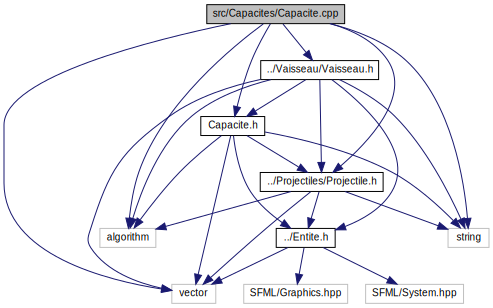
\includegraphics[width=350pt]{_capacite_8cpp__incl}
\end{center}
\end{figure}

\hypertarget{_capacite_8h}{}\section{Référence du fichier src/\+Capacite.h}
\label{_capacite_8h}\index{src/\+Capacite.\+h@{src/\+Capacite.\+h}}
\subsection*{Classes}
\begin{DoxyCompactItemize}
\item 
class \hyperlink{class_capacite}{Capacite}
\begin{DoxyCompactList}\small\item\em Classe virtuelle qui définit la structure générale d\textquotesingle{}une capacité \end{DoxyCompactList}\end{DoxyCompactItemize}

\hypertarget{_cap_aim_bot_8cpp}{}\section{Référence du fichier src/\+Capacites/\+Cap\+Aim\+Bot.cpp}
\label{_cap_aim_bot_8cpp}\index{src/\+Capacites/\+Cap\+Aim\+Bot.\+cpp@{src/\+Capacites/\+Cap\+Aim\+Bot.\+cpp}}
{\ttfamily \#include \char`\"{}Cap\+Aim\+Bot.\+h\char`\"{}}\newline
{\ttfamily \#include \char`\"{}Cap\+Missile.\+h\char`\"{}}\newline
Graphe des dépendances par inclusion de Cap\+Aim\+Bot.\+cpp\+:
% FIG 0

\hypertarget{_cap_aim_bot_8h}{}\section{Référence du fichier src/\+Capacites/\+Cap\+Aim\+Bot.h}
\label{_cap_aim_bot_8h}\index{src/\+Capacites/\+Cap\+Aim\+Bot.\+h@{src/\+Capacites/\+Cap\+Aim\+Bot.\+h}}
{\ttfamily \#include \char`\"{}Capacite.\+h\char`\"{}}\newline
Graphe des dépendances par inclusion de Cap\+Aim\+Bot.\+h\+:
% FIG 0
Ce graphe montre quels fichiers incluent directement ou indirectement ce fichier \+:
% FIG 1
\subsection*{Classes}
\begin{DoxyCompactItemize}
\item 
class \hyperlink{class_cap_aim_bot}{Cap\+Aim\+Bot}
\begin{DoxyCompactList}\small\item\em donne vis�e auto � un skill (missile) \end{DoxyCompactList}\end{DoxyCompactItemize}

\hypertarget{_cap_bismillah_beam_8cpp}{}\section{src/\+Capacites/\+Cap\+Bismillah\+Beam.cpp File Reference}
\label{_cap_bismillah_beam_8cpp}\index{src/\+Capacites/\+Cap\+Bismillah\+Beam.\+cpp@{src/\+Capacites/\+Cap\+Bismillah\+Beam.\+cpp}}
{\ttfamily \#include \char`\"{}Cap\+Bismillah\+Beam.\+h\char`\"{}}\newline
{\ttfamily \#include \char`\"{}../\+Projectiles/\+Proj\+Bismillah.\+h\char`\"{}}\newline

\hypertarget{_cap_bismillah_beam_8h}{}\section{Référence du fichier src/\+Capacites/\+Cap\+Bismillah\+Beam.h}
\label{_cap_bismillah_beam_8h}\index{src/\+Capacites/\+Cap\+Bismillah\+Beam.\+h@{src/\+Capacites/\+Cap\+Bismillah\+Beam.\+h}}
{\ttfamily \#include \char`\"{}Capacite.\+h\char`\"{}}\newline
Graphe des dépendances par inclusion de Cap\+Bismillah\+Beam.\+h\+:
% FIG 0
Ce graphe montre quels fichiers incluent directement ou indirectement ce fichier \+:
% FIG 1
\subsection*{Classes}
\begin{DoxyCompactItemize}
\item 
class \hyperlink{class_cap_bismillah}{Cap\+Bismillah}
\end{DoxyCompactItemize}

\hypertarget{_cap_boing_8cpp}{}\section{Référence du fichier src/\+Capacites/\+Cap\+Boing.cpp}
\label{_cap_boing_8cpp}\index{src/\+Capacites/\+Cap\+Boing.\+cpp@{src/\+Capacites/\+Cap\+Boing.\+cpp}}
{\ttfamily \#include \char`\"{}Cap\+Boing.\+h\char`\"{}}\newline
{\ttfamily \#include \char`\"{}Cap\+Dash.\+h\char`\"{}}\newline
Graphe des dépendances par inclusion de Cap\+Boing.\+cpp\+:
% FIG 0

\hypertarget{_cap_boing_8h}{}\section{src/\+Capacites/\+Cap\+Boing.h File Reference}
\label{_cap_boing_8h}\index{src/\+Capacites/\+Cap\+Boing.\+h@{src/\+Capacites/\+Cap\+Boing.\+h}}
{\ttfamily \#include \char`\"{}Capacite.\+h\char`\"{}}\newline
{\ttfamily \#include \char`\"{}../\+Projectiles/\+Projectile.\+h\char`\"{}}\newline
{\ttfamily \#include \char`\"{}../\+Projectiles/\+Proj\+Boing.\+h\char`\"{}}\newline
\subsection*{Classes}
\begin{DoxyCompactItemize}
\item 
class \mbox{\hyperlink{class_cap_boing}{Cap\+Boing}}
\begin{DoxyCompactList}\small\item\em Classe Capacité de test. \end{DoxyCompactList}\end{DoxyCompactItemize}

\hypertarget{_cap_bouclier_rond_8cpp}{}\section{Référence du fichier src/\+Capacites/\+Cap\+Bouclier\+Rond.cpp}
\label{_cap_bouclier_rond_8cpp}\index{src/\+Capacites/\+Cap\+Bouclier\+Rond.\+cpp@{src/\+Capacites/\+Cap\+Bouclier\+Rond.\+cpp}}
{\ttfamily \#include \char`\"{}Cap\+Bouclier\+Rond.\+h\char`\"{}}\newline
Graphe des dépendances par inclusion de Cap\+Bouclier\+Rond.\+cpp\+:
% FIG 0

\hypertarget{_cap_bouclier_rond_8h}{}\section{Référence du fichier src/\+Capacites/\+Cap\+Bouclier\+Rond.h}
\label{_cap_bouclier_rond_8h}\index{src/\+Capacites/\+Cap\+Bouclier\+Rond.\+h@{src/\+Capacites/\+Cap\+Bouclier\+Rond.\+h}}
{\ttfamily \#include \char`\"{}Capacite.\+h\char`\"{}}\newline
{\ttfamily \#include \char`\"{}../\+Projectiles/\+Projectile.\+h\char`\"{}}\newline
{\ttfamily \#include \char`\"{}../\+Projectiles/\+Proj\+Bouclier\+Rond.\+h\char`\"{}}\newline
Graphe des dépendances par inclusion de Cap\+Bouclier\+Rond.\+h\+:
% FIG 0
Ce graphe montre quels fichiers incluent directement ou indirectement ce fichier \+:
% FIG 1
\subsection*{Classes}
\begin{DoxyCompactItemize}
\item 
class \hyperlink{class_cap_bouclier_rond}{Cap\+Bouclier\+Rond}
\begin{DoxyCompactList}\small\item\em bouclier circulaire avec x PB \end{DoxyCompactList}\end{DoxyCompactItemize}

\hypertarget{_cap_dash_8cpp}{}\section{Référence du fichier src/\+Capacites/\+Cap\+Dash.cpp}
\label{_cap_dash_8cpp}\index{src/\+Capacites/\+Cap\+Dash.\+cpp@{src/\+Capacites/\+Cap\+Dash.\+cpp}}
{\ttfamily \#include \char`\"{}Cap\+Dash.\+h\char`\"{}}\newline
{\ttfamily \#include \char`\"{}../\+Interface/\+Input.\+h\char`\"{}}\newline
Graphe des dépendances par inclusion de Cap\+Dash.\+cpp\+:
% FIG 0

\hypertarget{_cap_dash_8h}{}\section{src/\+Capacites/\+Cap\+Dash.h File Reference}
\label{_cap_dash_8h}\index{src/\+Capacites/\+Cap\+Dash.\+h@{src/\+Capacites/\+Cap\+Dash.\+h}}
{\ttfamily \#include \char`\"{}Capacite.\+h\char`\"{}}\newline
{\ttfamily \#include \char`\"{}../\+Entite.\+h\char`\"{}}\newline
{\ttfamily \#include \char`\"{}../\+Projectiles/\+Proj\+Boing.\+h\char`\"{}}\newline
\subsection*{Classes}
\begin{DoxyCompactItemize}
\item 
class \mbox{\hyperlink{class_cap_dash}{Cap\+Dash}}
\begin{DoxyCompactList}\small\item\em Classe Capacité permettant de dash. \end{DoxyCompactList}\end{DoxyCompactItemize}

\hypertarget{_cap_missile_8cpp}{}\section{Référence du fichier src/\+Capacites/\+Cap\+Missile.cpp}
\label{_cap_missile_8cpp}\index{src/\+Capacites/\+Cap\+Missile.\+cpp@{src/\+Capacites/\+Cap\+Missile.\+cpp}}
{\ttfamily \#include \char`\"{}Cap\+Missile.\+h\char`\"{}}\newline
Graphe des dépendances par inclusion de Cap\+Missile.\+cpp\+:\nopagebreak
\begin{figure}[H]
\begin{center}
\leavevmode
\includegraphics[width=350pt]{_cap_missile_8cpp__incl}
\end{center}
\end{figure}

\hypertarget{_cap_missile_8h}{}\section{Référence du fichier src/\+Capacites/\+Cap\+Missile.h}
\label{_cap_missile_8h}\index{src/\+Capacites/\+Cap\+Missile.\+h@{src/\+Capacites/\+Cap\+Missile.\+h}}
{\ttfamily \#include \char`\"{}Capacite.\+h\char`\"{}}\newline
{\ttfamily \#include \char`\"{}../\+Projectiles/\+Proj\+Missile.\+h\char`\"{}}\newline
Graphe des dépendances par inclusion de Cap\+Missile.\+h\+:\nopagebreak
\begin{figure}[H]
\begin{center}
\leavevmode
\includegraphics[width=350pt]{_cap_missile_8h__incl}
\end{center}
\end{figure}
Ce graphe montre quels fichiers incluent directement ou indirectement ce fichier \+:\nopagebreak
\begin{figure}[H]
\begin{center}
\leavevmode
\includegraphics[width=350pt]{_cap_missile_8h__dep__incl}
\end{center}
\end{figure}
\subsection*{Classes}
\begin{DoxyCompactItemize}
\item 
class \hyperlink{class_cap_missile}{Cap\+Missile}
\begin{DoxyCompactList}\small\item\em Classe Capacité de base. \end{DoxyCompactList}\end{DoxyCompactItemize}

\hypertarget{_cap_piou_8cpp}{}\section{Référence du fichier src/\+Capacites/\+Cap\+Piou.cpp}
\label{_cap_piou_8cpp}\index{src/\+Capacites/\+Cap\+Piou.\+cpp@{src/\+Capacites/\+Cap\+Piou.\+cpp}}
{\ttfamily \#include \char`\"{}Cap\+Piou.\+h\char`\"{}}\newline
Graphe des dépendances par inclusion de Cap\+Piou.\+cpp\+:
\nopagebreak
\begin{figure}[H]
\begin{center}
\leavevmode
\includegraphics[width=350pt]{_cap_piou_8cpp__incl}
\end{center}
\end{figure}

\hypertarget{_cap_piou_8h}{}\section{Référence du fichier src/\+Capacites/\+Cap\+Piou.h}
\label{_cap_piou_8h}\index{src/\+Capacites/\+Cap\+Piou.\+h@{src/\+Capacites/\+Cap\+Piou.\+h}}
{\ttfamily \#include \char`\"{}Capacite.\+h\char`\"{}}\newline
{\ttfamily \#include \char`\"{}../\+Projectiles/\+Projectile.\+h\char`\"{}}\newline
{\ttfamily \#include \char`\"{}../\+Projectiles/\+Proj\+Piou.\+h\char`\"{}}\newline
Graphe des dépendances par inclusion de Cap\+Piou.\+h\+:
% FIG 0
Ce graphe montre quels fichiers incluent directement ou indirectement ce fichier \+:
% FIG 1
\subsection*{Classes}
\begin{DoxyCompactItemize}
\item 
class \hyperlink{class_cap_piou}{Cap\+Piou}
\begin{DoxyCompactList}\small\item\em Classe Capacité de base. \end{DoxyCompactList}\end{DoxyCompactItemize}

\hypertarget{constantes_8h}{}\section{src/constantes.h File Reference}
\label{constantes_8h}\index{src/constantes.\+h@{src/constantes.\+h}}
{\ttfamily \#include $<$cstddef$>$}\newline
\subsection*{Macros}
\begin{DoxyCompactItemize}
\item 
\#define \mbox{\hyperlink{constantes_8h_aa55807c5b694c7cefe344e8b78e5aadb}{chemin\+\_\+rc}}~\char`\"{}../../rc/\char`\"{}
\item 
\#define \mbox{\hyperlink{constantes_8h_a598a3330b3c21701223ee0ca14316eca}{PI}}~acos(-\/1.\+0)
\item 
\#define \mbox{\hyperlink{constantes_8h_a1c6d5de492ac61ad29aec7aa9a436bbf}{V\+E\+R\+S\+I\+ON}}~\char`\"{}Debug.\char`\"{}
\item 
\#define \mbox{\hyperlink{constantes_8h_ad9816adb4ece0656cd3d58f627b107db}{B\+R\+A\+N\+C\+HE}}~\char`\"{}Nettoyage de printemps\char`\"{}
\end{DoxyCompactItemize}
\subsection*{Enumerations}
\begin{DoxyCompactItemize}
\item 
enum \mbox{\hyperlink{constantes_8h_a250372292659bed7ae290d8621f88ccf}{Actions}} \{ \newline
\mbox{\hyperlink{constantes_8h_a250372292659bed7ae290d8621f88ccfa56b36d0d0bb01b339cf1041adc08e262}{P\+A\+U\+SE}}, 
\mbox{\hyperlink{constantes_8h_a250372292659bed7ae290d8621f88ccfa44466ad40cb0a09371d2b828b36c48e7}{T\+I\+R1}}, 
\mbox{\hyperlink{constantes_8h_a250372292659bed7ae290d8621f88ccfac9439845b5972a9dc101085343ac065c}{T\+I\+R2}}, 
\mbox{\hyperlink{constantes_8h_a250372292659bed7ae290d8621f88ccfa157fc740ff7ff2c0247ac5961f66009c}{C\+O\+M\+P1}}, 
\newline
\mbox{\hyperlink{constantes_8h_a250372292659bed7ae290d8621f88ccfa56bb8c406fa7684dc34ffe1a6d389565}{C\+O\+M\+P2}}, 
\mbox{\hyperlink{constantes_8h_a250372292659bed7ae290d8621f88ccfaccc8850f02d2db3d2e39bec5295edc46}{C\+O\+M\+P3}}, 
\mbox{\hyperlink{constantes_8h_a250372292659bed7ae290d8621f88ccfa26cfa63737372a3312d10aebb767d603}{U\+L\+TI}}
 \}
\item 
enum \mbox{\hyperlink{constantes_8h_a08fa5554288d5031a8f3bb83cc04ee83}{Equipe}} \{ \mbox{\hyperlink{constantes_8h_a08fa5554288d5031a8f3bb83cc04ee83ad4d15427af4b5b0f54dbed84f89cade7}{J\+O\+U\+E\+UR}}, 
\mbox{\hyperlink{constantes_8h_a08fa5554288d5031a8f3bb83cc04ee83a6c21d8eea108820375064b6acafce3f9}{E\+N\+N\+E\+MI}}, 
\mbox{\hyperlink{constantes_8h_a08fa5554288d5031a8f3bb83cc04ee83a31ad00d2974deb1103ea000de3bff57d}{N\+E\+U\+T\+RE}}, 
\mbox{\hyperlink{constantes_8h_a08fa5554288d5031a8f3bb83cc04ee83a720a6a0fa0be9398650409a7befa7293}{A\+L\+L\+IE}}
 \}
\item 
enum \mbox{\hyperlink{constantes_8h_a33e4f15dde10f34860a6b35be343ae56}{ecran\+\_\+t}} \{ \mbox{\hyperlink{constantes_8h_a33e4f15dde10f34860a6b35be343ae56ad4686f4f969d0e851d9170c09a89a837}{V\+I\+DE}} = -\/1, 
\mbox{\hyperlink{constantes_8h_a33e4f15dde10f34860a6b35be343ae56a96251739b593a8e10380d58a30e93fd8}{A\+C\+C\+U\+E\+IL}} = 0, 
\mbox{\hyperlink{constantes_8h_a33e4f15dde10f34860a6b35be343ae56ad84154820fb7cc5480aa99b8e888ef2e}{M\+E\+N\+U\+\_\+\+P\+R\+I\+N\+C\+I\+P\+AL}}, 
\mbox{\hyperlink{constantes_8h_a33e4f15dde10f34860a6b35be343ae56adb639f85bf0a305a48b5874ea027a831}{P\+A\+R\+T\+IE}}
 \}
\end{DoxyCompactItemize}
\subsection*{Variables}
\begin{DoxyCompactItemize}
\item 
constexpr float \mbox{\hyperlink{constantes_8h_a8958557e953d458537dedcf460f477c1}{E\+C\+R\+A\+N\+\_\+L}} = 1024
\item 
constexpr float \mbox{\hyperlink{constantes_8h_a899c06d4fdb39f4fa51fc7158e2be2d1}{E\+C\+R\+A\+N\+\_\+H}} = 768
\begin{DoxyCompactList}\small\item\em Largueur de la fenetre. \end{DoxyCompactList}\item 
constexpr float \mbox{\hyperlink{constantes_8h_ac48605b788819fe8dcad2622d7f1f00c}{O\+V\+E\+R\+L\+A\+Y\+\_\+\+B\+A\+R\+R\+E\+\_\+L}} = 500
\begin{DoxyCompactList}\small\item\em Hauteur de la fenetre. \end{DoxyCompactList}\item 
constexpr float \mbox{\hyperlink{constantes_8h_aec53a7a575e951f65fca395d860ff1c6}{O\+V\+E\+R\+L\+A\+Y\+\_\+\+B\+A\+R\+R\+E\+\_\+H}} = 16
\begin{DoxyCompactList}\small\item\em Largueur des barres de l\textquotesingle{}overlay. \end{DoxyCompactList}\item 
constexpr size\+\_\+t \mbox{\hyperlink{constantes_8h_abd929aee9ec2e5d880b87ac867ad49e1}{N\+B\+\_\+\+A\+C\+T\+I\+ON}} = 7
\begin{DoxyCompactList}\small\item\em Hauteur des barres de l\textquotesingle{}overlay. \end{DoxyCompactList}\item 
constexpr size\+\_\+t \mbox{\hyperlink{constantes_8h_ad4a41a3da7bd10b3350047db17a78ee6}{T\+E\+M\+P\+S\+\_\+\+I\+N\+V\+I\+N\+C\+I\+B\+I\+L\+I\+TE}} = 2000
\begin{DoxyCompactList}\small\item\em Nombre d\textquotesingle{}actions. \end{DoxyCompactList}\item 
constexpr bool \mbox{\hyperlink{constantes_8h_a7507bfee1d3f050ad869013d74424e9e}{D\+E\+B\+UG}} = true
\begin{DoxyCompactList}\small\item\em Nombres de millisecondes d\textquotesingle{}invincibilité par défaut. \end{DoxyCompactList}\end{DoxyCompactItemize}


\subsection{Macro Definition Documentation}
\mbox{\Hypertarget{constantes_8h_ad9816adb4ece0656cd3d58f627b107db}\label{constantes_8h_ad9816adb4ece0656cd3d58f627b107db}} 
\index{constantes.\+h@{constantes.\+h}!B\+R\+A\+N\+C\+HE@{B\+R\+A\+N\+C\+HE}}
\index{B\+R\+A\+N\+C\+HE@{B\+R\+A\+N\+C\+HE}!constantes.\+h@{constantes.\+h}}
\subsubsection{\texorpdfstring{B\+R\+A\+N\+C\+HE}{BRANCHE}}
{\footnotesize\ttfamily \#define B\+R\+A\+N\+C\+HE~\char`\"{}Nettoyage de printemps\char`\"{}}

\mbox{\Hypertarget{constantes_8h_aa55807c5b694c7cefe344e8b78e5aadb}\label{constantes_8h_aa55807c5b694c7cefe344e8b78e5aadb}} 
\index{constantes.\+h@{constantes.\+h}!chemin\+\_\+rc@{chemin\+\_\+rc}}
\index{chemin\+\_\+rc@{chemin\+\_\+rc}!constantes.\+h@{constantes.\+h}}
\subsubsection{\texorpdfstring{chemin\+\_\+rc}{chemin\_rc}}
{\footnotesize\ttfamily \#define chemin\+\_\+rc~\char`\"{}../../rc/\char`\"{}}

\mbox{\Hypertarget{constantes_8h_a598a3330b3c21701223ee0ca14316eca}\label{constantes_8h_a598a3330b3c21701223ee0ca14316eca}} 
\index{constantes.\+h@{constantes.\+h}!PI@{PI}}
\index{PI@{PI}!constantes.\+h@{constantes.\+h}}
\subsubsection{\texorpdfstring{PI}{PI}}
{\footnotesize\ttfamily \#define PI~acos(-\/1.\+0)}

\mbox{\Hypertarget{constantes_8h_a1c6d5de492ac61ad29aec7aa9a436bbf}\label{constantes_8h_a1c6d5de492ac61ad29aec7aa9a436bbf}} 
\index{constantes.\+h@{constantes.\+h}!V\+E\+R\+S\+I\+ON@{V\+E\+R\+S\+I\+ON}}
\index{V\+E\+R\+S\+I\+ON@{V\+E\+R\+S\+I\+ON}!constantes.\+h@{constantes.\+h}}
\subsubsection{\texorpdfstring{V\+E\+R\+S\+I\+ON}{VERSION}}
{\footnotesize\ttfamily \#define V\+E\+R\+S\+I\+ON~\char`\"{}Debug.\char`\"{}}



\subsection{Enumeration Type Documentation}
\mbox{\Hypertarget{constantes_8h_a250372292659bed7ae290d8621f88ccf}\label{constantes_8h_a250372292659bed7ae290d8621f88ccf}} 
\index{constantes.\+h@{constantes.\+h}!Actions@{Actions}}
\index{Actions@{Actions}!constantes.\+h@{constantes.\+h}}
\subsubsection{\texorpdfstring{Actions}{Actions}}
{\footnotesize\ttfamily enum \mbox{\hyperlink{constantes_8h_a250372292659bed7ae290d8621f88ccf}{Actions}}}

\begin{DoxyEnumFields}{Enumerator}
\raisebox{\heightof{T}}[0pt][0pt]{\index{P\+A\+U\+SE@{P\+A\+U\+SE}!constantes.\+h@{constantes.\+h}}\index{constantes.\+h@{constantes.\+h}!P\+A\+U\+SE@{P\+A\+U\+SE}}}\mbox{\Hypertarget{constantes_8h_a250372292659bed7ae290d8621f88ccfa56b36d0d0bb01b339cf1041adc08e262}\label{constantes_8h_a250372292659bed7ae290d8621f88ccfa56b36d0d0bb01b339cf1041adc08e262}} 
P\+A\+U\+SE&\\
\hline

\raisebox{\heightof{T}}[0pt][0pt]{\index{T\+I\+R1@{T\+I\+R1}!constantes.\+h@{constantes.\+h}}\index{constantes.\+h@{constantes.\+h}!T\+I\+R1@{T\+I\+R1}}}\mbox{\Hypertarget{constantes_8h_a250372292659bed7ae290d8621f88ccfa44466ad40cb0a09371d2b828b36c48e7}\label{constantes_8h_a250372292659bed7ae290d8621f88ccfa44466ad40cb0a09371d2b828b36c48e7}} 
T\+I\+R1&\\
\hline

\raisebox{\heightof{T}}[0pt][0pt]{\index{T\+I\+R2@{T\+I\+R2}!constantes.\+h@{constantes.\+h}}\index{constantes.\+h@{constantes.\+h}!T\+I\+R2@{T\+I\+R2}}}\mbox{\Hypertarget{constantes_8h_a250372292659bed7ae290d8621f88ccfac9439845b5972a9dc101085343ac065c}\label{constantes_8h_a250372292659bed7ae290d8621f88ccfac9439845b5972a9dc101085343ac065c}} 
T\+I\+R2&\\
\hline

\raisebox{\heightof{T}}[0pt][0pt]{\index{C\+O\+M\+P1@{C\+O\+M\+P1}!constantes.\+h@{constantes.\+h}}\index{constantes.\+h@{constantes.\+h}!C\+O\+M\+P1@{C\+O\+M\+P1}}}\mbox{\Hypertarget{constantes_8h_a250372292659bed7ae290d8621f88ccfa157fc740ff7ff2c0247ac5961f66009c}\label{constantes_8h_a250372292659bed7ae290d8621f88ccfa157fc740ff7ff2c0247ac5961f66009c}} 
C\+O\+M\+P1&\\
\hline

\raisebox{\heightof{T}}[0pt][0pt]{\index{C\+O\+M\+P2@{C\+O\+M\+P2}!constantes.\+h@{constantes.\+h}}\index{constantes.\+h@{constantes.\+h}!C\+O\+M\+P2@{C\+O\+M\+P2}}}\mbox{\Hypertarget{constantes_8h_a250372292659bed7ae290d8621f88ccfa56bb8c406fa7684dc34ffe1a6d389565}\label{constantes_8h_a250372292659bed7ae290d8621f88ccfa56bb8c406fa7684dc34ffe1a6d389565}} 
C\+O\+M\+P2&\\
\hline

\raisebox{\heightof{T}}[0pt][0pt]{\index{C\+O\+M\+P3@{C\+O\+M\+P3}!constantes.\+h@{constantes.\+h}}\index{constantes.\+h@{constantes.\+h}!C\+O\+M\+P3@{C\+O\+M\+P3}}}\mbox{\Hypertarget{constantes_8h_a250372292659bed7ae290d8621f88ccfaccc8850f02d2db3d2e39bec5295edc46}\label{constantes_8h_a250372292659bed7ae290d8621f88ccfaccc8850f02d2db3d2e39bec5295edc46}} 
C\+O\+M\+P3&\\
\hline

\raisebox{\heightof{T}}[0pt][0pt]{\index{U\+L\+TI@{U\+L\+TI}!constantes.\+h@{constantes.\+h}}\index{constantes.\+h@{constantes.\+h}!U\+L\+TI@{U\+L\+TI}}}\mbox{\Hypertarget{constantes_8h_a250372292659bed7ae290d8621f88ccfa26cfa63737372a3312d10aebb767d603}\label{constantes_8h_a250372292659bed7ae290d8621f88ccfa26cfa63737372a3312d10aebb767d603}} 
U\+L\+TI&\\
\hline

\end{DoxyEnumFields}
\mbox{\Hypertarget{constantes_8h_a33e4f15dde10f34860a6b35be343ae56}\label{constantes_8h_a33e4f15dde10f34860a6b35be343ae56}} 
\index{constantes.\+h@{constantes.\+h}!ecran\+\_\+t@{ecran\+\_\+t}}
\index{ecran\+\_\+t@{ecran\+\_\+t}!constantes.\+h@{constantes.\+h}}
\subsubsection{\texorpdfstring{ecran\+\_\+t}{ecran\_t}}
{\footnotesize\ttfamily enum \mbox{\hyperlink{constantes_8h_a33e4f15dde10f34860a6b35be343ae56}{ecran\+\_\+t}}}

\begin{DoxyEnumFields}{Enumerator}
\raisebox{\heightof{T}}[0pt][0pt]{\index{V\+I\+DE@{V\+I\+DE}!constantes.\+h@{constantes.\+h}}\index{constantes.\+h@{constantes.\+h}!V\+I\+DE@{V\+I\+DE}}}\mbox{\Hypertarget{constantes_8h_a33e4f15dde10f34860a6b35be343ae56ad4686f4f969d0e851d9170c09a89a837}\label{constantes_8h_a33e4f15dde10f34860a6b35be343ae56ad4686f4f969d0e851d9170c09a89a837}} 
V\+I\+DE&\\
\hline

\raisebox{\heightof{T}}[0pt][0pt]{\index{A\+C\+C\+U\+E\+IL@{A\+C\+C\+U\+E\+IL}!constantes.\+h@{constantes.\+h}}\index{constantes.\+h@{constantes.\+h}!A\+C\+C\+U\+E\+IL@{A\+C\+C\+U\+E\+IL}}}\mbox{\Hypertarget{constantes_8h_a33e4f15dde10f34860a6b35be343ae56a96251739b593a8e10380d58a30e93fd8}\label{constantes_8h_a33e4f15dde10f34860a6b35be343ae56a96251739b593a8e10380d58a30e93fd8}} 
A\+C\+C\+U\+E\+IL&\\
\hline

\raisebox{\heightof{T}}[0pt][0pt]{\index{M\+E\+N\+U\+\_\+\+P\+R\+I\+N\+C\+I\+P\+AL@{M\+E\+N\+U\+\_\+\+P\+R\+I\+N\+C\+I\+P\+AL}!constantes.\+h@{constantes.\+h}}\index{constantes.\+h@{constantes.\+h}!M\+E\+N\+U\+\_\+\+P\+R\+I\+N\+C\+I\+P\+AL@{M\+E\+N\+U\+\_\+\+P\+R\+I\+N\+C\+I\+P\+AL}}}\mbox{\Hypertarget{constantes_8h_a33e4f15dde10f34860a6b35be343ae56ad84154820fb7cc5480aa99b8e888ef2e}\label{constantes_8h_a33e4f15dde10f34860a6b35be343ae56ad84154820fb7cc5480aa99b8e888ef2e}} 
M\+E\+N\+U\+\_\+\+P\+R\+I\+N\+C\+I\+P\+AL&\\
\hline

\raisebox{\heightof{T}}[0pt][0pt]{\index{P\+A\+R\+T\+IE@{P\+A\+R\+T\+IE}!constantes.\+h@{constantes.\+h}}\index{constantes.\+h@{constantes.\+h}!P\+A\+R\+T\+IE@{P\+A\+R\+T\+IE}}}\mbox{\Hypertarget{constantes_8h_a33e4f15dde10f34860a6b35be343ae56adb639f85bf0a305a48b5874ea027a831}\label{constantes_8h_a33e4f15dde10f34860a6b35be343ae56adb639f85bf0a305a48b5874ea027a831}} 
P\+A\+R\+T\+IE&\\
\hline

\end{DoxyEnumFields}
\mbox{\Hypertarget{constantes_8h_a08fa5554288d5031a8f3bb83cc04ee83}\label{constantes_8h_a08fa5554288d5031a8f3bb83cc04ee83}} 
\index{constantes.\+h@{constantes.\+h}!Equipe@{Equipe}}
\index{Equipe@{Equipe}!constantes.\+h@{constantes.\+h}}
\subsubsection{\texorpdfstring{Equipe}{Equipe}}
{\footnotesize\ttfamily enum \mbox{\hyperlink{constantes_8h_a08fa5554288d5031a8f3bb83cc04ee83}{Equipe}}}

\begin{DoxyEnumFields}{Enumerator}
\raisebox{\heightof{T}}[0pt][0pt]{\index{J\+O\+U\+E\+UR@{J\+O\+U\+E\+UR}!constantes.\+h@{constantes.\+h}}\index{constantes.\+h@{constantes.\+h}!J\+O\+U\+E\+UR@{J\+O\+U\+E\+UR}}}\mbox{\Hypertarget{constantes_8h_a08fa5554288d5031a8f3bb83cc04ee83ad4d15427af4b5b0f54dbed84f89cade7}\label{constantes_8h_a08fa5554288d5031a8f3bb83cc04ee83ad4d15427af4b5b0f54dbed84f89cade7}} 
J\+O\+U\+E\+UR&\\
\hline

\raisebox{\heightof{T}}[0pt][0pt]{\index{E\+N\+N\+E\+MI@{E\+N\+N\+E\+MI}!constantes.\+h@{constantes.\+h}}\index{constantes.\+h@{constantes.\+h}!E\+N\+N\+E\+MI@{E\+N\+N\+E\+MI}}}\mbox{\Hypertarget{constantes_8h_a08fa5554288d5031a8f3bb83cc04ee83a6c21d8eea108820375064b6acafce3f9}\label{constantes_8h_a08fa5554288d5031a8f3bb83cc04ee83a6c21d8eea108820375064b6acafce3f9}} 
E\+N\+N\+E\+MI&\\
\hline

\raisebox{\heightof{T}}[0pt][0pt]{\index{N\+E\+U\+T\+RE@{N\+E\+U\+T\+RE}!constantes.\+h@{constantes.\+h}}\index{constantes.\+h@{constantes.\+h}!N\+E\+U\+T\+RE@{N\+E\+U\+T\+RE}}}\mbox{\Hypertarget{constantes_8h_a08fa5554288d5031a8f3bb83cc04ee83a31ad00d2974deb1103ea000de3bff57d}\label{constantes_8h_a08fa5554288d5031a8f3bb83cc04ee83a31ad00d2974deb1103ea000de3bff57d}} 
N\+E\+U\+T\+RE&\\
\hline

\raisebox{\heightof{T}}[0pt][0pt]{\index{A\+L\+L\+IE@{A\+L\+L\+IE}!constantes.\+h@{constantes.\+h}}\index{constantes.\+h@{constantes.\+h}!A\+L\+L\+IE@{A\+L\+L\+IE}}}\mbox{\Hypertarget{constantes_8h_a08fa5554288d5031a8f3bb83cc04ee83a720a6a0fa0be9398650409a7befa7293}\label{constantes_8h_a08fa5554288d5031a8f3bb83cc04ee83a720a6a0fa0be9398650409a7befa7293}} 
A\+L\+L\+IE&\\
\hline

\end{DoxyEnumFields}


\subsection{Variable Documentation}
\mbox{\Hypertarget{constantes_8h_a7507bfee1d3f050ad869013d74424e9e}\label{constantes_8h_a7507bfee1d3f050ad869013d74424e9e}} 
\index{constantes.\+h@{constantes.\+h}!D\+E\+B\+UG@{D\+E\+B\+UG}}
\index{D\+E\+B\+UG@{D\+E\+B\+UG}!constantes.\+h@{constantes.\+h}}
\subsubsection{\texorpdfstring{D\+E\+B\+UG}{DEBUG}}
{\footnotesize\ttfamily constexpr bool D\+E\+B\+UG = true}



Nombres de millisecondes d\textquotesingle{}invincibilité par défaut. 

\mbox{\Hypertarget{constantes_8h_a899c06d4fdb39f4fa51fc7158e2be2d1}\label{constantes_8h_a899c06d4fdb39f4fa51fc7158e2be2d1}} 
\index{constantes.\+h@{constantes.\+h}!E\+C\+R\+A\+N\+\_\+H@{E\+C\+R\+A\+N\+\_\+H}}
\index{E\+C\+R\+A\+N\+\_\+H@{E\+C\+R\+A\+N\+\_\+H}!constantes.\+h@{constantes.\+h}}
\subsubsection{\texorpdfstring{E\+C\+R\+A\+N\+\_\+H}{ECRAN\_H}}
{\footnotesize\ttfamily constexpr float E\+C\+R\+A\+N\+\_\+H = 768}



Largueur de la fenetre. 

\mbox{\Hypertarget{constantes_8h_a8958557e953d458537dedcf460f477c1}\label{constantes_8h_a8958557e953d458537dedcf460f477c1}} 
\index{constantes.\+h@{constantes.\+h}!E\+C\+R\+A\+N\+\_\+L@{E\+C\+R\+A\+N\+\_\+L}}
\index{E\+C\+R\+A\+N\+\_\+L@{E\+C\+R\+A\+N\+\_\+L}!constantes.\+h@{constantes.\+h}}
\subsubsection{\texorpdfstring{E\+C\+R\+A\+N\+\_\+L}{ECRAN\_L}}
{\footnotesize\ttfamily constexpr float E\+C\+R\+A\+N\+\_\+L = 1024}

\mbox{\Hypertarget{constantes_8h_abd929aee9ec2e5d880b87ac867ad49e1}\label{constantes_8h_abd929aee9ec2e5d880b87ac867ad49e1}} 
\index{constantes.\+h@{constantes.\+h}!N\+B\+\_\+\+A\+C\+T\+I\+ON@{N\+B\+\_\+\+A\+C\+T\+I\+ON}}
\index{N\+B\+\_\+\+A\+C\+T\+I\+ON@{N\+B\+\_\+\+A\+C\+T\+I\+ON}!constantes.\+h@{constantes.\+h}}
\subsubsection{\texorpdfstring{N\+B\+\_\+\+A\+C\+T\+I\+ON}{NB\_ACTION}}
{\footnotesize\ttfamily constexpr size\+\_\+t N\+B\+\_\+\+A\+C\+T\+I\+ON = 7}



Hauteur des barres de l\textquotesingle{}overlay. 

\mbox{\Hypertarget{constantes_8h_aec53a7a575e951f65fca395d860ff1c6}\label{constantes_8h_aec53a7a575e951f65fca395d860ff1c6}} 
\index{constantes.\+h@{constantes.\+h}!O\+V\+E\+R\+L\+A\+Y\+\_\+\+B\+A\+R\+R\+E\+\_\+H@{O\+V\+E\+R\+L\+A\+Y\+\_\+\+B\+A\+R\+R\+E\+\_\+H}}
\index{O\+V\+E\+R\+L\+A\+Y\+\_\+\+B\+A\+R\+R\+E\+\_\+H@{O\+V\+E\+R\+L\+A\+Y\+\_\+\+B\+A\+R\+R\+E\+\_\+H}!constantes.\+h@{constantes.\+h}}
\subsubsection{\texorpdfstring{O\+V\+E\+R\+L\+A\+Y\+\_\+\+B\+A\+R\+R\+E\+\_\+H}{OVERLAY\_BARRE\_H}}
{\footnotesize\ttfamily constexpr float O\+V\+E\+R\+L\+A\+Y\+\_\+\+B\+A\+R\+R\+E\+\_\+H = 16}



Largueur des barres de l\textquotesingle{}overlay. 

\mbox{\Hypertarget{constantes_8h_ac48605b788819fe8dcad2622d7f1f00c}\label{constantes_8h_ac48605b788819fe8dcad2622d7f1f00c}} 
\index{constantes.\+h@{constantes.\+h}!O\+V\+E\+R\+L\+A\+Y\+\_\+\+B\+A\+R\+R\+E\+\_\+L@{O\+V\+E\+R\+L\+A\+Y\+\_\+\+B\+A\+R\+R\+E\+\_\+L}}
\index{O\+V\+E\+R\+L\+A\+Y\+\_\+\+B\+A\+R\+R\+E\+\_\+L@{O\+V\+E\+R\+L\+A\+Y\+\_\+\+B\+A\+R\+R\+E\+\_\+L}!constantes.\+h@{constantes.\+h}}
\subsubsection{\texorpdfstring{O\+V\+E\+R\+L\+A\+Y\+\_\+\+B\+A\+R\+R\+E\+\_\+L}{OVERLAY\_BARRE\_L}}
{\footnotesize\ttfamily constexpr float O\+V\+E\+R\+L\+A\+Y\+\_\+\+B\+A\+R\+R\+E\+\_\+L = 500}



Hauteur de la fenetre. 

\mbox{\Hypertarget{constantes_8h_ad4a41a3da7bd10b3350047db17a78ee6}\label{constantes_8h_ad4a41a3da7bd10b3350047db17a78ee6}} 
\index{constantes.\+h@{constantes.\+h}!T\+E\+M\+P\+S\+\_\+\+I\+N\+V\+I\+N\+C\+I\+B\+I\+L\+I\+TE@{T\+E\+M\+P\+S\+\_\+\+I\+N\+V\+I\+N\+C\+I\+B\+I\+L\+I\+TE}}
\index{T\+E\+M\+P\+S\+\_\+\+I\+N\+V\+I\+N\+C\+I\+B\+I\+L\+I\+TE@{T\+E\+M\+P\+S\+\_\+\+I\+N\+V\+I\+N\+C\+I\+B\+I\+L\+I\+TE}!constantes.\+h@{constantes.\+h}}
\subsubsection{\texorpdfstring{T\+E\+M\+P\+S\+\_\+\+I\+N\+V\+I\+N\+C\+I\+B\+I\+L\+I\+TE}{TEMPS\_INVINCIBILITE}}
{\footnotesize\ttfamily constexpr size\+\_\+t T\+E\+M\+P\+S\+\_\+\+I\+N\+V\+I\+N\+C\+I\+B\+I\+L\+I\+TE = 2000}



Nombre d\textquotesingle{}actions. 


\hypertarget{def__type_8h}{}\section{src/def\+\_\+type.h File Reference}
\label{def__type_8h}\index{src/def\+\_\+type.\+h@{src/def\+\_\+type.\+h}}
{\ttfamily \#include $<$memory$>$}\newline
{\ttfamily \#include $<$vector$>$}\newline
\subsection*{Typedefs}
\begin{DoxyCompactItemize}
\item 
using \mbox{\hyperlink{def__type_8h_a03925a047830157ad843b4224e7f63ba}{vaisseau\+\_\+ptr}} = std\+::shared\+\_\+ptr$<$ \mbox{\hyperlink{class_vaisseau}{Vaisseau}} $>$
\item 
using \mbox{\hyperlink{def__type_8h_ad123ed7c93f42c8dd68e4af28b16b639}{vaisseau\+\_\+container}} = std\+::vector$<$ \mbox{\hyperlink{def__type_8h_a03925a047830157ad843b4224e7f63ba}{vaisseau\+\_\+ptr}} $>$
\item 
using \mbox{\hyperlink{def__type_8h_a0ed393286e5026881321a018ea6ab328}{proj\+\_\+ptr}} = std\+::shared\+\_\+ptr$<$ \mbox{\hyperlink{class_projectile}{Projectile}} $>$
\item 
using \mbox{\hyperlink{def__type_8h_a87980cd8ee9533e561a73e8bbc728188}{proj\+\_\+container}} = std\+::vector$<$ \mbox{\hyperlink{def__type_8h_a0ed393286e5026881321a018ea6ab328}{proj\+\_\+ptr}} $>$
\item 
using \mbox{\hyperlink{def__type_8h_a52e6a5cf43a2860d551b1af43488f954}{entite\+\_\+ptr}} = std\+::shared\+\_\+ptr$<$ \mbox{\hyperlink{class_entite}{Entite}} $>$
\end{DoxyCompactItemize}


\subsection{Typedef Documentation}
\mbox{\Hypertarget{def__type_8h_a52e6a5cf43a2860d551b1af43488f954}\label{def__type_8h_a52e6a5cf43a2860d551b1af43488f954}} 
\index{def\+\_\+type.\+h@{def\+\_\+type.\+h}!entite\+\_\+ptr@{entite\+\_\+ptr}}
\index{entite\+\_\+ptr@{entite\+\_\+ptr}!def\+\_\+type.\+h@{def\+\_\+type.\+h}}
\subsubsection{\texorpdfstring{entite\+\_\+ptr}{entite\_ptr}}
{\footnotesize\ttfamily using \mbox{\hyperlink{def__type_8h_a52e6a5cf43a2860d551b1af43488f954}{entite\+\_\+ptr}} =  std\+::shared\+\_\+ptr$<$\mbox{\hyperlink{class_entite}{Entite}}$>$}

\mbox{\Hypertarget{def__type_8h_a87980cd8ee9533e561a73e8bbc728188}\label{def__type_8h_a87980cd8ee9533e561a73e8bbc728188}} 
\index{def\+\_\+type.\+h@{def\+\_\+type.\+h}!proj\+\_\+container@{proj\+\_\+container}}
\index{proj\+\_\+container@{proj\+\_\+container}!def\+\_\+type.\+h@{def\+\_\+type.\+h}}
\subsubsection{\texorpdfstring{proj\+\_\+container}{proj\_container}}
{\footnotesize\ttfamily using \mbox{\hyperlink{def__type_8h_a87980cd8ee9533e561a73e8bbc728188}{proj\+\_\+container}} =  std\+::vector$<$\mbox{\hyperlink{def__type_8h_a0ed393286e5026881321a018ea6ab328}{proj\+\_\+ptr}}$>$}

\mbox{\Hypertarget{def__type_8h_a0ed393286e5026881321a018ea6ab328}\label{def__type_8h_a0ed393286e5026881321a018ea6ab328}} 
\index{def\+\_\+type.\+h@{def\+\_\+type.\+h}!proj\+\_\+ptr@{proj\+\_\+ptr}}
\index{proj\+\_\+ptr@{proj\+\_\+ptr}!def\+\_\+type.\+h@{def\+\_\+type.\+h}}
\subsubsection{\texorpdfstring{proj\+\_\+ptr}{proj\_ptr}}
{\footnotesize\ttfamily using \mbox{\hyperlink{def__type_8h_a0ed393286e5026881321a018ea6ab328}{proj\+\_\+ptr}} =  std\+::shared\+\_\+ptr$<$\mbox{\hyperlink{class_projectile}{Projectile}}$>$}

\mbox{\Hypertarget{def__type_8h_ad123ed7c93f42c8dd68e4af28b16b639}\label{def__type_8h_ad123ed7c93f42c8dd68e4af28b16b639}} 
\index{def\+\_\+type.\+h@{def\+\_\+type.\+h}!vaisseau\+\_\+container@{vaisseau\+\_\+container}}
\index{vaisseau\+\_\+container@{vaisseau\+\_\+container}!def\+\_\+type.\+h@{def\+\_\+type.\+h}}
\subsubsection{\texorpdfstring{vaisseau\+\_\+container}{vaisseau\_container}}
{\footnotesize\ttfamily using \mbox{\hyperlink{def__type_8h_ad123ed7c93f42c8dd68e4af28b16b639}{vaisseau\+\_\+container}} =  std\+::vector$<$\mbox{\hyperlink{def__type_8h_a03925a047830157ad843b4224e7f63ba}{vaisseau\+\_\+ptr}}$>$}

\mbox{\Hypertarget{def__type_8h_a03925a047830157ad843b4224e7f63ba}\label{def__type_8h_a03925a047830157ad843b4224e7f63ba}} 
\index{def\+\_\+type.\+h@{def\+\_\+type.\+h}!vaisseau\+\_\+ptr@{vaisseau\+\_\+ptr}}
\index{vaisseau\+\_\+ptr@{vaisseau\+\_\+ptr}!def\+\_\+type.\+h@{def\+\_\+type.\+h}}
\subsubsection{\texorpdfstring{vaisseau\+\_\+ptr}{vaisseau\_ptr}}
{\footnotesize\ttfamily using \mbox{\hyperlink{def__type_8h_a03925a047830157ad843b4224e7f63ba}{vaisseau\+\_\+ptr}} =  std\+::shared\+\_\+ptr$<$\mbox{\hyperlink{class_vaisseau}{Vaisseau}}$>$}


\hypertarget{_entite_8cpp}{}\section{src/\+Entite.cpp File Reference}
\label{_entite_8cpp}\index{src/\+Entite.\+cpp@{src/\+Entite.\+cpp}}
{\ttfamily \#include \char`\"{}Entite.\+h\char`\"{}}\newline
{\ttfamily \#include \char`\"{}Utilitaires/\+Collision.\+h\char`\"{}}\newline
{\ttfamily \#include \char`\"{}constantes.\+h\char`\"{}}\newline
{\ttfamily \#include $<$cmath$>$}\newline
\subsection*{Functions}
\begin{DoxyCompactItemize}
\item 
bool \mbox{\hyperlink{_entite_8cpp_ac85cf277aaeb8a314734c1fa5f35e3be}{collision}} (const \mbox{\hyperlink{class_entite}{Entite}} \&e1, const \mbox{\hyperlink{class_entite}{Entite}} \&e2)
\end{DoxyCompactItemize}


\subsection{Function Documentation}
\mbox{\Hypertarget{_entite_8cpp_ac85cf277aaeb8a314734c1fa5f35e3be}\label{_entite_8cpp_ac85cf277aaeb8a314734c1fa5f35e3be}} 
\index{Entite.\+cpp@{Entite.\+cpp}!collision@{collision}}
\index{collision@{collision}!Entite.\+cpp@{Entite.\+cpp}}
\subsubsection{\texorpdfstring{collision()}{collision()}}
{\footnotesize\ttfamily bool collision (\begin{DoxyParamCaption}\item[{const \mbox{\hyperlink{class_entite}{Entite}} \&}]{e1,  }\item[{const \mbox{\hyperlink{class_entite}{Entite}} \&}]{e2 }\end{DoxyParamCaption})}


\hypertarget{_entite_8h}{}\section{Référence du fichier src/\+Entite.h}
\label{_entite_8h}\index{src/\+Entite.\+h@{src/\+Entite.\+h}}
{\ttfamily \#include $<$vector$>$}\newline
{\ttfamily \#include $<$S\+F\+M\+L/\+System.\+hpp$>$}\newline
{\ttfamily \#include $<$S\+F\+M\+L/\+Graphics.\+hpp$>$}\newline
Graphe des dépendances par inclusion de Entite.\+h\+:\nopagebreak
\begin{figure}[H]
\begin{center}
\leavevmode
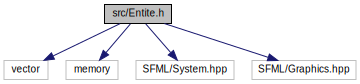
\includegraphics[width=350pt]{_entite_8h__incl}
\end{center}
\end{figure}
Ce graphe montre quels fichiers incluent directement ou indirectement ce fichier \+:\nopagebreak
\begin{figure}[H]
\begin{center}
\leavevmode
\includegraphics[width=350pt]{_entite_8h__dep__incl}
\end{center}
\end{figure}
\subsection*{Classes}
\begin{DoxyCompactItemize}
\item 
class \hyperlink{class_entite}{Entite}
\begin{DoxyCompactList}\small\item\em Classe virtuelle qui définit une entité \end{DoxyCompactList}\end{DoxyCompactItemize}

\hypertarget{bindings_8cpp}{}\section{Référence du fichier src/\+Interface/bindings.cpp}
\label{bindings_8cpp}\index{src/\+Interface/bindings.\+cpp@{src/\+Interface/bindings.\+cpp}}
{\ttfamily \#include \char`\"{}bindings.\+h\char`\"{}}\newline
Graphe des dépendances par inclusion de bindings.\+cpp\+:
% FIG 0
\subsection*{Fonctions}
\begin{DoxyCompactItemize}
\item 
void \hyperlink{bindings_8cpp_a17708a73bad94fe511a43e063956565d}{set\+\_\+keyboard\+\_\+default\+\_\+binding\+\_\+2} (\hyperlink{_input_8h_a5588d60d674991c719a8df848313e966}{Input} \&in)
\item 
void \hyperlink{bindings_8cpp_a33f9529428adfaa552e681749b796076}{set\+\_\+keyboard\+\_\+default\+\_\+binding} (\hyperlink{_input_8h_a5588d60d674991c719a8df848313e966}{Input} \&in)
\item 
void \hyperlink{bindings_8cpp_a6c343c7a09bb1d08e2a0f6e97773f57b}{set\+\_\+mouse\+\_\+default\+\_\+binding} (\hyperlink{_input_8h_a5588d60d674991c719a8df848313e966}{Input} \&in)
\item 
void \hyperlink{bindings_8cpp_a5249f510d79fb689561e3e4de1bba0d4}{set\+\_\+joypad\+\_\+default\+\_\+binding} (\hyperlink{_input_8h_a5588d60d674991c719a8df848313e966}{Input} \&in)
\end{DoxyCompactItemize}


\subsection{Documentation des fonctions}
\mbox{\Hypertarget{bindings_8cpp_a5249f510d79fb689561e3e4de1bba0d4}\label{bindings_8cpp_a5249f510d79fb689561e3e4de1bba0d4}} 
\index{bindings.\+cpp@{bindings.\+cpp}!set\+\_\+joypad\+\_\+default\+\_\+binding@{set\+\_\+joypad\+\_\+default\+\_\+binding}}
\index{set\+\_\+joypad\+\_\+default\+\_\+binding@{set\+\_\+joypad\+\_\+default\+\_\+binding}!bindings.\+cpp@{bindings.\+cpp}}
\subsubsection{\texorpdfstring{set\+\_\+joypad\+\_\+default\+\_\+binding()}{set\_joypad\_default\_binding()}}
{\footnotesize\ttfamily void set\+\_\+joypad\+\_\+default\+\_\+binding (\begin{DoxyParamCaption}\item[{\hyperlink{_input_8h_a5588d60d674991c719a8df848313e966}{Input} \&}]{in }\end{DoxyParamCaption})}

\mbox{\Hypertarget{bindings_8cpp_a33f9529428adfaa552e681749b796076}\label{bindings_8cpp_a33f9529428adfaa552e681749b796076}} 
\index{bindings.\+cpp@{bindings.\+cpp}!set\+\_\+keyboard\+\_\+default\+\_\+binding@{set\+\_\+keyboard\+\_\+default\+\_\+binding}}
\index{set\+\_\+keyboard\+\_\+default\+\_\+binding@{set\+\_\+keyboard\+\_\+default\+\_\+binding}!bindings.\+cpp@{bindings.\+cpp}}
\subsubsection{\texorpdfstring{set\+\_\+keyboard\+\_\+default\+\_\+binding()}{set\_keyboard\_default\_binding()}}
{\footnotesize\ttfamily void set\+\_\+keyboard\+\_\+default\+\_\+binding (\begin{DoxyParamCaption}\item[{\hyperlink{_input_8h_a5588d60d674991c719a8df848313e966}{Input} \&}]{in }\end{DoxyParamCaption})}

\mbox{\Hypertarget{bindings_8cpp_a17708a73bad94fe511a43e063956565d}\label{bindings_8cpp_a17708a73bad94fe511a43e063956565d}} 
\index{bindings.\+cpp@{bindings.\+cpp}!set\+\_\+keyboard\+\_\+default\+\_\+binding\+\_\+2@{set\+\_\+keyboard\+\_\+default\+\_\+binding\+\_\+2}}
\index{set\+\_\+keyboard\+\_\+default\+\_\+binding\+\_\+2@{set\+\_\+keyboard\+\_\+default\+\_\+binding\+\_\+2}!bindings.\+cpp@{bindings.\+cpp}}
\subsubsection{\texorpdfstring{set\+\_\+keyboard\+\_\+default\+\_\+binding\+\_\+2()}{set\_keyboard\_default\_binding\_2()}}
{\footnotesize\ttfamily void set\+\_\+keyboard\+\_\+default\+\_\+binding\+\_\+2 (\begin{DoxyParamCaption}\item[{\hyperlink{_input_8h_a5588d60d674991c719a8df848313e966}{Input} \&}]{in }\end{DoxyParamCaption})}

\mbox{\Hypertarget{bindings_8cpp_a6c343c7a09bb1d08e2a0f6e97773f57b}\label{bindings_8cpp_a6c343c7a09bb1d08e2a0f6e97773f57b}} 
\index{bindings.\+cpp@{bindings.\+cpp}!set\+\_\+mouse\+\_\+default\+\_\+binding@{set\+\_\+mouse\+\_\+default\+\_\+binding}}
\index{set\+\_\+mouse\+\_\+default\+\_\+binding@{set\+\_\+mouse\+\_\+default\+\_\+binding}!bindings.\+cpp@{bindings.\+cpp}}
\subsubsection{\texorpdfstring{set\+\_\+mouse\+\_\+default\+\_\+binding()}{set\_mouse\_default\_binding()}}
{\footnotesize\ttfamily void set\+\_\+mouse\+\_\+default\+\_\+binding (\begin{DoxyParamCaption}\item[{\hyperlink{_input_8h_a5588d60d674991c719a8df848313e966}{Input} \&}]{in }\end{DoxyParamCaption})}


\hypertarget{bindings_8h}{}\section{src/\+Interface/bindings.h File Reference}
\label{bindings_8h}\index{src/\+Interface/bindings.\+h@{src/\+Interface/bindings.\+h}}
{\ttfamily \#include \char`\"{}Input.\+h\char`\"{}}\newline
\subsection*{Functions}
\begin{DoxyCompactItemize}
\item 
void \mbox{\hyperlink{bindings_8h_a33f9529428adfaa552e681749b796076}{set\+\_\+keyboard\+\_\+default\+\_\+binding}} (\mbox{\hyperlink{_input_8h_a5588d60d674991c719a8df848313e966}{Input}} \&in)
\item 
void \mbox{\hyperlink{bindings_8h_a17708a73bad94fe511a43e063956565d}{set\+\_\+keyboard\+\_\+default\+\_\+binding\+\_\+2}} (\mbox{\hyperlink{_input_8h_a5588d60d674991c719a8df848313e966}{Input}} \&in)
\item 
void \mbox{\hyperlink{bindings_8h_a6c343c7a09bb1d08e2a0f6e97773f57b}{set\+\_\+mouse\+\_\+default\+\_\+binding}} (\mbox{\hyperlink{_input_8h_a5588d60d674991c719a8df848313e966}{Input}} \&in)
\item 
void \mbox{\hyperlink{bindings_8h_a5249f510d79fb689561e3e4de1bba0d4}{set\+\_\+joypad\+\_\+default\+\_\+binding}} (\mbox{\hyperlink{_input_8h_a5588d60d674991c719a8df848313e966}{Input}} \&in)
\end{DoxyCompactItemize}


\subsection{Function Documentation}
\mbox{\Hypertarget{bindings_8h_a5249f510d79fb689561e3e4de1bba0d4}\label{bindings_8h_a5249f510d79fb689561e3e4de1bba0d4}} 
\index{bindings.\+h@{bindings.\+h}!set\+\_\+joypad\+\_\+default\+\_\+binding@{set\+\_\+joypad\+\_\+default\+\_\+binding}}
\index{set\+\_\+joypad\+\_\+default\+\_\+binding@{set\+\_\+joypad\+\_\+default\+\_\+binding}!bindings.\+h@{bindings.\+h}}
\subsubsection{\texorpdfstring{set\+\_\+joypad\+\_\+default\+\_\+binding()}{set\_joypad\_default\_binding()}}
{\footnotesize\ttfamily void set\+\_\+joypad\+\_\+default\+\_\+binding (\begin{DoxyParamCaption}\item[{\mbox{\hyperlink{_input_8h_a5588d60d674991c719a8df848313e966}{Input}} \&}]{in }\end{DoxyParamCaption})}

\mbox{\Hypertarget{bindings_8h_a33f9529428adfaa552e681749b796076}\label{bindings_8h_a33f9529428adfaa552e681749b796076}} 
\index{bindings.\+h@{bindings.\+h}!set\+\_\+keyboard\+\_\+default\+\_\+binding@{set\+\_\+keyboard\+\_\+default\+\_\+binding}}
\index{set\+\_\+keyboard\+\_\+default\+\_\+binding@{set\+\_\+keyboard\+\_\+default\+\_\+binding}!bindings.\+h@{bindings.\+h}}
\subsubsection{\texorpdfstring{set\+\_\+keyboard\+\_\+default\+\_\+binding()}{set\_keyboard\_default\_binding()}}
{\footnotesize\ttfamily void set\+\_\+keyboard\+\_\+default\+\_\+binding (\begin{DoxyParamCaption}\item[{\mbox{\hyperlink{_input_8h_a5588d60d674991c719a8df848313e966}{Input}} \&}]{in }\end{DoxyParamCaption})}

\mbox{\Hypertarget{bindings_8h_a17708a73bad94fe511a43e063956565d}\label{bindings_8h_a17708a73bad94fe511a43e063956565d}} 
\index{bindings.\+h@{bindings.\+h}!set\+\_\+keyboard\+\_\+default\+\_\+binding\+\_\+2@{set\+\_\+keyboard\+\_\+default\+\_\+binding\+\_\+2}}
\index{set\+\_\+keyboard\+\_\+default\+\_\+binding\+\_\+2@{set\+\_\+keyboard\+\_\+default\+\_\+binding\+\_\+2}!bindings.\+h@{bindings.\+h}}
\subsubsection{\texorpdfstring{set\+\_\+keyboard\+\_\+default\+\_\+binding\+\_\+2()}{set\_keyboard\_default\_binding\_2()}}
{\footnotesize\ttfamily void set\+\_\+keyboard\+\_\+default\+\_\+binding\+\_\+2 (\begin{DoxyParamCaption}\item[{\mbox{\hyperlink{_input_8h_a5588d60d674991c719a8df848313e966}{Input}} \&}]{in }\end{DoxyParamCaption})}

\mbox{\Hypertarget{bindings_8h_a6c343c7a09bb1d08e2a0f6e97773f57b}\label{bindings_8h_a6c343c7a09bb1d08e2a0f6e97773f57b}} 
\index{bindings.\+h@{bindings.\+h}!set\+\_\+mouse\+\_\+default\+\_\+binding@{set\+\_\+mouse\+\_\+default\+\_\+binding}}
\index{set\+\_\+mouse\+\_\+default\+\_\+binding@{set\+\_\+mouse\+\_\+default\+\_\+binding}!bindings.\+h@{bindings.\+h}}
\subsubsection{\texorpdfstring{set\+\_\+mouse\+\_\+default\+\_\+binding()}{set\_mouse\_default\_binding()}}
{\footnotesize\ttfamily void set\+\_\+mouse\+\_\+default\+\_\+binding (\begin{DoxyParamCaption}\item[{\mbox{\hyperlink{_input_8h_a5588d60d674991c719a8df848313e966}{Input}} \&}]{in }\end{DoxyParamCaption})}


\hypertarget{_bouton_capacite_8h}{}\section{src/\+Interface/\+Bouton\+Capacite.h File Reference}
\label{_bouton_capacite_8h}\index{src/\+Interface/\+Bouton\+Capacite.\+h@{src/\+Interface/\+Bouton\+Capacite.\+h}}
\subsection*{Classes}
\begin{DoxyCompactItemize}
\item 
class \mbox{\hyperlink{class_bouton_capacite}{Bouton\+Capacite}}
\end{DoxyCompactItemize}

\hypertarget{_input_8cpp}{}\section{Référence du fichier src/\+Interface/\+Input.cpp}
\label{_input_8cpp}\index{src/\+Interface/\+Input.\+cpp@{src/\+Interface/\+Input.\+cpp}}
{\ttfamily \#include \char`\"{}Input.\+h\char`\"{}}\newline
{\ttfamily \#include $<$cmath$>$}\newline
Graphe des dépendances par inclusion de Input.\+cpp\+:\nopagebreak
\begin{figure}[H]
\begin{center}
\leavevmode
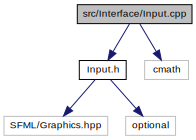
\includegraphics[width=269pt]{_input_8cpp__incl}
\end{center}
\end{figure}

\hypertarget{_input_8h}{}\section{Référence du fichier src/\+Interface/\+Input.h}
\label{_input_8h}\index{src/\+Interface/\+Input.\+h@{src/\+Interface/\+Input.\+h}}
{\ttfamily \#include $<$S\+F\+M\+L/\+Graphics.\+hpp$>$}\newline
{\ttfamily \#include $<$bitset$>$}\newline
{\ttfamily \#include \char`\"{}../constantes.\+h\char`\"{}}\newline
{\ttfamily \#include \char`\"{}../\+Utilitaires/optional.\+h\char`\"{}}\newline
Graphe des dépendances par inclusion de Input.\+h\+:
% FIG 0
Ce graphe montre quels fichiers incluent directement ou indirectement ce fichier \+:
% FIG 1
\subsection*{Classes}
\begin{DoxyCompactItemize}
\item 
class \hyperlink{class_input__base}{Input\+\_\+base$<$ N $>$}
\end{DoxyCompactItemize}
\subsection*{Définitions de type}
\begin{DoxyCompactItemize}
\item 
using \hyperlink{_input_8h_a5588d60d674991c719a8df848313e966}{Input} = \hyperlink{class_input__base}{Input\+\_\+base}$<$ \hyperlink{constantes_8h_a726db5d0e2803e025a8677641c60887b}{N\+B\+\_\+\+A\+C\+T\+I\+ON} $>$
\end{DoxyCompactItemize}


\subsection{Documentation des définitions de type}
\mbox{\Hypertarget{_input_8h_a5588d60d674991c719a8df848313e966}\label{_input_8h_a5588d60d674991c719a8df848313e966}} 
\index{Input.\+h@{Input.\+h}!Input@{Input}}
\index{Input@{Input}!Input.\+h@{Input.\+h}}
\subsubsection{\texorpdfstring{Input}{Input}}
{\footnotesize\ttfamily using \hyperlink{_input_8h_a5588d60d674991c719a8df848313e966}{Input} =  \hyperlink{class_input__base}{Input\+\_\+base}$<$\hyperlink{constantes_8h_a726db5d0e2803e025a8677641c60887b}{N\+B\+\_\+\+A\+C\+T\+I\+ON}$>$}


\hypertarget{_overlay_8cpp}{}\section{src/\+Interface/\+Overlay.cpp File Reference}
\label{_overlay_8cpp}\index{src/\+Interface/\+Overlay.\+cpp@{src/\+Interface/\+Overlay.\+cpp}}
{\ttfamily \#include \char`\"{}Overlay.\+h\char`\"{}}\newline

\hypertarget{_overlay_8h}{}\section{src/\+Interface/\+Overlay.h File Reference}
\label{_overlay_8h}\index{src/\+Interface/\+Overlay.\+h@{src/\+Interface/\+Overlay.\+h}}
{\ttfamily \#include \char`\"{}S\+F\+M\+L/\+Graphics.\+hpp\char`\"{}}\newline
{\ttfamily \#include \char`\"{}../constantes.\+h\char`\"{}}\newline
{\ttfamily \#include \char`\"{}../\+Vaisseau/\+Vaisseau.\+h\char`\"{}}\newline
{\ttfamily \#include \char`\"{}../def\+\_\+type.\+h\char`\"{}}\newline
{\ttfamily \#include $<$iostream$>$}\newline
\subsection*{Classes}
\begin{DoxyCompactItemize}
\item 
class \mbox{\hyperlink{class_overlay}{Overlay}}
\begin{DoxyCompactList}\small\item\em Classe qui le bouton des capacité IG. \end{DoxyCompactList}\end{DoxyCompactItemize}

\hypertarget{main_8cpp}{}\section{Référence du fichier src/main.cpp}
\label{main_8cpp}\index{src/main.\+cpp@{src/main.\+cpp}}
{\ttfamily \#include $<$S\+F\+M\+L/\+Graphics.\+hpp$>$}\newline
{\ttfamily \#include $<$cmath$>$}\newline
{\ttfamily \#include $<$ctime$>$}\newline
{\ttfamily \#include $<$iostream$>$}\newline
{\ttfamily \#include \char`\"{}constantes.\+h\char`\"{}}\newline
{\ttfamily \#include \char`\"{}Entite.\+h\char`\"{}}\newline
{\ttfamily \#include \char`\"{}Utilitaires/\+Collision.\+h\char`\"{}}\newline
{\ttfamily \#include \char`\"{}Partie.\+h\char`\"{}}\newline
Graphe des dépendances par inclusion de main.\+cpp\+:\nopagebreak
\begin{figure}[H]
\begin{center}
\leavevmode
\includegraphics[width=350pt]{main_8cpp__incl}
\end{center}
\end{figure}
\subsection*{Fonctions}
\begin{DoxyCompactItemize}
\item 
int \hyperlink{main_8cpp_ae66f6b31b5ad750f1fe042a706a4e3d4}{main} ()
\end{DoxyCompactItemize}


\subsection{Documentation des fonctions}
\mbox{\Hypertarget{main_8cpp_ae66f6b31b5ad750f1fe042a706a4e3d4}\label{main_8cpp_ae66f6b31b5ad750f1fe042a706a4e3d4}} 
\index{main.\+cpp@{main.\+cpp}!main@{main}}
\index{main@{main}!main.\+cpp@{main.\+cpp}}
\subsubsection{\texorpdfstring{main()}{main()}}
{\footnotesize\ttfamily int main (\begin{DoxyParamCaption}{ }\end{DoxyParamCaption})}

le truc que Cyril avait tapé jeudi 7 en club

$<$attention très bordélique 
\hypertarget{_accueil_8cpp}{}\section{src/\+Menu/\+Accueil.cpp File Reference}
\label{_accueil_8cpp}\index{src/\+Menu/\+Accueil.\+cpp@{src/\+Menu/\+Accueil.\+cpp}}
{\ttfamily \#include \char`\"{}Accueil.\+h\char`\"{}}\newline

\hypertarget{_accueil_8h}{}\section{src/\+Menu/\+Accueil.h File Reference}
\label{_accueil_8h}\index{src/\+Menu/\+Accueil.\+h@{src/\+Menu/\+Accueil.\+h}}
{\ttfamily \#include \char`\"{}Ecran.\+h\char`\"{}}\newline
\subsection*{Classes}
\begin{DoxyCompactItemize}
\item 
class \mbox{\hyperlink{class_accueil}{Accueil}}
\end{DoxyCompactItemize}

\hypertarget{_ecran_8cpp}{}\section{src/\+Menu/\+Ecran.cpp File Reference}
\label{_ecran_8cpp}\index{src/\+Menu/\+Ecran.\+cpp@{src/\+Menu/\+Ecran.\+cpp}}
{\ttfamily \#include \char`\"{}Ecran.\+h\char`\"{}}\newline
\subsection*{Functions}
\begin{DoxyCompactItemize}
\item 
void \mbox{\hyperlink{_ecran_8cpp_a302f2585a4c0c94fd4db6106ecf02441}{chargement}} (sf\+::\+Render\+Window \&window, sf\+::\+Texture \&derniere\+Fenetre)
\end{DoxyCompactItemize}


\subsection{Function Documentation}
\mbox{\Hypertarget{_ecran_8cpp_a302f2585a4c0c94fd4db6106ecf02441}\label{_ecran_8cpp_a302f2585a4c0c94fd4db6106ecf02441}} 
\index{Ecran.\+cpp@{Ecran.\+cpp}!chargement@{chargement}}
\index{chargement@{chargement}!Ecran.\+cpp@{Ecran.\+cpp}}
\subsubsection{\texorpdfstring{chargement()}{chargement()}}
{\footnotesize\ttfamily void chargement (\begin{DoxyParamCaption}\item[{sf\+::\+Render\+Window \&}]{window,  }\item[{sf\+::\+Texture \&}]{derniere\+Fenetre }\end{DoxyParamCaption})}


\hypertarget{_ecran_8h}{}\section{src/\+Menu/\+Ecran.h File Reference}
\label{_ecran_8h}\index{src/\+Menu/\+Ecran.\+h@{src/\+Menu/\+Ecran.\+h}}
{\ttfamily \#include \char`\"{}../constantes.\+h\char`\"{}}\newline
{\ttfamily \#include \char`\"{}../def\+\_\+type.\+h\char`\"{}}\newline
{\ttfamily \#include \char`\"{}../\+Utilitaires/optional.\+h\char`\"{}}\newline
{\ttfamily \#include \char`\"{}../\+Utilitaires/\+Chargeur.\+h\char`\"{}}\newline
{\ttfamily \#include $<$stack$>$}\newline
{\ttfamily \#include $<$memory$>$}\newline
{\ttfamily \#include $<$vector$>$}\newline
{\ttfamily \#include $<$map$>$}\newline
{\ttfamily \#include $<$S\+F\+M\+L/\+System.\+hpp$>$}\newline
{\ttfamily \#include $<$S\+F\+M\+L/\+Graphics.\+hpp$>$}\newline
{\ttfamily \#include $<$S\+F\+M\+L/\+Audio.\+hpp$>$}\newline
\subsection*{Classes}
\begin{DoxyCompactItemize}
\item 
class \mbox{\hyperlink{class_ecran}{Ecran}}
\end{DoxyCompactItemize}
\subsection*{Functions}
\begin{DoxyCompactItemize}
\item 
void \mbox{\hyperlink{_ecran_8h_a302f2585a4c0c94fd4db6106ecf02441}{chargement}} (sf\+::\+Render\+Window \&window, sf\+::\+Texture \&derniere\+Fenetre)
\end{DoxyCompactItemize}


\subsection{Function Documentation}
\mbox{\Hypertarget{_ecran_8h_a302f2585a4c0c94fd4db6106ecf02441}\label{_ecran_8h_a302f2585a4c0c94fd4db6106ecf02441}} 
\index{Ecran.\+h@{Ecran.\+h}!chargement@{chargement}}
\index{chargement@{chargement}!Ecran.\+h@{Ecran.\+h}}
\subsubsection{\texorpdfstring{chargement()}{chargement()}}
{\footnotesize\ttfamily void chargement (\begin{DoxyParamCaption}\item[{sf\+::\+Render\+Window \&}]{window,  }\item[{sf\+::\+Texture \&}]{derniere\+Fenetre }\end{DoxyParamCaption})}


\hypertarget{_menu_principal_8cpp}{}\section{src/\+Menu/\+Menu\+Principal.cpp File Reference}
\label{_menu_principal_8cpp}\index{src/\+Menu/\+Menu\+Principal.\+cpp@{src/\+Menu/\+Menu\+Principal.\+cpp}}
{\ttfamily \#include \char`\"{}Menu\+Principal.\+h\char`\"{}}\newline

\hypertarget{_menu_principal_8h}{}\section{src/\+Menu/\+Menu\+Principal.h File Reference}
\label{_menu_principal_8h}\index{src/\+Menu/\+Menu\+Principal.\+h@{src/\+Menu/\+Menu\+Principal.\+h}}
{\ttfamily \#include \char`\"{}Ecran.\+h\char`\"{}}\newline
\subsection*{Classes}
\begin{DoxyCompactItemize}
\item 
class \mbox{\hyperlink{class_menu_principal}{Menu\+Principal}}
\end{DoxyCompactItemize}

\hypertarget{_partie_8cpp}{}\section{Référence du fichier src/\+Partie.cpp}
\label{_partie_8cpp}\index{src/\+Partie.\+cpp@{src/\+Partie.\+cpp}}
{\ttfamily \#include \char`\"{}Partie.\+h\char`\"{}}\newline
{\ttfamily \#include \char`\"{}\+\_\+projectiles.\+h\char`\"{}}\newline
{\ttfamily \#include \char`\"{}\+\_\+\+Capacites.\+h\char`\"{}}\newline
{\ttfamily \#include \char`\"{}Proj\+Test.\+h\char`\"{}}\newline
{\ttfamily \#include \char`\"{}Vaisseau\+Test.\+h\char`\"{}}\newline
Graphe des dépendances par inclusion de Partie.\+cpp\+:\nopagebreak
\begin{figure}[H]
\begin{center}
\leavevmode
\includegraphics[width=350pt]{_partie_8cpp__incl}
\end{center}
\end{figure}

\hypertarget{_partie_8h}{}\section{Référence du fichier src/\+Partie.h}
\label{_partie_8h}\index{src/\+Partie.\+h@{src/\+Partie.\+h}}
{\ttfamily \#include $<$vector$>$}\newline
{\ttfamily \#include $<$string$>$}\newline
{\ttfamily \#include $<$algorithm$>$}\newline
{\ttfamily \#include \char`\"{}Capacite.\+h\char`\"{}}\newline
{\ttfamily \#include \char`\"{}Projectile.\+h\char`\"{}}\newline
{\ttfamily \#include \char`\"{}Vaisseau.\+h\char`\"{}}\newline
Graphe des dépendances par inclusion de Partie.\+h\+:\nopagebreak
\begin{figure}[H]
\begin{center}
\leavevmode
\includegraphics[width=323pt]{_partie_8h__incl}
\end{center}
\end{figure}
\subsection*{Classes}
\begin{DoxyCompactItemize}
\item 
class \hyperlink{class_partie}{Partie}
\begin{DoxyCompactList}\small\item\em Description brève. \end{DoxyCompactList}\end{DoxyCompactItemize}

\hypertarget{_pattern_8cpp}{}\section{src/\+Pattern/\+Pattern.cpp File Reference}
\label{_pattern_8cpp}\index{src/\+Pattern/\+Pattern.\+cpp@{src/\+Pattern/\+Pattern.\+cpp}}
{\ttfamily \#include \char`\"{}Pattern.\+h\char`\"{}}\newline

\hypertarget{_pattern_8h}{}\section{Référence du fichier src/\+Pattern/\+Pattern.h}
\label{_pattern_8h}\index{src/\+Pattern/\+Pattern.\+h@{src/\+Pattern/\+Pattern.\+h}}
{\ttfamily \#include \char`\"{}Vague.\+h\char`\"{}}\newline
{\ttfamily \#include \char`\"{}../\+Partie.\+h\char`\"{}}\newline
Graphe des dépendances par inclusion de Pattern.\+h\+:
% FIG 0
Ce graphe montre quels fichiers incluent directement ou indirectement ce fichier \+:
% FIG 1
\subsection*{Classes}
\begin{DoxyCompactItemize}
\item 
class \hyperlink{class_pattern}{Pattern}
\end{DoxyCompactItemize}

\hypertarget{_vague_8cpp}{}\section{Référence du fichier src/\+Pattern/\+Vague.cpp}
\label{_vague_8cpp}\index{src/\+Pattern/\+Vague.\+cpp@{src/\+Pattern/\+Vague.\+cpp}}
{\ttfamily \#include \char`\"{}Vague.\+h\char`\"{}}\newline
Graphe des dépendances par inclusion de Vague.\+cpp\+:
% FIG 0

\hypertarget{_vague_8h}{}\section{src/\+Pattern/\+Vague.h File Reference}
\label{_vague_8h}\index{src/\+Pattern/\+Vague.\+h@{src/\+Pattern/\+Vague.\+h}}
{\ttfamily \#include $<$vector$>$}\newline
{\ttfamily \#include $<$S\+F\+M\+L/\+Graphics.\+hpp$>$}\newline
{\ttfamily \#include \char`\"{}../\+Vaisseau/\+\_\+vaisseaux.\+h\char`\"{}}\newline
{\ttfamily \#include \char`\"{}../def\+\_\+type.\+h\char`\"{}}\newline
\subsection*{Classes}
\begin{DoxyCompactItemize}
\item 
struct \mbox{\hyperlink{struct_element_vague}{Element\+Vague}}
\item 
class \mbox{\hyperlink{class_vague}{Vague}}
\begin{DoxyCompactList}\small\item\em Classe qui décrit les vagues d\textquotesingle{}ennemis. \end{DoxyCompactList}\end{DoxyCompactItemize}

\hypertarget{__projectiles_8h}{}\section{src/\+Projectiles/\+\_\+projectiles.h File Reference}
\label{__projectiles_8h}\index{src/\+Projectiles/\+\_\+projectiles.\+h@{src/\+Projectiles/\+\_\+projectiles.\+h}}
{\ttfamily \#include \char`\"{}Proj\+Boing.\+h\char`\"{}}\newline
{\ttfamily \#include \char`\"{}Proj\+Piou.\+h\char`\"{}}\newline
{\ttfamily \#include \char`\"{}Proj\+Missile.\+h\char`\"{}}\newline
{\ttfamily \#include \char`\"{}Proj\+Bismillah.\+h\char`\"{}}\newline

\hypertarget{_proj_bismillah_8cpp}{}\section{src/\+Projectiles/\+Proj\+Bismillah.cpp File Reference}
\label{_proj_bismillah_8cpp}\index{src/\+Projectiles/\+Proj\+Bismillah.\+cpp@{src/\+Projectiles/\+Proj\+Bismillah.\+cpp}}
{\ttfamily \#include \char`\"{}Proj\+Bismillah.\+h\char`\"{}}\newline
{\ttfamily \#include $<$cmath$>$}\newline

\hypertarget{_proj_bismillah_8h}{}\section{Référence du fichier src/\+Projectiles/\+Proj\+Bismillah.h}
\label{_proj_bismillah_8h}\index{src/\+Projectiles/\+Proj\+Bismillah.\+h@{src/\+Projectiles/\+Proj\+Bismillah.\+h}}
{\ttfamily \#include \char`\"{}Projectile.\+h\char`\"{}}\newline
Graphe des dépendances par inclusion de Proj\+Bismillah.\+h\+:
% FIG 0
Ce graphe montre quels fichiers incluent directement ou indirectement ce fichier \+:
% FIG 1
\subsection*{Classes}
\begin{DoxyCompactItemize}
\item 
class \hyperlink{class_proj_bismillah}{Proj\+Bismillah}
\end{DoxyCompactItemize}

\hypertarget{_proj_boing_8cpp}{}\section{Référence du fichier src/\+Projectiles/\+Proj\+Boing.cpp}
\label{_proj_boing_8cpp}\index{src/\+Projectiles/\+Proj\+Boing.\+cpp@{src/\+Projectiles/\+Proj\+Boing.\+cpp}}
{\ttfamily \#include \char`\"{}Proj\+Boing.\+h\char`\"{}}\newline
{\ttfamily \#include \char`\"{}../constantes.\+h\char`\"{}}\newline
Graphe des dépendances par inclusion de Proj\+Boing.\+cpp\+:
% FIG 0

\hypertarget{_proj_boing_8h}{}\section{src/\+Projectiles/\+Proj\+Boing.h File Reference}
\label{_proj_boing_8h}\index{src/\+Projectiles/\+Proj\+Boing.\+h@{src/\+Projectiles/\+Proj\+Boing.\+h}}
{\ttfamily \#include \char`\"{}Projectile.\+h\char`\"{}}\newline
\subsection*{Classes}
\begin{DoxyCompactItemize}
\item 
class \mbox{\hyperlink{class_proj_boing}{Proj\+Boing}}
\begin{DoxyCompactList}\small\item\em \mbox{\hyperlink{class_projectile}{Projectile}} de test. \end{DoxyCompactList}\end{DoxyCompactItemize}

\hypertarget{_proj_bouclier_rond_8cpp}{}\section{Référence du fichier src/\+Projectiles/\+Proj\+Bouclier\+Rond.cpp}
\label{_proj_bouclier_rond_8cpp}\index{src/\+Projectiles/\+Proj\+Bouclier\+Rond.\+cpp@{src/\+Projectiles/\+Proj\+Bouclier\+Rond.\+cpp}}
{\ttfamily \#include \char`\"{}Proj\+Bouclier\+Rond.\+h\char`\"{}}\newline
{\ttfamily \#include $<$cmath$>$}\newline
Graphe des dépendances par inclusion de Proj\+Bouclier\+Rond.\+cpp\+:
% FIG 0

\hypertarget{_proj_bouclier_rond_8h}{}\section{Référence du fichier src/\+Projectiles/\+Proj\+Bouclier\+Rond.h}
\label{_proj_bouclier_rond_8h}\index{src/\+Projectiles/\+Proj\+Bouclier\+Rond.\+h@{src/\+Projectiles/\+Proj\+Bouclier\+Rond.\+h}}
{\ttfamily \#include \char`\"{}Projectile.\+h\char`\"{}}\newline
Graphe des dépendances par inclusion de Proj\+Bouclier\+Rond.\+h\+:
% FIG 0
Ce graphe montre quels fichiers incluent directement ou indirectement ce fichier \+:
% FIG 1
\subsection*{Classes}
\begin{DoxyCompactItemize}
\item 
class \hyperlink{class_proj_bouclier_rond}{Proj\+Bouclier\+Rond}
\end{DoxyCompactItemize}

\hypertarget{_projectile_8cpp}{}\section{src/\+Projectiles/\+Projectile.cpp File Reference}
\label{_projectile_8cpp}\index{src/\+Projectiles/\+Projectile.\+cpp@{src/\+Projectiles/\+Projectile.\+cpp}}
{\ttfamily \#include \char`\"{}Projectile.\+h\char`\"{}}\newline
{\ttfamily \#include $<$climits$>$}\newline

\hypertarget{_projectile_8h}{}\section{Référence du fichier src/\+Projectiles/\+Projectile.h}
\label{_projectile_8h}\index{src/\+Projectiles/\+Projectile.\+h@{src/\+Projectiles/\+Projectile.\+h}}
{\ttfamily \#include $<$vector$>$}\newline
{\ttfamily \#include $<$string$>$}\newline
{\ttfamily \#include $<$algorithm$>$}\newline
{\ttfamily \#include \char`\"{}../\+Entite.\+h\char`\"{}}\newline
Graphe des dépendances par inclusion de Projectile.\+h\+:
% FIG 0
Ce graphe montre quels fichiers incluent directement ou indirectement ce fichier \+:
% FIG 1
\subsection*{Classes}
\begin{DoxyCompactItemize}
\item 
class \hyperlink{class_projectile}{Projectile}
\begin{DoxyCompactList}\small\item\em Classe abstraite qui définit la structure générale d\textquotesingle{}un projectile, à faire hériter pour chaque projectile. \end{DoxyCompactList}\end{DoxyCompactItemize}

\hypertarget{_proj_missile_8cpp}{}\section{src/\+Projectiles/\+Proj\+Missile.cpp File Reference}
\label{_proj_missile_8cpp}\index{src/\+Projectiles/\+Proj\+Missile.\+cpp@{src/\+Projectiles/\+Proj\+Missile.\+cpp}}
{\ttfamily \#include \char`\"{}Proj\+Missile.\+h\char`\"{}}\newline
{\ttfamily \#include $<$cmath$>$}\newline

\hypertarget{_proj_missile_8h}{}\section{Référence du fichier src/\+Projectiles/\+Proj\+Missile.h}
\label{_proj_missile_8h}\index{src/\+Projectiles/\+Proj\+Missile.\+h@{src/\+Projectiles/\+Proj\+Missile.\+h}}
{\ttfamily \#include \char`\"{}Projectile.\+h\char`\"{}}\newline
Graphe des dépendances par inclusion de Proj\+Missile.\+h\+:
% FIG 0
Ce graphe montre quels fichiers incluent directement ou indirectement ce fichier \+:
% FIG 1
\subsection*{Classes}
\begin{DoxyCompactItemize}
\item 
class \hyperlink{class_proj_missile}{Proj\+Missile}
\end{DoxyCompactItemize}

\hypertarget{_proj_piou_8cpp}{}\section{Référence du fichier src/\+Projectiles/\+Proj\+Piou.cpp}
\label{_proj_piou_8cpp}\index{src/\+Projectiles/\+Proj\+Piou.\+cpp@{src/\+Projectiles/\+Proj\+Piou.\+cpp}}
{\ttfamily \#include \char`\"{}Proj\+Piou.\+h\char`\"{}}\newline
{\ttfamily \#include $<$cmath$>$}\newline
Graphe des dépendances par inclusion de Proj\+Piou.\+cpp\+:
% FIG 0

\hypertarget{_proj_piou_8h}{}\section{Référence du fichier src/\+Projectiles/\+Proj\+Piou.h}
\label{_proj_piou_8h}\index{src/\+Projectiles/\+Proj\+Piou.\+h@{src/\+Projectiles/\+Proj\+Piou.\+h}}
{\ttfamily \#include \char`\"{}Projectile.\+h\char`\"{}}\newline
Graphe des dépendances par inclusion de Proj\+Piou.\+h\+:
\nopagebreak
\begin{figure}[H]
\begin{center}
\leavevmode
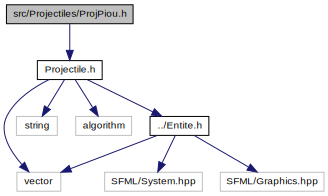
\includegraphics[width=350pt]{_proj_piou_8h__incl}
\end{center}
\end{figure}
Ce graphe montre quels fichiers incluent directement ou indirectement ce fichier \+:
\nopagebreak
\begin{figure}[H]
\begin{center}
\leavevmode
\includegraphics[width=350pt]{_proj_piou_8h__dep__incl}
\end{center}
\end{figure}
\subsection*{Classes}
\begin{DoxyCompactItemize}
\item 
class \hyperlink{class_proj_piou}{Proj\+Piou}
\end{DoxyCompactItemize}

\hypertarget{_chargeur_8cpp}{}\section{src/\+Utilitaires/\+Chargeur.cpp File Reference}
\label{_chargeur_8cpp}\index{src/\+Utilitaires/\+Chargeur.\+cpp@{src/\+Utilitaires/\+Chargeur.\+cpp}}
{\ttfamily \#include \char`\"{}Chargeur.\+h\char`\"{}}\newline
{\ttfamily \#include \char`\"{}../constantes.\+h\char`\"{}}\newline
{\ttfamily \#include \char`\"{}Divers.\+h\char`\"{}}\newline
{\ttfamily \#include $<$fstream$>$}\newline
{\ttfamily \#include $<$cctype$>$}\newline
{\ttfamily \#include $<$iostream$>$}\newline
{\ttfamily \#include $<$algorithm$>$}\newline

\hypertarget{_chargeur_8h}{}\section{src/\+Utilitaires/\+Chargeur.h File Reference}
\label{_chargeur_8h}\index{src/\+Utilitaires/\+Chargeur.\+h@{src/\+Utilitaires/\+Chargeur.\+h}}
{\ttfamily \#include \char`\"{}optional.\+h\char`\"{}}\newline
{\ttfamily \#include $<$memory$>$}\newline
{\ttfamily \#include $<$S\+F\+M\+L/\+Graphics.\+hpp$>$}\newline
{\ttfamily \#include $<$map$>$}\newline
{\ttfamily \#include $<$string$>$}\newline
{\ttfamily \#include $<$S\+F\+M\+L/\+Audio.\+hpp$>$}\newline
\subsection*{Classes}
\begin{DoxyCompactItemize}
\item 
struct \mbox{\hyperlink{structcase_insensitive_compare}{case\+Insensitive\+Compare}}
\item 
class \mbox{\hyperlink{class_chargeur}{Chargeur}}
\end{DoxyCompactItemize}

\hypertarget{_collision_8cpp}{}\section{Référence du fichier src/\+Utilitaires/\+Collision.cpp}
\label{_collision_8cpp}\index{src/\+Utilitaires/\+Collision.\+cpp@{src/\+Utilitaires/\+Collision.\+cpp}}
{\ttfamily \#include \char`\"{}Collision.\+h\char`\"{}}\newline
{\ttfamily \#include $<$cmath$>$}\newline
Graphe des dépendances par inclusion de Collision.\+cpp\+:\nopagebreak
\begin{figure}[H]
\begin{center}
\leavevmode
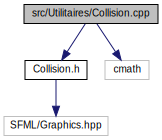
\includegraphics[width=234pt]{_collision_8cpp__incl}
\end{center}
\end{figure}
\subsection*{Fonctions}
\begin{DoxyCompactItemize}
\item 
sf\+::\+Vector2f \hyperlink{_collision_8cpp_a19be16a0d78cc53699ec1f6cc1247f0a}{centre\+\_\+transforme} (const sf\+::\+Circle\+Shape \&c)
\item 
sf\+::\+Vector2f \hyperlink{_collision_8cpp_aaf8f0e4613fb5a09397a7825b1ff4909}{point\+\_\+transforme} (const sf\+::\+Shape \&s, size\+\_\+t index)
\item 
bool \hyperlink{_collision_8cpp_a55cd5d990d317edd263c1d3bcd0b5a05}{is\+\_\+point\+\_\+in} (const sf\+::\+Vector2f \&C, const sf\+::\+Shape \&s)
\item 
bool \hyperlink{_collision_8cpp_a9037d2ebead3fc780ff50019012ac010}{collision} (const sf\+::\+Shape \&s1, const sf\+::\+Shape \&s2)
\item 
bool \hyperlink{_collision_8cpp_a4a4d2e91bbfd88f8aaaeb1572140a024}{collision\+\_\+impl} (const sf\+::\+Circle\+Shape \&c1, const sf\+::\+Circle\+Shape \&c2)
\item 
bool \hyperlink{_collision_8cpp_a598969c4bf7355123d972d3cf69eafd5}{collision\+\_\+impl} (const sf\+::\+Circle\+Shape \&c, const sf\+::\+Shape \&co)
\item 
bool \hyperlink{_collision_8cpp_adcae147b4b5b0ca770cfbc5b1c65873d}{collision\+\_\+impl} (const sf\+::\+Shape \&co, const sf\+::\+Circle\+Shape \&c)
\item 
bool \hyperlink{_collision_8cpp_ad5b149f81d5c820b0f81e5ca66385dee}{collision\+\_\+impl} (const sf\+::\+Shape \&s1, const sf\+::\+Shape \&s2)
\end{DoxyCompactItemize}
\subsection*{Variables}
\begin{DoxyCompactItemize}
\item 
const double \hyperlink{_collision_8cpp_a952eac791b596a61bba0a133a3bb439f}{PI} = acos(-\/1)
\end{DoxyCompactItemize}


\subsection{Documentation des fonctions}
\mbox{\Hypertarget{_collision_8cpp_a19be16a0d78cc53699ec1f6cc1247f0a}\label{_collision_8cpp_a19be16a0d78cc53699ec1f6cc1247f0a}} 
\index{Collision.\+cpp@{Collision.\+cpp}!centre\+\_\+transforme@{centre\+\_\+transforme}}
\index{centre\+\_\+transforme@{centre\+\_\+transforme}!Collision.\+cpp@{Collision.\+cpp}}
\subsubsection{\texorpdfstring{centre\+\_\+transforme()}{centre\_transforme()}}
{\footnotesize\ttfamily sf\+::\+Vector2f centre\+\_\+transforme (\begin{DoxyParamCaption}\item[{const sf\+::\+Circle\+Shape \&}]{c }\end{DoxyParamCaption})}

\mbox{\Hypertarget{_collision_8cpp_a9037d2ebead3fc780ff50019012ac010}\label{_collision_8cpp_a9037d2ebead3fc780ff50019012ac010}} 
\index{Collision.\+cpp@{Collision.\+cpp}!collision@{collision}}
\index{collision@{collision}!Collision.\+cpp@{Collision.\+cpp}}
\subsubsection{\texorpdfstring{collision()}{collision()}}
{\footnotesize\ttfamily bool collision (\begin{DoxyParamCaption}\item[{const sf\+::\+Shape \&}]{s1,  }\item[{const sf\+::\+Shape \&}]{s2 }\end{DoxyParamCaption})}

\mbox{\Hypertarget{_collision_8cpp_a4a4d2e91bbfd88f8aaaeb1572140a024}\label{_collision_8cpp_a4a4d2e91bbfd88f8aaaeb1572140a024}} 
\index{Collision.\+cpp@{Collision.\+cpp}!collision\+\_\+impl@{collision\+\_\+impl}}
\index{collision\+\_\+impl@{collision\+\_\+impl}!Collision.\+cpp@{Collision.\+cpp}}
\subsubsection{\texorpdfstring{collision\+\_\+impl()}{collision\_impl()}\hspace{0.1cm}{\footnotesize\ttfamily [1/4]}}
{\footnotesize\ttfamily bool collision\+\_\+impl (\begin{DoxyParamCaption}\item[{const sf\+::\+Circle\+Shape \&}]{c1,  }\item[{const sf\+::\+Circle\+Shape \&}]{c2 }\end{DoxyParamCaption})}

\mbox{\Hypertarget{_collision_8cpp_a598969c4bf7355123d972d3cf69eafd5}\label{_collision_8cpp_a598969c4bf7355123d972d3cf69eafd5}} 
\index{Collision.\+cpp@{Collision.\+cpp}!collision\+\_\+impl@{collision\+\_\+impl}}
\index{collision\+\_\+impl@{collision\+\_\+impl}!Collision.\+cpp@{Collision.\+cpp}}
\subsubsection{\texorpdfstring{collision\+\_\+impl()}{collision\_impl()}\hspace{0.1cm}{\footnotesize\ttfamily [2/4]}}
{\footnotesize\ttfamily bool collision\+\_\+impl (\begin{DoxyParamCaption}\item[{const sf\+::\+Circle\+Shape \&}]{c,  }\item[{const sf\+::\+Shape \&}]{co }\end{DoxyParamCaption})}

\mbox{\Hypertarget{_collision_8cpp_adcae147b4b5b0ca770cfbc5b1c65873d}\label{_collision_8cpp_adcae147b4b5b0ca770cfbc5b1c65873d}} 
\index{Collision.\+cpp@{Collision.\+cpp}!collision\+\_\+impl@{collision\+\_\+impl}}
\index{collision\+\_\+impl@{collision\+\_\+impl}!Collision.\+cpp@{Collision.\+cpp}}
\subsubsection{\texorpdfstring{collision\+\_\+impl()}{collision\_impl()}\hspace{0.1cm}{\footnotesize\ttfamily [3/4]}}
{\footnotesize\ttfamily bool collision\+\_\+impl (\begin{DoxyParamCaption}\item[{const sf\+::\+Shape \&}]{co,  }\item[{const sf\+::\+Circle\+Shape \&}]{c }\end{DoxyParamCaption})}

\mbox{\Hypertarget{_collision_8cpp_ad5b149f81d5c820b0f81e5ca66385dee}\label{_collision_8cpp_ad5b149f81d5c820b0f81e5ca66385dee}} 
\index{Collision.\+cpp@{Collision.\+cpp}!collision\+\_\+impl@{collision\+\_\+impl}}
\index{collision\+\_\+impl@{collision\+\_\+impl}!Collision.\+cpp@{Collision.\+cpp}}
\subsubsection{\texorpdfstring{collision\+\_\+impl()}{collision\_impl()}\hspace{0.1cm}{\footnotesize\ttfamily [4/4]}}
{\footnotesize\ttfamily bool collision\+\_\+impl (\begin{DoxyParamCaption}\item[{const sf\+::\+Shape \&}]{s1,  }\item[{const sf\+::\+Shape \&}]{s2 }\end{DoxyParamCaption})}

\mbox{\Hypertarget{_collision_8cpp_a55cd5d990d317edd263c1d3bcd0b5a05}\label{_collision_8cpp_a55cd5d990d317edd263c1d3bcd0b5a05}} 
\index{Collision.\+cpp@{Collision.\+cpp}!is\+\_\+point\+\_\+in@{is\+\_\+point\+\_\+in}}
\index{is\+\_\+point\+\_\+in@{is\+\_\+point\+\_\+in}!Collision.\+cpp@{Collision.\+cpp}}
\subsubsection{\texorpdfstring{is\+\_\+point\+\_\+in()}{is\_point\_in()}}
{\footnotesize\ttfamily bool is\+\_\+point\+\_\+in (\begin{DoxyParamCaption}\item[{const sf\+::\+Vector2f \&}]{C,  }\item[{const sf\+::\+Shape \&}]{s }\end{DoxyParamCaption})}

\mbox{\Hypertarget{_collision_8cpp_aaf8f0e4613fb5a09397a7825b1ff4909}\label{_collision_8cpp_aaf8f0e4613fb5a09397a7825b1ff4909}} 
\index{Collision.\+cpp@{Collision.\+cpp}!point\+\_\+transforme@{point\+\_\+transforme}}
\index{point\+\_\+transforme@{point\+\_\+transforme}!Collision.\+cpp@{Collision.\+cpp}}
\subsubsection{\texorpdfstring{point\+\_\+transforme()}{point\_transforme()}}
{\footnotesize\ttfamily sf\+::\+Vector2f point\+\_\+transforme (\begin{DoxyParamCaption}\item[{const sf\+::\+Shape \&}]{s,  }\item[{size\+\_\+t}]{index }\end{DoxyParamCaption})}



\subsection{Documentation des variables}
\mbox{\Hypertarget{_collision_8cpp_a952eac791b596a61bba0a133a3bb439f}\label{_collision_8cpp_a952eac791b596a61bba0a133a3bb439f}} 
\index{Collision.\+cpp@{Collision.\+cpp}!PI@{PI}}
\index{PI@{PI}!Collision.\+cpp@{Collision.\+cpp}}
\subsubsection{\texorpdfstring{PI}{PI}}
{\footnotesize\ttfamily const double PI = acos(-\/1)}


\hypertarget{_collision_8h}{}\section{Référence du fichier src/\+Collision.h}
\label{_collision_8h}\index{src/\+Collision.\+h@{src/\+Collision.\+h}}
{\ttfamily \#include $<$S\+F\+M\+L/\+Graphics.\+hpp$>$}\newline
Graphe des dépendances par inclusion de Collision.\+h\+:\nopagebreak
\begin{figure}[H]
\begin{center}
\leavevmode
\includegraphics[width=184pt]{_collision_8h__incl}
\end{center}
\end{figure}
Ce graphe montre quels fichiers incluent directement ou indirectement ce fichier \+:\nopagebreak
\begin{figure}[H]
\begin{center}
\leavevmode
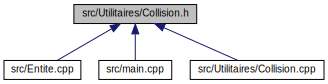
\includegraphics[width=350pt]{_collision_8h__dep__incl}
\end{center}
\end{figure}
\subsection*{Fonctions}
\begin{DoxyCompactItemize}
\item 
bool \hyperlink{_collision_8h_a9037d2ebead3fc780ff50019012ac010}{collision} (const sf\+::\+Shape \&s1, const sf\+::\+Shape \&s2)
\item 
bool \hyperlink{_collision_8h_ad5b149f81d5c820b0f81e5ca66385dee}{collision\+\_\+impl} (const sf\+::\+Shape \&s1, const sf\+::\+Shape \&s2)
\item 
bool \hyperlink{_collision_8h_a4a4d2e91bbfd88f8aaaeb1572140a024}{collision\+\_\+impl} (const sf\+::\+Circle\+Shape \&c1, const sf\+::\+Circle\+Shape \&c2)
\item 
bool \hyperlink{_collision_8h_a598969c4bf7355123d972d3cf69eafd5}{collision\+\_\+impl} (const sf\+::\+Circle\+Shape \&c, const sf\+::\+Shape \&co)
\item 
bool \hyperlink{_collision_8h_adcae147b4b5b0ca770cfbc5b1c65873d}{collision\+\_\+impl} (const sf\+::\+Shape \&co, const sf\+::\+Circle\+Shape \&c)
\end{DoxyCompactItemize}


\subsection{Documentation des fonctions}
\mbox{\Hypertarget{_collision_8h_a9037d2ebead3fc780ff50019012ac010}\label{_collision_8h_a9037d2ebead3fc780ff50019012ac010}} 
\index{Collision.\+h@{Collision.\+h}!collision@{collision}}
\index{collision@{collision}!Collision.\+h@{Collision.\+h}}
\subsubsection{\texorpdfstring{collision()}{collision()}}
{\footnotesize\ttfamily bool collision (\begin{DoxyParamCaption}\item[{const sf\+::\+Shape \&}]{s1,  }\item[{const sf\+::\+Shape \&}]{s2 }\end{DoxyParamCaption})}

\mbox{\Hypertarget{_collision_8h_ad5b149f81d5c820b0f81e5ca66385dee}\label{_collision_8h_ad5b149f81d5c820b0f81e5ca66385dee}} 
\index{Collision.\+h@{Collision.\+h}!collision\+\_\+impl@{collision\+\_\+impl}}
\index{collision\+\_\+impl@{collision\+\_\+impl}!Collision.\+h@{Collision.\+h}}
\subsubsection{\texorpdfstring{collision\+\_\+impl()}{collision\_impl()}\hspace{0.1cm}{\footnotesize\ttfamily [1/4]}}
{\footnotesize\ttfamily bool collision\+\_\+impl (\begin{DoxyParamCaption}\item[{const sf\+::\+Shape \&}]{s1,  }\item[{const sf\+::\+Shape \&}]{s2 }\end{DoxyParamCaption})}

\mbox{\Hypertarget{_collision_8h_a4a4d2e91bbfd88f8aaaeb1572140a024}\label{_collision_8h_a4a4d2e91bbfd88f8aaaeb1572140a024}} 
\index{Collision.\+h@{Collision.\+h}!collision\+\_\+impl@{collision\+\_\+impl}}
\index{collision\+\_\+impl@{collision\+\_\+impl}!Collision.\+h@{Collision.\+h}}
\subsubsection{\texorpdfstring{collision\+\_\+impl()}{collision\_impl()}\hspace{0.1cm}{\footnotesize\ttfamily [2/4]}}
{\footnotesize\ttfamily bool collision\+\_\+impl (\begin{DoxyParamCaption}\item[{const sf\+::\+Circle\+Shape \&}]{c1,  }\item[{const sf\+::\+Circle\+Shape \&}]{c2 }\end{DoxyParamCaption})}

\mbox{\Hypertarget{_collision_8h_a598969c4bf7355123d972d3cf69eafd5}\label{_collision_8h_a598969c4bf7355123d972d3cf69eafd5}} 
\index{Collision.\+h@{Collision.\+h}!collision\+\_\+impl@{collision\+\_\+impl}}
\index{collision\+\_\+impl@{collision\+\_\+impl}!Collision.\+h@{Collision.\+h}}
\subsubsection{\texorpdfstring{collision\+\_\+impl()}{collision\_impl()}\hspace{0.1cm}{\footnotesize\ttfamily [3/4]}}
{\footnotesize\ttfamily bool collision\+\_\+impl (\begin{DoxyParamCaption}\item[{const sf\+::\+Circle\+Shape \&}]{c,  }\item[{const sf\+::\+Shape \&}]{co }\end{DoxyParamCaption})}

\mbox{\Hypertarget{_collision_8h_adcae147b4b5b0ca770cfbc5b1c65873d}\label{_collision_8h_adcae147b4b5b0ca770cfbc5b1c65873d}} 
\index{Collision.\+h@{Collision.\+h}!collision\+\_\+impl@{collision\+\_\+impl}}
\index{collision\+\_\+impl@{collision\+\_\+impl}!Collision.\+h@{Collision.\+h}}
\subsubsection{\texorpdfstring{collision\+\_\+impl()}{collision\_impl()}\hspace{0.1cm}{\footnotesize\ttfamily [4/4]}}
{\footnotesize\ttfamily bool collision\+\_\+impl (\begin{DoxyParamCaption}\item[{const sf\+::\+Shape \&}]{co,  }\item[{const sf\+::\+Circle\+Shape \&}]{c }\end{DoxyParamCaption})}


\hypertarget{_divers_8cpp}{}\section{src/\+Utilitaires/\+Divers.cpp File Reference}
\label{_divers_8cpp}\index{src/\+Utilitaires/\+Divers.\+cpp@{src/\+Utilitaires/\+Divers.\+cpp}}
{\ttfamily \#include \char`\"{}Divers.\+h\char`\"{}}\newline
{\ttfamily \#include \char`\"{}../constantes.\+h\char`\"{}}\newline
{\ttfamily \#include $<$S\+F\+M\+L/\+Graphics.\+hpp$>$}\newline
{\ttfamily \#include $<$algorithm$>$}\newline
{\ttfamily \#include $<$cctype$>$}\newline
\subsection*{Functions}
\begin{DoxyCompactItemize}
\item 
void \mbox{\hyperlink{_divers_8cpp_aeabc946ae0fa583e72aff6e8b7e6cbbc}{adapt\+\_\+viewport}} (sf\+::\+Render\+Window \&window)
\item 
std\+::string \mbox{\hyperlink{_divers_8cpp_a9b855aac79a01bc69b093a4ee12bb688}{trim}} (std\+::string str)
\item 
std\+::pair$<$ std\+::string, std\+::string $>$ \mbox{\hyperlink{_divers_8cpp_a9a29f7315011778d15db9366fbcbe556}{tokenize}} (const std\+::string \&str, char sep)
\item 
double \mbox{\hyperlink{_divers_8cpp_afe48d80943fa9e3ea1f39998f66213a7}{rayon\+\_\+englobeur}} (const std\+::vector$<$ std\+::unique\+\_\+ptr$<$ sf\+::\+Shape $>$$>$ \&forme, sf\+::\+Vector2f origine)
\item 
void \mbox{\hyperlink{_divers_8cpp_afffd86758e1fafd47919e5874a1e93f6}{englobeur\+\_\+circulaire}} (\mbox{\hyperlink{class_entite}{Entite}} \&entite)
\end{DoxyCompactItemize}


\subsection{Function Documentation}
\mbox{\Hypertarget{_divers_8cpp_aeabc946ae0fa583e72aff6e8b7e6cbbc}\label{_divers_8cpp_aeabc946ae0fa583e72aff6e8b7e6cbbc}} 
\index{Divers.\+cpp@{Divers.\+cpp}!adapt\+\_\+viewport@{adapt\+\_\+viewport}}
\index{adapt\+\_\+viewport@{adapt\+\_\+viewport}!Divers.\+cpp@{Divers.\+cpp}}
\subsubsection{\texorpdfstring{adapt\+\_\+viewport()}{adapt\_viewport()}}
{\footnotesize\ttfamily void adapt\+\_\+viewport (\begin{DoxyParamCaption}\item[{sf\+::\+Render\+Window \&}]{window }\end{DoxyParamCaption})}

\mbox{\Hypertarget{_divers_8cpp_afffd86758e1fafd47919e5874a1e93f6}\label{_divers_8cpp_afffd86758e1fafd47919e5874a1e93f6}} 
\index{Divers.\+cpp@{Divers.\+cpp}!englobeur\+\_\+circulaire@{englobeur\+\_\+circulaire}}
\index{englobeur\+\_\+circulaire@{englobeur\+\_\+circulaire}!Divers.\+cpp@{Divers.\+cpp}}
\subsubsection{\texorpdfstring{englobeur\+\_\+circulaire()}{englobeur\_circulaire()}}
{\footnotesize\ttfamily void englobeur\+\_\+circulaire (\begin{DoxyParamCaption}\item[{\mbox{\hyperlink{class_entite}{Entite}} \&}]{entite }\end{DoxyParamCaption})}

\mbox{\Hypertarget{_divers_8cpp_afe48d80943fa9e3ea1f39998f66213a7}\label{_divers_8cpp_afe48d80943fa9e3ea1f39998f66213a7}} 
\index{Divers.\+cpp@{Divers.\+cpp}!rayon\+\_\+englobeur@{rayon\+\_\+englobeur}}
\index{rayon\+\_\+englobeur@{rayon\+\_\+englobeur}!Divers.\+cpp@{Divers.\+cpp}}
\subsubsection{\texorpdfstring{rayon\+\_\+englobeur()}{rayon\_englobeur()}}
{\footnotesize\ttfamily double rayon\+\_\+englobeur (\begin{DoxyParamCaption}\item[{const std\+::vector$<$ std\+::unique\+\_\+ptr$<$ sf\+::\+Shape $>$$>$ \&}]{forme,  }\item[{sf\+::\+Vector2f}]{origine }\end{DoxyParamCaption})}

\mbox{\Hypertarget{_divers_8cpp_a9a29f7315011778d15db9366fbcbe556}\label{_divers_8cpp_a9a29f7315011778d15db9366fbcbe556}} 
\index{Divers.\+cpp@{Divers.\+cpp}!tokenize@{tokenize}}
\index{tokenize@{tokenize}!Divers.\+cpp@{Divers.\+cpp}}
\subsubsection{\texorpdfstring{tokenize()}{tokenize()}}
{\footnotesize\ttfamily std\+::pair$<$std\+::string, std\+::string$>$ tokenize (\begin{DoxyParamCaption}\item[{const std\+::string \&}]{str,  }\item[{char}]{sep }\end{DoxyParamCaption})}

\mbox{\Hypertarget{_divers_8cpp_a9b855aac79a01bc69b093a4ee12bb688}\label{_divers_8cpp_a9b855aac79a01bc69b093a4ee12bb688}} 
\index{Divers.\+cpp@{Divers.\+cpp}!trim@{trim}}
\index{trim@{trim}!Divers.\+cpp@{Divers.\+cpp}}
\subsubsection{\texorpdfstring{trim()}{trim()}}
{\footnotesize\ttfamily std\+::string trim (\begin{DoxyParamCaption}\item[{std\+::string}]{str }\end{DoxyParamCaption})}


\hypertarget{_divers_8h}{}\section{Référence du fichier src/\+Utilitaires/\+Divers.h}
\label{_divers_8h}\index{src/\+Utilitaires/\+Divers.\+h@{src/\+Utilitaires/\+Divers.\+h}}
{\ttfamily \#include $<$type\+\_\+traits$>$}\newline
Graphe des dépendances par inclusion de Divers.\+h\+:\nopagebreak
\begin{figure}[H]
\begin{center}
\leavevmode
\includegraphics[width=194pt]{_divers_8h__incl}
\end{center}
\end{figure}
Ce graphe montre quels fichiers incluent directement ou indirectement ce fichier \+:\nopagebreak
\begin{figure}[H]
\begin{center}
\leavevmode
\includegraphics[width=194pt]{_divers_8h__dep__incl}
\end{center}
\end{figure}
\subsection*{Fonctions}
\begin{DoxyCompactItemize}
\item 
{\footnotesize template$<$typename T , typename U $>$ }\\bool \hyperlink{_divers_8h_a3b8884aabd0ad28b2d790bf0752f6984}{est} (const T \&X)
\end{DoxyCompactItemize}


\subsection{Documentation des fonctions}
\mbox{\Hypertarget{_divers_8h_a3b8884aabd0ad28b2d790bf0752f6984}\label{_divers_8h_a3b8884aabd0ad28b2d790bf0752f6984}} 
\index{Divers.\+h@{Divers.\+h}!est@{est}}
\index{est@{est}!Divers.\+h@{Divers.\+h}}
\subsubsection{\texorpdfstring{est()}{est()}}
{\footnotesize\ttfamily template$<$typename T , typename U $>$ \\
bool est (\begin{DoxyParamCaption}\item[{const T \&}]{X }\end{DoxyParamCaption})}


\hypertarget{optional_8h}{}\section{src/\+Utilitaires/optional.h File Reference}
\label{optional_8h}\index{src/\+Utilitaires/optional.\+h@{src/\+Utilitaires/optional.\+h}}
{\ttfamily \#include $<$utility$>$}\newline
{\ttfamily \#include $<$type\+\_\+traits$>$}\newline
{\ttfamily \#include $<$initializer\+\_\+list$>$}\newline
{\ttfamily \#include $<$cassert$>$}\newline
{\ttfamily \#include $<$functional$>$}\newline
{\ttfamily \#include $<$string$>$}\newline
{\ttfamily \#include $<$stdexcept$>$}\newline
\subsection*{Classes}
\begin{DoxyCompactItemize}
\item 
struct \mbox{\hyperlink{structstd_1_1experimental_1_1is__nothrow__move__constructible}{std\+::experimental\+::is\+\_\+nothrow\+\_\+move\+\_\+constructible$<$ T $>$}}
\item 
struct \mbox{\hyperlink{structstd_1_1experimental_1_1is__assignable}{std\+::experimental\+::is\+\_\+assignable$<$ T, U $>$}}
\item 
struct \mbox{\hyperlink{structstd_1_1experimental_1_1is__nothrow__move__assignable}{std\+::experimental\+::is\+\_\+nothrow\+\_\+move\+\_\+assignable$<$ T $>$}}
\item 
struct \mbox{\hyperlink{structstd_1_1experimental_1_1is__nothrow__move__assignable_1_1has__nothrow__move__assign}{std\+::experimental\+::is\+\_\+nothrow\+\_\+move\+\_\+assignable$<$ T $>$\+::has\+\_\+nothrow\+\_\+move\+\_\+assign$<$ X, has\+\_\+any\+\_\+move\+\_\+assign $>$}}
\item 
struct \mbox{\hyperlink{structstd_1_1experimental_1_1is__nothrow__move__assignable_1_1has__nothrow__move__assign_3_01_x_00_01true_01_4}{std\+::experimental\+::is\+\_\+nothrow\+\_\+move\+\_\+assignable$<$ T $>$\+::has\+\_\+nothrow\+\_\+move\+\_\+assign$<$ X, true $>$}}
\item 
class \mbox{\hyperlink{classstd_1_1experimental_1_1optional}{std\+::experimental\+::optional$<$ T $>$}}
\item 
struct \mbox{\hyperlink{structstd_1_1experimental_1_1detail___1_1has__overloaded__addressof}{std\+::experimental\+::detail\+\_\+\+::has\+\_\+overloaded\+\_\+addressof$<$ T $>$}}
\item 
struct \mbox{\hyperlink{structstd_1_1experimental_1_1trivial__init__t}{std\+::experimental\+::trivial\+\_\+init\+\_\+t}}
\item 
struct \mbox{\hyperlink{structstd_1_1experimental_1_1in__place__t}{std\+::experimental\+::in\+\_\+place\+\_\+t}}
\item 
struct \mbox{\hyperlink{structstd_1_1experimental_1_1nullopt__t}{std\+::experimental\+::nullopt\+\_\+t}}
\item 
struct \mbox{\hyperlink{structstd_1_1experimental_1_1nullopt__t_1_1init}{std\+::experimental\+::nullopt\+\_\+t\+::init}}
\item 
class \mbox{\hyperlink{classstd_1_1experimental_1_1bad__optional__access}{std\+::experimental\+::bad\+\_\+optional\+\_\+access}}
\item 
union \mbox{\hyperlink{unionstd_1_1experimental_1_1storage__t}{std\+::experimental\+::storage\+\_\+t$<$ T $>$}}
\item 
union \mbox{\hyperlink{unionstd_1_1experimental_1_1constexpr__storage__t}{std\+::experimental\+::constexpr\+\_\+storage\+\_\+t$<$ T $>$}}
\item 
struct \mbox{\hyperlink{structstd_1_1experimental_1_1optional__base}{std\+::experimental\+::optional\+\_\+base$<$ T $>$}}
\item 
struct \mbox{\hyperlink{structstd_1_1experimental_1_1constexpr__optional__base}{std\+::experimental\+::constexpr\+\_\+optional\+\_\+base$<$ T $>$}}
\item 
class \mbox{\hyperlink{classstd_1_1experimental_1_1optional}{std\+::experimental\+::optional$<$ T $>$}}
\item 
class \mbox{\hyperlink{classstd_1_1experimental_1_1optional_3_01_t_01_6_01_4}{std\+::experimental\+::optional$<$ T \& $>$}}
\item 
class \mbox{\hyperlink{classstd_1_1experimental_1_1optional_3_01_t_01_6_6_01_4}{std\+::experimental\+::optional$<$ T \&\& $>$}}
\item 
struct \mbox{\hyperlink{structstd_1_1hash_3_01std_1_1experimental_1_1optional_3_01_t_01_4_01_4}{std\+::hash$<$ std\+::experimental\+::optional$<$ T $>$ $>$}}
\item 
struct \mbox{\hyperlink{structstd_1_1hash_3_01std_1_1experimental_1_1optional_3_01_t_01_6_01_4_01_4}{std\+::hash$<$ std\+::experimental\+::optional$<$ T \& $>$ $>$}}
\end{DoxyCompactItemize}
\subsection*{Namespaces}
\begin{DoxyCompactItemize}
\item 
 \mbox{\hyperlink{namespacestd}{std}}
\item 
 \mbox{\hyperlink{namespacestd_1_1experimental}{std\+::experimental}}
\item 
 \mbox{\hyperlink{namespacestd_1_1experimental_1_1detail__}{std\+::experimental\+::detail\+\_\+}}
\end{DoxyCompactItemize}
\subsection*{Macros}
\begin{DoxyCompactItemize}
\item 
\#define \mbox{\hyperlink{optional_8h_a2bc77cf029dcdedaf87668a8da6e899b}{T\+R2\+\_\+\+O\+P\+T\+I\+O\+N\+A\+L\+\_\+\+R\+E\+Q\+U\+I\+R\+ES}}(...)~typename enable\+\_\+if$<$\+\_\+\+\_\+\+V\+A\+\_\+\+A\+R\+G\+S\+\_\+\+\_\+\+::value, bool$>$\+::type = false
\item 
\#define \mbox{\hyperlink{optional_8h_a2fb97d4b996dbddf95c6c25b64e5abb5}{O\+P\+T\+I\+O\+N\+A\+L\+\_\+\+H\+A\+S\+\_\+\+T\+H\+I\+S\+\_\+\+R\+V\+A\+L\+U\+E\+\_\+\+R\+E\+FS}}~0
\item 
\#define \mbox{\hyperlink{optional_8h_af240286c9615958c84d4e886d29022e2}{O\+P\+T\+I\+O\+N\+A\+L\+\_\+\+H\+A\+S\+\_\+\+C\+O\+N\+S\+T\+E\+X\+P\+R\+\_\+\+I\+N\+I\+T\+\_\+\+L\+I\+ST}}~0
\item 
\#define \mbox{\hyperlink{optional_8h_a7399114ed1c146a67741cdd1f681fcb5}{O\+P\+T\+I\+O\+N\+A\+L\+\_\+\+C\+O\+N\+S\+T\+E\+X\+P\+R\+\_\+\+I\+N\+I\+T\+\_\+\+L\+I\+ST}}
\item 
\#define \mbox{\hyperlink{optional_8h_a6e00fbaad952db7aa7f8a701e49ec8f6}{O\+P\+T\+I\+O\+N\+A\+L\+\_\+\+H\+A\+S\+\_\+\+M\+O\+V\+E\+\_\+\+A\+C\+C\+E\+S\+S\+O\+RS}}~0
\item 
\#define \mbox{\hyperlink{optional_8h_af4ab9c6c6aaf518cb24356dbcfa92d90}{O\+P\+T\+I\+O\+N\+A\+L\+\_\+\+M\+U\+T\+A\+B\+L\+E\+\_\+\+C\+O\+N\+S\+T\+E\+X\+PR}}~constexpr
\item 
\#define \mbox{\hyperlink{optional_8h_aba246528349d07cba40ef2d678e6fc78}{T\+R2\+\_\+\+O\+P\+T\+I\+O\+N\+A\+L\+\_\+\+A\+S\+S\+E\+R\+T\+E\+D\+\_\+\+E\+X\+P\+R\+E\+S\+S\+I\+ON}}(C\+H\+E\+CK,  E\+X\+PR)~((C\+H\+E\+CK) ? (E\+X\+PR) \+: (\mbox{[}$\,$\mbox{]}\{assert(!\#C\+H\+E\+CK);\}(), (E\+X\+PR)))
\end{DoxyCompactItemize}
\subsection*{Typedefs}
\begin{DoxyCompactItemize}
\item 
{\footnotesize template$<$typename T $>$ }\\using \mbox{\hyperlink{namespacestd_1_1experimental_a481cc29b2f00961d0afc189e6e90f739}{std\+::experimental\+::is\+\_\+trivially\+\_\+destructible}} = std\+::has\+\_\+trivial\+\_\+destructor$<$ T $>$
\item 
{\footnotesize template$<$class T $>$ }\\using \mbox{\hyperlink{namespacestd_1_1experimental_a33aa5e258a2b0762197365c1ef3f90aa}{std\+::experimental\+::\+Optional\+Base}} = typename std\+::conditional$<$ is\+\_\+trivially\+\_\+destructible$<$ T $>$\+::value, constexpr\+\_\+optional\+\_\+base$<$ typename std\+::remove\+\_\+const$<$ T $>$\+::type $>$, optional\+\_\+base$<$ typename std\+::remove\+\_\+const$<$ T $>$\+::type $>$ $>$\+::type
\end{DoxyCompactItemize}
\subsection*{Functions}
\begin{DoxyCompactItemize}
\item 
{\footnotesize template$<$class T $>$ }\\constexpr T \&\& \mbox{\hyperlink{namespacestd_1_1experimental_ad6c79ef527ee25f0a6295128c4b51f89}{std\+::experimental\+::constexpr\+\_\+forward}} (typename std\+::remove\+\_\+reference$<$ T $>$\+::type \&t) noexcept
\item 
{\footnotesize template$<$class T $>$ }\\constexpr T \&\& \mbox{\hyperlink{namespacestd_1_1experimental_a9bcca6a02f6e3005b3180962429c6feb}{std\+::experimental\+::constexpr\+\_\+forward}} (typename std\+::remove\+\_\+reference$<$ T $>$\+::type \&\&t) noexcept
\item 
{\footnotesize template$<$class T $>$ }\\constexpr std\+::remove\+\_\+reference$<$ T $>$\+::type \&\& \mbox{\hyperlink{namespacestd_1_1experimental_abe16b4d69976581fbfc135b809b3ffe3}{std\+::experimental\+::constexpr\+\_\+move}} (T \&\&t) noexcept
\item 
{\footnotesize template$<$typename T , T\+R2\+\_\+\+O\+P\+T\+I\+O\+N\+A\+L\+\_\+\+R\+E\+Q\+U\+I\+R\+E\+S(!has\+\_\+overloaded\+\_\+addressof$<$ T $>$) $>$ }\\constexpr T $\ast$ \mbox{\hyperlink{namespacestd_1_1experimental_1_1detail___aa205cc382da48555de424fc09d3286b1}{std\+::experimental\+::detail\+\_\+\+::static\+\_\+addressof}} (T \&ref)
\item 
{\footnotesize template$<$typename T , T\+R2\+\_\+\+O\+P\+T\+I\+O\+N\+A\+L\+\_\+\+R\+E\+Q\+U\+I\+R\+E\+S(has\+\_\+overloaded\+\_\+addressof$<$ T $>$) $>$ }\\T $\ast$ \mbox{\hyperlink{namespacestd_1_1experimental_1_1detail___a9255e1a7ac3bf9c92e04e8fb4303f352}{std\+::experimental\+::detail\+\_\+\+::static\+\_\+addressof}} (T \&ref)
\item 
{\footnotesize template$<$class U $>$ }\\constexpr U \mbox{\hyperlink{namespacestd_1_1experimental_1_1detail___a2a47800848ffd486b8ca82d2fbbb244d}{std\+::experimental\+::detail\+\_\+\+::convert}} (U v)
\item 
{\footnotesize template$<$class T $>$ }\\constexpr bool \mbox{\hyperlink{namespacestd_1_1experimental_a0bd6ca198e90eb70255e0b370072f154}{std\+::experimental\+::operator==}} (const optional$<$ T $>$ \&x, const optional$<$ T $>$ \&y)
\item 
{\footnotesize template$<$class T $>$ }\\constexpr bool \mbox{\hyperlink{namespacestd_1_1experimental_abf45cbc40acb4929dbf1caa3b31460d9}{std\+::experimental\+::operator!=}} (const optional$<$ T $>$ \&x, const optional$<$ T $>$ \&y)
\item 
{\footnotesize template$<$class T $>$ }\\constexpr bool \mbox{\hyperlink{namespacestd_1_1experimental_a27caacd2780817469b565c269933185d}{std\+::experimental\+::operator$<$}} (const optional$<$ T $>$ \&x, const optional$<$ T $>$ \&y)
\item 
{\footnotesize template$<$class T $>$ }\\constexpr bool \mbox{\hyperlink{namespacestd_1_1experimental_a1d2409f0cb8fda0ec9a0b9d5e1e61cb5}{std\+::experimental\+::operator$>$}} (const optional$<$ T $>$ \&x, const optional$<$ T $>$ \&y)
\item 
{\footnotesize template$<$class T $>$ }\\constexpr bool \mbox{\hyperlink{namespacestd_1_1experimental_afd5e1ebb8edd29dc3916bf546c9ffca3}{std\+::experimental\+::operator$<$=}} (const optional$<$ T $>$ \&x, const optional$<$ T $>$ \&y)
\item 
{\footnotesize template$<$class T $>$ }\\constexpr bool \mbox{\hyperlink{namespacestd_1_1experimental_a2c2515ef0e94b6089f60aaf6757741c9}{std\+::experimental\+::operator$>$=}} (const optional$<$ T $>$ \&x, const optional$<$ T $>$ \&y)
\item 
{\footnotesize template$<$class T $>$ }\\constexpr bool \mbox{\hyperlink{namespacestd_1_1experimental_a4f15144833bc5951b01fbd4b4bfdb6fb}{std\+::experimental\+::operator==}} (const optional$<$ T $>$ \&x, nullopt\+\_\+t) noexcept
\item 
{\footnotesize template$<$class T $>$ }\\constexpr bool \mbox{\hyperlink{namespacestd_1_1experimental_a23a59ad403fb2809087806ff9037d42e}{std\+::experimental\+::operator==}} (nullopt\+\_\+t, const optional$<$ T $>$ \&x) noexcept
\item 
{\footnotesize template$<$class T $>$ }\\constexpr bool \mbox{\hyperlink{namespacestd_1_1experimental_a768f39fe88fcf07a351e8f45d6dfb1b3}{std\+::experimental\+::operator!=}} (const optional$<$ T $>$ \&x, nullopt\+\_\+t) noexcept
\item 
{\footnotesize template$<$class T $>$ }\\constexpr bool \mbox{\hyperlink{namespacestd_1_1experimental_aa340c9c2a57fd083695e470ded11c089}{std\+::experimental\+::operator!=}} (nullopt\+\_\+t, const optional$<$ T $>$ \&x) noexcept
\item 
{\footnotesize template$<$class T $>$ }\\constexpr bool \mbox{\hyperlink{namespacestd_1_1experimental_aa7075b9ff2db35978c50e744de295b37}{std\+::experimental\+::operator$<$}} (const optional$<$ T $>$ \&, nullopt\+\_\+t) noexcept
\item 
{\footnotesize template$<$class T $>$ }\\constexpr bool \mbox{\hyperlink{namespacestd_1_1experimental_a419ed2da725cc9c030f5d741a1f13d50}{std\+::experimental\+::operator$<$}} (nullopt\+\_\+t, const optional$<$ T $>$ \&x) noexcept
\item 
{\footnotesize template$<$class T $>$ }\\constexpr bool \mbox{\hyperlink{namespacestd_1_1experimental_a2130b2ce528946a4ef4e56f80d823267}{std\+::experimental\+::operator$<$=}} (const optional$<$ T $>$ \&x, nullopt\+\_\+t) noexcept
\item 
{\footnotesize template$<$class T $>$ }\\constexpr bool \mbox{\hyperlink{namespacestd_1_1experimental_ae72fae9caf85b2dff2e94ebd29371937}{std\+::experimental\+::operator$<$=}} (nullopt\+\_\+t, const optional$<$ T $>$ \&) noexcept
\item 
{\footnotesize template$<$class T $>$ }\\constexpr bool \mbox{\hyperlink{namespacestd_1_1experimental_ab0139892916a389ed15c89675d5512ac}{std\+::experimental\+::operator$>$}} (const optional$<$ T $>$ \&x, nullopt\+\_\+t) noexcept
\item 
{\footnotesize template$<$class T $>$ }\\constexpr bool \mbox{\hyperlink{namespacestd_1_1experimental_a02002e302d09fd9596aadd26a38043c0}{std\+::experimental\+::operator$>$}} (nullopt\+\_\+t, const optional$<$ T $>$ \&) noexcept
\item 
{\footnotesize template$<$class T $>$ }\\constexpr bool \mbox{\hyperlink{namespacestd_1_1experimental_a35cdc6a5b56b8db5690f4035242332a0}{std\+::experimental\+::operator$>$=}} (const optional$<$ T $>$ \&, nullopt\+\_\+t) noexcept
\item 
{\footnotesize template$<$class T $>$ }\\constexpr bool \mbox{\hyperlink{namespacestd_1_1experimental_aec1ef0d119fb9270b05212cea79a0fe0}{std\+::experimental\+::operator$>$=}} (nullopt\+\_\+t, const optional$<$ T $>$ \&x) noexcept
\item 
{\footnotesize template$<$class T $>$ }\\constexpr bool \mbox{\hyperlink{namespacestd_1_1experimental_ad40f3ff2c6562139fe910ab3d0a63f10}{std\+::experimental\+::operator==}} (const optional$<$ T $>$ \&x, const T \&v)
\item 
{\footnotesize template$<$class T $>$ }\\constexpr bool \mbox{\hyperlink{namespacestd_1_1experimental_a1958e649d145d612bc04a821d28c0ffb}{std\+::experimental\+::operator==}} (const T \&v, const optional$<$ T $>$ \&x)
\item 
{\footnotesize template$<$class T $>$ }\\constexpr bool \mbox{\hyperlink{namespacestd_1_1experimental_a65194017839ffdd2eeeb2f8f510d9a84}{std\+::experimental\+::operator!=}} (const optional$<$ T $>$ \&x, const T \&v)
\item 
{\footnotesize template$<$class T $>$ }\\constexpr bool \mbox{\hyperlink{namespacestd_1_1experimental_aa6a14a4a2f99c053eaf12e4d438786cc}{std\+::experimental\+::operator!=}} (const T \&v, const optional$<$ T $>$ \&x)
\item 
{\footnotesize template$<$class T $>$ }\\constexpr bool \mbox{\hyperlink{namespacestd_1_1experimental_acd496ce7fb815b5ed07c64c3c50473a5}{std\+::experimental\+::operator$<$}} (const optional$<$ T $>$ \&x, const T \&v)
\item 
{\footnotesize template$<$class T $>$ }\\constexpr bool \mbox{\hyperlink{namespacestd_1_1experimental_a2c15354bc231381036462b92afd3737e}{std\+::experimental\+::operator$>$}} (const T \&v, const optional$<$ T $>$ \&x)
\item 
{\footnotesize template$<$class T $>$ }\\constexpr bool \mbox{\hyperlink{namespacestd_1_1experimental_acd392a8263ad2dd322655078d53e77ad}{std\+::experimental\+::operator$>$}} (const optional$<$ T $>$ \&x, const T \&v)
\item 
{\footnotesize template$<$class T $>$ }\\constexpr bool \mbox{\hyperlink{namespacestd_1_1experimental_a1d3cd046025f9693e0c6c7e57c67e379}{std\+::experimental\+::operator$<$}} (const T \&v, const optional$<$ T $>$ \&x)
\item 
{\footnotesize template$<$class T $>$ }\\constexpr bool \mbox{\hyperlink{namespacestd_1_1experimental_a3209ada3ae8542ffbdfcc7e7d35f19a5}{std\+::experimental\+::operator$>$=}} (const optional$<$ T $>$ \&x, const T \&v)
\item 
{\footnotesize template$<$class T $>$ }\\constexpr bool \mbox{\hyperlink{namespacestd_1_1experimental_a4482ae3dc6aad99b5d17a3a2c0dfe30f}{std\+::experimental\+::operator$<$=}} (const T \&v, const optional$<$ T $>$ \&x)
\item 
{\footnotesize template$<$class T $>$ }\\constexpr bool \mbox{\hyperlink{namespacestd_1_1experimental_a9dd11e02b37f5d3e9c09a29c7ea7024c}{std\+::experimental\+::operator$<$=}} (const optional$<$ T $>$ \&x, const T \&v)
\item 
{\footnotesize template$<$class T $>$ }\\constexpr bool \mbox{\hyperlink{namespacestd_1_1experimental_a0e2303b05ab975b9dd1a53c198bf2e45}{std\+::experimental\+::operator$>$=}} (const T \&v, const optional$<$ T $>$ \&x)
\item 
{\footnotesize template$<$class T $>$ }\\constexpr bool \mbox{\hyperlink{namespacestd_1_1experimental_a5e8049d714e136368d3f1cc2cc7fc787}{std\+::experimental\+::operator==}} (const optional$<$ T \&$>$ \&x, const T \&v)
\item 
{\footnotesize template$<$class T $>$ }\\constexpr bool \mbox{\hyperlink{namespacestd_1_1experimental_ad874f9e082998b503ad0f7bb0376782e}{std\+::experimental\+::operator==}} (const T \&v, const optional$<$ T \&$>$ \&x)
\item 
{\footnotesize template$<$class T $>$ }\\constexpr bool \mbox{\hyperlink{namespacestd_1_1experimental_a32e202bafe91eccccc3d34ef53bc3f01}{std\+::experimental\+::operator!=}} (const optional$<$ T \&$>$ \&x, const T \&v)
\item 
{\footnotesize template$<$class T $>$ }\\constexpr bool \mbox{\hyperlink{namespacestd_1_1experimental_aa2bc218261382e5d1dbb90aee5930580}{std\+::experimental\+::operator!=}} (const T \&v, const optional$<$ T \&$>$ \&x)
\item 
{\footnotesize template$<$class T $>$ }\\constexpr bool \mbox{\hyperlink{namespacestd_1_1experimental_a83a84dd901351c69fb0e53efe17526eb}{std\+::experimental\+::operator$<$}} (const optional$<$ T \&$>$ \&x, const T \&v)
\item 
{\footnotesize template$<$class T $>$ }\\constexpr bool \mbox{\hyperlink{namespacestd_1_1experimental_a84d294fc6ef231696e23f6b21f0391aa}{std\+::experimental\+::operator$>$}} (const T \&v, const optional$<$ T \&$>$ \&x)
\item 
{\footnotesize template$<$class T $>$ }\\constexpr bool \mbox{\hyperlink{namespacestd_1_1experimental_a733d2aa90d49bd113f2420f996e13a8f}{std\+::experimental\+::operator$>$}} (const optional$<$ T \&$>$ \&x, const T \&v)
\item 
{\footnotesize template$<$class T $>$ }\\constexpr bool \mbox{\hyperlink{namespacestd_1_1experimental_ae8fc20bba7e30d2ad7bc8646ec1de715}{std\+::experimental\+::operator$<$}} (const T \&v, const optional$<$ T \&$>$ \&x)
\item 
{\footnotesize template$<$class T $>$ }\\constexpr bool \mbox{\hyperlink{namespacestd_1_1experimental_a8e331f49161fae9a2dc83a0838d5c332}{std\+::experimental\+::operator$>$=}} (const optional$<$ T \&$>$ \&x, const T \&v)
\item 
{\footnotesize template$<$class T $>$ }\\constexpr bool \mbox{\hyperlink{namespacestd_1_1experimental_a59ad44110fa8b750e2ca4cf69327c182}{std\+::experimental\+::operator$<$=}} (const T \&v, const optional$<$ T \&$>$ \&x)
\item 
{\footnotesize template$<$class T $>$ }\\constexpr bool \mbox{\hyperlink{namespacestd_1_1experimental_adeee1539a6ebda9088aaaa92a363a38c}{std\+::experimental\+::operator$<$=}} (const optional$<$ T \&$>$ \&x, const T \&v)
\item 
{\footnotesize template$<$class T $>$ }\\constexpr bool \mbox{\hyperlink{namespacestd_1_1experimental_af08a779caea9116149f04d2b2e330b44}{std\+::experimental\+::operator$>$=}} (const T \&v, const optional$<$ T \&$>$ \&x)
\item 
{\footnotesize template$<$class T $>$ }\\constexpr bool \mbox{\hyperlink{namespacestd_1_1experimental_ad41e06efa15d85ead93eafecb8dde126}{std\+::experimental\+::operator==}} (const optional$<$ const T \&$>$ \&x, const T \&v)
\item 
{\footnotesize template$<$class T $>$ }\\constexpr bool \mbox{\hyperlink{namespacestd_1_1experimental_a9ff726fa7b981eeae6f6b8e98eb514ce}{std\+::experimental\+::operator==}} (const T \&v, const optional$<$ const T \&$>$ \&x)
\item 
{\footnotesize template$<$class T $>$ }\\constexpr bool \mbox{\hyperlink{namespacestd_1_1experimental_a007e24ca3b589918778709281a5611d7}{std\+::experimental\+::operator!=}} (const optional$<$ const T \&$>$ \&x, const T \&v)
\item 
{\footnotesize template$<$class T $>$ }\\constexpr bool \mbox{\hyperlink{namespacestd_1_1experimental_ab5a8b15ec09913c93bac27399f0cba38}{std\+::experimental\+::operator!=}} (const T \&v, const optional$<$ const T \&$>$ \&x)
\item 
{\footnotesize template$<$class T $>$ }\\constexpr bool \mbox{\hyperlink{namespacestd_1_1experimental_afd3f43608dc3267d32ee592ae88fba55}{std\+::experimental\+::operator$<$}} (const optional$<$ const T \&$>$ \&x, const T \&v)
\item 
{\footnotesize template$<$class T $>$ }\\constexpr bool \mbox{\hyperlink{namespacestd_1_1experimental_a3899be1cf909f9d5dc2718c912c73d67}{std\+::experimental\+::operator$>$}} (const T \&v, const optional$<$ const T \&$>$ \&x)
\item 
{\footnotesize template$<$class T $>$ }\\constexpr bool \mbox{\hyperlink{namespacestd_1_1experimental_ab62a91459215563e8996e69785166789}{std\+::experimental\+::operator$>$}} (const optional$<$ const T \&$>$ \&x, const T \&v)
\item 
{\footnotesize template$<$class T $>$ }\\constexpr bool \mbox{\hyperlink{namespacestd_1_1experimental_a3905d16fb3b1c1627ff2082e6159d4fb}{std\+::experimental\+::operator$<$}} (const T \&v, const optional$<$ const T \&$>$ \&x)
\item 
{\footnotesize template$<$class T $>$ }\\constexpr bool \mbox{\hyperlink{namespacestd_1_1experimental_a43c159cf8ffd0e172adbac601809aacd}{std\+::experimental\+::operator$>$=}} (const optional$<$ const T \&$>$ \&x, const T \&v)
\item 
{\footnotesize template$<$class T $>$ }\\constexpr bool \mbox{\hyperlink{namespacestd_1_1experimental_aca22cd45974dad371a24b9618f2d1b33}{std\+::experimental\+::operator$<$=}} (const T \&v, const optional$<$ const T \&$>$ \&x)
\item 
{\footnotesize template$<$class T $>$ }\\constexpr bool \mbox{\hyperlink{namespacestd_1_1experimental_afb3a1b869e0a3eb4840f37edf61ba0ef}{std\+::experimental\+::operator$<$=}} (const optional$<$ const T \&$>$ \&x, const T \&v)
\item 
{\footnotesize template$<$class T $>$ }\\constexpr bool \mbox{\hyperlink{namespacestd_1_1experimental_a943314dada174c65a0ac853cbdc89989}{std\+::experimental\+::operator$>$=}} (const T \&v, const optional$<$ const T \&$>$ \&x)
\item 
{\footnotesize template$<$class T $>$ }\\void \mbox{\hyperlink{namespacestd_1_1experimental_acdfba2d2e9c79f689a34c9cea5c5682d}{std\+::experimental\+::swap}} (optional$<$ T $>$ \&x, optional$<$ T $>$ \&y) noexcept(noexcept(x.\+swap(y)))
\item 
{\footnotesize template$<$class T $>$ }\\constexpr optional$<$ typename decay$<$ T $>$\+::type $>$ \mbox{\hyperlink{namespacestd_1_1experimental_aa6c8db3625ec5a8e7f6288fb5adf8f95}{std\+::experimental\+::make\+\_\+optional}} (T \&\&v)
\item 
{\footnotesize template$<$class X $>$ }\\constexpr optional$<$ X \& $>$ \mbox{\hyperlink{namespacestd_1_1experimental_a0f7b286ddf3bb6c4e95580898dcde37b}{std\+::experimental\+::make\+\_\+optional}} (reference\+\_\+wrapper$<$ X $>$ v)
\end{DoxyCompactItemize}
\subsection*{Variables}
\begin{DoxyCompactItemize}
\item 
constexpr struct \mbox{\hyperlink{structstd_1_1experimental_1_1trivial__init__t}{std\+::experimental\+::trivial\+\_\+init\+\_\+t}} \mbox{\hyperlink{namespacestd_1_1experimental_a453a56e465f134032297679f0511f02b}{std\+::experimental\+::trivial\+\_\+init}}
\item 
constexpr struct \mbox{\hyperlink{structstd_1_1experimental_1_1in__place__t}{std\+::experimental\+::in\+\_\+place\+\_\+t}} \mbox{\hyperlink{namespacestd_1_1experimental_a93be82cb49ba2dc64a23c881ad152fd6}{std\+::experimental\+::in\+\_\+place}}
\item 
constexpr nullopt\+\_\+t \mbox{\hyperlink{namespacestd_1_1experimental_af16e944368340cafdc29647c42a1f542}{std\+::experimental\+::nullopt}} \{nullopt\+\_\+t\+::init()\}
\end{DoxyCompactItemize}


\subsection{Macro Definition Documentation}
\mbox{\Hypertarget{optional_8h_a7399114ed1c146a67741cdd1f681fcb5}\label{optional_8h_a7399114ed1c146a67741cdd1f681fcb5}} 
\index{optional.\+h@{optional.\+h}!O\+P\+T\+I\+O\+N\+A\+L\+\_\+\+C\+O\+N\+S\+T\+E\+X\+P\+R\+\_\+\+I\+N\+I\+T\+\_\+\+L\+I\+ST@{O\+P\+T\+I\+O\+N\+A\+L\+\_\+\+C\+O\+N\+S\+T\+E\+X\+P\+R\+\_\+\+I\+N\+I\+T\+\_\+\+L\+I\+ST}}
\index{O\+P\+T\+I\+O\+N\+A\+L\+\_\+\+C\+O\+N\+S\+T\+E\+X\+P\+R\+\_\+\+I\+N\+I\+T\+\_\+\+L\+I\+ST@{O\+P\+T\+I\+O\+N\+A\+L\+\_\+\+C\+O\+N\+S\+T\+E\+X\+P\+R\+\_\+\+I\+N\+I\+T\+\_\+\+L\+I\+ST}!optional.\+h@{optional.\+h}}
\subsubsection{\texorpdfstring{O\+P\+T\+I\+O\+N\+A\+L\+\_\+\+C\+O\+N\+S\+T\+E\+X\+P\+R\+\_\+\+I\+N\+I\+T\+\_\+\+L\+I\+ST}{OPTIONAL\_CONSTEXPR\_INIT\_LIST}}
{\footnotesize\ttfamily \#define O\+P\+T\+I\+O\+N\+A\+L\+\_\+\+C\+O\+N\+S\+T\+E\+X\+P\+R\+\_\+\+I\+N\+I\+T\+\_\+\+L\+I\+ST}

\mbox{\Hypertarget{optional_8h_af240286c9615958c84d4e886d29022e2}\label{optional_8h_af240286c9615958c84d4e886d29022e2}} 
\index{optional.\+h@{optional.\+h}!O\+P\+T\+I\+O\+N\+A\+L\+\_\+\+H\+A\+S\+\_\+\+C\+O\+N\+S\+T\+E\+X\+P\+R\+\_\+\+I\+N\+I\+T\+\_\+\+L\+I\+ST@{O\+P\+T\+I\+O\+N\+A\+L\+\_\+\+H\+A\+S\+\_\+\+C\+O\+N\+S\+T\+E\+X\+P\+R\+\_\+\+I\+N\+I\+T\+\_\+\+L\+I\+ST}}
\index{O\+P\+T\+I\+O\+N\+A\+L\+\_\+\+H\+A\+S\+\_\+\+C\+O\+N\+S\+T\+E\+X\+P\+R\+\_\+\+I\+N\+I\+T\+\_\+\+L\+I\+ST@{O\+P\+T\+I\+O\+N\+A\+L\+\_\+\+H\+A\+S\+\_\+\+C\+O\+N\+S\+T\+E\+X\+P\+R\+\_\+\+I\+N\+I\+T\+\_\+\+L\+I\+ST}!optional.\+h@{optional.\+h}}
\subsubsection{\texorpdfstring{O\+P\+T\+I\+O\+N\+A\+L\+\_\+\+H\+A\+S\+\_\+\+C\+O\+N\+S\+T\+E\+X\+P\+R\+\_\+\+I\+N\+I\+T\+\_\+\+L\+I\+ST}{OPTIONAL\_HAS\_CONSTEXPR\_INIT\_LIST}}
{\footnotesize\ttfamily \#define O\+P\+T\+I\+O\+N\+A\+L\+\_\+\+H\+A\+S\+\_\+\+C\+O\+N\+S\+T\+E\+X\+P\+R\+\_\+\+I\+N\+I\+T\+\_\+\+L\+I\+ST~0}

\mbox{\Hypertarget{optional_8h_a6e00fbaad952db7aa7f8a701e49ec8f6}\label{optional_8h_a6e00fbaad952db7aa7f8a701e49ec8f6}} 
\index{optional.\+h@{optional.\+h}!O\+P\+T\+I\+O\+N\+A\+L\+\_\+\+H\+A\+S\+\_\+\+M\+O\+V\+E\+\_\+\+A\+C\+C\+E\+S\+S\+O\+RS@{O\+P\+T\+I\+O\+N\+A\+L\+\_\+\+H\+A\+S\+\_\+\+M\+O\+V\+E\+\_\+\+A\+C\+C\+E\+S\+S\+O\+RS}}
\index{O\+P\+T\+I\+O\+N\+A\+L\+\_\+\+H\+A\+S\+\_\+\+M\+O\+V\+E\+\_\+\+A\+C\+C\+E\+S\+S\+O\+RS@{O\+P\+T\+I\+O\+N\+A\+L\+\_\+\+H\+A\+S\+\_\+\+M\+O\+V\+E\+\_\+\+A\+C\+C\+E\+S\+S\+O\+RS}!optional.\+h@{optional.\+h}}
\subsubsection{\texorpdfstring{O\+P\+T\+I\+O\+N\+A\+L\+\_\+\+H\+A\+S\+\_\+\+M\+O\+V\+E\+\_\+\+A\+C\+C\+E\+S\+S\+O\+RS}{OPTIONAL\_HAS\_MOVE\_ACCESSORS}}
{\footnotesize\ttfamily \#define O\+P\+T\+I\+O\+N\+A\+L\+\_\+\+H\+A\+S\+\_\+\+M\+O\+V\+E\+\_\+\+A\+C\+C\+E\+S\+S\+O\+RS~0}

\mbox{\Hypertarget{optional_8h_a2fb97d4b996dbddf95c6c25b64e5abb5}\label{optional_8h_a2fb97d4b996dbddf95c6c25b64e5abb5}} 
\index{optional.\+h@{optional.\+h}!O\+P\+T\+I\+O\+N\+A\+L\+\_\+\+H\+A\+S\+\_\+\+T\+H\+I\+S\+\_\+\+R\+V\+A\+L\+U\+E\+\_\+\+R\+E\+FS@{O\+P\+T\+I\+O\+N\+A\+L\+\_\+\+H\+A\+S\+\_\+\+T\+H\+I\+S\+\_\+\+R\+V\+A\+L\+U\+E\+\_\+\+R\+E\+FS}}
\index{O\+P\+T\+I\+O\+N\+A\+L\+\_\+\+H\+A\+S\+\_\+\+T\+H\+I\+S\+\_\+\+R\+V\+A\+L\+U\+E\+\_\+\+R\+E\+FS@{O\+P\+T\+I\+O\+N\+A\+L\+\_\+\+H\+A\+S\+\_\+\+T\+H\+I\+S\+\_\+\+R\+V\+A\+L\+U\+E\+\_\+\+R\+E\+FS}!optional.\+h@{optional.\+h}}
\subsubsection{\texorpdfstring{O\+P\+T\+I\+O\+N\+A\+L\+\_\+\+H\+A\+S\+\_\+\+T\+H\+I\+S\+\_\+\+R\+V\+A\+L\+U\+E\+\_\+\+R\+E\+FS}{OPTIONAL\_HAS\_THIS\_RVALUE\_REFS}}
{\footnotesize\ttfamily \#define O\+P\+T\+I\+O\+N\+A\+L\+\_\+\+H\+A\+S\+\_\+\+T\+H\+I\+S\+\_\+\+R\+V\+A\+L\+U\+E\+\_\+\+R\+E\+FS~0}

\mbox{\Hypertarget{optional_8h_af4ab9c6c6aaf518cb24356dbcfa92d90}\label{optional_8h_af4ab9c6c6aaf518cb24356dbcfa92d90}} 
\index{optional.\+h@{optional.\+h}!O\+P\+T\+I\+O\+N\+A\+L\+\_\+\+M\+U\+T\+A\+B\+L\+E\+\_\+\+C\+O\+N\+S\+T\+E\+X\+PR@{O\+P\+T\+I\+O\+N\+A\+L\+\_\+\+M\+U\+T\+A\+B\+L\+E\+\_\+\+C\+O\+N\+S\+T\+E\+X\+PR}}
\index{O\+P\+T\+I\+O\+N\+A\+L\+\_\+\+M\+U\+T\+A\+B\+L\+E\+\_\+\+C\+O\+N\+S\+T\+E\+X\+PR@{O\+P\+T\+I\+O\+N\+A\+L\+\_\+\+M\+U\+T\+A\+B\+L\+E\+\_\+\+C\+O\+N\+S\+T\+E\+X\+PR}!optional.\+h@{optional.\+h}}
\subsubsection{\texorpdfstring{O\+P\+T\+I\+O\+N\+A\+L\+\_\+\+M\+U\+T\+A\+B\+L\+E\+\_\+\+C\+O\+N\+S\+T\+E\+X\+PR}{OPTIONAL\_MUTABLE\_CONSTEXPR}}
{\footnotesize\ttfamily \#define O\+P\+T\+I\+O\+N\+A\+L\+\_\+\+M\+U\+T\+A\+B\+L\+E\+\_\+\+C\+O\+N\+S\+T\+E\+X\+PR~constexpr}

\mbox{\Hypertarget{optional_8h_aba246528349d07cba40ef2d678e6fc78}\label{optional_8h_aba246528349d07cba40ef2d678e6fc78}} 
\index{optional.\+h@{optional.\+h}!T\+R2\+\_\+\+O\+P\+T\+I\+O\+N\+A\+L\+\_\+\+A\+S\+S\+E\+R\+T\+E\+D\+\_\+\+E\+X\+P\+R\+E\+S\+S\+I\+ON@{T\+R2\+\_\+\+O\+P\+T\+I\+O\+N\+A\+L\+\_\+\+A\+S\+S\+E\+R\+T\+E\+D\+\_\+\+E\+X\+P\+R\+E\+S\+S\+I\+ON}}
\index{T\+R2\+\_\+\+O\+P\+T\+I\+O\+N\+A\+L\+\_\+\+A\+S\+S\+E\+R\+T\+E\+D\+\_\+\+E\+X\+P\+R\+E\+S\+S\+I\+ON@{T\+R2\+\_\+\+O\+P\+T\+I\+O\+N\+A\+L\+\_\+\+A\+S\+S\+E\+R\+T\+E\+D\+\_\+\+E\+X\+P\+R\+E\+S\+S\+I\+ON}!optional.\+h@{optional.\+h}}
\subsubsection{\texorpdfstring{T\+R2\+\_\+\+O\+P\+T\+I\+O\+N\+A\+L\+\_\+\+A\+S\+S\+E\+R\+T\+E\+D\+\_\+\+E\+X\+P\+R\+E\+S\+S\+I\+ON}{TR2\_OPTIONAL\_ASSERTED\_EXPRESSION}}
{\footnotesize\ttfamily \#define T\+R2\+\_\+\+O\+P\+T\+I\+O\+N\+A\+L\+\_\+\+A\+S\+S\+E\+R\+T\+E\+D\+\_\+\+E\+X\+P\+R\+E\+S\+S\+I\+ON(\begin{DoxyParamCaption}\item[{}]{C\+H\+E\+CK,  }\item[{}]{E\+X\+PR }\end{DoxyParamCaption})~((C\+H\+E\+CK) ? (E\+X\+PR) \+: (\mbox{[}$\,$\mbox{]}\{assert(!\#C\+H\+E\+CK);\}(), (E\+X\+PR)))}

\mbox{\Hypertarget{optional_8h_a2bc77cf029dcdedaf87668a8da6e899b}\label{optional_8h_a2bc77cf029dcdedaf87668a8da6e899b}} 
\index{optional.\+h@{optional.\+h}!T\+R2\+\_\+\+O\+P\+T\+I\+O\+N\+A\+L\+\_\+\+R\+E\+Q\+U\+I\+R\+ES@{T\+R2\+\_\+\+O\+P\+T\+I\+O\+N\+A\+L\+\_\+\+R\+E\+Q\+U\+I\+R\+ES}}
\index{T\+R2\+\_\+\+O\+P\+T\+I\+O\+N\+A\+L\+\_\+\+R\+E\+Q\+U\+I\+R\+ES@{T\+R2\+\_\+\+O\+P\+T\+I\+O\+N\+A\+L\+\_\+\+R\+E\+Q\+U\+I\+R\+ES}!optional.\+h@{optional.\+h}}
\subsubsection{\texorpdfstring{T\+R2\+\_\+\+O\+P\+T\+I\+O\+N\+A\+L\+\_\+\+R\+E\+Q\+U\+I\+R\+ES}{TR2\_OPTIONAL\_REQUIRES}}
{\footnotesize\ttfamily \#define T\+R2\+\_\+\+O\+P\+T\+I\+O\+N\+A\+L\+\_\+\+R\+E\+Q\+U\+I\+R\+ES(\begin{DoxyParamCaption}\item[{}]{... }\end{DoxyParamCaption})~typename enable\+\_\+if$<$\+\_\+\+\_\+\+V\+A\+\_\+\+A\+R\+G\+S\+\_\+\+\_\+\+::value, bool$>$\+::type = false}


\hypertarget{_sounds_8h}{}\section{src/\+Utilitaires/\+Sounds.h File Reference}
\label{_sounds_8h}\index{src/\+Utilitaires/\+Sounds.\+h@{src/\+Utilitaires/\+Sounds.\+h}}

\hypertarget{_trajectoire_8cpp}{}\section{Référence du fichier src/\+Utilitaires/\+Trajectoire.cpp}
\label{_trajectoire_8cpp}\index{src/\+Utilitaires/\+Trajectoire.\+cpp@{src/\+Utilitaires/\+Trajectoire.\+cpp}}
{\ttfamily \#include \char`\"{}Trajectoire.\+h\char`\"{}}\newline
{\ttfamily \#include \char`\"{}../constantes.\+h\char`\"{}}\newline
Graphe des dépendances par inclusion de Trajectoire.\+cpp\+:\nopagebreak
\begin{figure}[H]
\begin{center}
\leavevmode
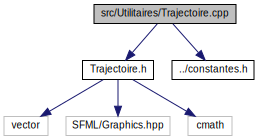
\includegraphics[width=330pt]{_trajectoire_8cpp__incl}
\end{center}
\end{figure}
\subsection*{Fonctions}
\begin{DoxyCompactItemize}
\item 
sf\+::\+Vector2f \hyperlink{_trajectoire_8cpp_acb6b19dacbcb60977ea16b36c5888404}{traj\+\_\+position} (\hyperlink{_trajectoire_8h_afa7f6e8323d7ee755d93cd1f6019dd95}{Trajectoire} trajectoire, float t, float vit\+\_\+, sf\+::\+Vector2f pos\+Init, std\+::vector$<$ float $>$ params)
\end{DoxyCompactItemize}


\subsection{Documentation des fonctions}
\mbox{\Hypertarget{_trajectoire_8cpp_acb6b19dacbcb60977ea16b36c5888404}\label{_trajectoire_8cpp_acb6b19dacbcb60977ea16b36c5888404}} 
\index{Trajectoire.\+cpp@{Trajectoire.\+cpp}!traj\+\_\+position@{traj\+\_\+position}}
\index{traj\+\_\+position@{traj\+\_\+position}!Trajectoire.\+cpp@{Trajectoire.\+cpp}}
\subsubsection{\texorpdfstring{traj\+\_\+position()}{traj\_position()}}
{\footnotesize\ttfamily sf\+::\+Vector2f traj\+\_\+position (\begin{DoxyParamCaption}\item[{\hyperlink{_trajectoire_8h_afa7f6e8323d7ee755d93cd1f6019dd95}{Trajectoire}}]{trajectoire,  }\item[{float}]{t,  }\item[{float}]{vit\+\_\+,  }\item[{sf\+::\+Vector2f}]{pos\+Init,  }\item[{std\+::vector$<$ float $>$}]{params }\end{DoxyParamCaption})}


\hypertarget{_trajectoire_8h}{}\section{Référence du fichier src/\+Utilitaires/\+Trajectoire.h}
\label{_trajectoire_8h}\index{src/\+Utilitaires/\+Trajectoire.\+h@{src/\+Utilitaires/\+Trajectoire.\+h}}
{\ttfamily \#include $<$vector$>$}\newline
{\ttfamily \#include $<$S\+F\+M\+L/\+Graphics.\+hpp$>$}\newline
{\ttfamily \#include $<$cmath$>$}\newline
Graphe des dépendances par inclusion de Trajectoire.\+h\+:\nopagebreak
\begin{figure}[H]
\begin{center}
\leavevmode
\includegraphics[width=308pt]{_trajectoire_8h__incl}
\end{center}
\end{figure}
Ce graphe montre quels fichiers incluent directement ou indirectement ce fichier \+:
% FIG 0
\subsection*{Énumérations}
\begin{DoxyCompactItemize}
\item 
enum \hyperlink{_trajectoire_8h_afa7f6e8323d7ee755d93cd1f6019dd95}{Trajectoire} \{ \hyperlink{_trajectoire_8h_afa7f6e8323d7ee755d93cd1f6019dd95a8bc010f4818a3f1553fbb13140ef7764}{L\+I\+N\+E\+A\+I\+RE}, 
\hyperlink{_trajectoire_8h_afa7f6e8323d7ee755d93cd1f6019dd95a2e1c07250c4de3cf6c0db9a42dd0870b}{P\+A\+R\+A\+B\+O\+L\+I\+Q\+UE}, 
\hyperlink{_trajectoire_8h_afa7f6e8323d7ee755d93cd1f6019dd95a33f374dc94a3ff34a023886c4e6e7102}{S\+I\+N\+US}, 
\hyperlink{_trajectoire_8h_afa7f6e8323d7ee755d93cd1f6019dd95a90e1b7efef28fa0dc94c0af827f8c5a9}{M\+O\+U\+T\+ON}
 \}\begin{DoxyCompactList}\small\item\em liste énumérée des types possibles de trajectoire \end{DoxyCompactList}
\end{DoxyCompactItemize}
\subsection*{Fonctions}
\begin{DoxyCompactItemize}
\item 
sf\+::\+Vector2f \hyperlink{_trajectoire_8h_acb6b19dacbcb60977ea16b36c5888404}{traj\+\_\+position} (\hyperlink{_trajectoire_8h_afa7f6e8323d7ee755d93cd1f6019dd95}{Trajectoire} trajectoire, float t, float vit\+\_\+, sf\+::\+Vector2f pos\+Init, std\+::vector$<$ float $>$ params)
\end{DoxyCompactItemize}


\subsection{Documentation du type de l\textquotesingle{}énumération}
\mbox{\Hypertarget{_trajectoire_8h_afa7f6e8323d7ee755d93cd1f6019dd95}\label{_trajectoire_8h_afa7f6e8323d7ee755d93cd1f6019dd95}} 
\index{Trajectoire.\+h@{Trajectoire.\+h}!Trajectoire@{Trajectoire}}
\index{Trajectoire@{Trajectoire}!Trajectoire.\+h@{Trajectoire.\+h}}
\subsubsection{\texorpdfstring{Trajectoire}{Trajectoire}}
{\footnotesize\ttfamily enum \hyperlink{_trajectoire_8h_afa7f6e8323d7ee755d93cd1f6019dd95}{Trajectoire}}



liste énumérée des types possibles de trajectoire 

\begin{DoxyEnumFields}{Valeurs énumérées}
\raisebox{\heightof{T}}[0pt][0pt]{\index{L\+I\+N\+E\+A\+I\+RE@{L\+I\+N\+E\+A\+I\+RE}!Trajectoire.\+h@{Trajectoire.\+h}}\index{Trajectoire.\+h@{Trajectoire.\+h}!L\+I\+N\+E\+A\+I\+RE@{L\+I\+N\+E\+A\+I\+RE}}}\mbox{\Hypertarget{_trajectoire_8h_afa7f6e8323d7ee755d93cd1f6019dd95a8bc010f4818a3f1553fbb13140ef7764}\label{_trajectoire_8h_afa7f6e8323d7ee755d93cd1f6019dd95a8bc010f4818a3f1553fbb13140ef7764}} 
L\+I\+N\+E\+A\+I\+RE&\\
\hline

\raisebox{\heightof{T}}[0pt][0pt]{\index{P\+A\+R\+A\+B\+O\+L\+I\+Q\+UE@{P\+A\+R\+A\+B\+O\+L\+I\+Q\+UE}!Trajectoire.\+h@{Trajectoire.\+h}}\index{Trajectoire.\+h@{Trajectoire.\+h}!P\+A\+R\+A\+B\+O\+L\+I\+Q\+UE@{P\+A\+R\+A\+B\+O\+L\+I\+Q\+UE}}}\mbox{\Hypertarget{_trajectoire_8h_afa7f6e8323d7ee755d93cd1f6019dd95a2e1c07250c4de3cf6c0db9a42dd0870b}\label{_trajectoire_8h_afa7f6e8323d7ee755d93cd1f6019dd95a2e1c07250c4de3cf6c0db9a42dd0870b}} 
P\+A\+R\+A\+B\+O\+L\+I\+Q\+UE&\\
\hline

\raisebox{\heightof{T}}[0pt][0pt]{\index{S\+I\+N\+US@{S\+I\+N\+US}!Trajectoire.\+h@{Trajectoire.\+h}}\index{Trajectoire.\+h@{Trajectoire.\+h}!S\+I\+N\+US@{S\+I\+N\+US}}}\mbox{\Hypertarget{_trajectoire_8h_afa7f6e8323d7ee755d93cd1f6019dd95a33f374dc94a3ff34a023886c4e6e7102}\label{_trajectoire_8h_afa7f6e8323d7ee755d93cd1f6019dd95a33f374dc94a3ff34a023886c4e6e7102}} 
S\+I\+N\+US&\\
\hline

\raisebox{\heightof{T}}[0pt][0pt]{\index{M\+O\+U\+T\+ON@{M\+O\+U\+T\+ON}!Trajectoire.\+h@{Trajectoire.\+h}}\index{Trajectoire.\+h@{Trajectoire.\+h}!M\+O\+U\+T\+ON@{M\+O\+U\+T\+ON}}}\mbox{\Hypertarget{_trajectoire_8h_afa7f6e8323d7ee755d93cd1f6019dd95a90e1b7efef28fa0dc94c0af827f8c5a9}\label{_trajectoire_8h_afa7f6e8323d7ee755d93cd1f6019dd95a90e1b7efef28fa0dc94c0af827f8c5a9}} 
M\+O\+U\+T\+ON&\\
\hline

\end{DoxyEnumFields}


\subsection{Documentation des fonctions}
\mbox{\Hypertarget{_trajectoire_8h_acb6b19dacbcb60977ea16b36c5888404}\label{_trajectoire_8h_acb6b19dacbcb60977ea16b36c5888404}} 
\index{Trajectoire.\+h@{Trajectoire.\+h}!traj\+\_\+position@{traj\+\_\+position}}
\index{traj\+\_\+position@{traj\+\_\+position}!Trajectoire.\+h@{Trajectoire.\+h}}
\subsubsection{\texorpdfstring{traj\+\_\+position()}{traj\_position()}}
{\footnotesize\ttfamily sf\+::\+Vector2f traj\+\_\+position (\begin{DoxyParamCaption}\item[{\hyperlink{_trajectoire_8h_afa7f6e8323d7ee755d93cd1f6019dd95}{Trajectoire}}]{trajectoire,  }\item[{float}]{t,  }\item[{float}]{vit\+\_\+,  }\item[{sf\+::\+Vector2f}]{pos\+Init,  }\item[{std\+::vector$<$ float $>$}]{params }\end{DoxyParamCaption})}


\hypertarget{__vaisseaux_8h}{}\section{Référence du fichier src/\+Vaisseau/\+\_\+vaisseaux.h}
\label{__vaisseaux_8h}\index{src/\+Vaisseau/\+\_\+vaisseaux.\+h@{src/\+Vaisseau/\+\_\+vaisseaux.\+h}}
{\ttfamily \#include \char`\"{}Vaisseau\+Eclaireur.\+h\char`\"{}}\newline
{\ttfamily \#include \char`\"{}Vaisseau\+Test.\+h\char`\"{}}\newline
Graphe des dépendances par inclusion de \+\_\+vaisseaux.\+h\+:\nopagebreak
\begin{figure}[H]
\begin{center}
\leavevmode
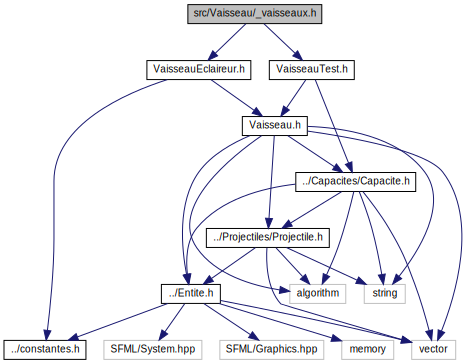
\includegraphics[width=350pt]{__vaisseaux_8h__incl}
\end{center}
\end{figure}
Ce graphe montre quels fichiers incluent directement ou indirectement ce fichier \+:\nopagebreak
\begin{figure}[H]
\begin{center}
\leavevmode
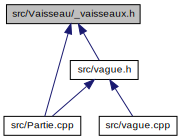
\includegraphics[width=214pt]{__vaisseaux_8h__dep__incl}
\end{center}
\end{figure}

\hypertarget{_vaiss_bouclier_8cpp}{}\section{src/\+Vaisseau/\+Vaiss\+Bouclier.cpp File Reference}
\label{_vaiss_bouclier_8cpp}\index{src/\+Vaisseau/\+Vaiss\+Bouclier.\+cpp@{src/\+Vaisseau/\+Vaiss\+Bouclier.\+cpp}}
{\ttfamily \#include \char`\"{}Vaiss\+Bouclier.\+h\char`\"{}}\newline
{\ttfamily \#include $<$cmath$>$}\newline

\hypertarget{_vaiss_bouclier_8h}{}\section{src/\+Vaisseau/\+Vaiss\+Bouclier.h File Reference}
\label{_vaiss_bouclier_8h}\index{src/\+Vaisseau/\+Vaiss\+Bouclier.\+h@{src/\+Vaisseau/\+Vaiss\+Bouclier.\+h}}
{\ttfamily \#include \char`\"{}Vaisseau.\+h\char`\"{}}\newline
\subsection*{Classes}
\begin{DoxyCompactItemize}
\item 
class \mbox{\hyperlink{class_vaiss_bouclier}{Vaiss\+Bouclier}}
\begin{DoxyCompactList}\small\item\em classe du bouclier du \mbox{\hyperlink{class_vaisseau_defenseur}{Vaisseau\+Defenseur}} \end{DoxyCompactList}\end{DoxyCompactItemize}

\hypertarget{_vaisseau_8cpp}{}\section{Référence du fichier src/\+Vaisseau.cpp}
\label{_vaisseau_8cpp}\index{src/\+Vaisseau.\+cpp@{src/\+Vaisseau.\+cpp}}
{\ttfamily \#include $<$vector$>$}\newline
{\ttfamily \#include $<$string$>$}\newline
{\ttfamily \#include $<$algorithm$>$}\newline
{\ttfamily \#include \char`\"{}Capacite.\+h\char`\"{}}\newline
{\ttfamily \#include \char`\"{}Vaisseau.\+h\char`\"{}}\newline
{\ttfamily \#include \char`\"{}Projectile.\+h\char`\"{}}\newline
Graphe des dépendances par inclusion de Vaisseau.\+cpp\+:\nopagebreak
\begin{figure}[H]
\begin{center}
\leavevmode
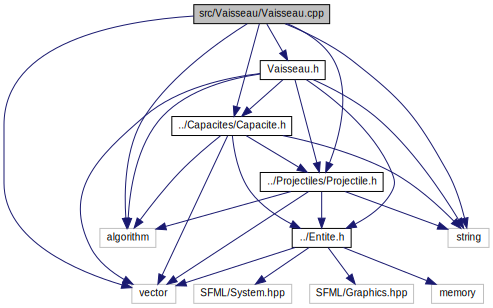
\includegraphics[width=328pt]{_vaisseau_8cpp__incl}
\end{center}
\end{figure}

\hypertarget{_vaisseau_8h}{}\section{Référence du fichier src/\+Vaisseau/\+Vaisseau.h}
\label{_vaisseau_8h}\index{src/\+Vaisseau/\+Vaisseau.\+h@{src/\+Vaisseau/\+Vaisseau.\+h}}
{\ttfamily \#include $<$vector$>$}\newline
{\ttfamily \#include $<$string$>$}\newline
{\ttfamily \#include $<$algorithm$>$}\newline
{\ttfamily \#include \char`\"{}../\+Capacites/\+Capacite.\+h\char`\"{}}\newline
{\ttfamily \#include \char`\"{}../\+Entite.\+h\char`\"{}}\newline
{\ttfamily \#include \char`\"{}../\+Projectiles/\+Projectile.\+h\char`\"{}}\newline
{\ttfamily \#include \char`\"{}../\+Interface/\+Input.\+h\char`\"{}}\newline
Graphe des dépendances par inclusion de Vaisseau.\+h\+:\nopagebreak
\begin{figure}[H]
\begin{center}
\leavevmode
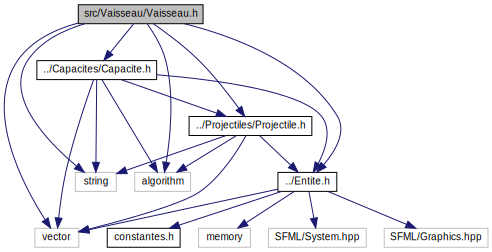
\includegraphics[width=350pt]{_vaisseau_8h__incl}
\end{center}
\end{figure}
Ce graphe montre quels fichiers incluent directement ou indirectement ce fichier \+:\nopagebreak
\begin{figure}[H]
\begin{center}
\leavevmode
\includegraphics[width=350pt]{_vaisseau_8h__dep__incl}
\end{center}
\end{figure}
\subsection*{Classes}
\begin{DoxyCompactItemize}
\item 
class \hyperlink{class_vaisseau}{Vaisseau}
\begin{DoxyCompactList}\small\item\em classe du vaisseau (véhicule) d\textquotesingle{}un joueur ou d\textquotesingle{}un ennemi \end{DoxyCompactList}\end{DoxyCompactItemize}

\hypertarget{_vaisseau_attaquant_8cpp}{}\section{Référence du fichier src/\+Vaisseau/\+Vaisseau\+Attaquant.cpp}
\label{_vaisseau_attaquant_8cpp}\index{src/\+Vaisseau/\+Vaisseau\+Attaquant.\+cpp@{src/\+Vaisseau/\+Vaisseau\+Attaquant.\+cpp}}
{\ttfamily \#include \char`\"{}Vaisseau\+Attaquant.\+h\char`\"{}}\newline
{\ttfamily \#include $<$cmath$>$}\newline
Graphe des dépendances par inclusion de Vaisseau\+Attaquant.\+cpp\+:\nopagebreak
\begin{figure}[H]
\begin{center}
\leavevmode
\includegraphics[width=350pt]{_vaisseau_attaquant_8cpp__incl}
\end{center}
\end{figure}

\hypertarget{_vaisseau_attaquant_8h}{}\section{src/\+Vaisseau/\+Vaisseau\+Attaquant.h File Reference}
\label{_vaisseau_attaquant_8h}\index{src/\+Vaisseau/\+Vaisseau\+Attaquant.\+h@{src/\+Vaisseau/\+Vaisseau\+Attaquant.\+h}}
{\ttfamily \#include \char`\"{}../constantes.\+h\char`\"{}}\newline
{\ttfamily \#include \char`\"{}Vaisseau.\+h\char`\"{}}\newline
{\ttfamily \#include \char`\"{}../\+Capacites/\+Cap\+Missile.\+h\char`\"{}}\newline
{\ttfamily \#include \char`\"{}../\+Utilitaires/\+Trajectoire.\+h\char`\"{}}\newline
\subsection*{Classes}
\begin{DoxyCompactItemize}
\item 
class \mbox{\hyperlink{class_vaisseau_attaquant}{Vaisseau\+Attaquant}}
\begin{DoxyCompactList}\small\item\em classe d\textquotesingle{}un ennemi de base \+: l\textquotesingle{}attaquant \end{DoxyCompactList}\end{DoxyCompactItemize}

\hypertarget{_vaisseau_defenseur_8cpp}{}\section{Référence du fichier src/\+Vaisseau/\+Vaisseau\+Defenseur.cpp}
\label{_vaisseau_defenseur_8cpp}\index{src/\+Vaisseau/\+Vaisseau\+Defenseur.\+cpp@{src/\+Vaisseau/\+Vaisseau\+Defenseur.\+cpp}}
{\ttfamily \#include \char`\"{}Vaisseau\+Defenseur.\+h\char`\"{}}\newline
{\ttfamily \#include $<$cmath$>$}\newline
Graphe des dépendances par inclusion de Vaisseau\+Defenseur.\+cpp\+:
% FIG 0

\hypertarget{_vaisseau_defenseur_8h}{}\section{src/\+Vaisseau/\+Vaisseau\+Defenseur.h File Reference}
\label{_vaisseau_defenseur_8h}\index{src/\+Vaisseau/\+Vaisseau\+Defenseur.\+h@{src/\+Vaisseau/\+Vaisseau\+Defenseur.\+h}}
{\ttfamily \#include $<$vector$>$}\newline
{\ttfamily \#include \char`\"{}../constantes.\+h\char`\"{}}\newline
{\ttfamily \#include \char`\"{}Vaisseau.\+h\char`\"{}}\newline
{\ttfamily \#include \char`\"{}../\+Utilitaires/\+Trajectoire.\+h\char`\"{}}\newline
{\ttfamily \#include \char`\"{}Vaiss\+Bouclier.\+h\char`\"{}}\newline
\subsection*{Classes}
\begin{DoxyCompactItemize}
\item 
class \mbox{\hyperlink{class_vaisseau_defenseur}{Vaisseau\+Defenseur}}
\end{DoxyCompactItemize}

\hypertarget{_vaisseau_eclaireur_8cpp}{}\section{Référence du fichier src/\+Vaisseau/\+Vaisseau\+Eclaireur.cpp}
\label{_vaisseau_eclaireur_8cpp}\index{src/\+Vaisseau/\+Vaisseau\+Eclaireur.\+cpp@{src/\+Vaisseau/\+Vaisseau\+Eclaireur.\+cpp}}
{\ttfamily \#include \char`\"{}Vaisseau\+Eclaireur.\+h\char`\"{}}\newline
{\ttfamily \#include $<$cmath$>$}\newline
Graphe des dépendances par inclusion de Vaisseau\+Eclaireur.\+cpp\+:
% FIG 0

\hypertarget{_vaisseau_eclaireur_8h}{}\section{src/\+Vaisseau/\+Vaisseau\+Eclaireur.h File Reference}
\label{_vaisseau_eclaireur_8h}\index{src/\+Vaisseau/\+Vaisseau\+Eclaireur.\+h@{src/\+Vaisseau/\+Vaisseau\+Eclaireur.\+h}}
{\ttfamily \#include $<$vector$>$}\newline
{\ttfamily \#include \char`\"{}../constantes.\+h\char`\"{}}\newline
{\ttfamily \#include \char`\"{}Vaisseau.\+h\char`\"{}}\newline
{\ttfamily \#include \char`\"{}../\+Utilitaires/\+Trajectoire.\+h\char`\"{}}\newline
\subsection*{Classes}
\begin{DoxyCompactItemize}
\item 
class \mbox{\hyperlink{class_vaisseau_eclaireur}{Vaisseau\+Eclaireur}}
\begin{DoxyCompactList}\small\item\em classe d\textquotesingle{}un ennemi de base \+: l\textquotesingle{}éclaireur \end{DoxyCompactList}\end{DoxyCompactItemize}

\hypertarget{_vaisseau_test_8cpp}{}\section{src/\+Vaisseau/\+Vaisseau\+Test.cpp File Reference}
\label{_vaisseau_test_8cpp}\index{src/\+Vaisseau/\+Vaisseau\+Test.\+cpp@{src/\+Vaisseau/\+Vaisseau\+Test.\+cpp}}
{\ttfamily \#include \char`\"{}Vaisseau\+Test.\+h\char`\"{}}\newline
{\ttfamily \#include $<$cmath$>$}\newline

\hypertarget{_vaisseau_test_8h}{}\section{Référence du fichier src/\+Vaisseau/\+Vaisseau\+Test.h}
\label{_vaisseau_test_8h}\index{src/\+Vaisseau/\+Vaisseau\+Test.\+h@{src/\+Vaisseau/\+Vaisseau\+Test.\+h}}
{\ttfamily \#include \char`\"{}Vaisseau.\+h\char`\"{}}\newline
{\ttfamily \#include \char`\"{}../\+Capacites/\+Capacite.\+h\char`\"{}}\newline
Graphe des dépendances par inclusion de Vaisseau\+Test.\+h\+:
\nopagebreak
\begin{figure}[H]
\begin{center}
\leavevmode
\includegraphics[width=350pt]{_vaisseau_test_8h__incl}
\end{center}
\end{figure}
Ce graphe montre quels fichiers incluent directement ou indirectement ce fichier \+:
\nopagebreak
\begin{figure}[H]
\begin{center}
\leavevmode
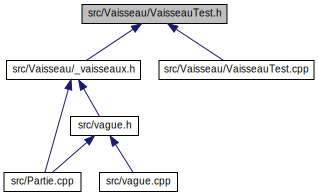
\includegraphics[width=330pt]{_vaisseau_test_8h__dep__incl}
\end{center}
\end{figure}
\subsection*{Classes}
\begin{DoxyCompactItemize}
\item 
class \hyperlink{class_vaisseau_test}{Vaisseau\+Test}
\end{DoxyCompactItemize}

%--- End generated contents ---

% Index
\backmatter
\newpage
\phantomsection
\clearemptydoublepage
\addcontentsline{toc}{chapter}{Index}
\printindex

\end{document}
